\documentclass[12pt]{article}
\usepackage[utf8]{inputenc}

%%%% Layout %%%%
\usepackage{geometry}
\geometry{a4paper, left=1in, right=1in, top=2in}
\usepackage{hyperref}
\hypersetup{linktoc=all}
\usepackage[toc, page]{appendix}
\usepackage[labelfont=bf, hypcap, labelsep=period, skip=0.5\baselineskip]{caption}
\usepackage{url}
\Urlmuskip=0mu plus 1mu
\usepackage{chngcntr} % Number equations/figures/tables as (section.#)
\counterwithin{equation}{section}
\counterwithin{figure}{section}
\counterwithin{table}{section}

% Make acknowledgements environment similar to the abstract
\newenvironment{acknowledgements}{\renewcommand\abstractname{Acknowledgements}\begin{abstract}} {\end{abstract}}

% Blank page without page number
\usepackage{afterpage}
\newcommand\blankpage{
	\null
	\thispagestyle{empty}
	\addtocounter{page}{-1}
	\newpage}

%%%% Text %%%%
\usepackage{enumerate}
\usepackage{enumitem}

%%%% Math %%%%
\usepackage{mathtools}
\usepackage{amsmath}
\usepackage{amsfonts}
\usepackage{cases}
\DeclareMathSymbol{\shortminus}{\mathbin}{AMSa}{"39}
\usepackage{bbm}
\newcommand{\R}{\mathbbm{R}}

% To number a specific line in an align environment instead of all or no lines
\newcommand\numberthis{\addtocounter{equation}{1}\tag{\theequation}}

% For row reduction operations
\newenvironment{sysmatrix}[1]
{\left(\begin{array}{@{}#1@{}}}
{\end{array}\right)}
\newcommand{\ro}[1]{\xrightarrow{\mathmakebox[\rowidth]{#1}}}
\newlength{\rowidth}% row operation width
\AtBeginDocument{\setlength{\rowidth}{6em}}

%%%% Tables %%%%
\usepackage{dcolumn}
\usepackage{multirow}
\usepackage{booktabs}
\usepackage{xltabular}
\usepackage{float}
\usepackage{lscape}

\usepackage{etoolbox}
\AtBeginEnvironment{longtable}{\footnotesize}{}{}
\AtBeginEnvironment{xltabular}{\footnotesize}{}{}
\AtBeginEnvironment{tabular}{\footnotesize}{}{}

% The following fixes a bug where xltabular breaks booktabs
\makeatletter
\def\@BTrule[#1]{%
	\ifx\longtable\undefined
	\let\@BTswitch\@BTnormal
	\else\ifx\hline\LT@hline
	\nobreak
	\let\@BTswitch\@BLTrule
	\else
	\let\@BTswitch\@BTnormal
	\fi\fi
	\global\@thisrulewidth=#1\relax
	\ifnum\@thisruleclass=\tw@\vskip\@aboverulesep\else
	\ifnum\@lastruleclass=\z@\vskip\@aboverulesep\else
	\ifnum\@lastruleclass=\@ne\vskip\doublerulesep\fi\fi\fi
	\@BTswitch}
\makeatother

%%%% Graphics %%%%
\usepackage{graphicx}
\usepackage{subcaption} % For subfigures
\usepackage[dvipsnames]{xcolor}
% \usepackage{tikz}
% \usetikzlibrary{external}
% \tikzexternalize[prefix=tikz/]
\usepackage{pgfplots}
\pgfplotsset{compat = newest}
\usepackage{rotating}

%%%% TODO notes %%%%
\usepackage{todonotes}
\makeatletter
%  \renewcommand{\todo}[2][]{\tikzexternaldisable\@todo[#1]{#2}\tikzexternalenable}
\makeatother

%%%% Bibliography %%%%
\usepackage[style=apa, backend=biber]{biblatex}
\DeclareLanguageMapping{english}{english-apa}
\addbibresource{thesis.bib}

%%%% Miscellaneous %%%%
% NA

%%%% Begin document %%%%
\title{Master Thesis}
\begin{document}

	\pagenumbering{roman}
	
	\afterpage{\blankpage}
	
	\begin{titlepage}
		\centering
		
		\vfill
		
		
\includegraphics[width=\textwidth]{output/TiuLogo.eps}
		\vskip1.5cm
		{\huge
			Predicting The Incidence Rate And Case Fatality Rate Of COVID-19 in Italy\\
			\large\bigskip
			by\\
			Mike Weltevrede (ANR 756479)\\
			\vskip1.5cm
			A thesis submitted in partial fulfillment of the requirements for the degree of Master in Econometrics and Mathematical Economics.
			\vskip0.5cm
			Tilburg School of Economics and Management\\
			Tilburg University\\
			\vskip1.5cm
			Supervised by:\\
			dr. Otilia Boldea \\
			\vskip0.5cm
			Second reader:\\
			dr. George Knox
			\vfill
			Date:\\
			\today
		}   
		\vfill
		\vfill
	\end{titlepage}
	
	\newpage
	
	\newpage
	
	\begin{abstract}
		TODO
	\end{abstract}
	
	\newpage
	
	% Acknowledgement
	% Your thank-you's fall into three categories: scientific/technical, financial and personal. Scientific and technical persons to consider thanking - your supervisor/s as well as other persons who helped you in the interpretation of your results, or in carrying out the practical aspects of your work, data collection, etc. In terms of finances, you can acknowledge that the research was supported by company X or through Dr. Y. In the last category you might any one that you feel helped you in your studies, in addition to friends or family who lent you support.
	\begin{acknowledgements}
		TODO
	\end{acknowledgements}
	
	\newpage
	
	\tableofcontents
	
	\newpage
	\pagenumbering{arabic}
	
	%Introduction
	\section{Introduction} \label{sec:introduction}
	% Contains literature review, your contribution briefly and how it is new relative to other studies, 1-3 main contributions of your thesis; each contribution should be backed up with one table to be found directly in the text.
	Since the beginning of 2020, severe acute respiratory syndrome coronavirus 2 (SARS-CoV-2) has plagued the world. Starting from Wuhan, China, it has made its way to every single continent apart from Antarctica and (nearly) every country in the world. Only 12 sovereign member states of the United Nations reported no infections, of which 10 are island countries. The other two countries are North Korea and Turkmenistan but it is suspected that there are actually cases but that these are not reported for both North Korea \parencite{businessinsider2020dprk, nebehay2020dprk} and Turkmenistan \parencite{hrw2020turkmenistan, mackinnon2020turkmenistan}. In response to SARS-CoV-2, governments have been implementing far-reaching measures to try and contain the virus, such as shutting down schools and restaurants, but also by locking down the entire country. \\
	
	On August 19, 2020, over 21 million people were reported to have been infected with the infectious respiratory disease caused by SARS-CoV-2, called coronavirus disease 2019 (commonly abbreviated to COVID-19), leading to 771 thousand consequent deaths, while almost 14 million people have already recovered from COVID-19. Therefore, almost 36 million people worldwide have been infected by the virus. On top of this, due to the inherent problem of a limited testing capacity, there are most likely many infections that went and still are going undocumented, meaning that the scope of the problem is much larger than the numbers just mentioned. The World Health Organization (WHO) declared a Public Health Emergency of International Concern (PHEIC) on 30 January 2020 \parencite{who2020pheic}, defined as \textit{``an extraordinary event which is determined to constitute a public health risk to other States through the international spread of disease and to potentially require a coordinated international response”} \parencite{who2019ihr}. After the spread of SARS-CoV-2 only became worse, the WHO declared the virus outbreak to be a pandemic on 11 March 2020 \parencite{who2020pandemic}, where a pandemic is defined as \textit{``an epidemic occurring on worldwide or over a very wide area, crossing international boundaries, and usually affecting a large number of people"} \parencite{porta2014dictionary}. \\
	
	\newpage
	\section{Problem description} \label{sec:problem_description}
	% Description of problem
	In this section, we elaborate on the problem at hand, namely the epidemiological spread of SARS-CoV-2 and the disease it causes, specifically for the country of Italy. We focus on the additions of this thesis to the existing literature. \\
	
	Italy has been one of the most intensely struck countries by COVID-19. Until the end of March, it had the highest number of confirmed cases per 100,000 inhabitants. It was subsequently taken over by Spain. Italy remained the second most struck country until May 1, when the United States took over. On July 3, 2020, it had the ninth highest absolute number of confirmed cases, after the United States, Brazil, Russia, India, Peru, Chile, the United Kingdom, and Spain. Italy reported the second highest global death-to-cases ratio of 14.45\% (34,818 deaths to 240,961 cases), only after the United Kingdom, which reports a death-to-cases ratio of 15.50\% (43,995 deaths to 283,757 cases). The third highest death-to-cases ratio of 12.24\% (29,189 deaths to 238,511 cases) was reported by Mexico. The sudden onset of the spread of SARS-CoV-2 put immense pressure on the Italian hospitals, especially in the northern regions such as Lombardy. This forced patients with coronavirus-caused pneumonia to be sent home as well as literal collapses of overworked healthcare workers \parencite{horowitz2020healthcare}. \\
	
	Due to the extreme nature of the pandemic in Italy and the availability of enough data, this thesis chooses to focus on Italy. Our contribution is to model the pandemic at the regional level rather than at the national level. Even though the regions within Italy are likely more similar to one another than, for instance, to the provinces in the Netherlands, there are large regional differences in Italy as well. This implies that there is not one model that can be used to analyze the entire country of Italy because this would ignore the regional heterogenous effects. Besides doing so to uncover heterogeneity across regions, the regonal variation allows for better identificaton of the average transmission parameters. To illustrate these regional differences, we will present several figures. Firstly, consider Figure \ref{fig:incidence_per_NUTS1}, which shows the incidence rates categorized by the overarching region that the regions are a part of (called NUTS 1 regions). This regional structure is explained more thoroughly in Section \ref{subsec:italy_geography}. \\
	
	\begin{figure}[ht]
	    \centering
	    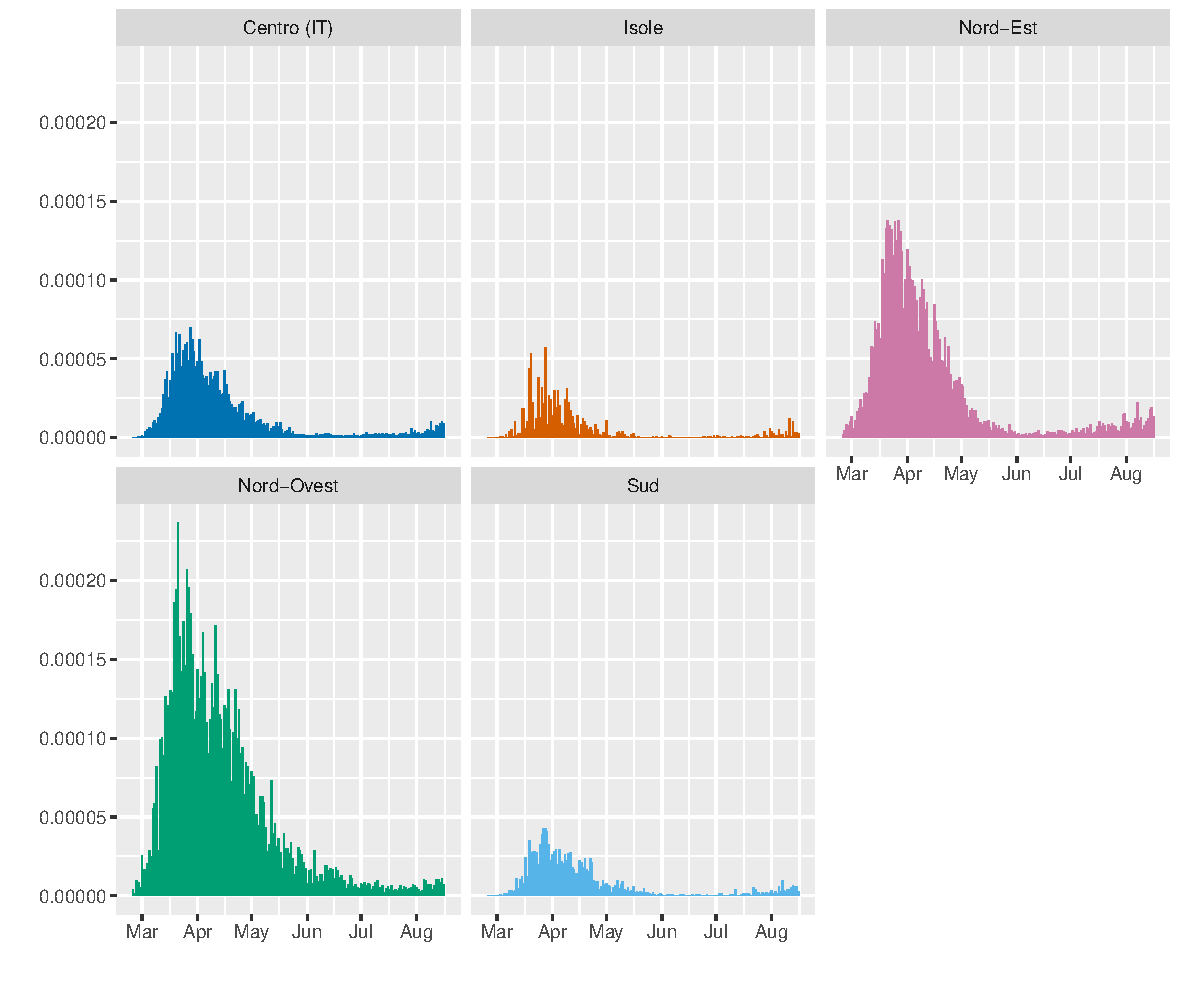
\includegraphics[width=\textwidth]{output/infective_rate_per_NUTS1.pdf}
	    \caption{Incidence rate per NUTS 1 region}
	    \label{fig:incidence_per_NUTS1}
	\end{figure}
	
	In Figure \ref{fig:incidence_per_NUTS1}, we can see that there is a wide difference in the incidence rates between these larger regions. Not only do we see that the heights of the peaks differ, we also notice that the length of the peaks differ slightly over the regions. This already shows that models that pool these regions together, to form the entire country of Italy, are likely less suitable than models that take these differences into account. Similarly, one can imagine that there are even larger differences between the lower level regions. \\ \\ \\
	
	Consider Figure \ref{fig:incidence_Centro}, where we zoom in on the Centro (IT) NUTS 1 region by looking at the four regions that make it up. These lower level regions are called the NUTS 2 regions. The plots for the other NUTS 1 regions can be found in Appendix \ref{sapp:figures_problem_description}. Figure \ref{fig:incidence_Centro} shows us that, even among the regions in the NUTS 1 region, there is a vast difference. For the region of Lazio, we see a much lower peak than for the other three regions, especially compared to Marche. Moreover, the varying length of the peak is more visible in Figure \ref{fig:incidence_Centro}. For instance, compare the regions of Marche and Umbria. \\
	
	\begin{figure}[H]
	    \centering
	    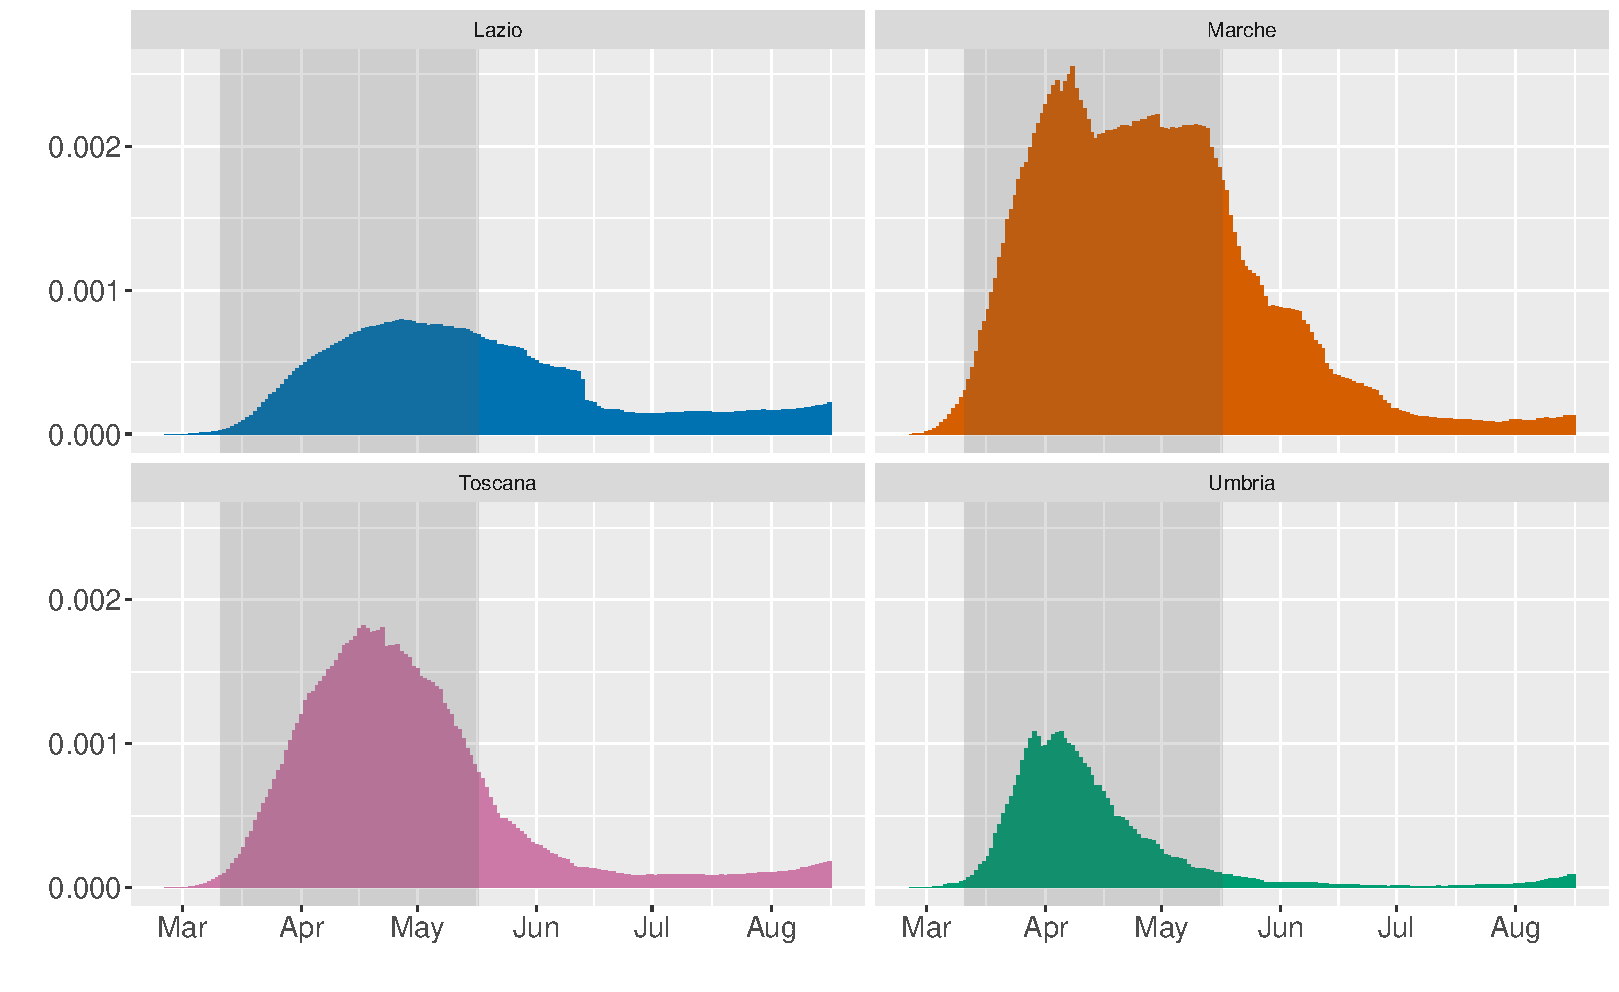
\includegraphics[width=\textwidth]{output/infective_rates_Centro (IT).pdf}
	    \caption{Incidence rate per region for the \textit{Centro (IT)} (Centre) NUTS 1 region}
	    \label{fig:incidence_Centro}
	\end{figure}
	
	We can also investigate the regional heterogeneity by looking at the mean incidence rate over the regions. We consider the mean incidence rate because this allows us to compare regions, even when these have a higher population county. Consider Figure \ref{fig:heterogeneity_over_regions}, which shows the mean incidence rate for the NUTS 2 regions, divided up into their respective NUTS 1 regions. \\
	
	\begin{figure}[ht]
	    \centering
	    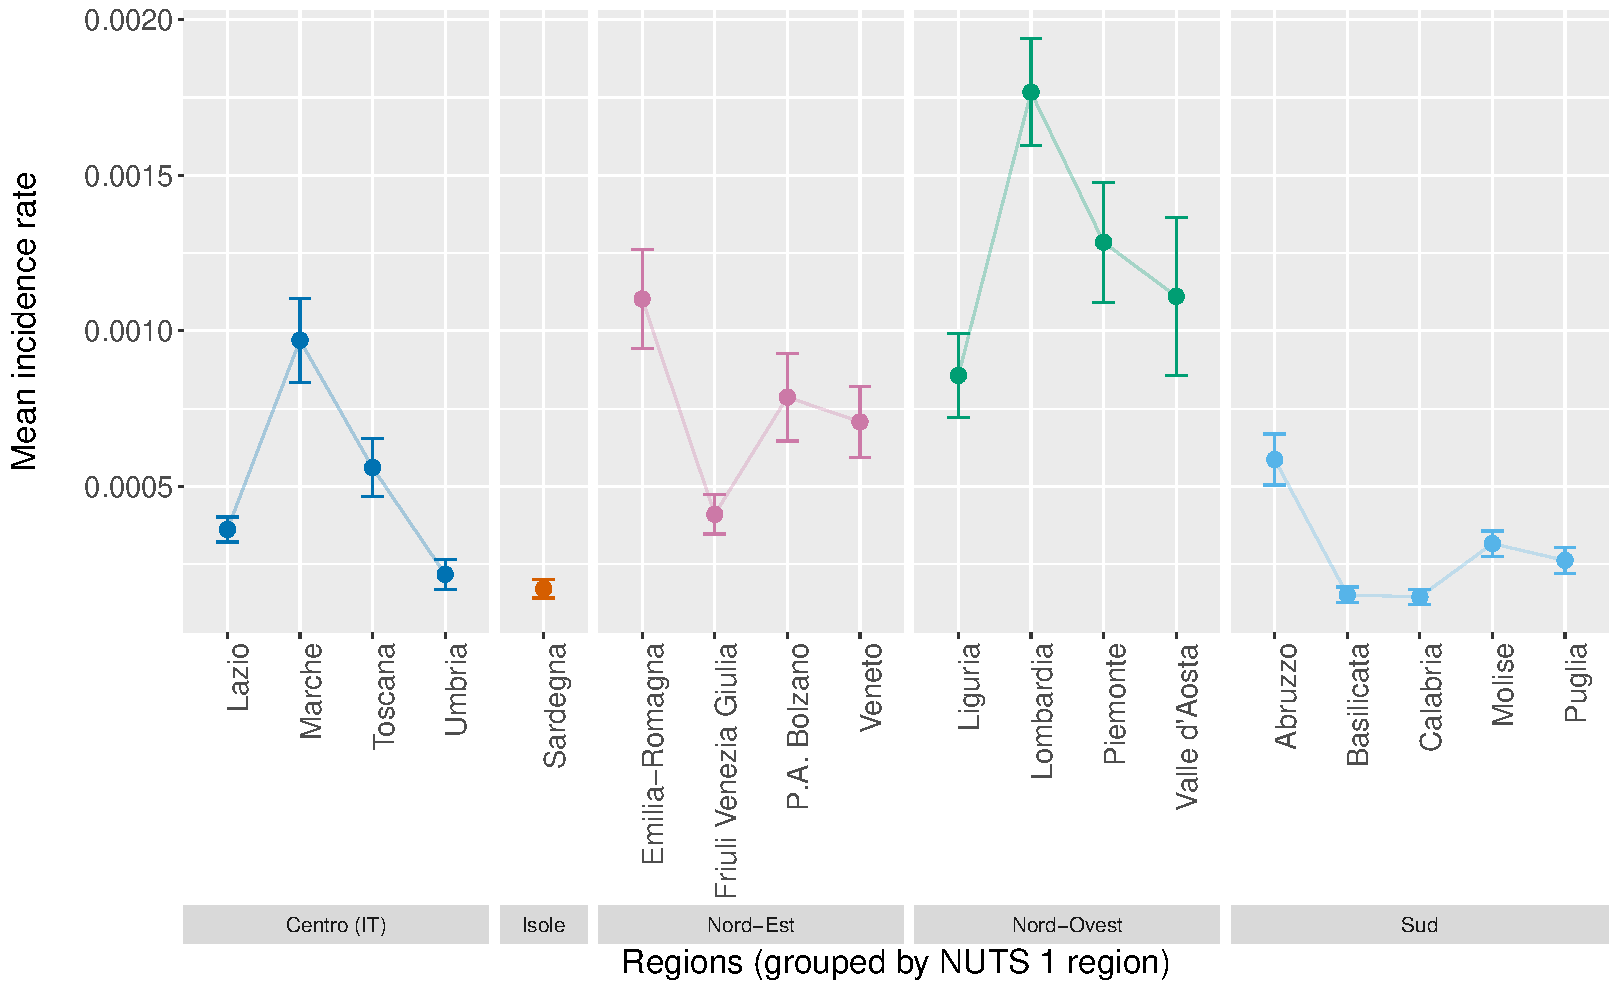
\includegraphics[width=\textwidth]{output/heterogeneity_over_regions.pdf}
	    \caption{Heterogeneity across Italian regions}
	    \label{fig:heterogeneity_over_regions}
	\end{figure}
	
	From Figure \ref{fig:heterogeneity_over_regions}, we can see that there is a large difference in the mean incidence rate over the different regions. Although we see that the mean incidence rates within the same NUTS 1 region are more similar than outside these regions, there is still a proper difference among regions, even in the same NUTS 1 region. To illustrate, consider the \textit{Nord-Est} (North-East) NUTS 1 region. The mean of P.A. Bolzano (Autonomous Province of Bolzano) cannot be statistically distinguished with that of Emilia-Romagna and Veneto, which can be concluded because the given error bars of two times the standard deviation overlap. However, it can be distinguished from the mean incidence rate of Friuli Venezia Giulia, because these error bars do not overlap. This shows us that the heterogeneity between regions can likely not be ignored. \\
	
	In this thesis, we present several models. We are basing the models on specifications as used by \textcite{adda2016economic}. In the paper, \textcite{adda2016economic} investigates the spread of several viral diseases in the past, namely for influenza, gastroenteritis, and chickenpox. The models used to research this spread are inspired by the Standard Inflammatory Response (SIR) model but deviate from the SIR model in the sense that the right-hand side variables include the number of new cases rather than the absolute number of cases. The key additions made by \textcite{adda2016economic} are, firstly, that a spatial spillover effect is considered and, secondly, that some sort of weighting on the parameters is allowed on the basis of region specific variables. With this motivation, \textcite{adda2016economic} defines three models comprising of a model ignoring interaction between regions, a model taking interaction between regions into account, and a model that expands on the latter by introducing the weights. Unfortunately, good weighting variables regarding SARS-CoV-2 are not available due to the temporal limitations of the data. \textcite{adda2016economic} looks at viruses that have been appearing in society for several years and can, therefore, use weekly information and relevant instruments to quantify the infection rates, such as economic indices. Given that SARS-CoV-2 has only been appearing for around half a year, this information is not available. If this information would be available, one could also estimate a fourth model that \textcite{adda2016economic} does not discuss, namely an intermediate model that ignores interregional dependence but where weights are included. However, this thesis only discusses the non-weighted models from \textcite{adda2016economic}. These models have not previously been applied to SARS-CoV-2 and can possibly show interesting insights compared to other models.
	
	\section{Dataset} \label{sec:dataset}
	% Dataset and explanations
	In this section, we outline the structure of the data that is used and how it was retrieved. Firstly, we discuss the structure of Italian regions in Section \ref{subsec:italy_geography}. Subsequently, we look at the data on COVID-19 such as the incidence rate, reported deaths, and number of recoveries in Section \ref{subsec:coronavirus_data}. Here, we also discuss how possible errors and missing values in the data are handled. Lastly, Section \ref{subsec:regressor_data} discusses the variables that are included through the tensor $M$ in the models by \textcite{adda2016economic}.
	
	\subsection{Geographical structure of Italy} \label{subsec:italy_geography}
	The NUTS classification (Nomenclature of Territorial Units for Statistics, from the French \textit{Nomenclature des Unités Territoriales Statistiques}) is a hierarchical system for dividing up the economic territory of the European Union (EU) and the United Kingdom \parencite{background-nuts} as used by Eurostat, the statistical office of the EU. Italy consists of 21 so-called \textit{regioni} (regions), comparable to Dutch provinces. These constitute the second-level NUTS regions (also called NUTS 2 regions), where the region of \textit{Trentino-Alto Adige} (Trento-South Tyrol) is split into two regions: \textit{Provincia Autonoma di Bolzano/Bozen} and \textit{Provincia Autonoma di Trento}. Italy's first-level NUTS regions are defined as groups of regions, namely \textit{Nord-Ovest} (North West), \textit{Nord-Est} (North East), \textit{Centro} (Center), \textit{Sud} (South), and \textit{Isole} (Islands). The third-level NUTS regions are 107 provinces, which are subregions of the \textit{regioni}, comparable to \textit{Het Gooi}, \textit{Twente}, or the \textit{Achterhoek} in the Netherlands.
	
	\subsection{Coronavirus data} \label{subsec:coronavirus_data}
	In this section, we discuss the data on COVID-19 and how we handled the data processing. The \textit{Presidenza del Consiglio dei Ministri - Dipartimento della Protezione Civile} (Presidency of the Council of Ministers - Department of Civil Protection), hereafter referred to as the Department of Civil Protection, has posted daily reports containing tables with a detailed numerical overview of new cases, active intensive care (IC) patients, tests executed, and more \parencite{Rosini2020Github}. This data is divided up between the NUTS 2 regions. Ideally, we would want to have coronavirus data on the NUTS 3 regions since many policies are introduced at that level, such as a lockdown put into place on March 7, 2020 until the strict national lockdown was instated. Unfortunately, the data outside of the total number of cases was not reported at this granular level. As such, we choose to use the NUTS 2 regions. \\
	
	For $R=21$ Italian regions, we retrieved the data on the coronavirus from February 25, 2020, until August 16, 2020, leading to a total amount of time observations of $T=174$ and a total amount of observations of $N \times T = 3,654$. The statistics that are of interest to us are:
	\begin{itemize}
	    \item New amount of current positive cases (\textit{nuovi\_positivi});
	    \item Total amount of deaths (\textit{deceduti});
	    \item Total amount of recoveries (\textit{dimessi\_guariti});
	    \item Total amount of positive cases (\textit{totale\_casi});
	    \item Total amount of tests performed (\textit{tamponi});
	    \item Total number of people tested (\textit{casi\_testati}).
	\end{itemize}
	
	The report also contains, for instance, the number of active ICU cases (\textit{terapia\_intensiva}) and the number of hospitalized people who showed symptoms (\textit{ricoverati\_con\_sintomi}).\footnote{Official data descriptions of all variables can be found at \url{https://github.com/pcm-dpc/COVID-19/blob/master/dati-andamento-covid19-italia.md}} There are two notes to make. Firstly, the data source states that the new amount of current positive cases at time $t$ is defined as the first difference of the total amount of positive cases: $(totale\_casi_t - totale\_casi_{t-1})$. However, this is not always the case. To illustrate, we consider the region of Abruzzo on June 16 till June 18. The daily number of positive tests equal 1, 0, and -1, respectively, while the number of new confirmed cases equal 2, 2, and 1, respectively. This is likely a small measurement or computational error. We take the first difference of the total amount of positive cases to define the number of confirmed cases. Secondly, the semantic difference between the total amount of tests performed (\textit{tamponi}) and the total amount of people tested \textit{(casi testati)} is that the latter indicates the number of unique persons that were tested because individuals could have been tested more than once. Do note that \textit{tamponi} is a good indication of the testing capacity as the number of tests that Italy is able to execute. Henceforth, when the term \textit{testing capacity} is used, this refers to \textit{tamponi}, unless indicated otherwise. \\
	
	It should be noted that there is a measurement error in the number of infectives, as is the case in any other country. This is because there is no possibility that every citizen can be tested for COVID-19. For that reason, the actual number of infectives is higher that the official count as reported in the tables of the Department of Civil Protection. With respect to the reported death statistics, there is a distinction between Italy and some other European countries. Namely, the Italian numbers include deaths of all patients who were tested positive for COVID-19 before or after their death, regardless of whether they died inside or outside the hospital, assuming that these deaths were reported. In contrast, other countries may only count deaths in hospitals. French death counts, for instance, only have included deaths at hospitals and clinics caring for patients, excluding people who die at home or in care homes, although the French president Emmanuel Macron did announce that these centers would be tracked from the first week of April onward \parencite{otherCountriesDeathsSevillano}. Moreover, Italian data makes no distinction between people who died because of COVID-19 or simply had the disease but who died from other causes (also referred to as comorbidities). Actually, only 1.2\% of the deceased patients in Italy until March 19, 2020 had a pre-existing condition \parencite{ecdc2020riskassessment}. Of the patients that died and did have at least one comorbidity, 48.6\% had three or more comorbidities, 26.6\% had two comorbidities, and 23.5\% had one comorbidity. \textcite{ecdc2020riskassessment} also reports that 73.8\% of the deceased patients had hypertension, 33.9\% diabetes, 30.1\% ischaemic heart disease, 22.0\% atrial fibrillation, and 19.5\% had a cancer diagnosed in the last five years. As such, it may be likely the case that a patient died from, for instance, hypertension but because they were infected by SARS-CoV-2 their death was classified as a COVID-19 death instead. In some other countries, such as Germany, a distinction between these two groups is actually made \parencite{otherCountriesDeathsCaccia}. In the UK, there is a radical difference between the total number of deaths until June 28 with a positive test result (43,575 deaths), the total number of deaths until June 19 where COVID-19 is mentioned on the death certificate (53,858 deaths), and the total number of deaths until June 19 over and above the usual number at that time of the year (65,132 deaths) \parencite{bbc2020deathrate}. This shows that the UK reports deaths due to COVID-19 on the death certificates even for people who were not tested positive. Moreover, there are many excess deaths over the usual number that may or may not be due to COVID-19 that are now not counted in the official reports. In this thesis, we assume that this error is negligible. \\
	
	We also make the note that it is unclear how the Department of Civil Protection collects its information. If regions or provinces submit this information to the government each day, there may be areas that fail to submit their data for a certain day or do so inaccurately. For instance, different regions may adhere to different principles when deciding whether a death is classified as being due to COVID-19. Despite this, we assume that this official information is accurate and representative of the region for which it has been reported. If this is not the case, the numbers in the report on the next day will compensate for the error on the day before or, otherwise, the error will be assumed to be consistently applied to the data received from that region. In the official publications that we use, data that was wrongly published on a day $t-1$ is corrected by subtracting the error from or adding the error to the cases from day $t$. As such, if the error is larger than the number of new cases, the reported amount of new cases is negative. It happened twenty-two times that the number of confirmed cases was reported to be negative (for 11 different regions). The number of deaths was reported to be negative eight times (for 6 different regions) and the number of recovered patients was reported with a negative value sixty-two times (for 14 different regions). We correct this by subtracting the error from the day before and set the previously negative number to 0. In the case that the error on day $t$ is larger than the number on $t-1$, for instance if a value of $\shortminus10$ is reported on day $t$ while the value for day $t-1$ is less than 10, we propagate the error to multiple lags until this issue no longer occurs. An example for the region of Basilicata is given in Table \ref{tab:example_propagation_negative_values}.
	
	\begin{table}[H]
		\centering
		\caption{Example of the propagation of negative values for the region of Basilicata}
		\label{tab:example_propagation_negative_values}
		\begin{tabular}{llllll}
			\toprule
			Date    & Original values   & Step 1 & Step 2 & Step 3 & Final step \\ \midrule
            May 3   & 6                 & 6      & 6      & 6      & 2          \\
            May 4   & 0                 & 0      & 0      & 0      & 0          \\
            May 5   & 10                & 10     & 10     & -4     & 0          \\
            May 6   & 3                 & 3      & -14    & 0      & 0          \\
            May 7   & -16               & -17    & 0      & 0      & 0          \\
            May 8   & -1                & 0      & 0      & 0      & 0          \\ \bottomrule
		\end{tabular}
	\end{table}
	
	For non-negative corrected numbers, we do not have a way to detect which these are and we cannot reasonably assume how this number should be split up among day $t$ and $t+1$. As such, these are left as is. One should note that a highly negative value of -229 was reported for the region of Campania on June 12, 2020, whereas the number of new cases in the week before that date only ranges from 0 to 5. The same applies to Sicily, where a negative value of -394 was reported on June 19, 2020. There, the number of new cases in the week before that date only ranges from 0 to 2. We assume that this corrects for all errors in the past, not just those close to June 12 and 19. Propagating this error backwards as described before would lead to zero new cases per day for Campania from May 13 until June 12 (31 days) and for Sicily from April 28 until June 19 (53 days). Since we have no reason to know how this error is distributed, we remove the regions of Campania and Sicily from our dataset. Another solution could be to distribute the error according to the daily number of cases relative to the total amount of cases until June 12 for Campania or June 19 for Sicily. \\
	
	One extraneous outlier can be found on June 24 for the region of Trentino. There, a value of 387 new infectives was reported even though in the four weeks before, the maximum amount of new infectives was seven. Actually, this value is the highest of all reported values for Trentino, with the second highest value being 172 on March 15 and the third highest value being 154 on April 11. For the same reason as mentioned for the high negative values for Campania and Sicily, we remove the region of Trentino from our dataset. Again, another solution would be to distribute this number across the days prior. \\
	
	Regarding missing values, there are none. It is to be expected that the Department of Civil Protection imputed the missing values with a value of zero. For instance, on July 5, it was reported that zero tests were executed in the region of Basilicata. On the dates around this, around 250 tests were executed. On July 9, a higher value of 426 was reported. We expect that this is to correct for the reported value of zero of July 5. We could, for instance, distribute the 426 among July 5 and 9. However, in this thesis, because we do not know for sure if this is indeed correct and other low values are also reported (such as a value of three tests being executed on July 19 for Basilicata), we do not deal with these outliers and leave them as is.
	
	\subsection{Independent variables} \label{subsec:regressor_data}
	In this section, we describe the independent variables, or regressors, that are included included through the tensor $M$ in the models by \textcite{adda2016economic}. Both models include a tensor $M$ with variables that may not directly have an effect on the transmission rate. We noticed in Section \ref{sec:problem_description} that there is a difference between the case of SARS-CoV-2 and the viruses investigated by \textcite{adda2016economic}, namely on a temporal basis. SARS-CoV-2 has only been appearing in society since January 2020 and, hence, we do not have much time-varying information, for instance on seasonality of the virus as well as economic indicators for the Italian regions. Therefore, we cannot include many variables in our tensor $M$. The only variable that is included is a dummy variable that denotes if the day $t$ is on the weekend (Saturday or Sunday). Notice that we do not include an intercept. The reason for this is that there is not some (non-zero) mean number of new cases that is persistent throughout time for a certain region. \\
	
	The reason behind including the weekend dummy variable is that we expect that less people may be detected on the weekend due to some general practitioner practices or testing locations being closed on the weekend, meaning that people who are not willing or able to travel far will not get tested. These people will then get tested during the week, meaning that we expect that the number of infectives during weekends. On the other hand, it is unknown whether the reported number of positive tests on a certain day is the amount of people that got tested on that day or the amount of tests that were processed on that day that turned out to be positive. The difference is that there is a time lag between people being tested and the results of that test being processed and announced. Therefore, there could be a delay of one or multiple days. \\
	
	To investigate this conjecture, we plot the mean incidence rate per NUTS 2 region per day of the week in Figure \ref{fig:incidence_Centro_weekday}. For brevity's sake, we display the plot for the Centro (IT) NUTS 1 region. Plots for the other NUTS 1 regions are included in Appendix \ref{sapp:figures_dataset}, which all show a similar result. \\
	
	\begin{figure}[ht]
	    \centering
	    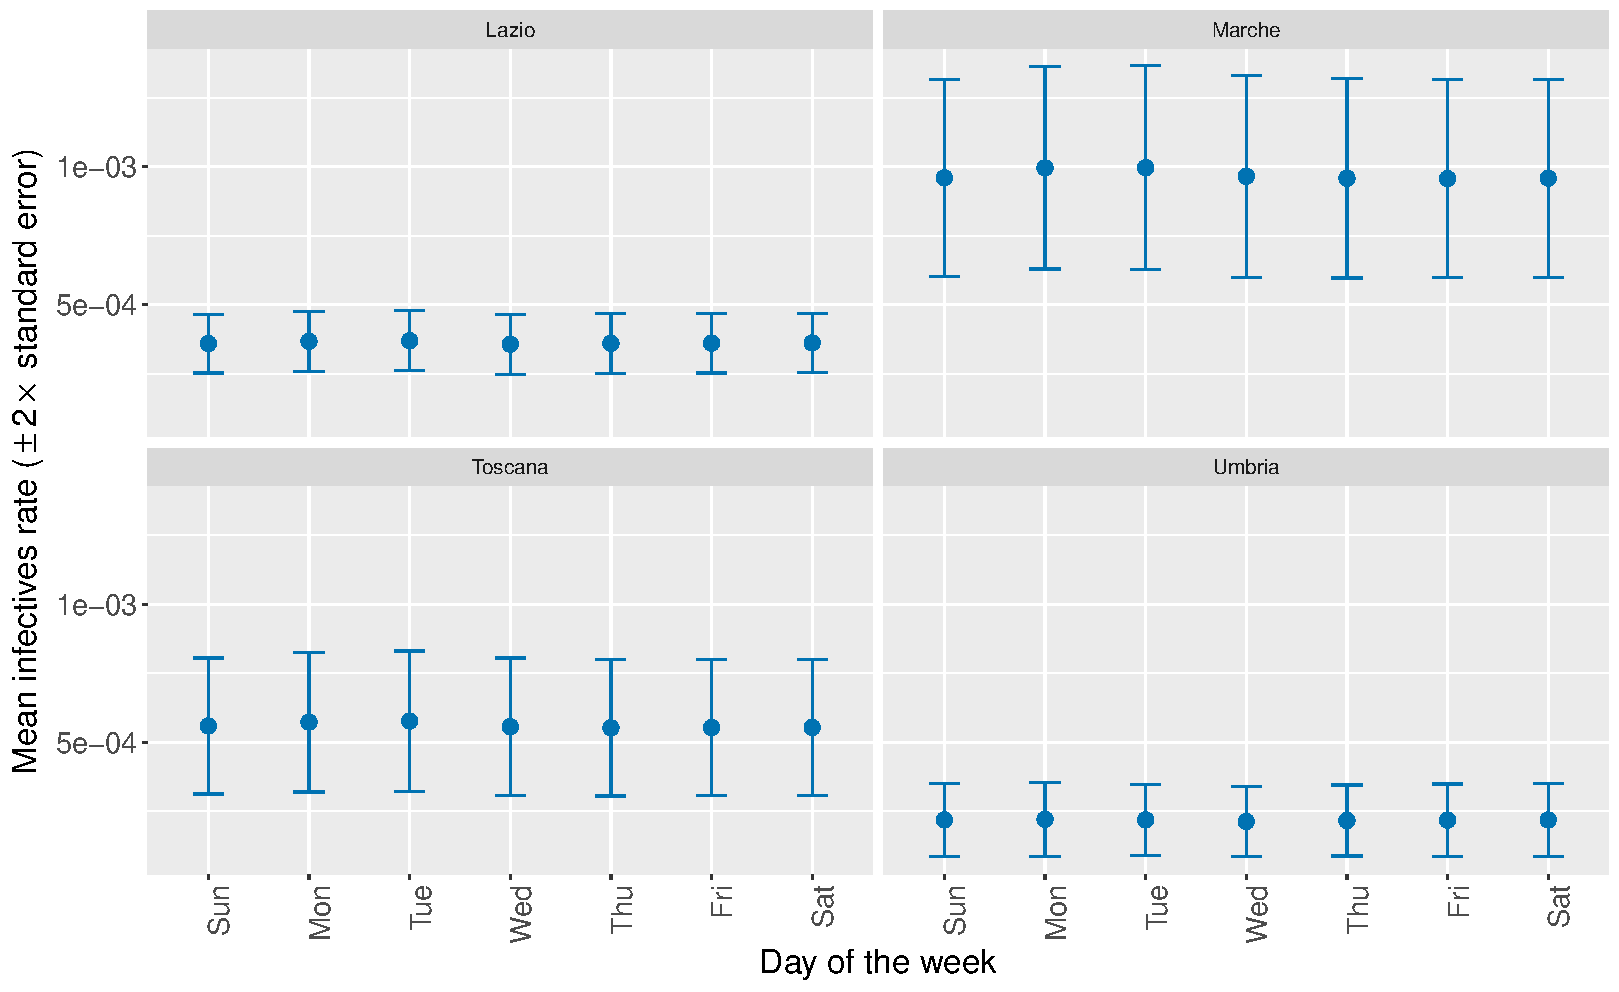
\includegraphics[width=0.98\textwidth]{output/infective_rates_weekday_Centro (IT).pdf}
	    \caption{Incidence rate per NUTS 2 region per day of the week for the \textit{Centro (IT)} (Centre) NUTS 1 region}
	    \label{fig:incidence_Centro_weekday}
	\end{figure}
	
	Figure \ref{fig:incidence_Centro_weekday} shows us that, although the mean incidence rate for Sunday is usually the highest, there is no statistical evidence to infer that there is a higher incidence rate on certain days. This can be concluded because the given error bars of two times the standard deviation overlap. As such, our intuition is likely not as strong on this subject. Nonetheless, we include the variable in the model because an inspection in isolation is not necessarily an indication that the variable is not predictive for the intended dependent variable.
	
	\newpage
	\section{Methodology} \label{sec:methodology}
	In this section, we discuss our models and the thought process behind them. In Section \ref{sec:sir_model}, we describe the most commonly used model in epidemiology: the SIR model. In Section \ref{sec:model_within}, we present a model ignoring effects across regions and for which the transmission rate parameter is determined by the previous infectives. Subsequently, Section \ref{sec:model_within_between} presents a model that takes effects across regions into account for which the transmission rate parameter is determined by the previous infectives. Having discussed the models presented by \textcite{adda2016economic}, we consider how to do model selection for these two models to determine the best set of regressors to use in Section \ref{sec:model_selection}. After this, we develop our own discrete SIR model in Section \ref{sec:discrete_sir_model}, which is estimated by panel data methods and Bayesian estimation. Lastly, Section \ref{sec:undocumented_modelling} describes how undocumented infectives are modelled.
	
	\section{The SIR model}\label{sec:sir_model}
	In this section, we explain the most commonly used model in epidemiology, namely the Standard Inflammatory Response (SIR) model \parencite{kermack1927contribution, anderson1992infectious}. We follow the notation by \textcite{keeling2011modeling} throughout this thesis. The SIR model splits the total population into three groups. $S$ denotes the fraction of individuals who are susceptible to being infected, $I$ denotes the fraction of individuals who are currently infected, also called infectives, and $R$ denotes the fraction of individuals who have been removed from the model, be that because they successfully recovered from the disease or because they have deceased. We furthermore define $s$ to be the number of susceptible individuals, $i$ to be the number of infectives, and $r$ to be the number of recovered individuals, so that $S = s/N$, $I = i/N$, and $R = r/N$, where $N$ is the total population size. As such, at any point in time, we have that
	\[S,I,R \in [0,1] \text{ and } S+I+R=1.\]
	\[s,i,r \in [0,N] \text{ and } s+i+r=N.\]
	
	The SIR model makes four main assumptions. Understanding these assumptions also tell us how the model is constructed. The first assumption is that the population is constant, meaning that births and deaths are ignored. The second assumption that is made under the SIR model is that there is a time-constant rate of change in infectives. This rate is proportional to the interaction between the infectives and the susceptible population. In equations \eqref{eq:SIR_model_S}, \eqref{eq:SIR_model_I}, \eqref{eq:SIR_model_X}, and \eqref{eq:SIR_model_Y}, this is represented by the parameter $\beta$, also called the \textit{transmission term} or the \textit{force of infection} \parencite{keeling2011modeling}.
	\todo[inline]{Q: Can I reference equations before they are presented or should I remove these references?}
	The third assumption that the SIR model makes is that there is a constant rate of change at which infectives recover or decease. This is represented by the recovery rate $\gamma$ in equations \eqref{eq:SIR_model_I}, \eqref{eq:SIR_model_R}, \eqref{eq:SIR_model_Y}, and \eqref{eq:SIR_model_Z}. \todo{Q: Dito} \\
	
	Finally, we assume that there is a constant rate of change at which immune individuals lose their immunity. This is denoted by the parameter $\omega$ in equations \eqref{eq:SIR_model_S}, \eqref{eq:SIR_model_I}, \eqref{eq:SIR_model_X}, and \eqref{eq:SIR_model_Z}. \todo{Q: Dito} For instance, \textcite{adda2016economic} mentions that $\omega$ is set to 0 for chickenpox as individuals acquire a lifetime immunity while $\omega$ will be high for gastroenteritis due to almost no immunity emerging. In the case of COVID-19, some studies show that it is likely that individuals who recovered from COVID-19 may be immune to reinfection, at least temporarily \parencite{kirkcaldy2020covid}. This can be challenged because it is currently still unknown whether immunity is always achieved, especially among those who have had only light to medium symptoms. However, it is estimated that COVID-19 antibodies will remain in a patient’s system for two to three years, based on what is known about other coronaviruses but it is too early to know for certain \parencite{leung_2020}. However, it has recently become clear that reinfection is indeed possible. Two Chinese persons have been tested positive in August after having recovered from COVID-19 a few months prior \parencite{bloomberg2020reinfection}. Therefore, future research could be done to incorporate this new information but this thesis assumes that, for simplicity's sake, we assume that lifelong immunity is achieved, or at least long enough to last through the temporal scope of our analysis: we set $\omega = 0$. \\
	
	Now that the assumptions from the SIR model is clear, we present the definition of the SIR model. The SIR model is postulated in continuous time, i.e. the equations in \eqref{eq:SIR_model_S}, \eqref{eq:SIR_model_I}, and \eqref{eq:SIR_model_R} depict the change in the variables $S$, $I$, and $R$, respectively, for one time period ahead.
	
	\begin{align}
    	\frac{dS}{dt} &= -\beta SI + \omega R, \label{eq:SIR_model_S}\\
    	\frac{dI}{dt} &= \beta SI - \gamma I, \label{eq:SIR_model_I}\\
    	\frac{dR}{dt} &= \gamma I - \omega R. \label{eq:SIR_model_R}
	\end{align}
	
	This type of model is also called a stock-and-flow model because there is a certain stock at some point in time (for instance the number of infectives) to which a flow is added and/or subtracted. \textcite{keeling2011modeling} state that the SIR model can also be described by density-dependent transmission instead of frequency-dependent transmission. By that, they mean that the variables $s$, $i$, and $r$ are used instead of $S$, $I$, and $R$. This is given by:
	
	\begin{align}
    	\frac{dX}{dt} &= -\beta si + \omega r, \label{eq:SIR_model_X}\\
    	\frac{dY}{dt} &= \beta si - \gamma i, \label{eq:SIR_model_Y}\\
    	\frac{dZ}{dt} &= \gamma i - \omega r. \label{eq:SIR_model_Z}
	\end{align}
	
	One of the main measures resulting from the SIR model is the estimation of the effective reproduction number $R_{eff} \coloneqq \beta / \gamma$. An epidemic is said to develop if $R_{eff} > 1$. This is clear because $R_{eff} > 1$ implies that $\beta > \gamma$, i.e. the spread of the virus exceeds the recovery rate: individuals in a society become infected more quickly than they recover. The reproduction number $R_{eff}$ is widely used to indicate whether an ongoing epidemic is dying out. For instance, the Italian health ministry has posted an article on May 9, 2020 to communicate that the $R_0$, being the basic reproduction rate, for COVID-19 was below 1 in Italy, at between 0.5 and 0.7 \parencite{saluteR0}.
	
	\section{Within-Region Spread Model} \label{sec:model_within}
	In this section, we present the stripped down model by \textcite{adda2016economic} ignoring effects across regions. Recall that the SIR model is postulated in continuous time. \textcite{adda2016economic} provides a discrete-time model that seems to be based on the SIR model. \textcite{adda2016economic} does not discuss how the discretization is carried out. Therefore, we discuss how the discretization appears to be carried out. Recall from \eqref{eq:SIR_model_I} that $\frac{dI}{dt} = \beta SI - \gamma I$. As such, the discretized version (for a region $r$) is:
	    \begin{equation}\label{eq:discretized_sir}
	        I_{r,t} - I_{r,t-1} = \beta S_{r,t-1}I_{r,t-1} - \gamma I_{r,t-1}.
	    \end{equation}
	   
	There are a few things to note. Firstly, if we want to estimate this equation's parameters, an error occurs. This is added to the model through an error term denoted by $\eta_{r,t}$:
	    \begin{equation}\label{eq:discretized_sir_error}
	        I_{r,t} - I_{r,t-1} = \beta S_{r,t-1}I_{r,t-1} - \gamma I_{r,t-1} + \eta_{r,t}.
	    \end{equation}
	
	Secondly, individuals that get infected do not immediately infect others because there is a so-called latent period, which is the period between an infection and the moment that the infective is infectious. For COVID-19, the latent period is estimated to be approximately 2 days shorter than the incubation period \parencite{he2020temporal}. The incubation period is the period between an infection and the moment that the infected individual starts showing symptoms, at which point the infective is said to be symptomatic. The incubation period for COVID-19 is estimated to be above 2 and below 11.5 \parencite{lauer2020incubation}, 12.5 \parencite{li2020incubation}, or 14 days \parencite{linton2020incubation}. This is a large range, but this is not rare. For instance, the incubation period for chicken pox is estimated to be between 9 and 21 days \parencite{papadopoulos2018chickenpox}. While the maximum incubation period is not agreed upon by \textcite{lauer2020incubation} and \textcite{li2020incubation}, their results on the median are similar. \textcite{lauer2020incubation} report a median incubation period of 5.1 days (95\% CI: 4.5 to 5.8 days), while \textcite{li2020incubation} report a median incubation period of 5.2 days (95\% CI: 4.1 to 7.0 days). For comparison, \textcite{linton2020incubation} give the result of a mean incubation period of 5.0 days (95\% CI: 4.2 to 6.0 days) when excluding Wuhan residents and 5.6 days (95\% CI: 5.0 to 6.3 days) when including Wuhan residents. \\
	
	Because the latent period is estimated to be shorter than the incubation period, there are infectives who are able to infect others before showing symptoms. We call these people pre-symptomatic, which is distinctive from asymptomatic people in the sense that asymptomatic people do not develop symptoms and pre-symptomatic people will develop symptoms but they develop a higher viral load just before said symptoms are apparent. On June 9, 2020, the World Health Organization said that it is unclear whether asymptomatic people can actually spread the virus but that pre-symptomatic people may actually be able to infect others \parencite{bloomberg2020AsymptomaticSpread}. This may be an issue when considering policies such as self-isolation when one is sick, because an infective may have already spread the virus before feeling sick. \textcite{bloomberg2020AsymptomaticSpread} moreover reiterate the WHO's statement that studies have been done that show that asymptomatic people can spread the virus but that more research needs to be done to show how many of these infectious asymptomatic people exist. We discuss how we model pre-symptomatic individuals in Section \ref{sec:undocumented_modelling}. \\
	
	\textcite{adda2016economic} models the transmission lag by making the lag on the right hand side of \eqref{eq:discretized_sir_error} dependent on the incubation period. This is denoted by the parameter $\tau$:
	    \begin{equation}\label{eq:discretized_sir_tau}
	        I_{r,t} - I_{r,t-1} = \beta S_{r,t-\tau}I_{r,t-\tau} - \gamma I_{r,t-\tau} + \eta_{r,t}.
	    \end{equation}
	
	For instance, \textcite{adda2016economic} chooses $\tau$ equal to one week for acute diarrhea and flu-like illnesses as these have an incubation period of less than a week. Due to the results from \textcite{lauer2020incubation}, \textcite{li2020incubation}, and \textcite{linton2020incubation}, indicating an incubation period for COVID-19 of roughly five days, and the result from \textcite{he2020temporal} that the latent period is roughly two days shorter than the incubation period, we choose $\tau = 3$. \\
	
	\textcite{adda2016economic} adds regressors to the model as control variables, such as the region fixed effects, week effects and year effects in levels. Note that regressors can be added to the model to capture possible effects that would otherwise be included in the error, confounding the estimation of the transmission parameter $\beta$. \textcite{adda2016economic} denotes this tensor of regressors by $X$, not to be confused with the notation by \textcite{keeling2011modeling} for the number of infectives. This leads to the following formulation:
	    \begin{equation}\label{eq:discretized_sir_regressors}
        	I_{r,t} - I_{r,t-1} = \beta S_{r,t-\tau}I_{r,t-\tau} - \gamma I_{r,t-\tau} + \delta X_{r,t} + \eta_{r,t}.
    	\end{equation}
    	
	For our application, the data does not span multiple years. As such, we do not have year effects. Also note that week effects would capture a time trend because we do not have the same week number multiple times for the same region. Therefore, we will not include a week effect. We do add a weekend effect. More information and reasoning is provided in Section \ref{subsec:regressor_data}. \\
	
	There are two other key differences in the model specification by \textcite{adda2016economic} compared to \eqref{eq:discretized_sir_regressors} that are not clear from the paper. First of all, \textcite{adda2016economic} replaces the incidence rate $I_{r,t-\tau}$, also called the incidence rate, by the number of new cases $i_{r,t-\tau} - i_{r,t-\tau-1}$. Similarly, \textcite{adda2016economic} puts the dependent variable to be the number of new cases instead of the incidence rate. Second of all, \textcite{adda2016economic} does not include the term $\gamma I_{r,t-\tau}$ in the model. Presumably, this is because \textcite{adda2016economic} considers the number of new cases instead of the total number of infectives and, therefore, the number of recovered individuals do not impact that value. In this section and Section \ref{sec:model_within_between}, we will continue with this model to see how the models perform in the case of COVID-19. Even though the mathematical derivation of the model does not explicitly derive from the SIR model, it may still provide correct estimates. \\
	
	Now we present the final model, ignoring effects across regions, by \textcite{adda2016economic}. Defining $\Delta i_{r,t} \coloneqq  \coloneqq i_{r,t} - i_{r,t-1}$ and following the notation by \textcite{keeling2011modeling}, the within-region model is given by:
	\begin{equation} \label{eq:model_within}
	    \Delta i_{r,t} = \beta_{within}S_{r,t-\tau}\Delta i_{r,t-\tau} + \delta X_{r,t} + \eta_{r,t}
	\end{equation}
	
	The model is estimated by ordinary least squares (OLS). The moment condition that needs to be satisfied due to the strict exogeneity assumption is
	    \[E\left[ \eta_{r,t} \left( \beta_{within}S_{r,t-\tau}\Delta i_{r,t-\tau} + \delta X_{r,t} \right) \right] = 0.\]
	
	A general assumption that is made, is that the idiosyncratic error $\eta_{r,t}$ is uncorrelated with the regressors in the tensor $X_{r,t}$. That is, we assume that $E\left[\eta_{r,t} \,\middle|\, X_{r,t}\right] = 0$. Now note that we need to only consider the relation between $\eta_{r,t}$ and $S_{r,t-\tau}\Delta i_{r,t-\tau}$. The reason why we assume that $E\left[\eta_{r,t} \,\middle|\, S_{r,t-\tau}\Delta i_{r,t-\tau}\right] = 0$ is that, for a large enough lag $\tau$, the error is not correlated with past data at that lag. That is, the people that are classified as infectives at time $t-\tau$ do not have an effect on the error that we make when considering the infectives at time $t$ under a correct model specification. As such, we assume that the moment condition holds.
	
    \subsection{Results} \label{subsec:results_within}
	In this section, we present the results for the within-region spread model. Firstly, we present the results where the data is pooled to a national level. Subsequently, results are presented for the models per region to which model selection is applied with the Akaike Information Criterion (AIC). For both result sets, we present the results from the regular model as well as modelling the undocumented infectives with a quadratic form with $\gamma = 0.7$ and $f^{min} = 0.1$ as in \eqref{eq:quadratic_functional_form}. \\
	
	For all models, we apply a rolling window of 100 days, meaning that the used data spans May 9 till August 16. The reason behind this is that infections from the past should not dominate the latest estimates of the transmission rate parameters. When the (first) wave has passed and the transmission rate is low, including the data from during the peak moment of the pandemic will influence the transmission rate. We will illustrate this at the end of the section. \\
	
	Naively, one could consider constructing a model for the entire nation of Italy. Even though this does not take into account regional differences, as described in Section \ref{sec:problem_description}, it may achieve good results if regions are sufficiently similar. However, as we have already seen in Section \ref{sec:problem_description}, there is indeed a difference among regions and pooling the data is likely not a good solution. The results from estimating \eqref{eq:model_within} with OLS for the national data are given in Table \ref{tab:results_within_national}. Model selection with AIC is not applied.
	
	\begin{longtable}{@{}lrrrlrrrl@{}}
		\caption{Estimates from Within-Region Spread Model on a national level. Data spans May 9 till August 16, 2020 (100 days). Undocumented infectives are modelled using the quadratic specification with $\gamma = 0.7$ and $f^{min}=0.1$.}
		\label{tab:results_within_national}\\
		\toprule
		& \multicolumn{4}{c}{Regular model} & \multicolumn{4}{c}{Modelling undocumented infectives} \\
		                \cmidrule(lr){2-5}
                        \cmidrule(lr){6-9}
		& Estimate & Std. Error & $t$ value & $p$ value & Estimate & Std. Error & $t$ value & $p$ value \\* \midrule
		\endfirsthead
		
		\multicolumn{9}{c}{{\bfseries Table \thetable\ continued from previous page}} \\
		\toprule
		& \multicolumn{4}{c}{Regular model} & \multicolumn{4}{c}{Modelling undocumented infectives} \\
		                \cmidrule(lr){2-5}
                        \cmidrule(lr){6-9}
		& Estimate & Std. Error & $t$-value & $p$-value & Estimate & Std. Error & $t$-value & $p$-value \\* \midrule
		\endhead
		
		\bottomrule
		\multicolumn{9}{c}{{\bfseries Table \thetable\ continues on next page}}
		\endfoot
		
		\multicolumn{9}{c}{Significance levels: * = 0.1 ** = 0.05, *** = 0.01}
		\endlastfoot
		
		Weekend             & 11.6035 & 31.4783 & 0.369 & 0.713    & 36.761 & 141.003 & 0.261 & 0.795 \\*
		$\beta_{within}$    & 0.886 & 0.041 & 21.493 & 0.000*** & 0.863 & 0.036 & 23.925 & 0.000*** \\* \bottomrule
	\end{longtable}
	
	Table \ref{tab:results_within_national} shows estimates for $\beta_{within}$ of 0.886 and 0.863 for the models excluding and including undocumented infections, respectively. Both estimated parameters are statistically significant at a 1\% significance level, whether undocumented infectives are modelled or not. As mentioned earlier in this section, this model does not take into account effects specific to regions. It is also clear that the same model might not be suitable for all regions; we should apply model selection to the individual models as was explained in Section \ref{sec:model_selection}. To execute model selection, we use the AIC and we make sure that the term for $\beta_{within}$ remains in the model, meaning that model selection is solely performed on whether the weekend dummy should be included. In Table \ref{tab:results_within_aic}, we present the results. In Table \ref{tab:results_within} in Appendix \ref{app:tables}, we present the results from running the model on each region separately with the same model specification for each region. The results comparing the use of the BIC over the AIC for model selection are presented in Table \ref{tab:model1_aic_vs_bic}, where we see that the BIC selects a smaller model for three regions, being Marche, Apulia, and Veneto, but that the model specification is the same for all of the other regions.
	
	\begin{longtable}{@{}lcccc@{}}
		\caption{Estimates from Within-Region Spread Model per region with model selection by AIC. Estimates are given with $t$-statistics in parentheses. Data spans May 9 till August 16, 2020 (100 days). Undocumented infectives are modelled using the quadratic specification with $\gamma = 0.7$ and $f^{min}=0.1$.}
		\label{tab:results_within_aic}\\
		\toprule
		                & \multicolumn{2}{c}{Regular model} & \multicolumn{2}{c}{Modelling undocumented infectives} \\
		                \cmidrule(lr){2-3}
                        \cmidrule(lr){4-5}
		Region          & $\beta_{within}$ & Weekend & $\beta_{within}$ & Weekend \\* \midrule
		\endfirsthead
		
		\multicolumn{5}{c}{{\bfseries Table \thetable\ continued from previous page}} \\
		\toprule
		                & \multicolumn{2}{c}{Regular model} & \multicolumn{2}{c}{Modelling undocumented infectives} \\
		                \cmidrule(lr){2-3}
                        \cmidrule(lr){4-5}
		Region          & $\beta_{within}$ & Weekend & $\beta_{within}$ & Weekend \\* \midrule
		\endhead
		
		\bottomrule
		\multicolumn{5}{c}{{\bfseries Table \thetable\ continues on next page}}
		\endfoot
		
		\multicolumn{5}{c}{Significance levels: * = 0.1 ** = 0.05, *** = 0.01}
		\endlastfoot
		
        National & 0.893*** & & 0.867*** &  \\ 
         & (24.665) & & (26.564) &  \\ 
        ABR & 0.463*** & 2.715** & 0.494*** & 12.934** \\ 
         & (5.081) & (2.084) & (5.854) & (2.160) \\ 
        BAS & 0.089 &  & 0.095 &  \\ 
         & (0.868) &  & (0.933) &  \\ 
        BZ & 0.460*** & 2.111*** & 0.386*** & 6.531*** \\ 
         & (5.172) & (3.566) & (4.541) & (3.819) \\ 
        CAL & 0.297*** & 2.176** & 0.269** & 12.544*** \\ 
         & (2.689) & (2.600) & (2.499) & (2.755) \\ 
        EMR & 0.737*** & 14.644*** & 0.703*** & 54.997*** \\ 
         & (13.514) & (3.441) & (14.736) & (3.329) \\ 
        FVG & 0.719*** & 1.106 & 0.772*** &  \\ 
         & (9.005) & (1.465) & (12.629) &  \\ 
        LAZ & 0.840*** & 6.783*** & 0.795*** & 38.587*** \\ 
         & (13.863) & (2.705) & (13.695) & (2.712) \\ 
        LIG & 0.811*** &  & 0.828*** &  \\ 
         & (14.233) &  & (16.459) &  \\ 
        LOM & 0.805*** &  & 0.783*** &  \\ 
         & (14.701) &  & (14.183) &  \\ 
        MAR & 0.576*** & 2.297* & 0.572*** & 11.050** \\ 
         & (7.693) & (1.836) & (9.102) & (2.055) \\ 
        MOL & 0.351*** & & 0.348*** &  \\ 
         & (6.979) &  & (8.064) &  \\ 
        PIE & 0.807*** &  & 0.788*** &  \\ 
         & (18.492) &  & (18.917) &  \\ 
        PUG & 0.639*** & 2.023* & 0.586*** & 13.379* \\ 
         & (9.129) & (1.678) & (9.265) & (1.920) \\ 
        SAR & 0.372*** &  & 0.361*** &  \\ 
         & (3.905) & & (3.924) &  \\ 
        TOS & 0.735*** & 6.130*** & 0.702*** & 26.588*** \\ 
         & (10.869) & (3.411) & (11.061) & (3.355) \\ 
        UMB & 0.607*** & 1.094** & 0.506*** & 4.070** \\ 
         & (5.918) & (2.498) & (5.059) & (2.501) \\ 
        VDA & 0.216** & & 0.298*** &  \\ 
         & (2.259) & & (3.346) &  \\ 
        VEN & 0.652*** & 9.808 & 0.652*** & 22.618 \\ 
         & (6.866) & (1.529) & (7.784) & (1.531) \\* \bottomrule
	\end{longtable}

    We first discuss the statistical evidence for the estimated values of $\beta_{within}$, where we start by considering the model excluding undocumented infectives. After this, we will consider the interpretation of the coefficients and the model selection. Considering the estimates of $\beta_{within}$, we see that these differ vastly over the regions with varying degrees of statistical significance. For only one region, we find no statistically significant result, namely Basilicata. For the region of Aosta Valley, the estimate of $\beta_{within}$ is statistically significant at a level of 0.05. For all other regions, the estimates are statistically significant at a level of 0.01. Looking only at the statistically significant estimates, these range from 0.216 for Aosta Valley till 0.893 for the national model. Excluding the national model, the highest estimate $\beta_{within}$ is 0.840 for Lazio. This already shows that a national model is not to be applied to individual regions, despite the statistical significance of the estimate of $\beta_{within}$ for the national model. \\

    If we model undocumented infectives, we again see that no statistical evidence is found for the estimated transmission rate for Basilicata. For all other regions, including Aosta Valley, the estimate is statistically significant at a level of 0.01, ranging from 0.269 for Calabria till 0.867 for the national model. Excluding the national model, the highest estimate is 0.828 for the region of Liguria. Therefore, modelling undocumented infectives does mean that the order of magnitude between the regions can differ. Whereas Lazio has the second-highest estimate for the case when undocumented infectives are not modelled, this is now the case for Liguria. We also see that the estimates generally differ a bit from the ones discussed previously, though not immensely in the sense that a high value is suddenly very low. Including the national model as well as the statistically insignificant estimates, the estimate is higher in 26.3\% of the cases (five out of nineteen) and lower in the other 73.7\%. As such, there is no consistent effect of the modelling method used that biases the results in one typical direction. \\

    When we want to interpret the estimates of $\beta_{within}$, we should recall that \textcite{adda2016economic} notices that these can be interpreted as the marginal effects of a change in the infection rate on the future infection rate when the entire population is susceptible to the disease. However, notice that this is made with the model formulation as explained in Section \ref{sec:model_within}, where the removal term is omitted from the model. Because this does not take into account the specific removal rate of COVID-19, we cannot interpret the coefficients in the same way. However, we can compare the magnitude of the coefficients with one another. For instance, let us compare the regions of Lombardy and the island of Sardinia. We consider the model where undocumented infectives are modelled. For this model, we find estimates of $\beta_{within}$ of 0.783 and 0.361, respectively. Although this cannot tell us much about the spread within the region as explicitly, this does show us that the transmission in Lombardy was much higher than on Sardinia. A similar interpretation can be applied to any comparison of regions and for the model without modelling undocumented infectives. \\

    Regarding the model selection, we indeed see that the AIC gives a varying model selection per region. However, the set of regressors that is used is generally the same whether undocumented infectives are modelled are not. The only exception that we see if for the region of Friuli Venezia Giulia; when excluding undocumented infectives, the weekend dummy is included in the model, whereas it is excluded when undocumented infectives are modelled. We do see that four of the estimates for the weekend dummy's parameter are not statistically significant at a level of 0.05 when we do not model undocumented infectives. When undocumented infectives are modelled, the result for the region of Marche becomes statistically significant but all other regional results retain the same significance level. As mentioned in Section \ref{sec:model_selection}, this is because the AIC tends to select a larger model. When not modelling undocumented infectives, the entire model is selected for eleven out of nineteen regions, and, in the other eight cases, the weekend dummy is excluded. As explained before, the model including undocumented infectives therefore selects the entire model for one region less, so ten out of nineteen cases. \\
	
	We are also interested in looking at the estimate of $\beta_{within}$ over time. That is, if we keep adding data, do we see an interesting effect in its progression? Hopefully, it decreases over time, implying that SARS-CoV-2 is transmitted less. This would support the findings in Figures \ref{fig:incidence_per_NUTS1} and \ref{fig:incidence_Centro}. In Figure \ref{fig:beta_within_over_time_nordest}, we present plots for the regions in the \textit{Nord-Est} (North-East) NUTS 1 region. Plots for the other NUTS 1 regions can be found in Appendix \ref{sapp:model1_plots}, which generaslly show similar results. Each point in the graphs in Figure \ref{fig:beta_within_over_time_nordest} is the estimate of $\beta_{within}$ when only the latest 100 data points before that date are used as described at the beginning of this section. In addition, a LOESS (locally estimated scatter plot smoothing) curve with span parameter 0.3 is fit to the data points to give a better insight in the progression over time. \\
	
	\begin{figure}[H]
	    \centering
	    \begin{subfigure}{\textwidth}
	      \centering
	      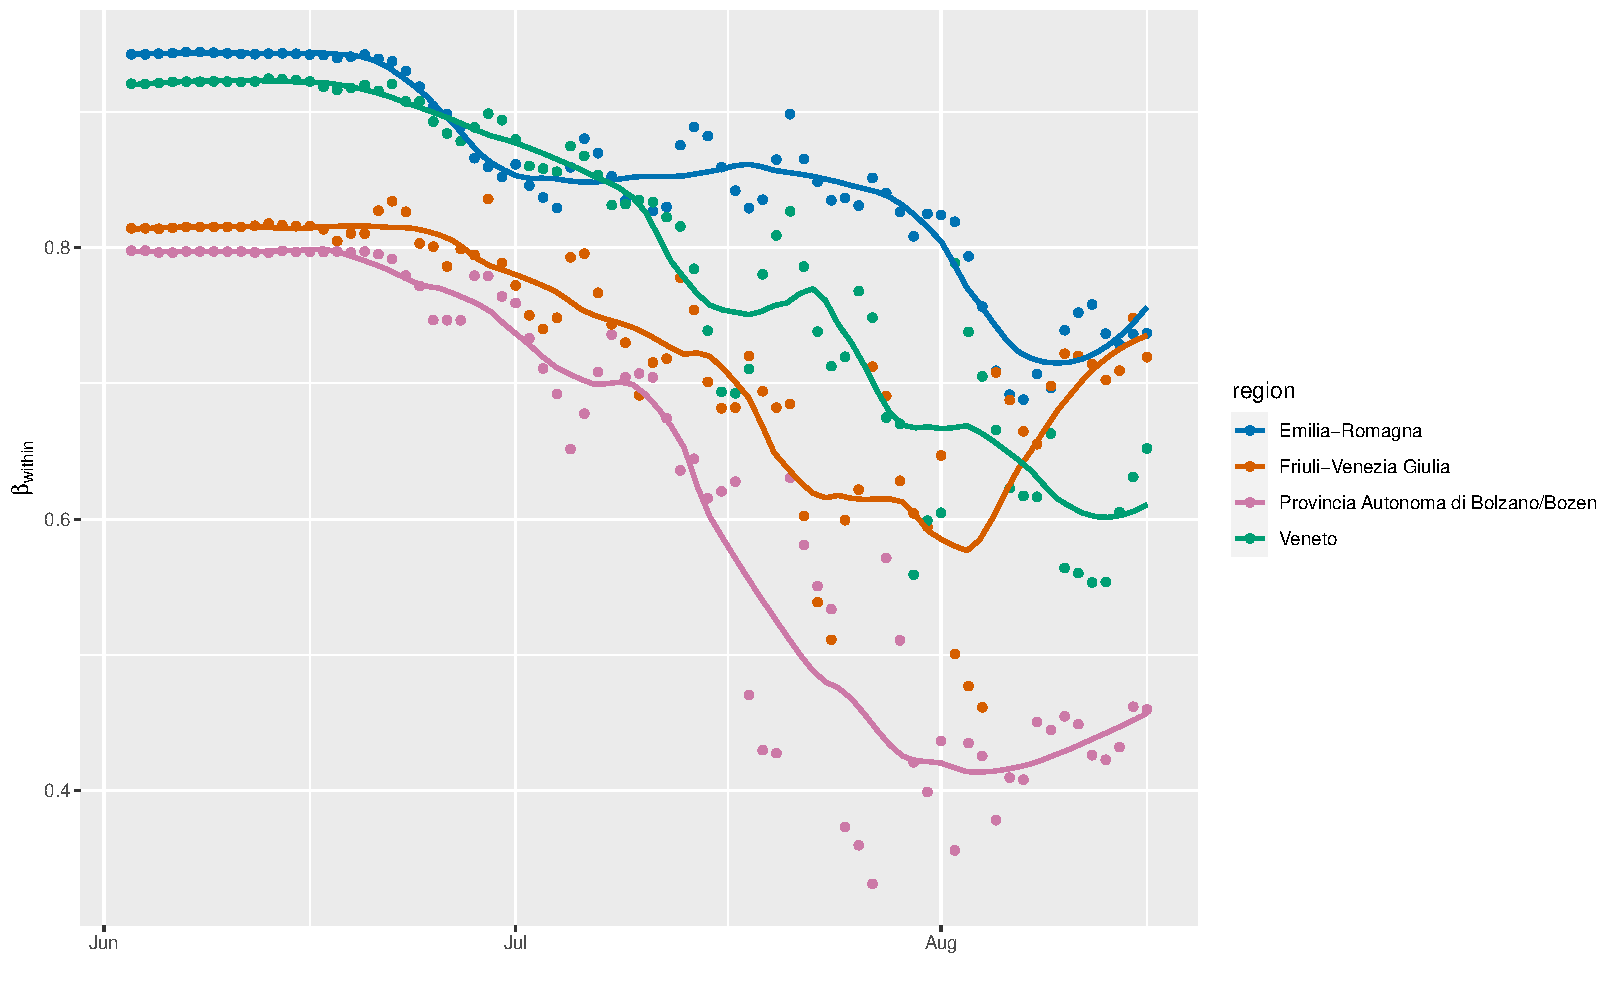
\includegraphics[width=0.95\linewidth]{output/model1_lag3_betawithin_Nord-Est_rolling.pdf}
	      \caption{Without model selection}
	      \label{fig:beta_within_over_time_nordest_regular}
	    \end{subfigure}\newline
	    \begin{subfigure}{\textwidth}
	      \centering
	      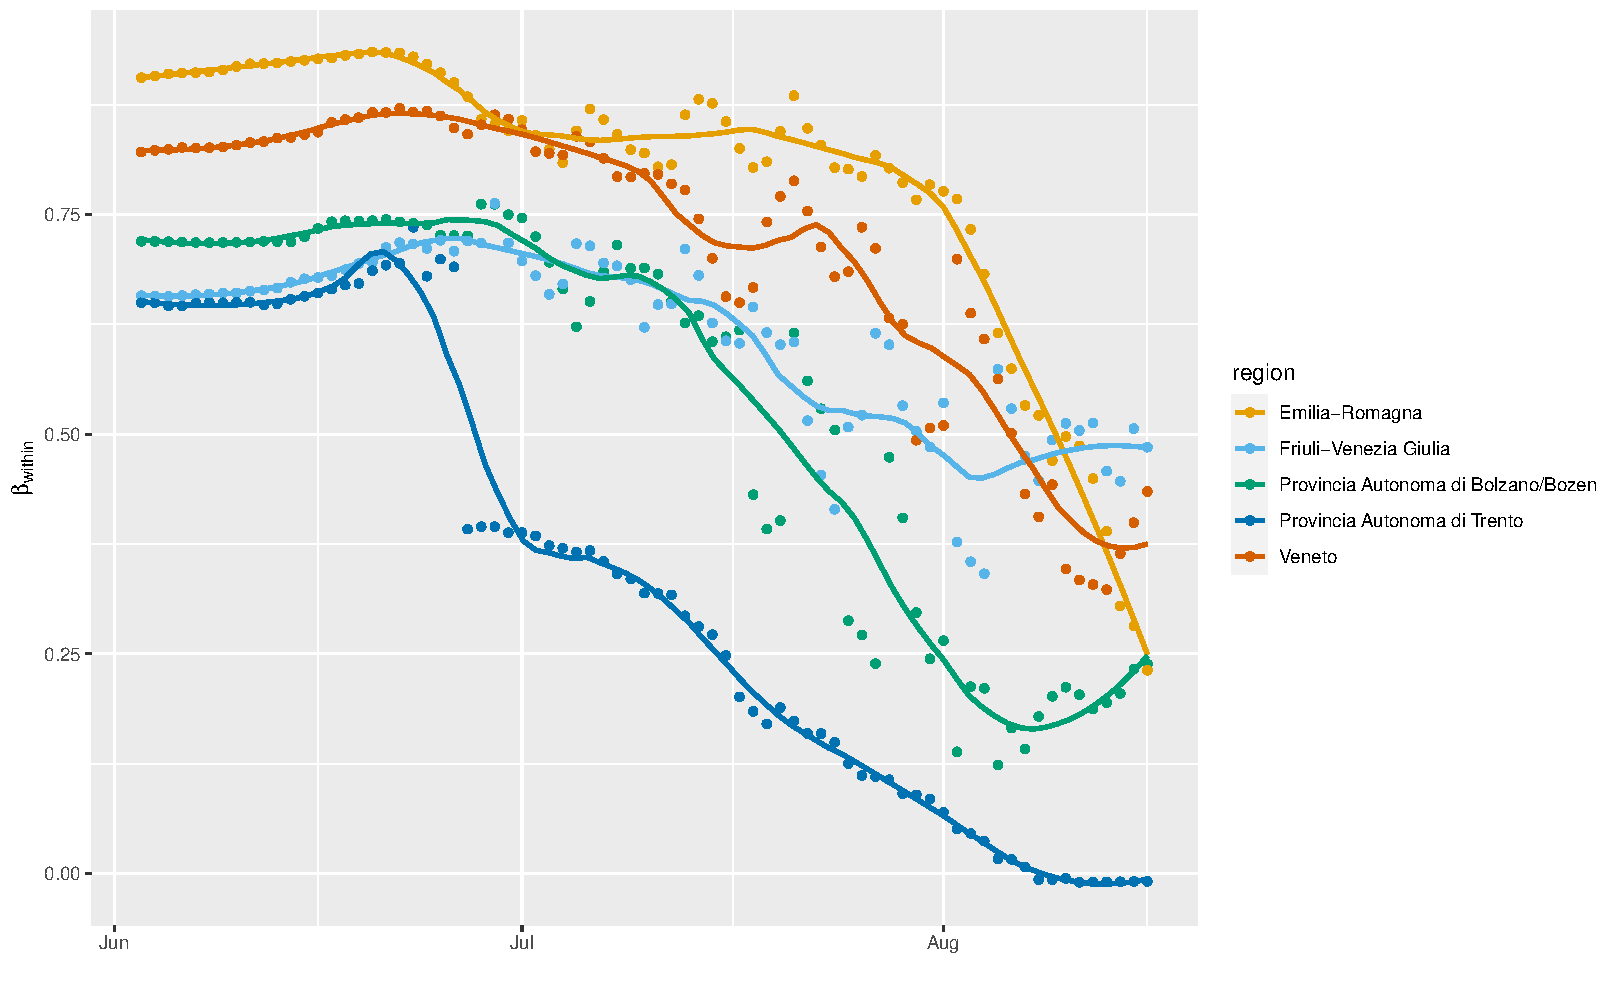
\includegraphics[width=0.95\linewidth]{output/model1_lag3_betawithin_Nord-Est_aic_rolling.pdf}
	      \caption{With model selection by AIC}
	      \label{fig:beta_within_over_time_nordest_aic}
	    \end{subfigure}
	\end{figure}
    \begin{figure}[H]\ContinuedFloat
	    \begin{subfigure}{\textwidth}
	      \centering
	      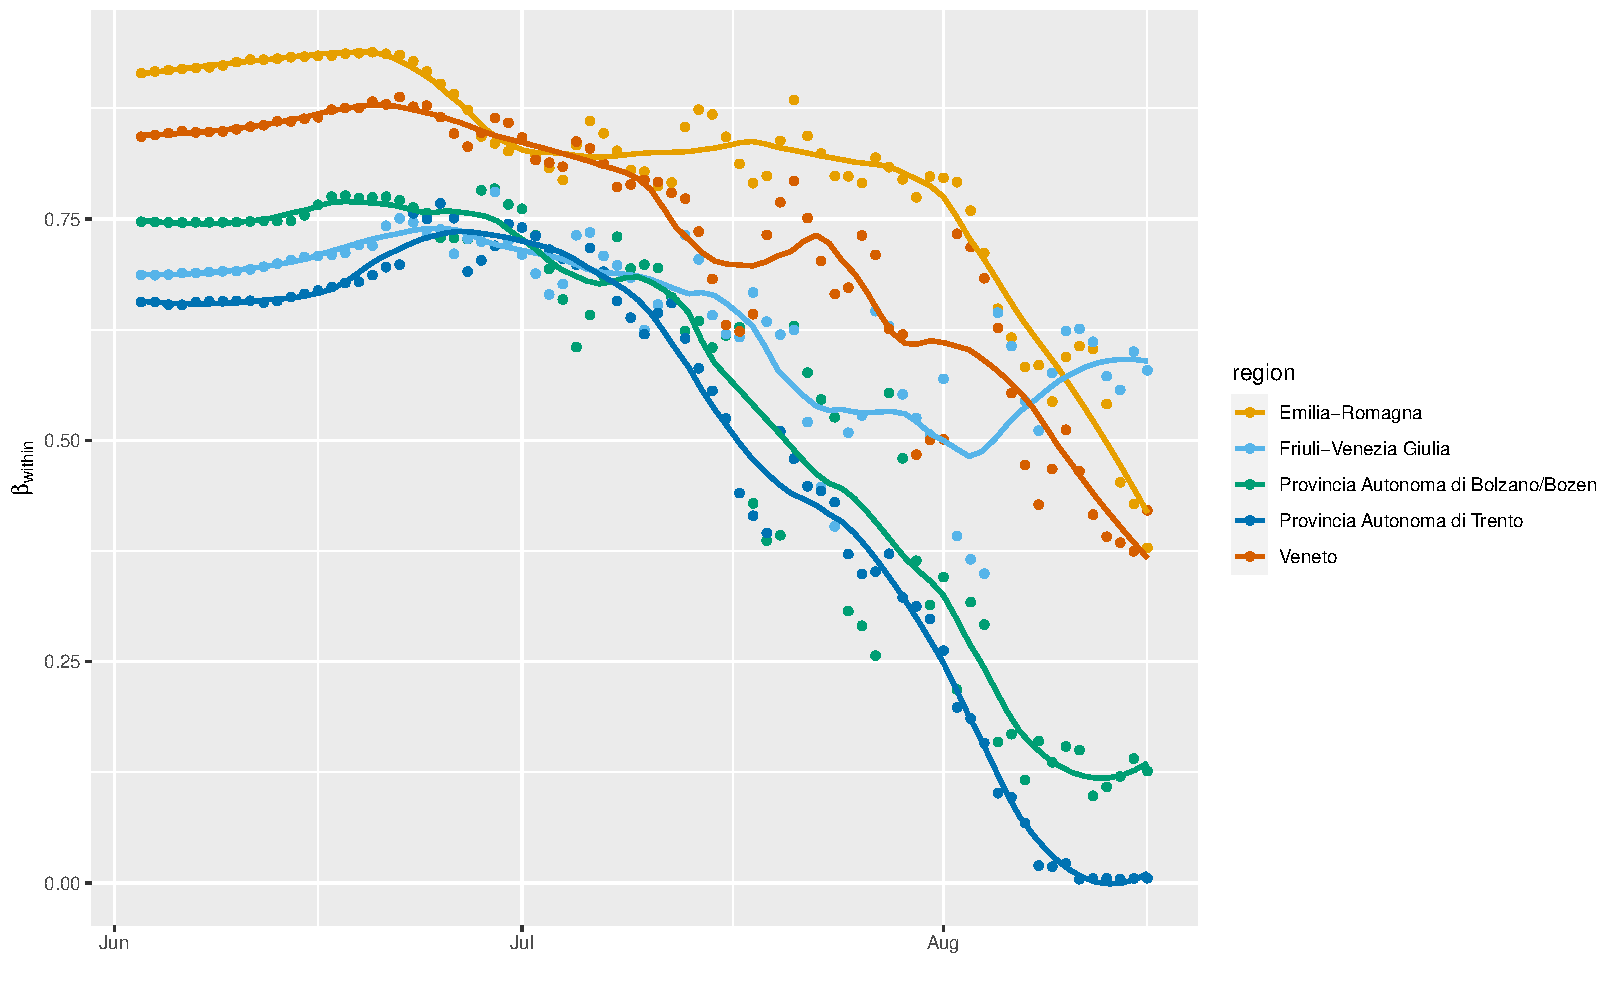
\includegraphics[width=0.95\linewidth]{output/model1_lag3_betawithin_Nord-Est_UndocQuadratic_rolling.pdf}
	      \caption{Without model selection; \\ including undocumented infectives}
	      \label{fig:beta_within_over_time_nordest_regular_undoc}
	    \end{subfigure}\newline
	    \begin{subfigure}{\textwidth}
	      \centering
	      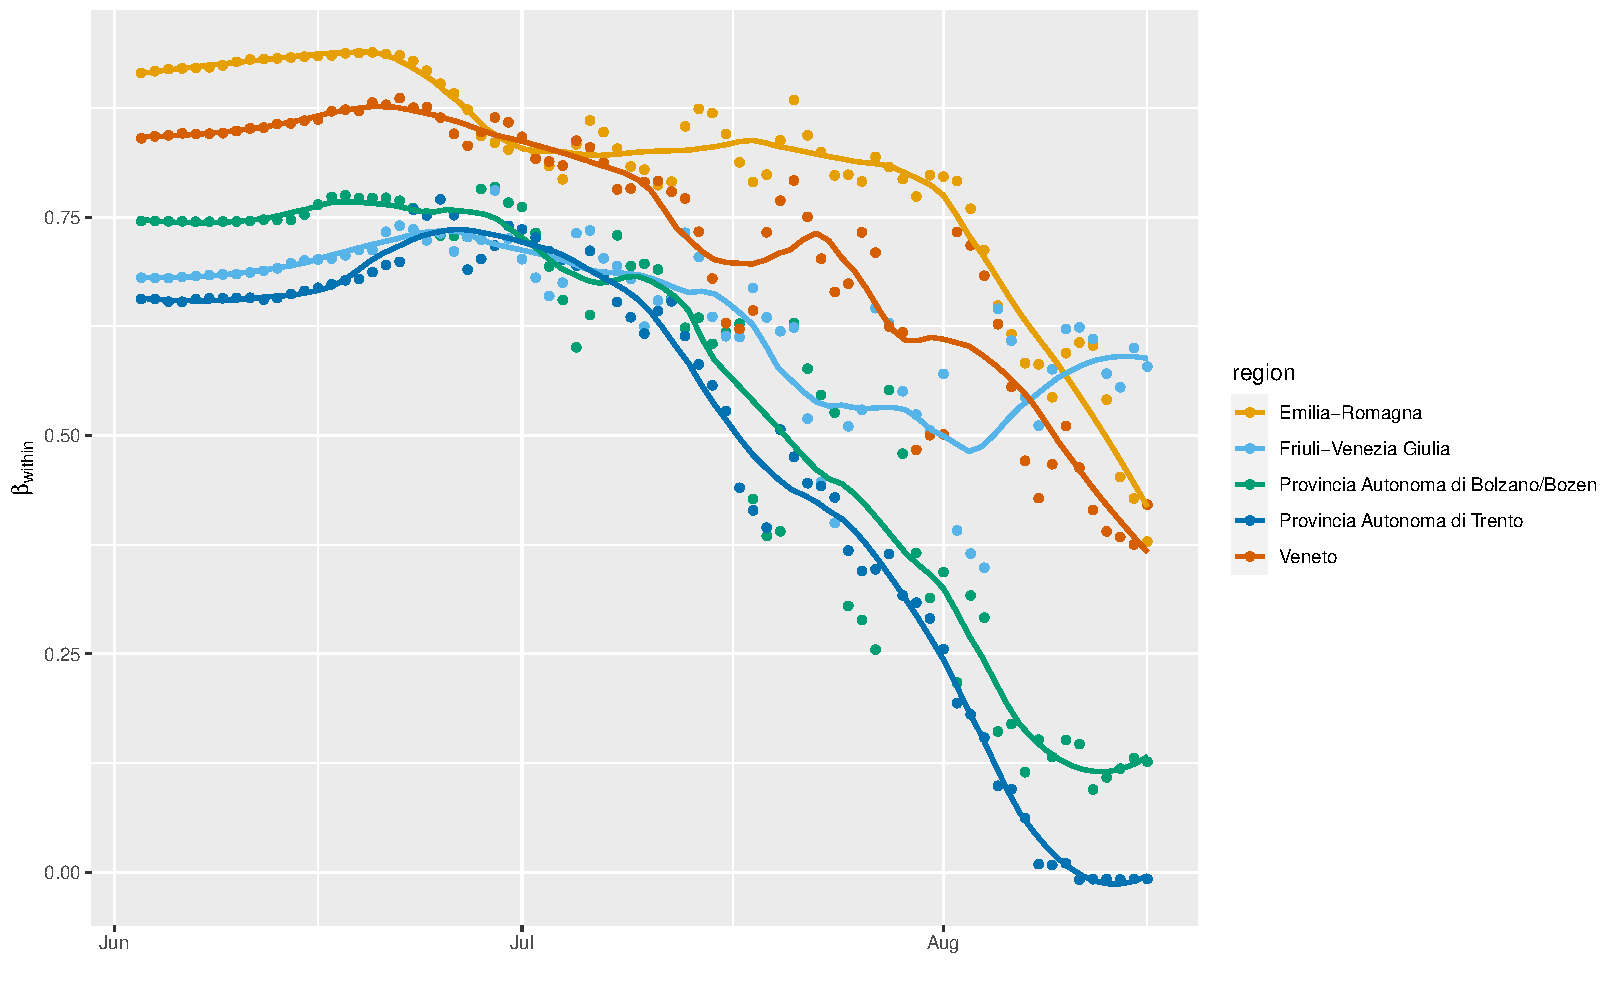
\includegraphics[width=0.95\linewidth]{output/model1_lag3_betawithin_Nord-Est_aic_UndocQuadratic_rolling.pdf}
	      \caption{With model selection by AIC; \\ including undocumented infectives}
	      \label{fig:beta_within_over_time_nordest_aic_undoc}
	    \end{subfigure}
	    \caption{Progression of $\beta_{within}$ over time for the \textit{Nord-Est} (North-East) NUTS 1 region}
	    \label{fig:beta_within_over_time_nordest}
    \end{figure}
	
	At first sight, it may seem like applying model selection does not have an effect on the estimates of $\beta_{within}$. However, a difference can be perceived more clearly when considering the the start of the graphs. When comparing the models with their equivalent version when including undocumented infectives, the effect is more pronounced, especially at the end of the graphs. Considering the progression of $\beta_{within}$ over time, we indeed see that it decreases over time, as we expected. We do see a slight increase in the estimates of $\beta_{within}$ towards the end of the timespan. This is likely because the amount of infectives increased a bit over time again for multiple regions from mid July onward. Please consider the Figures in Appendix \ref{sapp:figures_problem_description}, which indeed illustrate this increase. \\
	
	At the start of this section, we mentioned the application of a rolling window, meaning that the last 100 days of data are used instead of the entire dataset. We noted that this was the case to avoid old data skewing the results. Consider Figure \ref{fig:beta_within_over_time_nordest_not_rolling}, where we present the plot of $\beta_{within}$ over time for the \textit{Nord-Est} NUTS 1 region when a rolling window is not applied. Undocumented infectives are modelled, as before, using the quadratic specification with $\gamma = 0.7$ and $f^{min}=0.1$.
	
	\begin{figure}[H]
	    \centering
        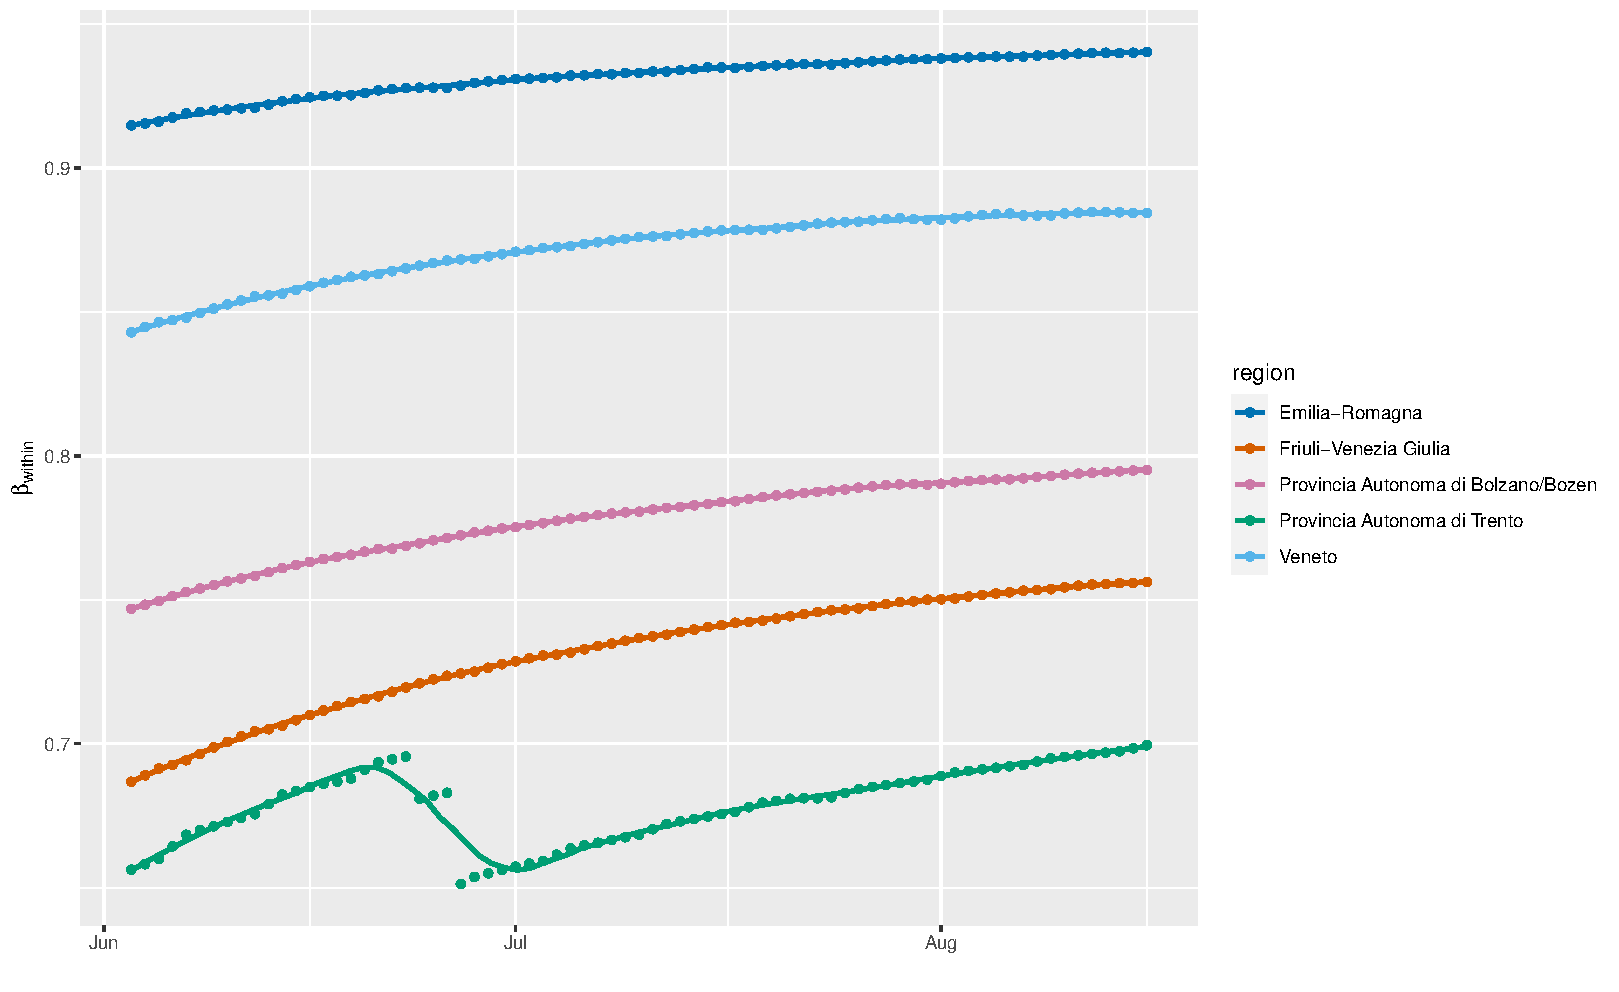
\includegraphics[width=0.95\linewidth]{output/model1_lag3_betawithin_Nord-Est_UndocQuadratic.pdf}
	    \caption{Progression of $\beta_{within}$ over time for the \textit{Nord-Est} (North-East) NUTS 1 region including undocumented infectives without applying a rolling window}
	    \label{fig:beta_within_over_time_nordest_not_rolling}
    \end{figure}
	
	Compare Figure \ref{fig:beta_within_over_time_nordest_not_rolling} with Figure \ref{fig:beta_within_over_time_nordest_regular_undoc}, which applies the same specifications but without applying the rolling window. It is immediately clear that the variation in $\beta_{within}$ is minimal and even slightly increasing. This not intuitive for the reason that a decrease in infectives over time would lead to a lower estimated transmission parameter. As such, it is not logical that the estimate for $\beta_{within}$ would level out over time, especially at a level not close to zero, assuming the pandemic does eventually end. The reason behind choosing 100 days is arbitrary; it is simply a number that retains enough data points while providing variation in the estimates for $\beta_{within}$.
	
	\section{Within and Between-Region Spread Model} \label{sec:model_within_between}
	In this section, we present the model by \textcite{adda2016economic} that takes effects across regions into account. A key addition made by \textcite{adda2016economic} is recognizing that there is spatial spillover between regions. That is, there may be infectives in one region that travel to another region and then infect individuals there. The following model is defined:
	\begin{equation} \label{eq:model_within_between}
	    \Delta i_{r,t} = \beta_{within}S_{r,t-\tau}\Delta i_{r,t-\tau} + \beta_{between}S_{r,t-\tau} \sum_{c \in R \setminus r} \Delta i_{c, t-\tau} + \delta X_{r,t} + \eta_{r,t}
	\end{equation}
	
	Do note that the specification in \eqref{eq:model_within_between} assumes that individuals from all regions are able to meet one another at the same rate. Of course, this assumption is likely not satisfied. Consider, for example, the region of Lombardy, which lies in north-west Italy. Inhabitants of Lombardy are much more likely to travel to bordering regions, such as Piedmont or Veneto, than to regions in the far south, such as Campania or Apulia, or to the islands. As such, it would be better to consider introducing a method by which we only take a certain number of regions that are the closest to another region into account. Another criterion could be to look at economic ties, since SARS-CoV-2 can not only be be transmitted by regular civilians meeting each other but also by the exchange of goods, for example. Nonetheless, in this section, we follow the specification that \textcite{adda2016economic} provides as in \eqref{eq:model_within_between}. \\
	
	The moment condition that needs to be satisfied due to the strict exogeneity assumption is
	    \[E\left[ \eta_{r,t} \left( \beta_{within} S_{r,t-\tau} \Delta i_{r,t-\tau}  + \beta_{between}S_{r,t-\tau} \sum_{c \in R \setminus r} \Delta i_{c, t-\tau} + \delta X_{r,t} \right) \right] = 0.\]
	    
	In the same way as in Section \ref{sec:model_within}, we can assume that $E\left[\eta_{r,t} \,\middle|\, X_{r,t}\right] = 0$ and \\
	$E\left[\eta_{r,t} \,\middle|\, S_{r,t-\tau} \Delta i_{r,t-\tau}\right] = 0$. Following the same reasoning as before, we assume that the number of infectives who come into contact with susceptible people in other regions at a certain time is not correlated with the error if the lag is large enough, therefore assuming that $E\left[\eta_{r,t} \,\middle|\, \beta_{between}S_{r,t-\tau} \sum_{c \in R \setminus r} \Delta i_{c, t-\tau}\right] = 0$. As such, we assume that the moment condition holds. \\
	
	In \eqref{eq:model_within_between}, the transmission parameter $\beta$ is now allowed to be different within and between regions. \textcite{adda2016economic} estimates \eqref{eq:model_within_between} by OLS and by instrumental variable estimation (IV). Weather episodes, such as the amount of rain and temperature-related instruments, are used as instruments. There is a biological reasoning behind choosing these instruments, for instance that warmer temperatures tend to have a negative effect on the proliferation of some viruses. A social reason is also given, namely that bad weather conditions impact the amount of social interaction between people, meaning that there are less opportunities for viruses to spread. We challenge the choice of these instruments, particularly in the case of SARS-CoV-2. Unfortunately, we do not have sufficient information on the effect of the weather on the virus. That is, SARS-CoV-2 has only been quite apparent since January 2020 and there has not been enough fluctuation over time in temperatures to show a necessary effect that can be disentangled from, for example, policies being effective in driving the virus back. For this reason, we only consider OLS for this model.
	
	\subsection{Results} \label{subsec:results_within_between}
	In this section, we present the results for the within and between-region spread model. Notice that it does not make sense to consider a national model. Because we do not consider countries outside of Italy, the set $R \setminus r$ is empty if we consider $r$ to be the entire country of Italy. This would mean that the national model for the within and between-region spread model is equivalent to the national model for the within-region spread model. As such, in this section, we only consider the model applied to the regions. In Table \ref{tab:results_within_between} in Appendix \ref{app:tables}, we present the results from running the model on each region separately without applying model selection. The results comparing the use of the BIC over the AIC for model selection are presented in Table \ref{tab:results_within_between_aic_vs_bic}, where we see that the BIC selects a smaller model for four regions, being Calabria, Liguria, Piedmont, and Umbria, but that the model specification is the same for all of the other regions. In Table \ref{tab:results_within_between_aic}, we present the results where we execute model selection using the AIC and we make sure that the terms for $\beta_{within}$ and $\beta_{between}$ remain in the model. \\
	
% 	\begin{landscape}
	\begin{longtable}{@{}lcccccc@{}}
		\caption{Estimates from Within and Between-Region Spread Model per region with model selection by AIC. Estimates are given with $t$-statistics in parentheses. Data spans May 9 till August 16, 2020 (100 days). Undocumented infectives are modelled using the quadratic specification with $\gamma = 0.7$ and $f^{min}=0.1$.}
		\label{tab:results_within_between_aic}\\
		\toprule
		                & \multicolumn{3}{c}{Regular model} & \multicolumn{3}{c}{Modelling undocumented infectives} \\
		                \cmidrule(lr){2-4}
                        \cmidrule(lr){5-7}
		Region          & $\beta_{within}$ & $\beta_{between}$ & Weekend & $\beta_{within}$ & $\beta_{between}$ & Weekend \\* \midrule
		\endfirsthead
		
		\multicolumn{7}{c}{{\bfseries Table \thetable\ continued from previous page}} \\
		\toprule
		                & \multicolumn{3}{c}{Regular model} & \multicolumn{3}{c}{Modelling undocumented infectives} \\
		                \cmidrule(lr){2-4}
                        \cmidrule(lr){5-7}
		Region          & $\beta_{within}$ & $\beta_{between}$ & Weekend & $\beta_{within}$ & $\beta_{between}$ & Weekend \\* \midrule
		\endhead
		
		\bottomrule
		\multicolumn{7}{c}{{\bfseries Table \thetable\ continues on next page}}
		\endfoot
		
		\multicolumn{7}{c}{Significance levels: * = 0.1 ** = 0.05, *** = 0.01}
		\endlastfoot
		
        ABR & 0.220** & $8.425 \times 10^{-3}$*** &  & 0.201* & $8.989 \times 10^{-3}$*** &  \\ 
         & (1.997) & (4.1244) &  & (1.917) & (4.711) &  \\
        BAS & 0.058 & $1.528 \times 10^{-3}$ &  & 0.067 & $1.345 \times 10^{-3}$ &  \\ 
         & (0.554) & (1.425) &  & (0.644) & (1.382) &  \\ 
        BZ & 0.399*** & $1.213 \times 10^{-3}$ & 1.784*** & 0.325*** & $6.790 \times 10^{-4}$ & 5.771*** \\ 
         & (3.968) & (1.288) & (2.777) & (3.368) & (1.303) & (3.204) \\ 
        CAL & 0.232* & $1.979 \times 10^{-3}$ & 1.569* & 0.208* & $1.969 \times 10^{-3}$ & 9.985** \\ 
         & (1.985) & (1.588) & (1.717) & (1.829) & (1.524) & (2.070) \\ 
        EMR & 0.612*** & 0.017 & 13.610*** & 0.517*** & 0.020** & 52.882*** \\ 
         & (6.499) & (1.626) & (3.190) & (5.542) & (2.308) & (3.268) \\ 
        FVG & 0.377*** & $5.956 \times 10^{-3}$*** &  & 0.235** & $5.468 \times 10^{-3}$*** &  \\ 
         & (3.317) & (4.282) &  & (2.238) & (5.922) &  \\ 
        LAZ & 0.535*** & 0.021*** & 5.179** & 0.451*** & 0.027*** & 33.375** \\ 
         & (5.524) & (3.866) & (2.178) & (4.951) & (4.634) & (2.577) \\ 
        LIG & 0.371*** & 0.037*** & $-4.824$* & 0.366*** & 0.038*** & $-21.002$* \\ 
         & (4.474) & (6.893) & ($-1.954$) & (4.884) & (7.650) & ($-1.948$) \\ 
        LOM & 0.514*** & 0.378*** &  & 0.328*** & 0.603*** &  \\ 
         & (6.259) & (4.458) &  & (3.799) & (6.249) &  \\ 
        MAR & 0.291*** & $9.168 \times 10^{-3}$*** &  & 0.275*** & $9.133 \times 10^{-3}$*** &  \\ 
         & (2.705) & (3.889) &  & (2.902) & (4.361) &  \\ 
        MOL & 0.254*** & $1.688 \times 10^{-3}$*** &  & 0.259*** & $1.912 \times 10^{-3}$*** &  \\ 
         & (4.263) & (2.817) &  & (4.884) & (2.740) &  \\ 
        PIE & 0.434*** & 0.068*** & $-8.761$* & 0.327*** & 0.086*** & $-43.752$* \\ 
         & (4.910) & (4.933) & ($-1.903$) & (3.508) & (5.577) & ($-1.977$) \\ 
        PUG & 0.479*** & $6.312 \times 10^{-3}$*** &  & 0.418*** & $7.857 \times 10^{-3}$*** &  \\ 
         & (5.311) & (3.128) &  & (4.799) & (3.178) &  \\ 
        SAR & 0.279*** & $1.852 \times 10^{-3}$** &  & 0.282*** & $1.613 \times 10^{-3}$* &  \\ 
         & (2.716) & (2.182) &  & (2.815) & (1.881) &  \\ 
        TOS & 0.532*** & 0.010*** & 4.567** & 0.416*** & 0.012*** & 20.546*** \\ 
         & (5.463) & (2.812) & (2.506) & (4.293) & (3.743) & (2.701) \\ 
        UMB & 0.539*** & $8.368 \times 10^{-4}$ & 0.856* & 0.406*** & $8.290 \times 10^{-4}$ & 3.089* \\ 
         & (4.575) & (1.174) & (1.775) & (3.463) & (1.606) & (1.790) \\ 
        VDA & $-0.042$ & $1.955 \times 10^{-3}$*** &  & $-0.039$ & $1.569 \times 10^{-3}$*** &  \\ 
         & ($-0.429$) & (5.205) &  & ($-0.414$) & (6.202) &  \\ 
        VEN & 0.586*** & 0.019* &  & 0.549*** & 0.010** &  \\ 
         & (5.423) & (1.894) &  & (5.155) & (2.040) &  \\* \bottomrule
	\end{longtable}
% 	\end{landscape}
	
	We first discuss the statistical evidence for the estimated values of $\beta_{within}$ and $\beta_{between}$ and how these interact. After this, we will consider the interpretation of the coefficients and the model selection. Before that, there are two things to notice to start with. Firstly, notice that the estimates for $\beta_{between}$ are generally much smaller than the estimates for $\beta_{within}$. A notable exception being the region of Lombardy (LOM), where the estimate for $\beta_{between}$, namely 0.378, is indeed smaller than the estimate for $\beta_{within}$, namely 0.514, but the two estimates are much closer than for other regions. This is likely the case because \textcite{adda2016economic} defined the models with the absolute number of new cases instead of a proportion. As such, summing over all regions leads to a large number of total new cases, causing the parameter estimate to be driven down. For the region of Lombardy, the reason for the estimates being much closer is twofold. Firstly, because it is the largest region in Italy, housing around one-sixth (16.67\%) of the total population of Italy, where the second-largest region is Lazio, which houses 9.74\% of the total amount of Italians. Secondly, Lombardy was hit the hardest by SARS-CoV-2 of all of the Italian regions and, therefore, the number of infectives there is much higher than in other regions. As such, summing the other regions has a proportionally smaller effect. The second matter to be noticed is that there is a negative value of the estimated $\beta_{within}$ for Aosta Valley, regardless of whether undocumented infectives are modelled or not. This should not be possible because this means that when infectives meet susceptible people, the incidence rate decreases. Luckily, we see that neither estimate is statistically significant at a level of 0.05. However, the estimate for $\beta_{between}$ for Aosta Valley is positive and indeed statistically significant.\\
	
	On the topic of statistical significance, recall that there was only one region that did not have a statistically significant estimate for $\beta_{within}$ for the within-region spread model at a level of 0.05, namely Basilicata. For the within and between-region spread model, we also find no statistically significant results for Basilicata, neither for $\beta_{within}$ and $\beta_{between}$. In addition, twelve out of eighteen regions find a significant estimate for $\beta_{between}$, whether we include or exclude undocumented infectives. These regions mostly overlap for the two models, along with their statistical significance level, but a difference is found for the regions of Emilia-Romagna and Sardinia. For the former, we do not find statistical evidence when undocumented infectives are excluded but a significant result at a level of 0.05 is found when undocumented infectives are modelled. For the island of Sardinia, the reverse is true: the significant result when undocumented infectives are not modelled is lost when undocumented infectives are included. \\
	
	If a significant result for $\beta_{between}$ is found, this generally goes hand-in-hand with a significant estimate for $\beta_{within}$. One exception is the region of Abruzzo when undocumented infectives are modelled. Here, we find a statistically significant effect for $\beta_{between}$ whereas the estimate for $\beta_{within}$ is only significant at a level of 0.1 and not at a level of 0.05. Therefore, we can cautiously conclude that, when there is a significant transmission between regions, there is also a significant transmission within the region. On the other hand, do notice that a significant estimate of $\beta_{within}$ does not imply a statistically significant effect for $\beta_{between}$. \\
	
	Looking only at the statistically significant estimates of $\beta_{within}$, these range from 0.220 for Abruzzo till 0.612 for Emilia-Romagna for the regular model and from 0.201 for Abruzzo till 0.549 for Veneto when undocumented infectives are included. As such, the bounds are much tighter than for the within-region model. When considering the statistically significant estimates of $\beta_{between}$, we see that these range from $1.688 \times 10^{-3}$ for Molise till 0.378 for Lombardy for the regular model and from $1.569 \times 10^{-3}$ for Aosta Valley till 0.603 for Lombardy when undocumented infectives are included. Excluding Lombardy, the highest estimates of $\beta_{between}$ are 0.068 and 0.086 for the regular model and the model including undocumented infectives, respectively, both for the region of Piedmont. As such, we see that the estimates of $\beta_{between}$ differ much less over the regions than those of $\beta_{within}$. \\
	
	Recall that we cannot interpret the coefficients in the same way as \textcite{adda2016economic} does but that we can compare the magnitude of the coefficients with one another across regions. For instance, let us compare the regions of Lazio and Lombardy. We consider the model where undocumented infectives are modelled. For this model, we find estimates of $\beta_{within}$ of 0.451 and 0.328 and estimates of $\beta_{between}$ of 0.027 and 0.603 for Lazio and Lombardy, respectively. We can conclude that the transmission within the region was worse in Lazio compared to Lombardy but that the transmission between regions was worse for Lombardy, although we cannot explicitly interpret the magnitude of that transmission. \\
	
    Regarding the model selection, we again see that the AIC gives a varying model selection per region. The set of regressors that is used is the same whether undocumented infectives are modelled are not. As mentioned at the start if this section, all models retain the terms related to $\beta_{within}$ and $\beta_{between}$ in the model. In eight out of eighteen cases, the entire model is selected. In the other ten cases, the weekend dummy is excluded. \\
    
    To conclude, we are again interested in looking at the estimates of $\beta_{within}$ and $\beta_{between}$ over time. In Figure \ref{fig:beta_within_between_over_time_nordest}, we present plots for the regions in the \textit{Nord-Est} (North-East) NUTS 1 region. Plots for the other NUTS 1 regions can be found in Appendix \ref{sapp:model1_plots}. Each point in the graphs in Figure \ref{fig:beta_within_between_over_time_nordest} is the estimate of $\beta_{within}$ or $\beta_{between}$ when only the latest 100 data points before that date are used. In addition, a LOESS curve with span parameter 0.3 is fit to the data points to give a better insight in the progression over time. \\
    
    \begin{figure}[H]
	    \centering
	    \begin{subfigure}{\textwidth}
	      \centering
	      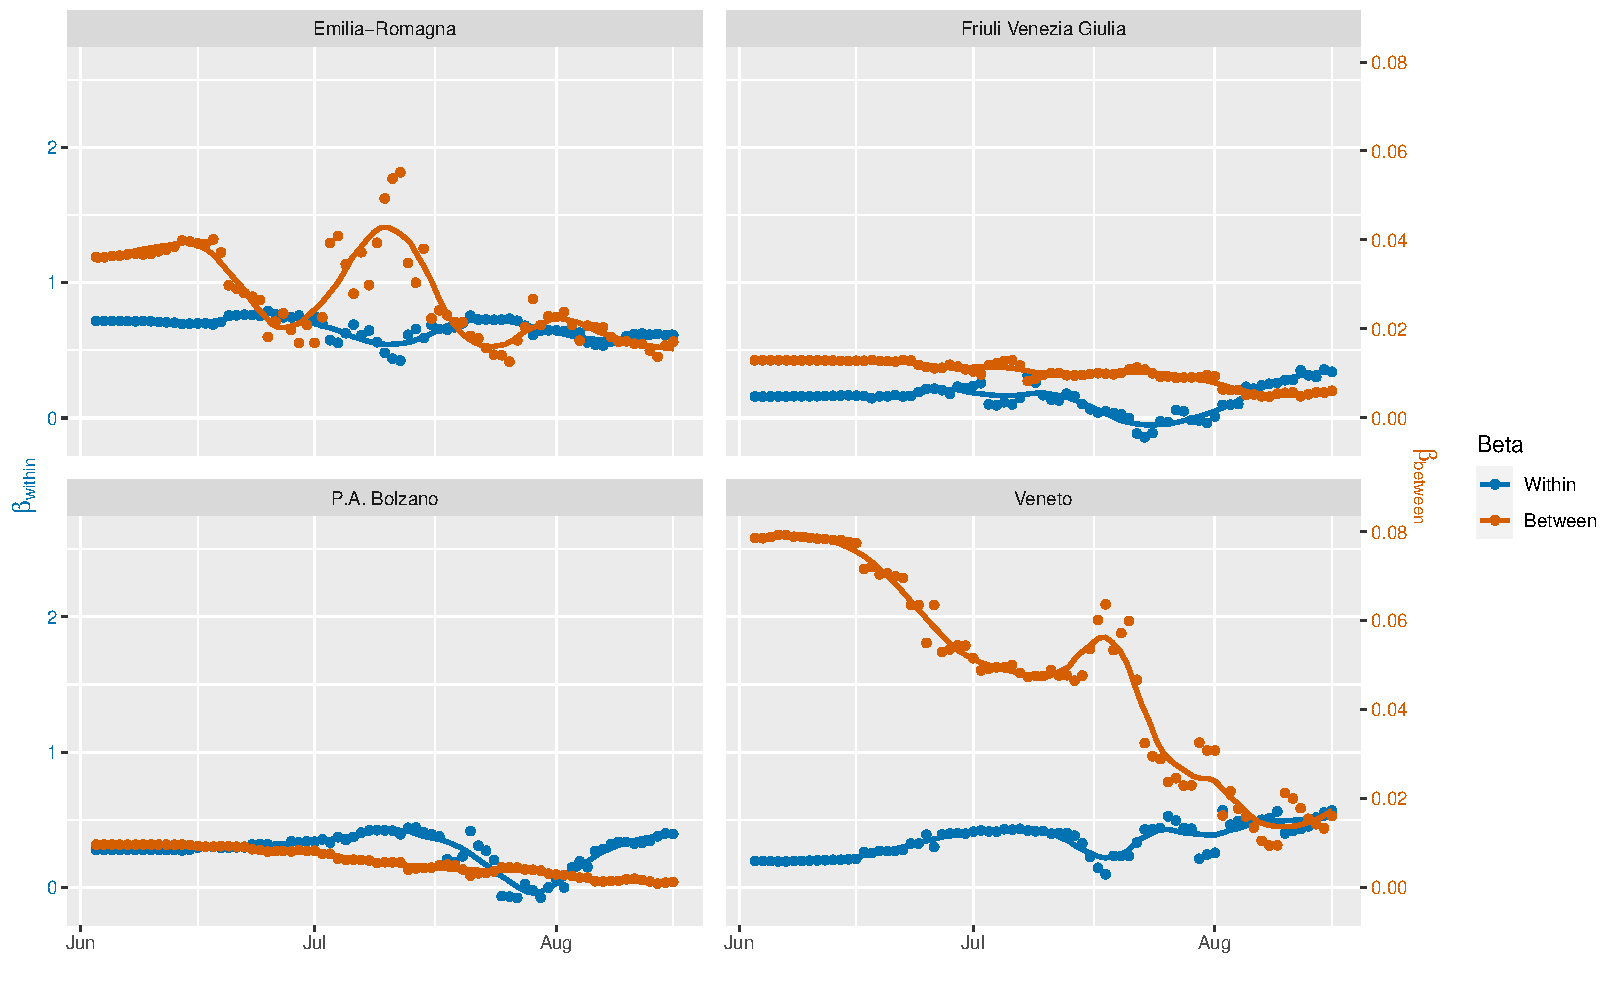
\includegraphics[width=0.95\linewidth]{output/model3_lag3_betas_Nord-Est_rolling.pdf}
	      \caption{Without model selection}
	      \label{fig:beta_within_between_over_time_nordest_regular}
	    \end{subfigure}\newline
	    \begin{subfigure}{\textwidth}
	      \centering
	      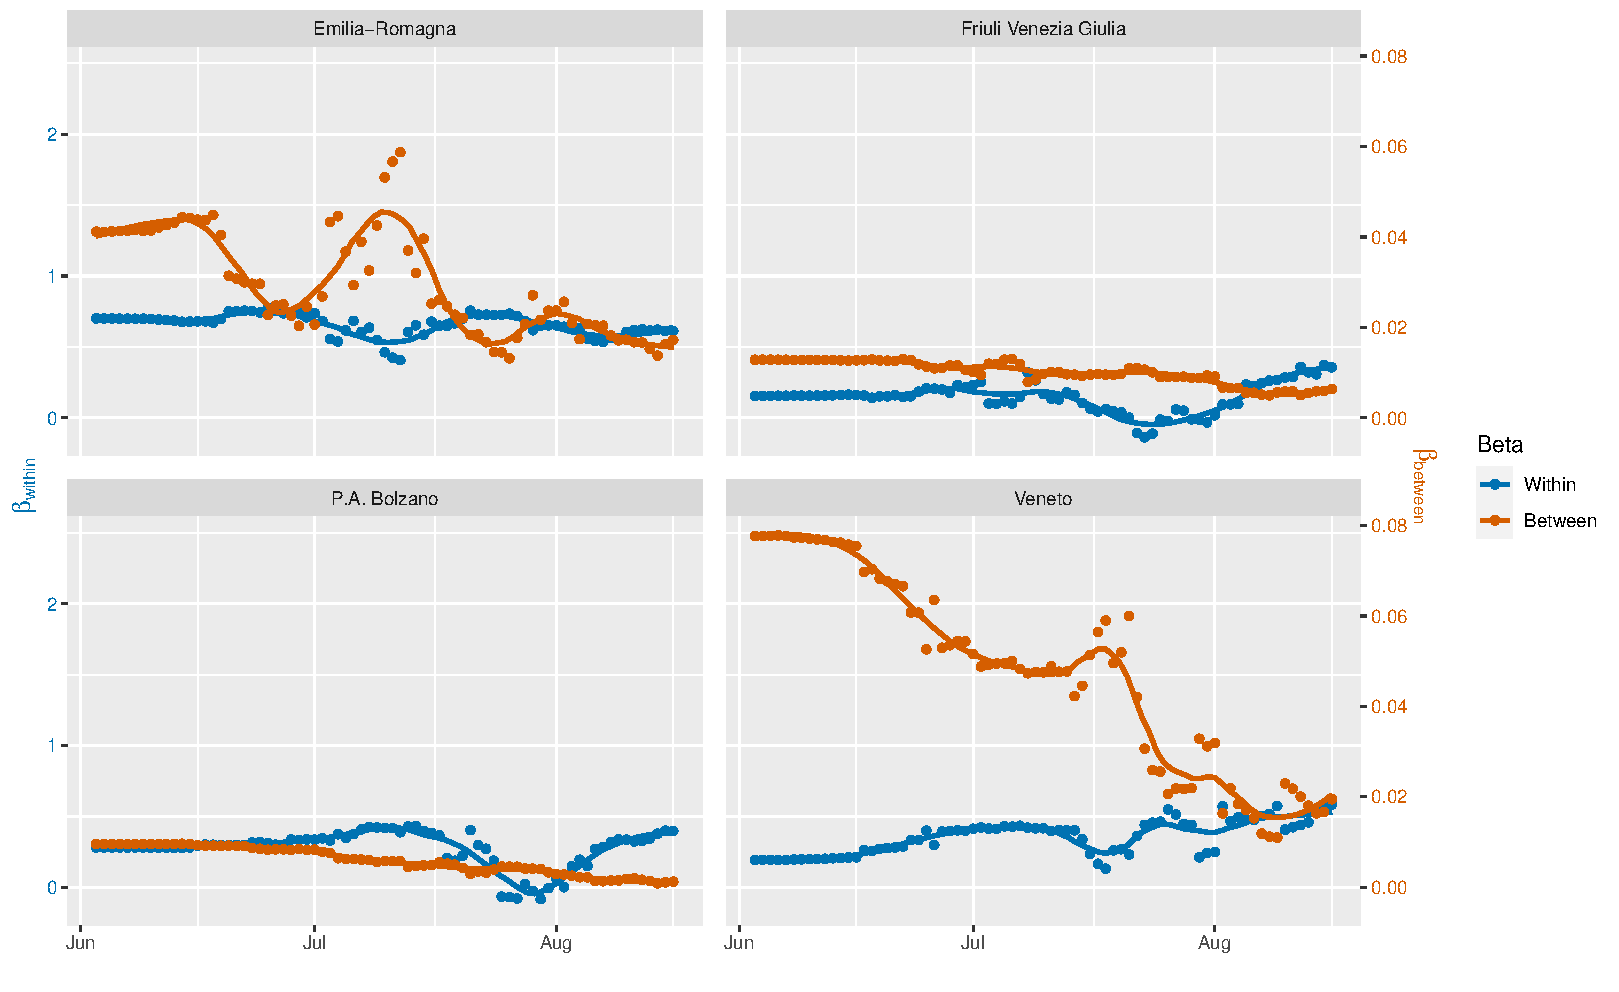
\includegraphics[width=0.95\linewidth]{output/model3_lag3_betas_Nord-Est_aic_rolling.pdf}
	      \caption{With model selection by AIC}
	      \label{fig:beta_within_between_over_time_nordest_aic}
	    \end{subfigure}
	\end{figure}
    \begin{figure}[H]\ContinuedFloat
	    \begin{subfigure}{\textwidth}
	      \centering
	      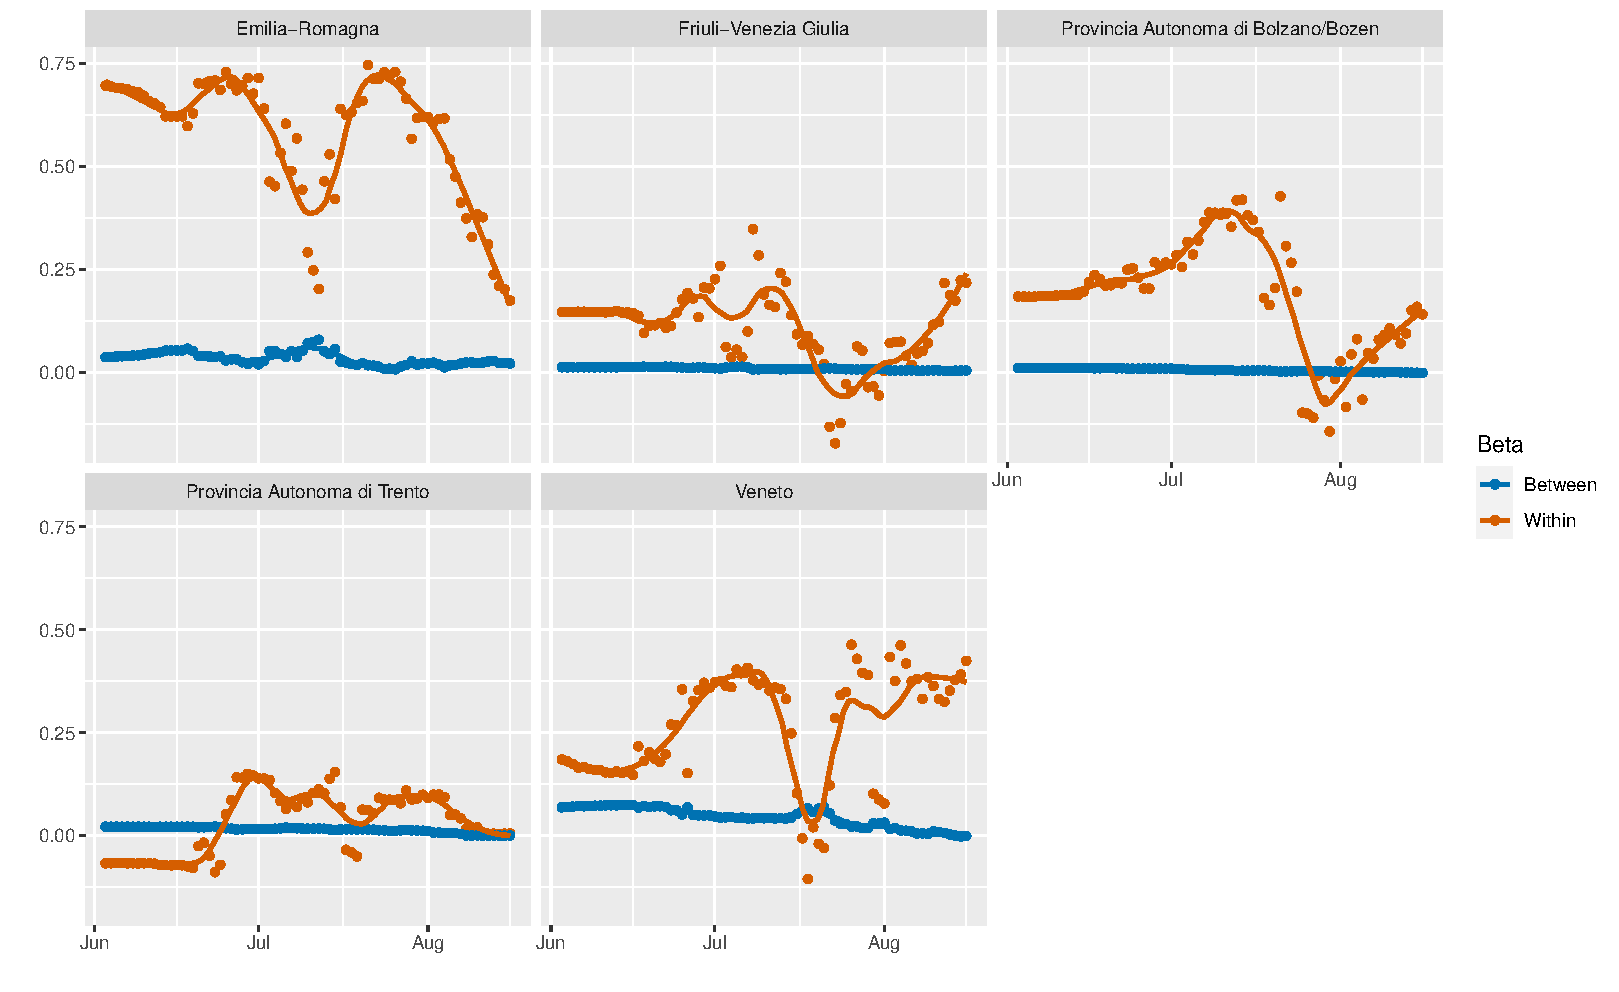
\includegraphics[width=0.95\linewidth]{output/model3_lag3_betas_Nord-Est_UndocQuadratic_rolling.pdf}
	      \caption{Without model selection; \\ including undocumented infectives}
	      \label{fig:beta_within_between_over_time_nordest_regular_undoc}
	    \end{subfigure}\newline
	    \begin{subfigure}{\textwidth}
	      \centering
	      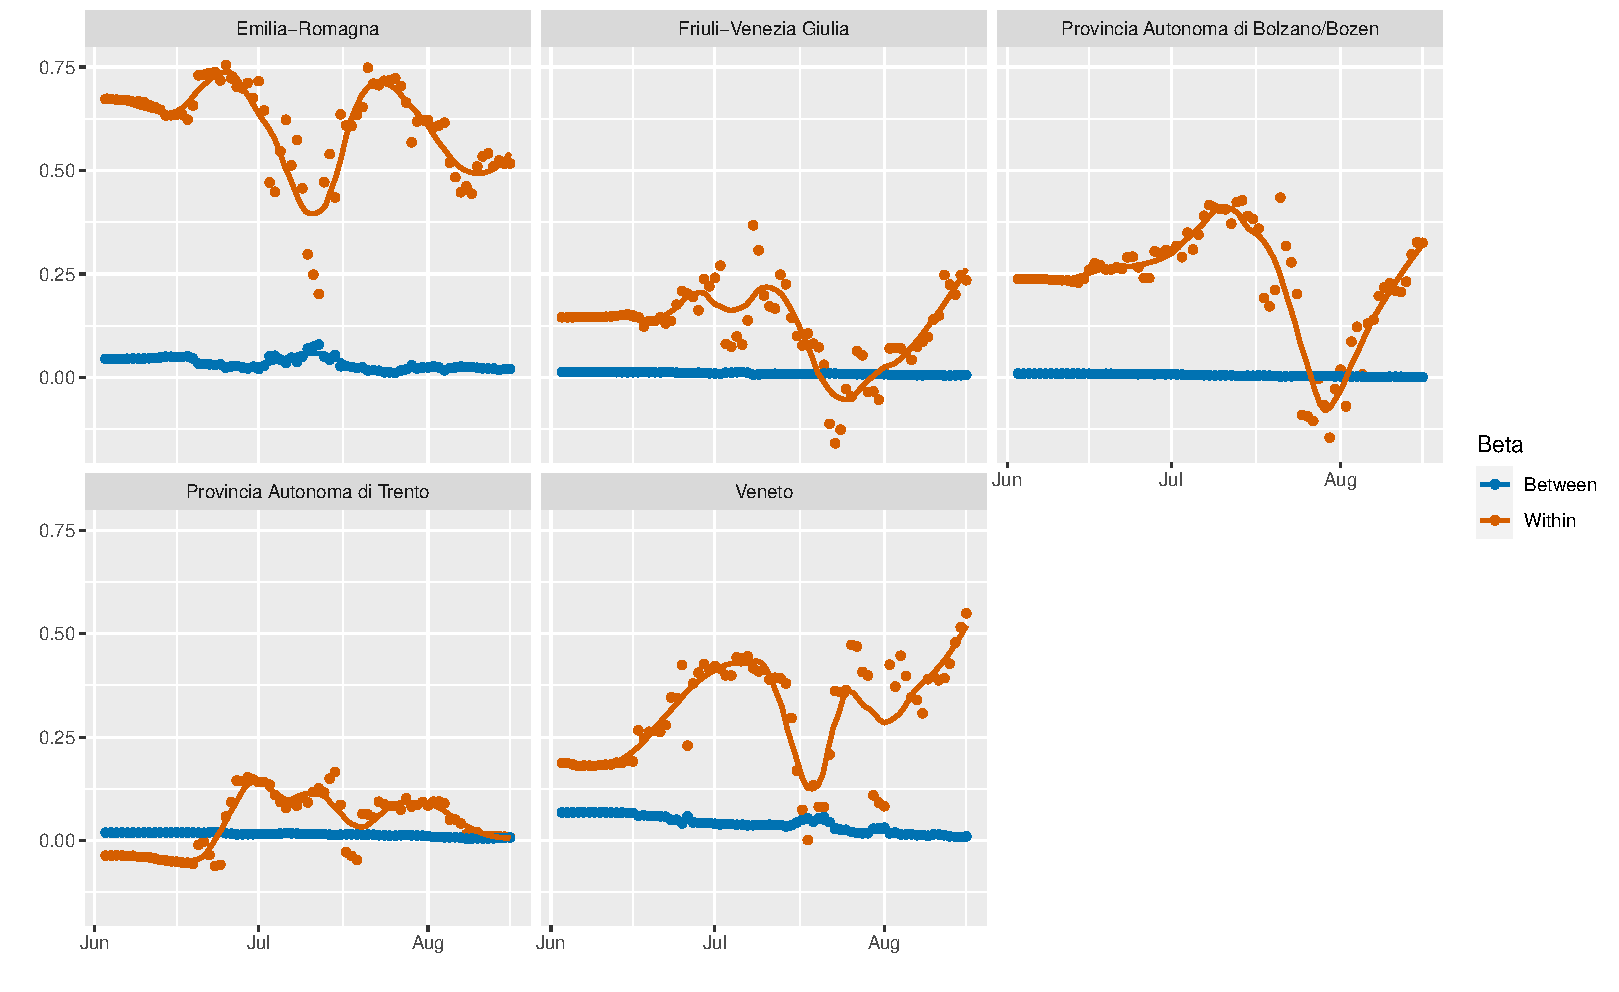
\includegraphics[width=0.95\linewidth]{output/model3_lag3_betas_Nord-Est_aic_UndocQuadratic_rolling.pdf}
	      \caption{With model selection by AIC; \\ including undocumented infectives}
	      \label{fig:beta_within_between_over_time_nordest_aic_undoc}
	    \end{subfigure}
	    \caption{Progression of $\beta_{within}$ and $\beta_{between}$ over time for the \textit{Nord-Est} (North-East) NUTS 1 region}
	    \label{fig:beta_within_between_over_time_nordest}
    \end{figure}
	
	Figure \ref{fig:beta_within_between_over_time_nordest} shows very different patterns compared to the within-region spread model, as discussed in the previous section. Firstly, we do not see a decreasing movement for $\beta_{within}$. In contrast, the values seem to fluctuate around some value. For $\beta_{between}$, we also see some fluctuation but we do generally see a decreasing movement. For the other NUTS 1 regions, we see some similar patterns although the progression varies a lot over the regions. For instance, the estimate for $\beta_{between}$ for the region of Lazio tends to increase over time, as can be seen in Figure \ref{fig:beta_within_between_over_time_centro}. Model selection by AIC does not seem to impact the estimates of $\beta_{within}$ and $\beta_{between}$ much.
	
	\section{Model selection} \label{sec:model_selection}
	One can imagine that the same model specification does not apply to all Italian regions. For this reason, we apply model selection on the regressors included in the tensor $M$. For model selection, we use the Akaike Information Criterion or AIC \parencite{akaike1974new}. The AIC for a particular model is defined as
	\begin{equation} \label{eq:AIC}
    	AIC = -2\log(ML) + 2k,    
	\end{equation}
	where $ML$ denotes the maximum likelihood for the model and $k$ denotes the number of parameters in the model. In contrast, one could also consider the Bayesian Information Criterion or BIC \parencite{schwarz1978estimating}. \textcite{schwarz1978estimating} developed it as an alternative to the Akaike Information Criterion. The BIC is defined as
	\begin{equation} \label{eq:BIC}
    	BIC = -2\log(ML) + k\log(n),
	\end{equation}
	where $n$ denotes the sample size. Both the AIC and BIC are used as the minimizer in the model selection. That is, the model that is picked by the model selection procedure is the one with the lowest AIC or BIC. When choosing between the two methods, one should realize that they have different properties, particularly related to consistency. The AIC tends to select a larger model than the BIC. Moreover, if the true model is included in the set of candidate models, and under some additional assumptions, the BIC will select the true model with probability one as $n$ goes to infinity whereas the AIC is not consistent. On the other hand, if the true model is not in the set of candidate models, clearly no method can possibly select the true model. However, the AIC is efficient in the sense that it will asymptotically select the model that minimizes the mean prediction error while the BIC is not efficient \parencite{vrieze2012model}. Proponents of using the AIC over the BIC argue that this shows that the AIC is to be preferred because it is virtually impossible for the true model to be constructed because \textit{``all models are wrong"} \parencite{box1976science}. That does not mean that reality cannot be modelled; some models can be useful despite not being perfectly true. \textcite{burnham2002practical} state that \textit{``A model is a simplification or approximation of reality and hence will not reflect all of reality. [...] While a model can never be ``truth," a model might be ranked from very useful, to useful, to somewhat useful to, finally, essentially useless".} Lastly, \textcite{vrieze2012model} shows by simulation that the BIC can fail in finite sample sizes even if the true model is in the candidate set. This is because the BIC has a higher maximum risk, defined as the mean squared error of estimating the true covariance matrix. Because we believe that, indeed, the true model generating the data will quite likely not be included in our candidate set, we use the AIC to perform model selection.
	
	\section{Discrete SIR Model}\label{sec:discrete_sir_model}
	As explained in Section \ref{sec:model_within}, there are several steps made by \textcite{adda2016economic} that are not explained clearly in the paper and that do not seem to mathematically grounded. In this section, we provide our own derivation for a discrete SIR model. We start by explaining the two versions of the SIR model, as eluded to in Section \ref{sec:sir_model}, after which we will describe our own discrete SIR model. Lastly, we will discuss the two methods that are being used to estimate the parameters, in addition to the regional split, in Sections \ref{subsec:discrete_sir_panel} and \ref{subsec:discrete_sir_bayesian}. \\
	
	As mentioned in Section \ref{sec:sir_model}, there are two versions of the SIR model, namely with frequency-dependent and with density-dependent transmission. For the former, the proportion of people in each of the groups is used ($S$, $I$, and $R$) while in the latter, the absolute number of people is used ($s$, $i$, and $r$). \textcite{keeling2011modeling} explain that the distinction in applicability is based on the assumption that we make on the relationship between the contact rate and the population size. For frequency-dependent transmission, also called random mixing, these are assumed to be independent whereas for density-dependent transmission it is assumed that the contact rate increases with the population density. Therefore, \textcite{keeling2011modeling} state that frequency-dependent transmission is generally applied when considering a heterogeneous contact structure, which means that everyone interacts with one another with equal probability. Density-dependent transmission is, on the other hand, generally applied to plant and animal diseases. \\
	
	To illustrate the logic behind this, consider an infection that is transmitted sexually. \textcite{keeling2011modeling} give an example for chlamydia in a koala population. When considering a human population, frequency-dependent transmission is often used because a higher density of people does not seem to imply a higher sexual activity, i.e. the sexual contact structure is heterogenous. For some animals, however, a higher density may imply that more sexual activity occurs and, therefore, density-dependent transmission may be more applicable. \\
	
	Now, let us consider the coronavirus SARS-CoV-2. Firstly, notice that we consider a human population so, therefore, frequency-dependent transmission may be more applicable. However, it is also intuitive that the transmission of SARS-CoV-2 is higher at the moment that more people live in a certain area because, at that point, people can be expected to come into contact with one another more. However, policies that are employed by governments may guarantee a less density-dependent situation, for instance, when governments instate a lockdown, oblige the use of face masks, or promote social distancing. Around 70\% of the papers assume no relationship between density and transmission. In the other 30\% of the cases, a linear relationship is assumed \parencite{nightingale2020importance}. The issue with this, according to \textcite{nightingale2020importance}, is that, respectively, there is an underestimation or overestimation of the delay in infection resurgence after mass quarantining ends. Because we are not interested in estimating the infection resurgence, we expect these issues to not be apparent, although we recognize that a transmission structure that lies somewhere in between would be ideal. \\
	
	In this thesis, we look at both versions of the SIR model and compare the results in Section \ref{subsec:results_discrete_sir}. The derivations that are done in this section are for the frequency-dependent version of the SIR model. Of course, we can simply replace the variables $S$, $I$, and $R$ by $s$, $i$, and $r$, respectively, to obtain the formulations for the models using density-dependent transmission. \\
	
	Recall from \eqref{eq:SIR_model_S}-\eqref{eq:SIR_model_R} that the SIR model with frequency-dependent transmission is given by:
	    \begin{align*}
    	    \frac{dS}{dt} &= -\beta SI + \omega R, \\
    	    \frac{dI}{dt} &= \beta SI - \gamma I, \\
    	    \frac{dR}{dt} &= \gamma I - \omega R.
	    \end{align*}
	
	In Section \ref{sec:sir_model} we discussed that the parameter $\omega$ represents the immunity. We explained that it is currently unclear whether people develop some sort of immunity to COVID-19. However, we did state that this immunity likely lasts long enough throughout our sample since we do not consider an analysis over multiple years. Therefore, under the assumption that $\omega = 0$, these equations simplify to the following:
	    \begin{align}
    	    \frac{dS}{dt} &= -\beta SI, \label{eq:SIR_model_S_simplified} \\
    	    \frac{dI}{dt} &= \beta SI - \gamma I, \label{eq:SIR_model_I_simplified} \\
    	    \frac{dR}{dt} &= \gamma I. \label{eq:SIR_model_R_simplified}
	    \end{align}
    	
	When taking the possible estimation error $\eta_{r,t}$, whether from discretizing or estimating the parameters, into account, these equations are equivalent to:
	    \begin{align}
        	S_{r,t} - S_{r,t-1} &= -\beta S_{r,t-1}I_{r,t-1} + \eta_{r,t}, \label{eq:SIR_model_S_discrete}\\
        	I_{r,t} - I_{r,t-1} &= \beta S_{r,t-1}I_{r,t-1} - \gamma I_{r,t-1} + \eta_{r,t}, \label{eq:SIR_model_I_discrete}\\
        	R_{r,t} - R_{r,t-1} &= \gamma I_{r,t-1} + \eta_{r,t}. \label{eq:SIR_model_R_discrete}
    	\end{align}
	
	As such, if the data available on $S$, $I$, and $R$ are indeed deemed to be accurate, then $\beta$ and $\gamma$ are readily estimated from \ref{eq:SIR_model_S_discrete} and \ref{eq:SIR_model_R_discrete}. The results from estimating the parameters in this way are presented in Section \ref{subsec:results_discrete_sir}. \\
	
	Because we are interested in the number of infectives, we will consider equation \eqref{eq:SIR_model_I_discrete}. The right-hand side of this equation consists of three terms. Firstly, the term $\beta S_{r,t-1}I_{r,t-1}$ relates to the observation that new infectives are formed due to interaction of infectives with the susceptible population, i.e. the people that move from the group $s$ to the group $i$. In Section \ref{sec:sir_model}, we explained that it is assumed that this rate $\beta$ is constant over time. However, we concede that the addition of introducing a longer lag that \textcite{adda2016economic} makes is valid. Indeed, when a susceptible person meets an infective and consequently gets infected, this person is not immediately infectious themselves. For the same reasons as laid out in Section \ref{sec:model_within}, we can replace the lag in the first term by a longer lag $\tau$, which we would set to be equal to the estimated latent period of three days. The following model would then be the result:
	    \begin{equation}\label{eq:SIR_model_I_discrete_tau}
            I_{r,t} - I_{r,t-1} = \beta S_{r,t-\tau}I_{r,t-\tau} - \gamma I_{r,t-1} + \eta_{r,t}
        \end{equation}
	
	Similarly, we transform equation \eqref{eq:SIR_model_S_discrete} in the same way:
	    \begin{equation}\label{eq:SIR_model_S_discrete_tau}
            S_{r,t} - S_{r,t-1} = -\beta S_{r,t-\tau}I_{r,t-\tau} + \eta_{r,t}
        \end{equation}
	
	We will report results with $\tau=1$ and $\tau=3$ in Section \ref{subsec:results_discrete_sir}. The second term in \eqref{eq:SIR_model_I_discrete} is $-\gamma I_{r,t-1}$, which describes the infectives that recover or die from the disease, i.e. the people that move from group $i$ to group $r$. Note that we have not included the lag $\tau$ in this term. This is because when a person recovers from the disease they immediately move to that group. This also applies to the same term in equation \eqref{eq:SIR_model_R_discrete}. Lastly, as mentioned in the previous paragraph, $\eta_{r,t}$ denotes the idiosyncratic error term. \\
	
	As mentioned earlier in this section, if one believes the data on all components to be correct, these parameters can be easily identified. However, note that $S_{r,t-\tau}$ is generally quite close to 1: most of the population is susceptible to contracting the virus. That means that it is difficult to identify the parameters jointly. Suppose that $S_{r,t-\tau}$ is indeed equal to 1, for simplification purposes. Then, the right-hand side of \eqref{eq:SIR_model_I_discrete_tau} becomes $\beta I_{r,t-\tau} - \gamma I_{r,t-1}$. It is probable that $I_{r,t-\tau}$ and $I_{r,t-1}$ are quite close to one another, meaning that they cannot be jointly identified by means of equation \eqref{eq:SIR_model_I_discrete_tau}. As such, we need to employ a two-step approach. \\
	
	We propose two methods. Firstly, we can apply estimation methods to \eqref{eq:SIR_model_S_discrete_tau} and \eqref{eq:SIR_model_R_discrete} individually to obtain the estimates for $\beta$ and $\gamma$ individually. The second method would be to first estimate one of the parameters by means of \eqref{eq:SIR_model_R_discrete} \eqref{eq:SIR_model_S_discrete_tau}. Secondly, we would fill in this estimate in \eqref{eq:SIR_model_I_discrete_tau} and estimate the remaining parameter. We use equation \ref{eq:SIR_model_R_discrete} to estimate $\gamma$ and use the resulting estimate $\hat{\gamma}$ in \eqref{eq:SIR_model_I_discrete_tau} to obtain:
	    \begin{align*}
	        & I_{r,t} - I_{r,t-1} = \beta S_{r,t-\tau}I_{r,t-\tau} - \hat{\gamma} I_{r,t-1} + \eta_{r,t} \\
	        \iff & I_{r,t} - \left(1 - \hat{\gamma}\right) I_{r,t-1} = \beta S_{r,t-\tau}I_{r,t-\tau} + \eta_{r,t} \numberthis{\label{eq:SIR_model_I_discrete_twostep}}
	    \end{align*}
	
	Another solution, if one does not believe in the accuracy of the data, is to write the difference in the number of removed individuals as a function of the constant rate $\gamma$ and the infectives. This is then included in the calculation of the susceptible population by means of a function, after which nonlinear least-squares (NLS) can be applied. \todo[inline, backgroundcolor=green!40]{TODO: Continue here: NLS}
	
	\subsection{Panel data methods}\label{subsec:discrete_sir_panel}
	The discrete SIR equations in \eqref{eq:SIR_model_R_discrete}, \eqref{eq:SIR_model_S_discrete_tau}, and \eqref{eq:SIR_model_I_discrete_twostep} are estimated by panel data methods and Bayesian estimation. We first discuss the panel data methods. Panel data refers to a dataset that contains measurements over time for a group of individuals. In our case, the individuals are represented by the $R$ regions and we have observations for $T$ time periods. The main motivation behind using panel data methods is that they comprise more information, making them more efficient. Moreover, because the same individual is observed multiple times over time, they are able to identify unobserved individual effects (heterogeneity) that are persistent over time, such as an aversion to spending money or another effect that causes an individual that experienced some event in the past to experience that effect in the future again with a higher probability. A regular cross-sectional model is usually described as:
	    \begin{equation}\label{eq:cross-section}
    	    y_i = x_i'\theta + \epsilon_i, \quad\forall i=1,\dotsc,R
	    \end{equation}
	where $y$ denotes the dependent variable, $x$ denotes the independent variables, $\theta$ is the vector of parameters to be estimated, and $\epsilon$ is an idiosyncratic error term. A panel data model is usually described in a very similar way:
	    \begin{equation}\label{eq:paneldata}
	        y_{i,t} = x_{i,t}'\theta + \epsilon_{i,t}, \quad\forall i=1,\dotsc,R;~t=1,\dotsc,T
	    \end{equation}
	where the error component $\epsilon_{i,t} \coloneqq \alpha_i + u_{i,t}$ is a composite error term, comprising a time-invariant individual effect, denoted by $\alpha_i$, and an idiosyncratic error term, denoted by $u_{i,t} \sim N\left(0, \sigma^2_u\right)$. We assume that the individual effect is not correlated with the regressors:
	    \begin{equation}\label{eq:orthogonality_assumption}
	        E\left[\alpha_i \,\middle|\, x_{i,1}, \dotsc, x_{i, T}\right] = 0
	    \end{equation}
	    
	As an example, for equation \eqref{eq:SIR_model_I_discrete_twostep}, note that:
	    \begin{equation*}
	        y_{i,t} = I_{r,t} - \left(1 - \hat{\gamma}\right) I_{r,t-1}, \quad
	        \theta = \beta, \quad
            x_{i,t} = S_{r,t-\tau}I_{r,t-\tau}, \quad
            u_{i,t} = \eta_{r,t}
	    \end{equation*}
	    
	Looking at this notation, we can see that it is safe to impose the assumption that the individual effect and the independent variables are orthogonal: it seems odd to assume that the individual regional effect, which is time-invariant, is correlated with the time-varying incidence rate or susceptible rate of this one specific disease. In the rest of this section, we will follow the notation as in \eqref{eq:paneldata} but one can follow the example to formulate these in terms of the SIR equations. \\
	
	There are three main panel data models that are usually applied: the pooled OLS (POLS), fixed effects (FE), and random effects (RE) models. The choice between these models depends on the assumptions that are placed on the individual effect $\alpha_i$. For each of these three methods, we define them and discuss the required exogeneity assumption(s) and possible other interesting features. We will start with the fixed effects model because the way it is defined is inconsistent with the epidemiological literature on the SIR model. Next, we will consider the random effects model, after which we discuss the pooled OLS model. \\
	
	The fixed effects model makes no assumptions about the time-invariant individual effect but applies a within-transformation, namely time-demeaning the data, to eliminate it from the model. The effect is that all time-invariant regressors, such as dummy variables gender or one's education level, are also eliminated from the model. The fixed effects model is then to apply OLS to the time-demeaned data to obtain the estimates of $\theta$. The model mentions fixed effects in its name because, in essence, it assumes that each individual (region) has a time-constant intercept. This is assumed to be different from zero; otherwise, we could apply the pooled OLS model described at the end of this section. The SIR model, on the other hand, does not include an intercept in its formulation. The reason behind this is intuitive: there is not some non-zero mean number of new cases that is persistent throughout time for a certain region. Because of this, the fixed effects model is not suitable for our estimation. \\
	
	The main idea behind the random effects model is to impose a distribution on the individual effects that can then be included in the error term. The random effects model equation is identical to \eqref{eq:paneldata}, where we assume that $\alpha_i \sim N\left(0, \sigma^2_{\alpha}\right)$. Note that this assumption may be in line with the SIR model because the mean heterogeneous effect is assumed to be zero. Because the individual effect is now included in the error term, we need to impose assumptions on the entire composite error term. Firstly, the random effects model requires the strict exogeneity assumption:
	    \begin{equation}\label{eq:strict_exogeneity}
	        E\left[u_{i,t} \,\middle|\, \alpha_i, x_{i,1}, \dotsc, x_{i, T}\right] = 0, \quad\forall t=1,\dotsc,T 
	    \end{equation}
	    
	This assumption essentially says that the variables are not allowed to depend on any of the errors, whether in the past, present, or future. However, because the individual effects are included in the error term, we need strict exogeneity between $\epsilon_{i,t}$ and $x_{i,t}$ as well. This is achieved by the assumption that the individual effect is not correlated with the regressors in \eqref{eq:orthogonality_assumption}. As such, combining the strict exogeneity assumption and the orthogonality assumption, the aforementioned strict exogeneity assumption between $\epsilon_{i,t}$ and $x_{i,t}$ holds. We will not delve into the details of how the random effects model is specifically estimated; suffice to say that it is estimated by generalized least squares (GLS). \\
	
	Lastly, we discuss pooled OLS. This model ignores the individual effect, hence treating the data as one large cross-section. This means that the $T$ observations for some individual $i$ are actually treated to be cross-sectional observations of $T$ different individuals. The exogeneity assumption that needs to be satisfied is a simple exogeneity assumption:
	    \[E(x_{i,t}\epsilon_{i,t}) = 0 \text{, so } E(x_{i,t}u_{i,t}) = 0 \text{ and } E(x_{i,t}\alpha_i) = 0\]
	
	Because we expect that there will be a vast difference between the Italian regions, as eluded to in Section \ref{sec:problem_description}, pooled OLS is likely not a good model for this thesis. Nonetheless, we estimate the results and compare them to those of the random effects model.
	
	\subsection{Bayesian estimation methods}\label{subsec:discrete_sir_bayesian}
	In the last few months, a lot of research has been done on the spread of SARS-CoV-2 for various locales. Therefore, we may have some idea of what the values of the parameters are likely to be.
	\todo[inline, backgroundcolor=green!40]{TODO: Continue here}
	
	\subsection{Results}\label{subsec:results_discrete_sir}
	\todo[inline, backgroundcolor=green!40]{TODO: Results still need to be inserted}
	
	In this section, we present the results for the discrete SIR model presented in Section \ref{sec:discrete_sir_model}. Recall that we mentioned three estimation approaches, namely the regular regional splits as applied for the models by \textcite{adda2016economic}, panel data methods, and Bayesian analysis. We will present the results in said order. For all result tables, we again apply a rolling window as before and report the results for two values of the lag parameter $\tau$, namely 1 and 3, as explained in Section \ref{sec:discrete_sir_model}. \\
	
	When applying the methodology as explained in Section \ref{sec:discrete_sir_model} to the regional models, there is no panel data structure anymore. Therefore, the results presented in Tables X\todo[backgroundcolor=green!40]{TODO: Table} are estimated with OLS. First off, we present the results comparing frequency-dependent transmission and density-dependent transmission in Table \ref{tab:results_discrete_regional_transmission}.
	
	\begin{landscape}
	\begin{longtable}{@{}lccccccc@{}}
	    \caption{Estimates for the discrete SIR model per region comparing frequency-dependent and density-dependent transmission. Estimates are given with $t$-statistics in parentheses. Data spans May 9 till August 16, 2020 (100 days). Undocumented infectives are not modelled. A lag of $\tau=1$ is used.}
		\label{tab:results_discrete_regional_transmission}\\
		\toprule
		                & \multicolumn{3}{c}{Frequency-dependence} & \multicolumn{3}{c}{Density-dependence} \\
		                \cmidrule(lr){2-4}
                        \cmidrule(lr){5-7}
		Region          & $\beta$ & $\beta_{two-step}$ & $\gamma$ & $\beta$ & $\beta_{two-step}$ & $\gamma$ \\* \midrule
		\endfirsthead
		
		\multicolumn{7}{c}{{\bfseries Table \thetable\ continued from previous page}} \\
		\toprule
		                & \multicolumn{3}{c}{Frequency-dependence} & \multicolumn{3}{c}{Density-dependence} \\
		                \cmidrule(lr){2-4}
                        \cmidrule(lr){5-7}
		Region          & $\beta$ & $\beta_{two-step}$ & $\gamma$ & $\beta$ & $\beta_{two-step}$ & $\gamma$ \\* \midrule
		\endhead
		
		\bottomrule
		\multicolumn{7}{c}{{\bfseries Table \thetable\ continues on next page}}
		\endfoot
		
		\multicolumn{7}{c}{Significance levels: * = 0.1 ** = 0.05, *** = 0.01}
		\endlastfoot
        National & $4.976 \times 10^{-5}$*** & 0.011*** & $3.626 \times 10^{-5}$*** & $1.052 \times 10^{-12}$*** & $2.289 \times 10^{-10}$*** & $3.62516 \times 10^{-5}$*** \\ 
        National\_zvals & (6.544) & (31.512) & (5.571) & (6.485) & (31.517) & (5.571) \\ 
        ABR & $6.890 \times 10^{-3}$*** & $7.247 \times 10^{-3}$*** & $5.749 \times 10^{-3}$*** & $5.536 \times 10^{-9}$*** & $5.534 \times 10^{-9}$*** & $5.749 \times 10^{-3}$*** \\ 
        ABR\_zvals & (8.637) & (38.656) & (7.216) & (8.747) & (38.649) & (7.216) \\ 
        BAS & $6.917 \times 10^{-3}$*** & $6.962 \times 10^{-3}$*** & $4.418 \times 10^{-3}$*** & $1.239 \times 10^{-8}$*** & $1.239 \times 10^{-8}$*** & $4.418 \times 10^{-3}$*** \\ 
        BAS\_zvals & (5.234) & (6.904) & (5.221) & (5.260) & (6.904) & (5.221) \\ 
        BZ & $3.248 \times 10^{-3}$*** & $3.258 \times 10^{-3}$*** & $2.297 \times 10^{-3}$*** & $6.148 \times 10^{-9}$*** & $6.146 \times 10^{-9}$*** & $2.297 \times 10^{-3}$*** \\ 
        BZ\_zvals & (9.265) & (29.559) & (7.005) & (9.263) & (29.559) & (7.005) \\ 
        CAL & $7.467 \times 10^{-3}$*** & $7.522 \times 10^{-3}$*** & $5.609 \times 10^{-3}$*** & $3.869 \times 10^{-9}$*** & $3.869 \times 10^{-9}$*** & $5.609 \times 10^{-3}$*** \\ 
        CAL\_zvals & (8.048) & (22.664) & (6.148) & (8.022) & (22.664) & (6.148) \\ 
        EMR & $4.501 \times 10^{-3}$*** & $4.730 \times 10^{-3}$*** & $3.329 \times 10^{-3}$*** & $1.063 \times 10^{-9}$*** & $1.063 \times 10^{-9}$*** & $3.328 \times 10^{-3}$*** \\ 
        EMR\_zvals & (11.873) & (67.727) & (9.116) & (11.811) & (67.807) & (9.116) \\ 
        FVG & $4.339 \times 10^{-3}$*** & $4.457 \times 10^{-3}$*** & $3.255 \times 10^{-3}$*** & $3.675 \times 10^{-9}$*** & $3.674 \times 10^{-9}$*** & $3.255 \times 10^{-3}$*** \\ 
        FVG\_zvals & (7.690) & (39.723) & (6.287) & (7.744) & (39.722) & (6.287) \\ 
        LAZ & $8.194 \times 10^{-3}$*** & $8.570 \times 10^{-3}$*** & $6.036 \times 10^{-3}$*** & $1.460 \times 10^{-9}$*** & $1.460 \times 10^{-9}$*** & $6.036 \times 10^{-3}$*** \\ 
        LAZ\_zvals & (6.581) & (53.328) & (4.813) & (6.666) & (53.330) & (4.813) \\ 
        LIG & $5.978 \times 10^{-3}$*** & $6.271 \times 10^{-3}$*** & $4.487 \times 10^{-3}$*** & $4.056 \times 10^{-9}$*** & $4.053 \times 10^{-9}$*** & $4.486 \times 10^{-3}$*** \\ 
        LIG\_zvals & (7.476) & (33.236) & (6.626) & (7.553) & (33.253) & (6.626) \\ 
        LOM & $6.210 \times 10^{-3}$*** & $6.415 \times 10^{-3}$*** & $4.565 \times 10^{-3}$*** & $6.399 \times 10^{-10}$*** & $6.394 \times 10^{-10}$*** & $4.564 \times 10^{-3}$*** \\ 
        LOM\_zvals & (10.809) & (37.672) & (9.531) & (10.786) & (37.699) & (9.530) \\ 
        MAR & $6.097 \times 10^{-3}$*** & $6.141 \times 10^{-3}$*** & $5.263 \times 10^{-3}$*** & $4.037 \times 10^{-9}$*** & $4.035 \times 10^{-9}$*** & $5.263 \times 10^{-3}$*** \\ 
        MAR\_zvals & (7.691) & (53.351) & (6.883) & (7.686) & (53.366) & (6.883) \\ 
        MOL & 0.010*** & 0.010*** & $6.753 \times 10^{-3}$*** & $3.293 \times 10^{-8}$*** & $6.753 \times 10^{-3}$*** \\ 
        MOL\_zvals & (6.835) & (11.366) & (6.638) & (6.855) & (11.366) & (6.638) \\ 
        PIE & $6.309 \times 10^{-3}$*** & $6.566 \times 10^{-3}$*** & $5.313 \times 10^{-3}$*** & $1.512 \times 10^{-9}$*** & $1.510 \times 10^{-9}$*** & $5.312 \times 10^{-3}$*** \\ 
        PIE\_zvals & (8.138) & (48.683) & (7.794) & (8.129) & (48.752) & (7.794) \\ 
        PUG & $7.622 \times 10^{-3}$*** & $7.862 \times 10^{-3}$*** & $6.513 \times 10^{-3}$*** & $1.955 \times 10^{-9}$*** & $1.954 \times 10^{-9}$*** & $6.513 \times 10^{-3}$*** \\ 
        PUG\_zvals & (8.617) & (47.630) & (7.346) & (8.655) & (47.629) & (7.346) \\ 
        SAR & $5.487 \times 10^{-3}$*** & $5.594 \times 10^{-3}$*** & $5.374 \times 10^{-3}$*** & $3.418 \times 10^{-9}$*** & $3.417 \times 10^{-9}$*** & $4.374 \times 10^{-3}$*** \\ 
        SAR\_zvals & (6.843) & (24.746) & (5.531) & (6.884) & (24.745) & (5.531) \\ 
        TOS & $5.704 \times 10^{-3}$*** & $5.902 \times 10^{-3}$*** & $4.785 \times 10^{-3}$*** & $1.586 \times 10^{-9}$*** & $1.585 \times 10^{-9}$*** & $4.785 \times 10^{-3}$*** \\ 
        TOS\_zvals & (7.043) & (57.604) & (6.124) & (7.157) & (57.601) & (6.124) \\ 
        UMB & $2.160 \times 10^{-3}$*** & $2.222 \times 10^{-3}$*** & $1.217 \times 10^{-3}$*** & $2.523 \times 10^{-9}$*** & $2.523 \times 10^{-9}$*** & $1.217 \times 10^{-3}$*** \\ 
        UMB\_zvals & (8.453) & (13.646) & (6.331) & (8.602) & (13.645) & (6.331) \\ 
        VDA & $2.017 \times 10^{-3}$*** & $2.076 \times 10^{-3}$*** & $1.489 \times 10^{-3}$*** & $1.656 \times 10^{-8}$*** & $1.655 \times 10^{-8}$*** & $1.488 \times 10^{-3}$*** \\ 
        VDA\_zvals & (6.145) & (16.797) & (5.591) & (6.186) & (16.796) & (5.590) \\ 
        VEN & $4.781 \times 10^{-3}$*** & $5.018 \times 10^{-3}$*** & $3.619 \times 10^{-3}$*** & $1.025 \times 10^{-9}$*** & $1.025 \times 10^{-9}$*** & $3.619 \times 10^{-3}$*** \\ 
        VEN\_zvals & (9.239) & (31.058) & (7.151) & (9.273) & (31.047) & (7.151) \\* \bottomrule
	\end{longtable}
	\end{landscape}
	
	Table \ref{tab:results_discrete_regional_transmission} shows us that X.
	
	Next, we present X. We continue with a lag of $\tau = 3$. The results comparing $\tau = 1$ to $\tau = 3$ can be found in Table \ref{tab:results_discrete_regional_tau}.
	
	\todo[inline, backgroundcolor=green!40]{TODO: Add model per region}
	
	Considering the panel data approaches, we first look at the comparison of results between frequency-dependent transmission and density-dependent transmission in Table \ref{tab:results_discrete_panel_transmission}. Note that the estimate of $\gamma$ is the same regardless of the choice of $\tau$. Recall that this is because $\gamma$ is estimated from equation \eqref{eq:SIR_model_R_discrete}, in which no lag other than 1 is used. \\
	
	\begin{longtable}{@{}lcccccc@{}}
		\caption{Estimates for the discrete SIR model with panel data methods comparing frequency-dependent and density-dependent transmission. Estimates are given with $t$-statistics (for POLS) or $z$-statistics (for RE) in parentheses. Data spans May 9 till August 16, 2020 (100 days). Undocumented infectives are not modelled.}
		\label{tab:results_discrete_panel_transmission}\\
		\toprule
		                && \multicolumn{2}{c}{Frequency-dependence} & \multicolumn{2}{c}{Density-dependence} \\
		                \cmidrule(lr){3-4}
                        \cmidrule(lr){5-6}
		$\tau$          & Parameter & $POLS$ & $RE$ & $POLS$ & $RE$ \\* \midrule
		\endfirsthead
		
		\multicolumn{6}{c}{{\bfseries Table \thetable\ continued from previous page}} \\
		\toprule
		                && \multicolumn{2}{c}{Frequency-dependence} & \multicolumn{2}{c}{Density-dependence} \\
		                \cmidrule(lr){3-4}
                        \cmidrule(lr){5-6}
		$\tau$          & Parameter & $POLS$ & $RE$ & $POLS$ & $RE$ \\* \midrule
		\endhead
		
		\bottomrule
		\multicolumn{6}{c}{{\bfseries Table \thetable\ continues on next page}}
		\endfoot
		
		\multicolumn{6}{c}{Significance levels: * = 0.1 ** = 0.05, *** = 0.01}
		\endlastfoot
		\multirow{4}{*}{1} & $\beta$ & $4.561 \times 10^{-3}$*** & $2.807 \times 10^{-3}$*** & $6.491 \times 10^{-10}$*** & $4.293 \times 10^{-10}$*** \\ 
         &  & (32.080) & (4.873) & (41.552) & (7.871) \\ 
         & $\beta_{two-step}$ & $4.716 \times 10^{-3}$*** & $3.152 \times 10^{-3}$*** & $6.454 \times 10^{-10}$*** & $-1.779 \times 10^{-10}$*** \\ 
         &  & (128.656) & (23.840) & (115.217) & ($-3.810$) \\
        \midrule
        \multirow{4}{*}{3} & $\beta$ & $4.562 \times 10^{-3}$*** & $2.592 \times 10^{-3}$*** & $6.502 \times 10^{-10}$*** & $4.150 \times 10^{-10}$*** \\ 
         &  & (31.979) & (4.402) & (41.411) & (7.577) \\ 
         & $\beta_{two-step}$ & $4.724 \times 10^{-3}$*** & $3.115 \times 10^{-3}$*** & $6.472 \times 10^{-10}$*** & $-2.161 \times 10^{-10}$*** \\ 
         &  & (127.92) & (22.976) & (114.744) & ($-4.691$) \\
        \midrule
         & $\gamma$ & $3.493 \times 10^{-3}$*** & $2.184 \times 10^{-3}$*** & $4.343 \times 10^{-3}$*** & $4.213 \times 10^{-3}$*** \\
         &  & (27.849) & (4.642) & (38.070) & (25.777) \\* \bottomrule
	\end{longtable}
	
	In this table, we see that all estimates are statistically significant at a level of 0.01. However, the estimates when applying density-dependent transmission are much lower, at a factor of $10^{-7}$. This is to be expected because we do not divide by the population size.
	\todo[inline, backgroundcolor=green!40]{TODO: Look at the regional models as it may be different when not considering panel data. Also: add much more text here on the magnitude and the values of $R$.}
	
	As such, we choose to continue with frequency-dependent transmission. Table \ref{tab:results_discrete_panel_frequency_undoc} shows the results of estimating the parameters excluding and including undocumented infectives with the discrete SIR model with frequency-dependent transmission. The results of comparing the results excluding and including undocumented infectives for the model with density-dependent transmission can be found in Table \ref{tab:results_discrete_panel_density_undoc}. \\
	
	\begin{longtable}{@{}lcccccc@{}}
		\caption{Estimates for the discrete SIR model with frequency-dependent transmission with panel data methods. Estimates are given with $t$-statistics (for POLS) or $z$-statistics (for RE) in parentheses. Data spans May 9 till August 16, 2020 (100 days). Undocumented infectives are modelled using the quadratic specification with $\gamma = 0.7$ and $f^{min}=0.1$.}
		\label{tab:results_discrete_panel_frequency_undoc}\\
		\toprule
		                && \multicolumn{2}{c}{Regular model} & \multicolumn{2}{c}{Modelling undocumented infectives} \\
		                \cmidrule(lr){3-4}
                        \cmidrule(lr){5-6}
		$\tau$          & Parameter & $POLS$ & $RE$ & $POLS$ & $RE$ \\* \midrule
		\endfirsthead
		
		\multicolumn{6}{c}{{\bfseries Table \thetable\ continued from previous page}} \\
		\toprule
		                && \multicolumn{2}{c}{Regular model} & \multicolumn{2}{c}{Modelling undocumented infectives} \\
		                \cmidrule(lr){3-4}
                        \cmidrule(lr){5-6}
		$\tau$          & Parameter & $POLS$ & $RE$ & $POLS$ & $RE$ \\* \midrule
		\endhead
		
		\bottomrule
		\multicolumn{6}{c}{{\bfseries Table \thetable\ continues on next page}}
		\endfoot
		
		\multicolumn{6}{c}{Significance levels: * = 0.1 ** = 0.05, *** = 0.01}
		\endlastfoot
		
        \multirow{4}{*}{1} & $\beta$ & $4.561 \times 10^{-3}$*** & $2.807 \times 10^{-3}$*** & $1.130 \times 10^{-3}$*** & $7.521 \times 10^{-4}$*** \\  
         &  & (32.080) & (4.873) & (32.297) & (4.361) \\ 
         & $\beta_{two-step}$ & $4.716 \times 10^{-3}$*** & $3.152 \times 10^{-3}$*** & $1.149 \times 10^{-3}$*** & $8.708 \times 10^{-4}$*** \\ 
         &  & (128.656) & (23.840) & (47.579) & (8.091) \\
        \midrule
        \multirow{4}{*}{3} & $\beta$ & $4.562 \times 10^{-3}$*** & $2.592 \times 10^{-3}$*** & $1.129 \times 10^{-3}$*** & $6.856 \times 10^{-4}$*** \\  
         &  & (31.979) & (4.402) & (32.216) & (3.854) \\ 
         & $\beta_{two-step}$ & $4.724 \times 10^{-3}$*** & $3.115 \times 10^{-3}$*** & $1.149 \times 10^{-3}$*** & $8.385 \times 10^{-4}$*** \\ 
         &  & (127.920) & (22.976) & (47.467) & (7.586) \\
        \midrule
         & $\gamma$ & $3.493 \times 10^{-3}$*** & $2.184 \times 10^{-3}$*** & $4.436 \times 10^{-4}$*** & $3.549 \times 10^{-4}$*** \\ 
         &  & (27.849) & (4.642) & (28.513) & (6.125) \\* \bottomrule
	\end{longtable}
	
	This table shows us that, once again, all estimates are statistically significant at a level of 0.01. Moreover, note that the estimates between the two models are generally quite similar but that they differ by, roughly, a factor 4. \todo[backgroundcolor=green!40]{TODO: Continue here}.
	
	
	\todo[inline, backgroundcolor=green!40]{TODO: Add Bayesian results}
	\todo[inline, backgroundcolor=green!40]{TODO: Compare estimates with those by Adda?}
	
	\section{Modelling undocumented infectives} \label{sec:undocumented_modelling}
	A common concern with the spread of viruses, especially one so rapidly spreading as SARS-CoV-2, is that there is no possibility to test the entire population on whether they are infected because the testing capacity is simply not there. If this were possible, then all individuals who were tested to be positive could be isolated and the spread of the virus would be dampened tremendously. However, since this is not possible, there are likely many infectives in society who spread the virus but who are undocumented. In China, around 86\% of the infectives went undocumented \parencite{li2020undocumented}. \textcite{li2020undocumented} also estimate that these were also contagious, with around 55\% of the contagiousness of documented infectives. This was investigated during the period from January 10 till January 23, 2020, so considering a lack of major restrictions such as travel bans. \textcite{li2020undocumented} make the important note that these results are indeed highly dependent on the specific situation in the country of interest, for instance due to differences in testing, case definition, and reporting. Nonetheless, even if these numbers are lower for other cases, such as Italy under lockdown, this research shows that undocumented infectives should be taken into account. \\
	
	In this section, we aim to model the undocumented infectives. Note that, by definition, there is no data on the amount of undocumented infectives because, otherwise, these cases would indeed be documented. As such, some assumptions need to be made since we cannot apply \textit{supervised learning} methods (being models where there is a data on a dependent variable to predict) to determine the number of undocumented infectives. Firstly, we assume that the amount of undocumented individuals is decreasing as the testing capacity increases. Similarly, the amount of documented individuals increases in the testing capacity. The logic behind this is clear: as more people are tested, more infectives move from being undocumented to being documented. Secondly, as mentioned, \textcite{li2020undocumented} consider that there are no major restrictions. As we know, Italy has been under a strict national lockdown. This was imposed on March 10, 2020. The restrictions were relaxed around May 18, when businesses were allowed to reopen and citizens were allowed free movement within the region they live in, although they were still barred from travelling to other regions unless they had an essential motive \parencite{severgnini2020relaxLockdown}. However, we do not take this into account in this thesis besides including the indicator variable for the lockdown, as described in Section \ref{subsec:regressor_data}. Future research could be done to include these restrictions more robustly.\\
	
	At a point in time $t$, we denote the testing capacity by $TC_t$. In Section \ref{subsec:coronavirus_data}, we explain how a measure of the testing capacity is obtained. The total number of infected people at time $t$ is denoted by $Y_t$. This group can be subdivided into the documented infectives $DI_t$ and the undocumented infectives $UI_t$ such that $DI_t + UI_t = Y_t$. Therefore, we can denote the documented and undocumented infectives as proportions of the total number of infected people, at any point in time. As mentioned before, this proportion may change over time as the testing capacity increases, among others. This proportion is therefore defined as a function of the testing capacity over time:
	\begin{equation} \label{eq:f_t}
	f_t \coloneqq f(TC_t),
	\end{equation}
	such that
	\begin{equation*}
    	\begin{cases}
        	DI_t &= f_tY_t \\
        	UI_t &= (1-f_t)Y_t.
    	\end{cases}
	\end{equation*}
	
	Notice that the undocumented infectives can then be written as $UI_t = \frac{1-f_t}{f_t}DI_t$. \\
	
	There are some properties that \eqref{eq:f_t} should satisfy and some assumptions that we make. These are as follows:
	\begin{enumerate}[label=(A\arabic*)]
		\item\label{ass:undoc_proportion} Since $f_t$ is a proportion, we need to have $f_t \in [0,1]$.
		\item\label{ass:undoc_f0} If no one is tested, we assume that there are a certain minimum amount of documented infectives, denoted by $f^{min} \in [0,1]$. That is,
		    \[f(0) = f^{min}.\]
		Note that at any point in time, it should hold that
	    \begin{align*}
    	    & DI_t + UI_t < N_t \\
    	    \iff & DI_t + \frac{1-f_t}{f_t}DI_t < N_t \\
    	    \iff & \frac{1}{f_t}DI_t < N_t \\
    	    \iff & f_t > \frac{DI_t}{N_t},
	    \end{align*}
		so $f^{min}$ should be chosen to be larger than $\frac{DI_t}{N_t}$. The fact that this is true should be clear. If $f_t$ would be lower than the fraction of the population that is documented to be infective, then the total number of infectives in a population would exceed the total number of people living in that population, which is not possible.
		
		\item\label{ass:undoc_fN} Denote the total population at time $t$ as $N_t$. Then, if there is enough testing capacity such that the entire population can be tested, we assume that all infectives will be documented. That is,
		    \[f(N_t) = 1.\]
		This also assumes that the tests that are executed are perfect at determining whether someone actually is infected. However, it is common knowledge that such tests have a certain rate of false positives and negatives. In the case of COVID-19 specifically, positive screening tests are not followed-up (as is usually common practice to confirm a diagnosis) because of scarcity in testing resources and/or prioritization of allocating tests to the sickest patients \parencite{frasier2020tests}. Moreover, \textcite{bmj2020testaccuracy} reports that serological tests for COVID-19 carry with them risks of bias and heterogeneity in their accuracy. Therefore, they state that these serological tests should only be used cautiously for clinical decision making and epidemiological surveillance. For this reason, one could choose to relax the assumption and assume $f(N_t) = f^{max}$ for some $f^{max} \in [0,1]$ set to be a more reasonably perceived value.
		
		\item\label{ass:undoc_monotonicity} As mentioned earlier in this section, $f_t$ needs to be monotonically increasing in $TC_t$. That is, the proportion of infectives that are documented is increasing in the testing capacity. Mathematically, this means that
		    \[f'(N_t) \geq 0.\]
	\end{enumerate}
	
	We test several forms of the function $f_t$. Derivations are given in appendix \ref{app:derivations}.
	\begin{itemize}
		\item \textbf{Linear form}
		    \begin{equation} \label{eq:linear_functional_form}
		        f_t = \frac{1-f^{min}}{N_t}TC_t + f^{min}.
		    \end{equation}
    		
    	\item \textbf{Quadratic form}\\
    	We specify three functional forms for a quadratic form. First of all, a general form. After this, we discuss two special cases.
    	    \begin{itemize}
    	        \item For the general quadratic form, we assume without loss of generality that $f\left(\frac{1}{2}N_t\right) = \gamma$ for some $\gamma \in \left[\frac{1}{4} + \frac{3}{4}f^{min}, \frac{3}{4} + \frac{1}{4} f^{min}\right]$. Then the formula becomes:
    	            \begin{equation} \label{eq:quadratic_functional_form}
    	                f_t = \frac{2 - 4\gamma + 2f^{min}}{N_t^2}TC_t^2 + \frac{4\gamma - 1 - 3f^{min}}{N_t}TC_t + f^{min}.
    	            \end{equation}
		        If $\gamma \in \left[\frac{1}{4} + \frac{3}{4}f^{min}, \frac{1}{2} + \frac{1}{2}f^{min}\right)$, the function is upwards opening. If $\gamma \in \left(\frac{1}{2} + \frac{1}{2}f^{min}, \frac{3}{4} + \frac{1}{4} f^{min}\right]$, the function is downwards opening. If $\gamma = \frac{1}{2} + \frac{1}{2}f^{min}$, then the formula simplifies to the linear specification. In appendix \ref{ssapp:quadratic_derivation}, we explain why $\gamma$ cannot be below $\frac{1}{4} + \frac{3}{4}f^{min}$ or above $\frac{3}{4} + \frac{1}{4} f^{min}$.
		        
		        \item  We assume that the vertex (i.e. the extremum) is the point $(N_t, 1)$, i.e. the parabola is downwards opening. Note that any quadratic function can be rewritten to the so-called vertex form $f(x) = a(x - h)^2 + k$, where the vertex of the function is $(h, k)$. Choosing this special case means that there will be no unknown parameters needed to define the function because we know the location of the vertex and a known point $(0, f^{min})$ on the parabola. We can then derive that the formula becomes:
		            \begin{equation} \label{eq:quadratic_downwards_functional_form}
		                f_t = \frac{f^{min}-1}{N_t^2}TC_t^2 - \frac{2(f^{min}-1)}{N_t}TC_t + f^{min}.
		            \end{equation}
		        
		        Note that this is equivalent to \eqref{eq:quadratic_functional_form} for $\gamma = \frac{3}{4} + \frac{1}{4} f^{min}$. Therefore, this is a boundary case for a downwards opening quadratic function.
		        
		        \item For the same reason as for the previous specification, we assume that the vertex is the point $(0, f^{min})$, i.e. the parabola is upwards opening. We can then derive that the formula becomes:
		            \begin{equation} \label{eq:quadratic_upwards_functional_form}
		                f_t = \frac{1-f^{min}}{N_t^2}TC_t^2 + f^{min}.
		            \end{equation}
		            
		        Note that this is equivalent to \eqref{eq:quadratic_functional_form} for $\gamma = \frac{1}{4} + \frac{3}{4}f^{min}$. Therefore, this is a boundary case for an upwards opening quadratic function.
		    \end{itemize}
		    
		\item \textbf{Cubic form}\\
		For the cubic form, we assume without loss of generality that $f\left(\frac{1}{4}N_t\right) = \gamma_1$ and $f\left(\frac{1}{2}N_t\right) = \gamma_2$ for some $\gamma_1, \gamma_2 \in (0,1)$ such that $\gamma_1 < \gamma_2$. Then the formula becomes:
		    \begin{equation} \label{eq:cubic_functional_form}
		        \begin{split}
            		f(TC_t) &= \frac{8 + 64\gamma_1 - 48\gamma_2 -24f^{min}}{3N_t^3}TC_t^3 + \frac{-2 - 32\gamma_1 + 20\gamma_2 + 14f^{min}}{N_t^2}TC_t^2 \\
            		&+ \frac{1 + 32\gamma_1 - 12\gamma_2 - 21f^{min}}{3N_t}TC_t + f^{min},
        		\end{split}
		    \end{equation}
		    
	    No bounds on $\gamma_1$ and $\gamma_2$ have been set. Particularly, there are combinations of $\gamma_1$ and $\gamma_2$ for which the codomain of $f_t$ on $TC_t \in [0,N_t]$ may not be the interval $[0,1]$, violating assumption \ref{ass:undoc_proportion}, and for which the function is not monotonically increasing, violating assumption \ref{ass:undoc_monotonicity}. One could derive explicit conditions on possible combinations for $\gamma_1$ and $\gamma_2$ such that this is not the case but this is not done in this thesis.
	\end{itemize}
	
	These definitions can easily be generalised to be applicable to regions by considering the total population in a region $N_{r,t}$ instead of the total population $N_t$. Then, the function would be dependent on $r$ as well: 
	\begin{equation} \label{eq:f_rt}
	f_{r,t} \coloneqq f(TC_{r,t}).
	\end{equation}
	such that
	\begin{equation*}
	    \begin{cases}
	        DI_{r,t} &= f_{r,t}Y_{r,t} \\
	        UI_{r,t} &= (1-f_{r,t})Y_{r,t}.
	    \end{cases}
	\end{equation*}
	
	% Make plots
	In Figure \ref{fig:functional_forms}, we specify several functional forms for the specifications as mentioned above. Figure \ref{fig:functional_forms_quadratic} shows four different functional forms for the quadratic functional forms while Figure \ref{fig:functional_forms_cubic} shows four different functional forms for the cubic specification. \\
	
	% Quadratic
	\def\N{100}
	\def\fmin{0.1}
	
	\begin{figure}[ht]
    \centering
    \resizebox{\columnwidth}{!}{
    \begin{subfigure}[pt]{0.5\linewidth}
    \begin{tikzpicture}
        \begin{axis}[
        xmin = 0, xmax = \N,
        ymin = 0, ymax = 1,
        xlabel=Testing capacity $\left(\frac{TC_{r,t}}{N_{r,t}}\times 100\%\right)$,
        ylabel=Proportion of documented infectives ($f_{r,t}$),
        grid = both,
        minor tick num = 1,
        major grid style = {lightgray},
        minor grid style = {lightgray!25},
        legend style={at={(0.5,-0.3)},anchor=north},
        legend cell align=left
        ]
        \addlegendimage{empty legend}
        \addlegendentry{\hspace{-.6cm}\textbf{From top to bottom:}}
        
        \def\gammaquadraticlow{0.4}
        \addplot[domain = 0:\N, samples = 2*\N, smooth, thick, OliveGreen]{
            (2-4*\gammaquadraticlow + 2*\fmin)/(\N^2)*x^2 +
            (4*\gammaquadraticlow - 1 - 3*\fmin)/(\N)*x +
            \fmin};
        \addlegendentry{Quadratic $(\gamma = \gammaquadraticlow)$}
        
        \addplot[domain = 0:\N, samples = 2*\N, smooth, thick, MidnightBlue]{
            (\fmin-1)/(\N^2)*x^2 -
            2*(\fmin-1)/(\N)*x +
            \fmin};
        \addlegendentry{Downwards opening - vertex: $(N_{r,t},1)$}
        
    	\def\gammaquadratichigh{0.7}
        \addplot[domain = 0:\N, samples = 2*\N, smooth, thick, WildStrawberry]{
            (2-4*\gammaquadratichigh + 2*\fmin)/(\N^2)*x^2 +
            (4*\gammaquadratichigh - 1 - 3*\fmin)/(\N)*x +
            \fmin};
        \addlegendentry{Quadratic $(\gamma = \gammaquadratichigh)$}
        
        \addplot[domain = 0:\N, samples = 2*\N, smooth, thick, Black]{
            (1-\fmin)/\N*x + \fmin};
        \addlegendentry{Linear}
        
        \addplot[domain = 0:\N, samples = 2*\N, smooth, thick, RawSienna]{
            (1-\fmin)/(\N^2)*x^2 +
            \fmin};
        \addlegendentry{Upwards opening - vertex: $(0,\fmin)$}
        
        \end{axis}
        \end{tikzpicture}
	    \caption{Quadratic specifications}
	    \label{fig:functional_forms_quadratic}
    \end{subfigure}
    \hspace{8mm}
    
    % Cubic
    \begin{subfigure}[pt]{0.48\linewidth}
        
        \begin{tikzpicture}
        \begin{axis}[
        xmin = 0, xmax = \N,
        ymin = 0, ymax = 1,
        xlabel = Testing capacity $\left(\frac{TC_{r,t}}{N_{r,t}}\times 100\%\right)$,
        ylabel = \textcolor{white}{Proportion of documented infectives ($f_{r,t}$)},
        grid = both,
        minor tick num = 1,
        major grid style = {lightgray},
        minor grid style = {lightgray!25},
        legend style = {at={(0.5,-0.3)}, anchor=north},
        legend cell align = left
        ]
        \addlegendimage{empty legend}
        \addlegendentry{\hspace{-.6cm}\textbf{From top to bottom (at 20\% capacity):}}
        
        \def\gammaoneone{0.65}
        \def\gammatwoone{0.7}
        \addplot[domain = 0:\N, samples = 2*\N, smooth, thick, OliveGreen]{
            (8 + 64*\gammaoneone - 48*\gammatwoone -24*\fmin)/(3*\N^3)*x^3 +
            (-2 - 32*\gammaoneone + 20*\gammatwoone +14*\fmin)/(\N^2)*x^2 +
            (1 + 32*\gammaoneone - 12*\gammatwoone -21*\fmin)/(3*\N)*x +
            \fmin};
        \addlegendentry{Cubic $(\gamma_1 = \gammaoneone, \gamma_2 = \gammatwoone)$}
        
        \def\gammaonetwo{0.6}
        \def\gammatwotwo{0.8}
        \addplot[domain = 0:\N, samples = 2*\N, smooth, thick, WildStrawberry]{
            (8 + 64*\gammaonetwo - 48*\gammatwotwo -24*\fmin)/(3*\N^3)*x^3 +
            (-2 - 32*\gammaonetwo + 20*\gammatwotwo +14*\fmin)/(\N^2)*x^2 +
            (1 + 32*\gammaonetwo - 12*\gammatwotwo -21*\fmin)/(3*\N)*x +
            \fmin};
        \addlegendentry{Cubic $(\gamma_1 = \gammaonetwo, \gamma_2 = \gammatwotwo)$}
        
        \def\gammaonethree{0.5}
        \def\gammatwothree{0.6}
        \addplot[domain = 0:\N, samples = 2*\N, smooth, thick, MidnightBlue]{
            (8 + 64*\gammaonethree - 48*\gammatwothree -24*\fmin)/(3*\N^3)*x^3 +
            (-2 - 32*\gammaonethree + 20*\gammatwothree +14*\fmin)/(\N^2)*x^2 +
            (1 + 32*\gammaonethree - 12*\gammatwothree -21*\fmin)/(3*\N)*x +
            \fmin};
        \addlegendentry{Cubic $(\gamma_1 = \gammaonethree, \gamma_2 = \gammatwothree)$}
        
        \def\gammaonefour{0.35}
        \def\gammatwofour{0.7}
        \addplot[domain = 0:\N, samples = 2*\N, smooth, thick, RawSienna]{
            (8 + 64*\gammaonefour - 48*\gammatwofour -24*\fmin)/(3*\N^3)*x^3 +
            (-2 - 32*\gammaonefour + 20*\gammatwofour +14*\fmin)/(\N^2)*x^2 +
            (1 + 32*\gammaonefour - 12*\gammatwofour -21*\fmin)/(3*\N)*x +
            \fmin};
        \addlegendentry{Cubic $(\gamma_1 = \gammaonefour, \gamma_2 = \gammatwofour)$}
        
        \addplot[domain = 0:\N, samples = 2*\N, smooth, thick, Black]{
            (1-\fmin)/\N*x + \fmin};
        \addlegendentry{Linear}
        
        \end{axis}
        \end{tikzpicture}
	    \caption{Cubic specifications}
	    \label{fig:functional_forms_cubic}
	\end{subfigure}
    }
    
    \caption{Functional forms for the proportion of documented infectives ($f^{min} = 0.1$)}
    \label{fig:functional_forms}
    \end{figure}
    
    Note that not all of the plots in Figure \ref{fig:functional_forms} are meant to be realistic portrayals. They simply show how the functions behave as the parameters change. Moreover, recall that there are combinations of $\gamma_1$ and $\gamma_2$ for the cubic representation for which assumptions \ref{ass:undoc_proportion} and \ref{ass:undoc_monotonicity} are violated. Figure \ref{fig:functional_forms_cubic} shows that $\gamma_1=0.35$ and $\gamma_2=0.7$ cause the function to exceed the maximum value allowed for $f_{r,t}$ of 1, despite decreasing so that $f(N_{r,t}) = 1$. A combination of $\gamma_1=0.65$ and $\gamma_2=0.7$ creates a non-monotonic functional form. As explained earlier in this section, this is not desirable. Henceforth, if we would use a cubic form, the values of $\gamma_1$ and $\gamma_2$ should first be tested by means of a plot, for instance. \\
    
    Next, we argue which of these forms is most appropriate. As mentioned at the beginning of this section, we cannot estimate which form would fit the data best because there is, by definition, no data on the undocumented infectives. As such, we argue which functional form to use by theoretical logic rather than a mathematical approach. Before that, there are two things to notice. Firstly, note that it is difficult to test 100\% of the population without some rigorous metric, such as making it obligatory to get the test. Secondly, the shape of the functional form may differ depending on the basic reproduction number $R_{eff}$, as defined in Section \ref{sec:problem_description}. $R_{eff}$ estimates how many people an infective will on average infect. If $R_{eff} > 1$, a person is estimated to infect more than one person and an epidemic is expected to develop. In this case, we expect that an increased testing capacity will have a larger immediate effect. We assume that a person who has been tested positive adheres to the common guidelines that they should self-quarantine. Consequently, this infective does not infect other people who would otherwise become undocumented infectives. For the remainder of this argument, we assume that $R_{eff} > 1$. The reason for this is that there are a variety of methods to estimate $R_{eff}$ and that we cannot reasonably make our own model easily dependent on these varying results. Future research could be conducted regarding a two-step approach. \\
    
    The main question that we need to ask ourselves is whether the impact of a change in testing capacity is different relative to the initial testing capacity. That is, if the testing capacity is low and we increase it, does that have a larger effect on the proportion of documented infectives than when testing capacity is high and we increase it by the same amount? \\
    
    We first argue why a downwards opening quadratic function fits the requirements well. Note that when a large proportion of the population has been tested, the pool of untested people, who are potentially infectious, is smaller. The probability that they, in isolation of other effects, are infected is lower. The argument for this is as in the previous paragraph: assuming that the people close to them who were tested positive (be that family, acquaintances, or those that they would perhaps run into at the supermarket) do indeed self-isolate, they would not have been able to been in contact with them and they have a lower chance to be infected. When a small number of people is tested and suddenly the testing capacity is increased, a larger pool of people who had symptoms and could previously not be tested, now have access to a test. The people who are now most likely to get tested positive have strong symptoms. As they are now tested positive, we assume they self-quarantine and cannot infect other people. Therefore, the functional form that fits this argument best is a downwards opening quadratic function. \\
    
    One could also consider the cubic representation with $\gamma_1=0.6$ and $\gamma_2=0.8$, or some similar parameter values, as in Figure \ref{fig:functional_forms_cubic}. There, we see similar behaviour at the start of the graph where there is a sharp increase, after which it levels out. The difference is found when the last proportion of the population is tested, leading to a sudden sharp increase in the proportion of documented infectives. An argument in favour of this specification is that it may be difficult to track down and convince the last proportion of the population to take a test who, at that point, may be infectious. For instance, these may simply be people who refuse to take such a test, whether those reasons are grounded or not. There may also be people who underestimate their symptoms or their importance and who, even though they are encouraged to get tested, believe that they do not need to be. For instance, they may feel that others need to get the test more. If these people are to be reached, a more rigorous program is needed and this may cause the sharp rise as a high testing capacity is reached. \\
    
    Weighing these two specifications off, we believe that the former argument is more general and stable, where the second argument is quite specific and whose validity may differ across countries. In general, of all possible fitting solutions, the one with the least number of assumptions needed is to be preferred. Therefore, we opt to use a downwards opening quadratic functional form over a cubic form. \\
    
    Lastly, the question is what to choose for the parameter $\gamma$, if anything. Recall that \eqref{eq:quadratic_functional_form} and \eqref{eq:quadratic_downwards_functional_form} are equivalent when $\gamma = \frac{3}{4} + \frac{1}{4}f^{min}$, meaning that \eqref{eq:quadratic_downwards_functional_form} is the most extreme case possible and that the slope cannot be constructed to be more steep. To be general, we choose \eqref{eq:quadratic_functional_form} to be our functional form with an unknown parameter $\gamma$, denoted by $f_{r,t}(\gamma)$. \\
	
	Now that we have chosen our functional form, we are interested in investigating the relationship between $TC_{r,t}$ and $f_{r,t}(\gamma)$ over time for all regions and to compare these. Because the population size differs over the regions, this is likely to impact the absolute number of tests executed. As such, instead of comparing $f_{r,t}(\gamma)$ to $TC_{r,t}$, we compare it to $TC_{r,t} / N_{r,t}$. The results are shown in Figure \ref{fig:tamponiprop_versus_ft}. \\
	
	\begin{figure}[ht]
	    \centering
	    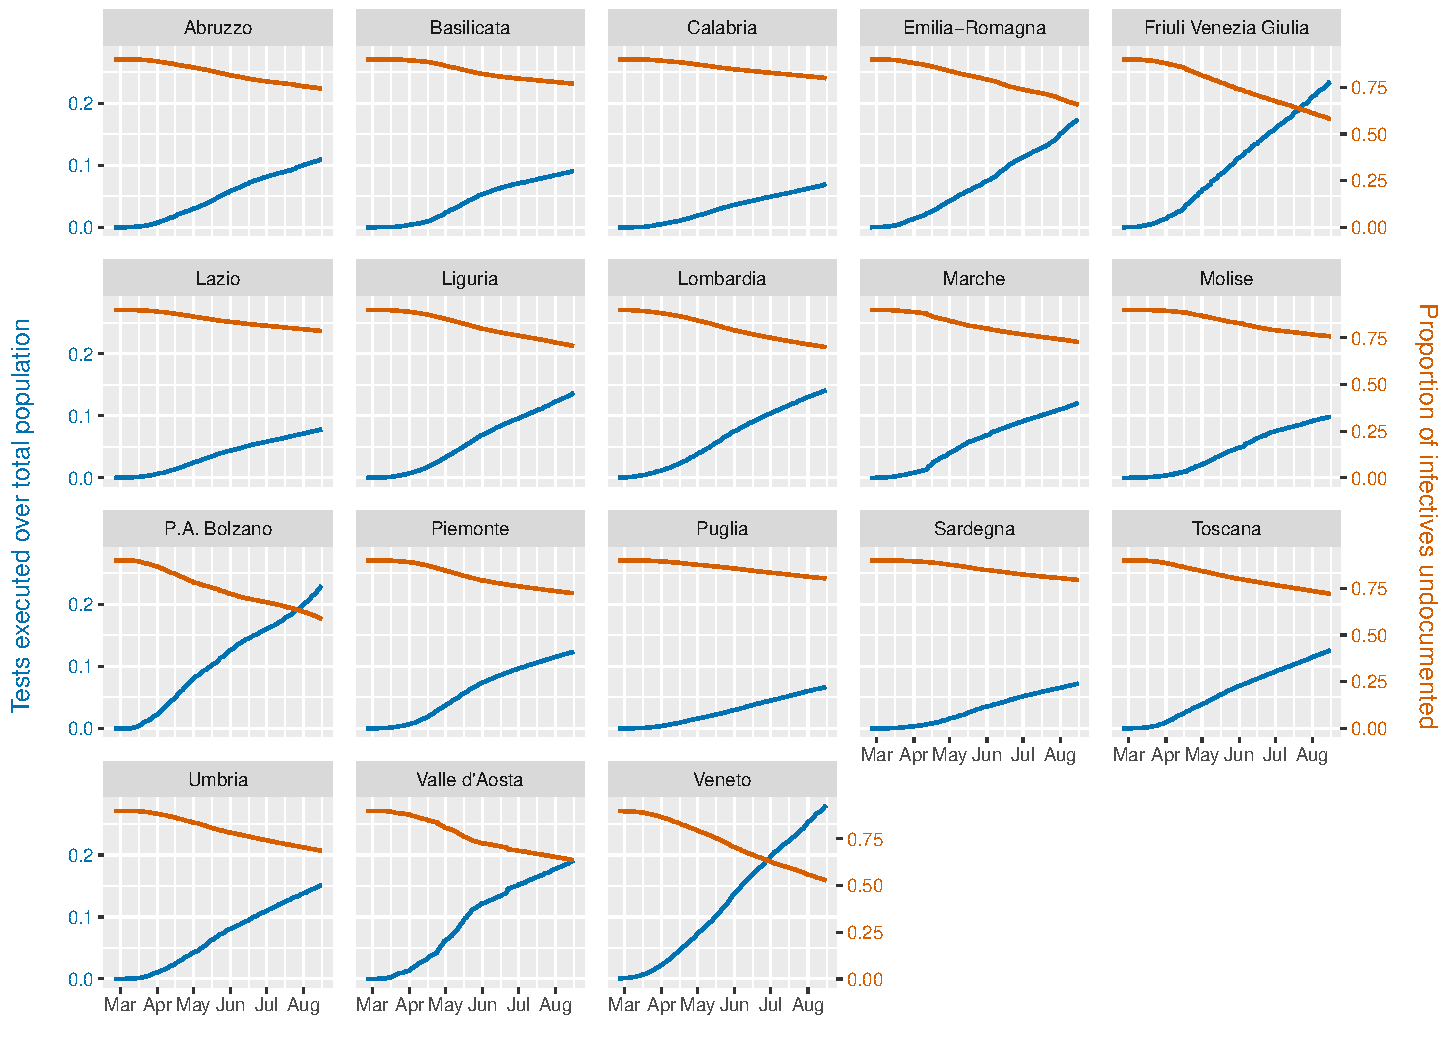
\includegraphics[width=\textwidth]{output/tamponiprop_vs_ft.pdf}
	    \caption{Total number of people tested over the total population ($TC_{r,t} / N_{r,t}$) versus proportion of infectives that are documented $f_{r,t}(\gamma)$}
	    \label{fig:tamponiprop_versus_ft}
	\end{figure}
	
	In Figure \ref{fig:tamponiprop_versus_ft}, we can see that the pattern of the relationship between the two variables is similar over time for different groups of regions. Importantly, we note that the proportion of infectives that go undocumented decreases over time. This is logical because the testing capacity increases over time and we have assumed a monotonic relationship. \\
	
	For illustration purposes, we now give an example of the impact of this modelling method. We present the number of infectives at three time points for three regions in Table \ref{tab:f_t_over_time}.
	
	\begin{table}[H]
		\centering
		\caption{Impact of modelling undocumented infectives over time. The quadratic specification with $\gamma = 0.7$ is used.}
		\label{tab:f_t_over_time}
		\begin{tabular}{llllllllllll}
		    \toprule 
                     & \multicolumn{3}{c}{Calabria} && \multicolumn{3}{c}{Lombardy} && \multicolumn{3}{c}{Veneto} \\
                     \cmidrule{2-4}\cmidrule{6-8}\cmidrule{10-12}
                     & $DI_t$  & $f_t$   & $I_t$   && $DI_t$  & $f_t$   & $I_t$    && $DI_t$  & $f_t$  & $I_t$   \\ \midrule
            April 1  & 669     & 10.8\%  & 6,448   && 44,601  & 11.8\%  & 409,003  && 9,592   & 13.4\% & 82,106  \\
            June 1   & 1,158   & 15.4\%  & 10,670  && 88,846  & 21.0\%  & 717,289  && 19,121  & 29.5\% & 139,610 \\
            August 1 & 1,269   & 19.2\%  & 11,291  && 96,102  & 28.5\%  & 747,691  && 20,133  & 44.2\% & 142,111 \\ \bottomrule
        \end{tabular}
	\end{table}
	
	Table \ref{tab:f_t_over_time} shows us that the impact of the proportion of documented infectives $f_t$ differs over the regions. We chose Calabria, Lombardy, and Veneto because these regions vary in the proportional amount of tests executed, leading to different profiles in $f_t$. We can see this profile in Figure \ref{fig:tamponiprop_versus_ft} as well. When the amount of tests executed grows less steeply, as is the case in Calabria, the number of undocumented infectives in society grows stronger. On the other hand, for a region that invests heavily in testing, such as Veneto, the undocumented infectives are less pronounced. For example, consider the changes in Calabria and Veneto from June 1 to August 1. For Calabria, the growth in the documented infectives accounted for only 17.87\% of the total growth in infectives. In contrast, in Veneto the growth in the documented infectives accounted for 40.46\% of the total growth. Of course, Lombardy finds itself in the middle, where documented infectives make up 23.87\% of the total growth. Hence, our method correctly incorporates the intuition that a higher testing capacity leads to more infectives being documented. \\
	
	Using the specification of undocumented infectives, we can now adapt the models \eqref{eq:model_within} and \eqref{eq:model_within_between} \todo[backgroundcolor=green!40]{TODO: Discrete SIR model} to include these undocumented infectives. Let us take the within-region spread model \eqref{eq:model_within} as an example. Recall that this model was given as
	    \begin{equation*}
		    \Delta Y_{r,t} = \beta_{within}\Delta Y_{r,t-\tau}S_{r,t-\tau} + \delta X_{r,t} + \eta_{r,t}.
	    \end{equation*}
	Using that $\Delta Y_{r,t} = \frac{DI_{r,t}}{f_{r,t}(\gamma)} - \frac{DI_{r,t-1}}{f_{r,t-1}(\gamma)}$, this becomes
	    \begin{equation} \label{eq:model_within_undocumented}
		    \frac{DI_{r,t}}{f_{r,t}(\gamma)} - \frac{DI_{r,t-1}}{f_{r,t-1}(\gamma)} = \beta_{within}\left(\frac{DI_{r,t-\tau}}{f_{r,t-\tau}(\gamma)} - \frac{DI_{r,t-\tau-1}}{f_{r,t-\tau-1}(\gamma)}\right)S_{r,t-\tau} + \delta X_{r,t} + \eta_{r,t}.
	    \end{equation}
	We can rewrite \eqref{eq:model_within_undocumented} as follows
	    \begin{equation*}
	       DI_{r,t} = f_{r,t}(\gamma)\left(\beta_{within}\left(\frac{DI_{r,t-\tau}}{f_{r,t-\tau}(\gamma)} - \frac{DI_{r,t-\tau-1}}{f_{r,t-\tau-1}(\gamma)}\right)S_{r,t-\tau} + \frac{DI_{r,t-1}}{f_{r,t-1}(\gamma)} + \delta X_{r,t} + \eta_{r,t}\right).
	    \end{equation*}
	    
	The moment conditions that then need to hold are:
	    \begin{align*}
	        & E\left[ \eta_{r,t}f_{r,t}(\gamma) \left( \beta_{within}\left(\frac{DI_{r,t-\tau}}{f_{r,t-\tau}(\gamma)} - \frac{DI_{r,t-\tau-1}}{f_{r,t-\tau-1}(\gamma)}\right)S_{r,t-\tau} + \frac{DI_{r,t-1}}{f_{r,t-1}(\gamma)} + \delta X_{r,t} \right) \right] = 0 \\
	        \iff & f_{r,t}(\gamma) E\left[ \eta_{r,t}\left( \beta_{within}\left(\frac{DI_{r,t-\tau}}{f_{r,t-\tau}(\gamma)} - \frac{DI_{r,t-\tau-1}}{f_{r,t-\tau-1}(\gamma)}\right)S_{r,t-\tau} + \frac{DI_{r,t-1}}{f_{r,t-1}(\gamma)} + \delta X_{r,t} \right) \right] = 0.
	    \end{align*}
	
	Since $f_{r,t}(\gamma)$ is simply a scaling function, regardless of the chosen parameter, it has no influence on the dependence between the error and the regressors. As such, it can be taken out of the expectation term. Subsequently, we can divide both sides of the equation by $f_{r,t}(\gamma)$ to obtain the following moment condition:
	    \begin{equation} \label{eq:model_within_undocumented_moments}
	        E\left[ \eta_{r,t}\left( \beta_{within}\left(\frac{DI_{r,t-\tau}}{f_{r,t-\tau}(\gamma)} - \frac{DI_{r,t-\tau-1}}{f_{r,t-\tau-1}(\gamma)}\right)S_{r,t-\tau} + \frac{DI_{r,t-1}}{f_{r,t-1}(\gamma)} + \delta X_{r,t} \right) \right] = 0.
	    \end{equation}
	
	Just like in Section \ref{sec:model_within}, we make the assumption that the idiosyncratic error $\eta_{r,t}$ is uncorrelated with the regressors in the tensor $X_{r,t}$. That is, we assume that $E\left[\eta_{r,t} \,\middle|\, X_{r,t}\right] = 0$. Now note that there are two additional terms to consider, namely the relation between $\eta_{r,t}$ and $\left(\frac{DI_{r,t-\tau}}{f_{r,t-\tau}(\gamma)} - \frac{DI_{r,t-\tau-1}}{f_{r,t-\tau-1}(\gamma)}\right)S_{r,t-\tau}$ as well as between $\eta_{r,t}$ and $\frac{DI_{r,t-1}}{f_{r,t-1}(\gamma)}$. The reason why we assume that $E\left[\eta_{r,t} ~\middle|\, \left(\frac{DI_{r,t-\tau}}{f_{r,t-\tau}(\gamma)} - \frac{DI_{r,t-\tau-1}}{f_{r,t-\tau-1}(\gamma)}\right)S_{r,t-\tau}\right] = 0$ is for the same reason as in Section \ref{sec:model_within}, namely that for a large enough lag $\tau$, the error is not correlated with past data at that lag. That is, the people that are classified as infectives at time $t-\tau$ do not have an effect on the error that we make when considering the infectives at time $t$ under a correct model specification. This is independent of the scaling functions $f_{r,t-\tau}(\gamma)$ and $f_{r,t-\tau-1}(\gamma)$ as these are constructed without the past infectives in mind. \\
	
	The issue may come when we consider the condition $E\left[\eta_{r,t} \,\middle|\,  \frac{DI_{r,t-1}}{f_{r,t-1}(\gamma)}\right] = 0$. Again, this is not due to the scaling function $f_{r,t-1}(\gamma)$ but when considering the term $DI_{r,t-1}$. However, recall that the error $\eta_{r,t}$ is made when predicting the amount of infectives at time $t$. In Section \ref{sec:model_within}, we have explained that there is a latent period during which an infected person is not able to infect others yet. As such, when considering only a one-period difference, there should be no correlation between $\eta_{r,t}$ and $DI_{r,t-1}$. Consequently, the scaling of the infectives by using our functional form, has no additional impact on the moment conditions. A similar logic applies to the moment conditions for \eqref{eq:model_within_between}. Therefore, we assume that the moment conditions hold, even when modelling undocumented infectives according to the method explained in this section. \todo[backgroundcolor=green!40]{TODO: Discrete SIR}
	
	\newpage
	\section{Results} \label{sec:results}
	In this section, we present the results from the models as presented in Section \ref{sec:methodology}. When we speak of statistical significance without specifying a significance level, a level of 0.05 is implied. In Section \ref{subsec:results_within}, we discuss the results for the within-region spread model. Subsequently, Section \ref{subsec:results_within_between} discusses the results for the within and between-region spread model. For the models in Sections \ref{subsec:results_within} and \ref{subsec:results_within_between}, \textcite{adda2016economic} explains that the estimated coefficients can be interpreted as the marginal effects of a change in the infection rate on the future infection rate when the entire population is susceptible to the disease. We will explain more on this interpretation in the respective section. After discussing the models by \textcite{adda2016economic}, we present the results from estimating the discrete SIR model in Section \ref{subsec:results_discrete_sir}.
	
	\newpage
	\section{Conclusion} \label{sec:conclusion}
	% Conclusions
	
	\newpage
	\section{Future research} \label{sec:future_research}
	% The third assumption that the SIR model makes is that there is a constant rate of change at which infectives recover or decease. =>  The fuller hospitals are, the more people will likely decease.
	%  For simplicity’s sake, we assume that lambda = 0. => Look into cases where lambda is not equal to 0.
	
	% GMR: If more daily travel data is known with absolute numbers, this could be incorporated more easily.

    % On between region: only take into account close regions or with close economic ties, if data is available
	
	% Spatial Panel Data can be applied if weights are constructed
	
	%Bibliography
	\newpage
	\printbibliography
	
	\newpage\appendix
	
	\begin{appendices}
	    \section{Abbreviations}\label{app:abbreviations}
	
	    The tables in this appendix present commonly used abbreviations in this thesis, including the regional abbreviations.
	    
	    \begin{xltabular}{\textwidth}{lXX}
    		\caption{Abbreviations for the Italian regions.}
    		\label{tab:abbreviations_regions}\\
    		\toprule
    		Abbreviation & Italian name & English name \\* \midrule
    		\endfirsthead
    		
    		\multicolumn{3}{c}{{\bfseries Table \thetable\ continued from previous page}} \\
    		\toprule
    		Abbreviation & Italian name & English name \\* \midrule
    		\endhead
    		
    		\bottomrule
    		\multicolumn{3}{c}{{\bfseries Table \thetable\ continues on next page}}
    		\endfoot
    		
    		\endlastfoot
    		
            ABR & Abruzzo & Abruzzo \\ 
            BAS & Basilicata & Basilicata \\ 
            BZ & Alto Adige or Provincia Autonoma di Bolzano/Bozen & South Tyrol or Province of Bolzano \\ 
            CAL & Calabria & Calabria \\ 
            CAM & Campania & Campania \\
            EMR & Emilia-Romagna & Emilia-Romagna \\ 
            FVG & Friuli Venezia Giulia & Friuli Venezia Giulia \\
            LAZ & Lazio & Lazio \\ 
            LIG & Liguria & Liguria \\ 
            LOM & Lombardia & Lombardy \\ 
            MAR & Marche & Marche \\ 
            MOL & Molise & Molise \\ 
            PIE & Piemonte & Piedmont \\ 
            PUG & Puglia & Apulia \\ 
            SAR & Sardegna & Sardinia \\ 
            SIC & Sicilia & Sicily \\ 
            TN  & Trentino or Provincia Autonoma di Trento & Trentino or Province of Trento \\ 
            TOS & Toscana & Tuscany \\ 
            UMB & Umbria & Umbria \\ 
            VDA & Valle d'Aosta/Vallée d'Aoste & Aosta Valley \\ 
            VEN & Veneto & Veneto \\* \bottomrule
    	\end{xltabular}
	    
	    \begin{xltabular}{\textwidth}{lXX}
    		\caption{Commonly used abbreviations in this thesis.}
    		\label{tab:abbreviations_misc}\\
    		\toprule
    		Abbreviation & Full name & Defined in... \\* \midrule
    		\endfirsthead
    		
    		\multicolumn{3}{c}{{\bfseries Table \thetable\ continued from previous page}} \\
    		\toprule
    		Abbreviation & Full name & Defined in... \\* \midrule
    		\endhead
    		
    		\bottomrule
    		\multicolumn{3}{c}{{\bfseries Table \thetable\ continues on next page}}
    		\endfoot
    		
    		\endlastfoot
    		
            SARS-CoV-2 & Severe Acute Respiratory Syndrome Coronavirus 2 & Section \ref{sec:introduction} \\ 
            COVID-19 & Coronavirus Disease 2019 & Section \ref{sec:introduction} \\
            NUTS & Nomenclature des Unités Territoriales Statistiques & Section \ref{sec:problem_description} \\
            SIR model & Standard Inflammatory Response model & Section \ref{sec:sir_model} \\
            OLS & Ordinary Least Squares & Section \ref{sec:model_within} \\
            AIC & Akaike Information Criterion & Section \ref{sec:model_selection} \\
            BIC & Bayesian Information Criterion & Section \ref{sec:model_selection}  \\
            POLS & Pooled Ordinary Least Squares & Section \ref{subsec:discrete_sir_panel} \\
            RE & Random Effects & Section \ref{subsec:discrete_sir_panel} \\* \bottomrule
    	\end{xltabular}
    	
		\section{Tables} \label{app:tables}
		
		\subsection{Results from Within-Region Spread Model}
		In Section \ref{subsec:results_within}, we presented the results from the within-region spread model \eqref{eq:model_within}:
		    \begin{equation*}
        		\Delta Y_{r,t} = \beta_{within}\Delta Y_{r,t-\tau}S_{r,t-\tau} + \delta X_{r,t} + \eta_{r,t}.
        	\end{equation*}
        	
    	This appendix contains additional tables with results for this model. As is the case for Section \ref{subsec:results_within}, we use the last 100 observations.
    	
    	\begin{longtable}{@{}lcccc@{}}
    		\caption{Estimates from Within-Region Spread Model per region without model selection. Estimates are given with $t$-statistics in parentheses. Data spans May 9 till August 16, 2020 (100 days). Undocumented infectives are modelled using the quadratic specification with $\gamma = 0.7$ and $f^{min}=0.1$.}
    		\label{tab:results_within}\\
    		\toprule
    		                & \multicolumn{2}{c}{Regular model} & \multicolumn{2}{c}{Modelling undocumented infectives} \\
    		                \cmidrule(lr){2-3}
                            \cmidrule(lr){4-5}
    		Region          & $\beta_{within}$ & Weekend & $\beta_{within}$ & Weekend \\* \midrule
    		\endfirsthead
    		
    		\multicolumn{5}{c}{{\bfseries Table \thetable\ continued from previous page}} \\
    		\toprule
    		                & \multicolumn{2}{c}{Regular model} & \multicolumn{2}{c}{Modelling undocumented infectives} \\
    		                \cmidrule(lr){2-3}
                            \cmidrule(lr){4-5}
    		Region          & $\beta_{within}$ & Weekend & $\beta_{within}$ & Weekend \\* \midrule
    		\endhead
    		
    		\bottomrule
    		\multicolumn{5}{c}{{\bfseries Table \thetable\ continues on next page}}
    		\endfoot
    		
    		\multicolumn{5}{c}{Significance levels: * = 0.1 ** = 0.05, *** = 0.01}
    		\endlastfoot
    		
            National & 0.886*** & 11.604 & 0.863*** & 36.761 \\ 
             & (21.493) & (0.369) & (23.925) & (0.261) \\ 
            ABR & 0.463*** & 2.715** & 0.494*** & 12.934** \\ 
             & (5.081) & (2.084) & (5.854) & (2.160) \\ 
            BAS & 0.076 & 0.482 & 0.081 & 2.551 \\ 
             & (0.730) & (0.571) & (0.773) & (0.656) \\ 
            BZ & 0.460*** & 2.111*** & 0.386*** & 6.532*** \\ 
             & (5.172) & (3.566) & (4.541) & (3.819) \\ 
            CAL & 0.297*** & 2.176** & 0.268** & 12.544*** \\ 
             & (2.689) & (2.600) & (2.499) & (2.755) \\ 
            EMR & 0.737*** & 14.644*** & 0.703*** & 54.997*** \\ 
             & (13.515) & (3.441) & (14.736) & (3.329) \\ 
            FVG & 0.719*** & 1.106 & 0.739*** & 2.858 \\ 
             & (9.005) & (1.465) & (11.080) & (1.241) \\ 
            LAZ & 0.840*** & 6.783*** & 0.795*** & 38.587*** \\ 
             & (13.863) & (2.705) & (13.695) & (2.712) \\ 
            LIG & 0.816*** & $-0.501$ & 0.835*** & $-4.795$ \\ 
             & (12.860) & ($-0.172$) & (15.253) & ($-0.358$) \\ 
            LOM & 0.797*** & 7.588 & 0.776*** & 38.615 \\ 
             & (13.165) & (0.303) & (12.987) & (0.300) \\ 
            MAR & 0.576*** & 2.297* & 0.572*** & 11.050** \\ 
             & (7.694) & (1.836) & (9.102) & (2.055) \\ 
            MOL & 0.343*** & 0.283 & 0.344*** & 1.358 \\ 
             & (6.679) & (0.704) & (7.829) & (0.598) \\ 
            PIE & 0.814*** & $-1.842$ & 0.798*** & $-14.985$ \\ 
             & (16.951) & ($-0.376$) & (17.718) & ($-0.607$) \\ 
            PUG & 0.639*** & 2.023* & 0.586*** & 13.379* \\ 
             & (9.129) & (1.678) & (9.265) & (1.920) \\ 
            SAR & 0.342*** & 0.785 & 0.329*** & 4.468 \\ 
             & (3.496) & (1.245) & (3.493) & (1.400) \\ 
            TOS & 0.735*** & 6.130*** & 0.702*** & 26.588*** \\ 
             & (10.869) & (3.411) & (11.061) & (3.355) \\  
            UMB & 0.607*** & 1.094** & 0.506*** & 4.070** \\ 
             & (5.918) & (2.498) & (5.059) & (2.501) \\ 
            VDA & 0.197** & 0.381 & 0.281*** & 1.189 \\ 
             & (2.051) & (1.350) & (3.127) & (1.248) \\ 
            VEN & 0.652*** & 9.808 & 0.652*** & 22.618 \\ 
             & (6.866) & (1.529) & (7.784) & (1.531) \\* \bottomrule
    	\end{longtable}
		
		\begin{longtable}{@{}lcccc@{}}
    		\caption{Estimates from Within-Region Spread Model per region with model selection by AIC versus BIC. Estimates are given with $t$-statistics in parentheses. Data spans May 9 till August 16, 2020 (100 days). Undocumented infectives are modelled using the quadratic specification with $\gamma = 0.7$ and $f^{min}=0.1$.}
    		\label{tab:model1_aic_vs_bic}\\
    		\toprule
    		                & \multicolumn{2}{c}{Model selection with AIC} & \multicolumn{2}{c}{Model selection with BIC} \\
    		                \cmidrule(lr){2-3}
                            \cmidrule(lr){4-5}
    		Region          & $\beta_{within}$ & Weekend & $\beta_{within}$ & Weekend \\* \midrule
    		\endfirsthead
    		
    		\multicolumn{5}{c}{{\bfseries Table \thetable\ continued from previous page}} \\
    		\toprule
    		                & \multicolumn{2}{c}{Model selection with AIC} & \multicolumn{2}{c}{Model selection with BIC} \\
    		                \cmidrule(lr){2-3}
                            \cmidrule(lr){4-5}
    		Region          & $\beta_{within}$ & Weekend & $\beta_{within}$ & Weekend \\* \midrule
    		\endhead
    		
    		\bottomrule
    		\multicolumn{5}{c}{{\bfseries Table \thetable\ continues on next page}}
    		\endfoot
    		
    		\multicolumn{5}{c}{Significance levels: * = 0.1 ** = 0.05, *** = 0.01}
    		\endlastfoot
    		
            National & 0.867*** &  & 0.867*** &  \\ 
             & (26.564) &  & (26.564) &  \\ 
            ABR & 0.494*** & 12.934** & 0.494*** & 12.934** \\ 
             & (5.854) & (2.160) & (5.854) & (2.160) \\ 
            BAS & 0.095 & & 0.095 &  \\ 
             & (0.933) &  & (0.933) &  \\ 
            BZ & 0.386*** & 6.532*** & 0.386*** & 6.532*** \\ 
             & (4.541) & (3.819) & (4.541) & (3.819) \\ 
            CAL & 0.269** & 12.544*** & 0.269** & 12.544*** \\ 
             & (2.499) & (2.755) & (2.499) & (2.755) \\ 
            EMR & 0.703*** & 54.997*** & 0.703*** & 54.997*** \\ 
             & (14.736) & (3.329) & (14.736) & (3.329) \\ 
            FVG & 0.772*** &  & 0.772*** &  \\ 
             & (12.629) &  & (12.629) &  \\ 
            LAZ & 0.795*** & 38.587*** & 0.795*** & 38.587*** \\ 
             & (13.695) & (2.712) & (13.695) & (2.712) \\ 
            LIG & 0.828*** &  & 0.828*** &  \\ 
             & (16.459) &  & (16.459) &  \\ 
            LOM & 0.783*** &  & 0.783*** &  \\ 
             & (14.183) &  & (14.183) &  \\ 
            MAR & 0.572*** & 11.050** & 0.608*** &  \\ 
             & (9.102) & (2.055) & (9.920) &  \\ 
            MOL & 0.348*** &  & 0.348*** &  \\ 
             & (8.064) &  & (8.064) &  \\ 
            PIE & 0.788*** &  & 0.788*** &  \\ 
             & (18.917) &  & (18.917) &  \\ 
            PUG & 0.586*** & 13.379* & 0.624*** &  \\ 
             & (9.265) & (1.920) & (10.248) &  \\ 
            SAR & 0.361*** &  & 0.361*** &  \\ 
             & (3.924) &  & (3.924) &  \\ 
            TOS & 0.702*** & 26.588*** & 0.702*** & 26.588*** \\ 
             & (11.061) & (3.355) & (11.061) & (3.355) \\ 
            UMB & 0.506*** & 4.070** & 0.506*** & 4.070** \\ 
             & (5.059) & (2.501) & (5.059) & (2.501) \\ 
            VDA & 0.298*** &  & 0.298*** &  \\ 
             & (3.346) &  & (3.346) &  \\ 
            VEN & 0.652*** & 22.618 & 0.699*** &  \\ 
             & (7.784) & (1.531) & (8.933) &  \\* \bottomrule
        \end{longtable}
		
		\subsection{Results from Within and Between-Region Spread Model}\label{sapp:results_within_between}
		In Section \ref{subsec:results_within_between}, we presented the results from the within and between-region spread model \eqref{eq:model_within_between}:
		    \begin{equation*}
        		\Delta Y_{r,t} = \beta_{within}\Delta Y_{r,t-\tau} S_{r,t-\tau} + \beta_{between}S_{r,t-\tau}\sum_{c \in R \setminus r} \Delta Y_{c, t-\tau} + \delta X_{r,t} + \eta_{r,t}
        	\end{equation*}
        
        This appendix contains additional tables with results for this model. As is the case for Section \ref{subsec:results_within_between}, we use the last 100 observations.
		
% 		\begin{landscape}
		\begin{longtable}{@{}lcccccc@{}}
    		\caption{Estimates from Within and Between-Region Spread Model per region without model selection. Estimates are given with $t$-statistics in parentheses. Data spans May 9 till August 16, 2020 (100 days). Undocumented infectives are modelled using the quadratic specification with $\gamma = 0.7$ and $f^{min}=0.1$.}
    		\label{tab:results_within_between}\\
    		\toprule
    		                & \multicolumn{3}{c}{Regular model} & \multicolumn{3}{c}{Modelling undocumented infectives} \\
    		                \cmidrule(lr){2-4}
                            \cmidrule(lr){5-7}
    		Region          & $\beta_{within}$ & $\beta_{between}$ & Weekend & $\beta_{within}$ & $\beta_{between}$ & Weekend \\* \midrule
    		\endfirsthead
    		
    		\multicolumn{7}{c}{{\bfseries Table \thetable\ continued from previous page}} \\
    		\toprule
    		                & \multicolumn{3}{c}{Regular model} & \multicolumn{3}{c}{Modelling undocumented infectives} \\
    		                \cmidrule(lr){2-4}
                            \cmidrule(lr){5-7}
    		Region          & $\beta_{within}$ & $\beta_{between}$ & Weekend & $\beta_{within}$ & $\beta_{between}$ & Weekend \\* \midrule
    		\endhead
    		
    		\bottomrule
    		\multicolumn{7}{c}{{\bfseries Table \thetable\ continues on next page}}
    		\endfoot
    		
    		\multicolumn{7}{c}{Significance levels: * = 0.1 ** = 0.05, *** = 0.01}
    		\endlastfoot
    		
            ABR & 0.217* & $7.804 \times 10^{-3}$*** & 1.052 & 0.194* & $8.395 \times 10^{-3}$*** & 6.299 \\ 
             & (1.963) & (3.565) & (0.801) & (1.850) & (4.237) & (1.099) \\ 
            BAS & 0.059 & $1.580 \times 10^{-3}$ & $-0.087$ & 0.065 & $1.295 \times 10^{-3}$ & 0.502 \\ 
             & (0.558) & (1.299) & ($-0.092$) & (0.618) & (1.213) & (0.119) \\ 
            BZ & 0.399*** & $1.213 \times 10^{-3}$ & 1.784*** & 0.325*** & $6.790 \times 10^{-4}$ & 5.771*** \\ 
             & (3.968) & (1.288) & (2.777) & (3.368) & (1.303) & (3.204) \\ 
            CAL & 0.232* & $1.979 \times 10^{-3}$ & 1.569* & 0.208* & $1.969 \times 10^{-3}$ & 9.985** \\ 
             & (1.985) & (1.588) & (1.717) & (1.829) & (1.524) & (2.070) \\ 
            EMR & 0.612*** & 0.017 & 13.610*** & 0.517*** & 0.020** & 52.882*** \\ 
             & (6.499) & (1.626) & (3.190) & (5.542) & (2.308) & (3.268) \\ 
            FVG & 0.366*** & $5.747 \times 10^{-3}$*** & 0.499 & 0.231** & $5.395 \times 10^{-3}$*** & 0.971 \\ 
             & (3.188) & (4.028) & (0.697) & (2.182) & (5.741) & (0.481) \\ 
            LAZ & 0.535*** & 0.021*** & 5.179** & 0.451*** & 0.027*** & 33.375** \\ 
             & (5.524) & (3.866) & (2.178) & (4.951) & (4.634) & (2.577) \\ 
            LIG & 0.371*** & 0.037*** & $-4.824$* & 0.366*** & 0.038*** & $-21.002$* \\ 
             & (4.474) & (6.893) & ($-1.954$) & (4.884) & (7.650) & ($-1.948$) \\ 
            LOM & 0.517*** & 0.408*** & $-26.370$ & 0.328*** & 0.639*** & $-151.305$ \\ 
             & (6.303) & (4.584) & ($-1.101$) & (3.808) & (6.410) & ($-1.351$) \\ 
            MAR & 0.297*** & $8.745 \times 10^{-3}$*** & 0.525 & 0.283*** & $8.571 \times 10^{-3}$*** & 3.831 \\ 
             & (2.722) & (3.379) & (0.404) & (2.957) & (3.821) & (0.713) \\ 
            MOL & 0.249*** & $1.893 \times 10^{-3}$*** & $-0.285$ & 0.255*** & $2.097 \times 10^{-3}$*** & -1.396 \\ 
             & (4.149) & (2.788) & ($-0.649$) & (4.742) & (2.721) & ($-0.577$) \\ 
            PIE & 0.434*** & 0.068*** & $-8.761$* & 0.327*** & 0.086*** & $-43.752$* \\ 
             & (4.910) & (4.933) & ($-1.903$) & (3.508) & (5.577) & ($-1.977$) \\ 
            PUG & 0.480*** & $5.814 \times 10^{-3}$*** & 0.769 & 0.418*** & $7.016 \times 10^{-3}$*** & 7.581 \\ 
             & (5.301) & (2.663) & (0.611) & (4.808) & (2.707) & (1.071) \\ 
            SAR & 0.277*** & $1.709 \times 10^{-3}$* & 0.241 & 0.276*** & $1.351 \times 10^{-3}$ & 2.635 \\ 
             & (2.682) & (1.803) & (0.347) & (2.744) & (1.462) & (0.772) \\ 
            TOS & 0.532*** & 0.010*** & 4.567** & 0.416*** & 0.012*** & 20.546*** \\ 
             & (5.463) & (2.812) & (2.506) & (4.293) & (3.743) & (2.701) \\ 
            UMB & 0.539*** & $8.368 \times 10^{-4}$ & 0.856* & 0.406*** & $8.290 \times 10^{-4}$ & 3.089* \\ 
             & (4.575) & (1.174) & (1.78) & (3.463) & (1.606) & (1.790) \\ 
            VDA & $-0.057$ & $2.194 \times 10^{-3}$*** & $-0.330$ & $-0.054$ & $1.715 \times 10^{-3}$*** & $-1.111$ \\ 
             & ($-0.581$) & (5.119) & ($-1.151$) & ($-0.574$) & (6.171) & ($-1.249$) \\ 
            VEN & 0.573*** & 0.015 & 6.363 & 0.535*** & $8.695 \times 10^{-3}$* & 16.258 \\ 
             & (5.261) & (1.445) & (0.935) & (4.989) & (1.715) & (1.078) \\* \bottomrule
    	\end{longtable}
		
		\begin{longtable}{@{}lcccccc@{}}
    		\caption{Estimates from Within and Between-Region Spread Model per region with model selection by AIC versus BIC. Estimates are given with $t$-statistics in parentheses. Data spans May 9 till August 16, 2020 (100 days). Undocumented infectives are modelled using the quadratic specification with $\gamma = 0.7$ and $f^{min}=0.1$.}
    		\label{tab:results_within_between_aic_vs_bic}\\
    		\toprule
    		                & \multicolumn{3}{c}{Model selection with AIC} & \multicolumn{3}{c}{Model selection with BIC} \\
    		                \cmidrule(lr){2-4}
                            \cmidrule(lr){5-7}
    		Region          & $\beta_{within}$ & $\beta_{between}$ & Weekend & $\beta_{within}$ & $\beta_{between}$ & Weekend \\* \midrule
    		\endfirsthead
    		
    		\multicolumn{7}{c}{{\bfseries Table \thetable\ continued from previous page}} \\
    		\toprule
    		                & \multicolumn{3}{c}{Model selection with AIC} & \multicolumn{3}{c}{Model selection with BIC} \\
    		                \cmidrule(lr){2-4}
                            \cmidrule(lr){5-7}
    		Region          & $\beta_{within}$ & $\beta_{between}$ & Weekend & $\beta_{within}$ & $\beta_{between}$ & Weekend \\* \midrule
    		\endhead
    		
    		\bottomrule
    		\multicolumn{7}{c}{{\bfseries Table \thetable\ continues on next page}}
    		\endfoot
    		
    		\multicolumn{7}{c}{Significance levels: * = 0.1 ** = 0.05, *** = 0.01}
    		\endlastfoot
    		
            ABR & 0.201* & $8.989 \times 10^{-3}$*** &  & 0.201* & $8.989 \times 10^{-3}$*** &  \\ 
             & (1.917) & (4.711) & & (1.917) & (4.711) &  \\ 
            BAS & 0.067 & $1.345 \times 10^{-3}$ &  & 0.067 & $1.345 \times 10^{-3}$ &  \\ 
             & (0.644) & (1.382) &  & (0.644) & (1.382) &  \\ 
            BZ & 0.325*** & $6.790 \times 10^{-4}$ & 5.771*** & 0.325*** & $6.790 \times 10^{-4}$ & 5.771*** \\ 
             & (3.368) & (1.303) & (3.204) & (3.368) & (1.303) & (3.204) \\ 
            CAL & 0.208* & $1.969 \times 10^{-3}$ & 9.985** & 0.239** & $2.900 \times 10^{-3}$** &  \\ 
             & (1.829) & (1.524) & (2.070) & (2.085) & (2.354) &  \\ 
            EMR & 0.517*** & 0.020** & 52.882*** & 0.517*** & 0.020** & 52.882*** \\ 
             & (5.542) & (2.308) & (3.268) & (5.542) & (2.308) & (3.268) \\ 
            FVG & 0.235** & $5.468 \times 10^{-3}$*** &  & 0.235** & $5.468 \times 10^{-3}$*** &  \\ 
             & (2.238) & (5.922) &  & (2.238) & (5.922) &  \\ 
            LAZ & 0.451*** & 0.027*** & 33.375** & 0.451*** & 0.027*** & 33.375** \\ 
             & (4.951) & (4.634) & (2.577) & (4.951) & (4.634) & (2.577) \\ 
            LIG & 0.366*** & 0.038*** & $-21.002$* & 0.358*** & 0.036*** &  \\ 
             & (4.884) & (7.650) & ($-1.948$) & (4.711) & (7.305) &  \\ 
            LOM & 0.328*** & 0.603*** &  & 0.328*** & 0.603*** &  \\ 
             & (3.799) & (6.249) &  & (3.799) & (6.249) &  \\ 
            MAR & 0.275*** & $9.133 \times 10^{-3}$*** &  & 0.275*** & $9.133 \times 10^{-3}$*** &  \\ 
             & (2.902) & (4.361) &  & (2.902) & (4.361) &  \\ 
            MOL & 0.259*** & $1.912 \times 10^{-3}$*** &  & 0.259*** & $1.912  \times 10^{-3}$*** &  \\ 
             & (4.884) & (2.740) &  & (4.884) & (2.740) &  \\ 
            PIE & 0.327*** & 0.086*** & $-43.752$* & 0.338*** & 0.078*** &  \\ 
             & (3.508) & (5.577) & ($-1.977$) & (3.575) & (5.182) &  \\ 
            PUG & 0.418*** & $7.857 \times 10^{-3}$*** &  & 0.418*** & $7.857 \times 10^{-3}$*** &  \\ 
             & (4.799) & (3.178) &  & (4.799) & (3.178) &  \\ 
            SAR & 0.282*** & $1.613 \times 10^{-3}$* &  & 0.282*** & $1.613 \times 10^{-3}$* &  \\ 
             & (2.815) & (1.881) &  & (2.815) & (1.881) &  \\ 
            TOS & 0.416*** & 0.012*** & 20.546*** & 0.416*** & 0.012*** & 20.546*** \\ 
             & (4.293) & (3.743) & (2.701) & (4.293) & (3.743) & (2.701) \\ 
            UMB & 0.406*** & $8.290 \times 10^{-4}$ & 3.089* & 0.408*** & $1.156 \times 10^{-3}$** &  \\ 
             & (3.463) & (1.606) & (1.790) & (3.444) & (2.368) &  \\ 
            VDA & $-0.039$ & $1.569 \times 10^{-3}$*** &  & $-0.039$ & $1.569 \times 10^{-3}$*** &  \\
             & ($-0.414$) & (6.202) &  & ($-0.414$) & (6.202) &  \\ 
            VEN & 0.549*** & 0.010** &  & 0.549*** & 0.010** &  \\ 
             & (5.155) & (2.040) &  & (5.155) & (2.040) &  \\* \bottomrule
    	\end{longtable}
% 		\end{landscape}
		
		\subsection{Results for Discrete Panel Data}\label{sapp:results_discrete_sir}
		In Section \ref{subsec:results_discrete_sir}, we presented the results from the discrete SIR models
		    \todo[inline, backgroundcolor=green!40]{TODO: Insert equations}
        
        This appendix contains additional tables with results for this model. As is the case for Section \ref{subsec:results_discrete_sir}, we use the last 100 observations.
        
        \begin{landscape}
    	\begin{longtable}{@{}lccccccc@{}}
    		\caption{Estimates for the discrete SIR model per region comparing different values for the lag $\tau$. Estimates are given with $t$-statistics in parentheses. Data spans May 9 till August 16, 2020 (100 days). Undocumented infectives are not modelled. Frequency-dependent transmission is used.}
    		\label{tab:results_discrete_regional_tau}\\
    		\toprule
    		                & \multicolumn{3}{c}{$\tau = 1$} & \multicolumn{3}{c}{$\tau = 3$} \\
    		                \cmidrule(lr){2-4}
                            \cmidrule(lr){5-7}
    		Region          & $\beta$ & $\beta_{two-step}$ & $\gamma$ & $\beta$ & $\beta_{two-step}$ & $\gamma$ \\* \midrule
    		\endfirsthead
    		
    		\multicolumn{7}{c}{{\bfseries Table \thetable\ continued from previous page}} \\
    		\toprule
    		                & \multicolumn{3}{c}{$\tau = 1$} & \multicolumn{3}{c}{$\tau = 3$} \\
    		                \cmidrule(lr){2-4}
                            \cmidrule(lr){5-7}
    		Region          & $\beta$ & $\beta_{two-step}$ & $\gamma$ & $\beta$ & $\beta_{two-step}$ & $\gamma$ \\* \midrule
    		\endhead
    		
    		\bottomrule
    		\multicolumn{7}{c}{{\bfseries Table \thetable\ continues on next page}}
    		\endfoot
    		
    		\multicolumn{7}{c}{Significance levels: * = 0.1 ** = 0.05, *** = 0.01}
    		\endlastfoot
            National & $4.976 \times 10^{-5}$*** & 0.011*** & $3.626 \times 10^{-5}$*** & $5.039 \times 10^{-5}$*** & $1.142 \times 10^{-3}$*** & $3.626 \times 10^{-5}$*** \\  
            National\_zvals & (6.544) & (31.512) & (5.571) & (6.455) & (30.748) & (5.571) \\ 
            ABR & $6.890 \times 10^{-3}$*** & $7.247 \times 10^{-3}$*** & $5.749 \times 10^{-3}$*** & $6.907 \times 10^{-3}$*** & $7.265 \times 10^{-3}$*** & $5.749 \times 10^{-3}$*** \\ 
            ABR\_zvals & (8.637) & (38.656) & (7.216) & (8.629) & (38.376) & (7.216) \\ 
            BAS & $6.917 \times 10^{-3}$*** & $6.962 \times 10^{-3}$*** & $4.418 \times 10^{-3}$*** & $6.962 \times 10^{-3}$*** & $6.998 \times 10^{-3}$*** & $4.418 \times 10^{-3}$*** \\ 
            BAS\_zvals & (5.234) & (6.904) & (5.221) & (5.243) & (6.905) & (5.221) \\ 
            BZ & $3.248 \times 10^{-3}$*** & $3.258 \times 10^{-3}$*** & $2.297 \times 10^{-3}$***  & $3.253 \times 10^{-3}$*** & $3.263 \times 10^{-3}$*** & $2.297 \times 10^{-3}$*** \\ 
            BZ\_zvals & (9.265) & (29.559) & (7.005) & (9.261) & (29.482) & (7.005) \\ 
            CAL & $7.467 \times 10^{-3}$*** & $7.522 \times 10^{-3}$*** & $5.609 \times 10^{-3}$*** & $7.495 \times 10^{-3}$*** & $7.545 \times 10^{-3}$*** & $5.609 \times 10^{-3}$*** \\ 
            CAL\_zvals & (8.048) & (22.664) & (6.148) & (8.049) & (22.582) & (6.148) \\ 
            EMR & $4.501 \times 10^{-3}$*** & $4.730 \times 10^{-3}$*** & $3.329 \times 10^{-3}$*** & $4.511 \times 10^{-3}$*** & $4.742 \times 10^{-3}$*** & $3.329 \times 10^{-3}$*** \\  
            EMR\_zvals & (11.873) & (67.727) & (9.116) & (11.857) & (67.315) & (9.116) \\ 
            FVG & $4.339 \times 10^{-3}$*** & $4.457 \times 10^{-3}$*** & $3.255 \times 10^{-3}$*** & $4.344 \times 10^{-3}$*** & $4.466 \times 10^{-3}$*** & $3.255 \times 10^{-3}$*** \\ 
            FVG\_zvals & (7.690) & (39.723) & (6.287) & (7.675) & (39.542) & (6.287) \\ 
            LAZ & $8.194 \times 10^{-3}$*** & $8.570 \times 10^{-3}$*** & $6.036 \times 10^{-3}$*** & $8.227 \times 10^{-3}$*** & $8.609 \times 10^{-3}$*** & $6.036 \times 10^{-3}$*** \\ 
            LAZ\_zvals & (6.581) & (53.328) & (4.813) & (6.5723) & (52.7361) & (4.81285) \\ 
            LIG & $5.978 \times 10^{-3}$*** & $6.271 \times 10^{-3}$*** & $4.487 \times 10^{-3}$*** & $5.976 \times 10^{-3}$*** & $6.288 \times 10^{-3}$*** & $4.487 \times 10^{-3}$*** \\ 
            LIG\_zvals & (7.476) & (33.236) & (6.626) & (7.431) & (32.916) & (6.627) \\ 
            LOM & $6.210 \times 10^{-3}$*** & $6.415 \times 10^{-3}$*** & $4.565 \times 10^{-3}$*** & $6.219 \times 10^{-3}$*** & $6.434 \times 10^{-3}$*** & $4.565 \times 10^{-3}$*** \\ 
            LOM\_zvals & (10.809) & (37.672) & (9.531) & (10.760) & (37.313) & (9.531) \\ 
            MAR & $6.097 \times 10^{-3}$*** & $6.141 \times 10^{-3}$*** & $5.263 \times 10^{-3}$*** & $6.100 \times 10^{-3}$*** & $6.149 \times 10^{-3}$*** & $5.263 \times 10^{-3}$*** \\ 
            MAR\_zvals & (7.691) & (53.351) & (6.883) & (7.678) & (52.948) & (6.883) \\ 
            MOL & 0.010*** & 0.010*** & $6.753 \times 10^{-3}$*** & $9.954 \times 10^{-3}$*** & 0.010*** & $6.753 \times 10^{-3}$*** \\
            MOL\_zvals & (6.835) & (11.366) & (6.638) & (6.689) & (11.073) & (6.638) \\ 
            PIE & $6.309 \times 10^{-3}$*** & $6.566 \times 10^{-3}$*** & $5.313 \times 10^{-3}$*** & $6.306 \times 10^{-3}$*** & $6.578 \times 10^{-3}$*** & $5.313 \times 10^{-3}$*** \\ 
            PIE\_zvals & (8.138) & (48.683) & (7.794) & (8.099) & (48.057) & (7.794) \\ 
            PUG & $7.622 \times 10^{-3}$*** & $7.862 \times 10^{-3}$*** & $6.513 \times 10^{-3}$*** & $7.634 \times 10^{-3}$*** & $7.879 \times 10^{-3}$*** & $6.513 \times 10^{-3}$*** \\ 
            PUG\_zvals & (8.617) & (47.630) & (7.346) & (8.600) & (47.102) & (7.346) \\ 
            SAR & $5.487 \times 10^{-3}$*** & $5.594 \times 10^{-3}$*** & $5.374 \times 10^{-3}$*** & $5.499 \times 10^{-3}$*** & $5.604 \times 10^{-3}$*** & $4.374 \times 10^{-3}$*** \\ 
            SAR\_zvals & (6.843) & (24.746) & (5.531) & (6.841) & (24.619) & (5.531) \\ 
            TOS & $5.704 \times 10^{-3}$*** & $5.902 \times 10^{-3}$*** & $4.785 \times 10^{-3}$*** & $5.709 \times 10^{-3}$*** & $5.913 \times 10^{-3}$*** & $4.785 \times 10^{-3}$*** \\ 
            TOS\_zvals & (7.043) & (57.604) & (6.124) & (7.031) & (57.242) & (6.124) \\ 
            UMB & $2.160 \times 10^{-3}$*** & $2.222 \times 10^{-3}$*** & $1.217 \times 10^{-3}$*** & $2.161 \times 10^{-3}$*** & $2.223 \times 10^{-3}$*** & $1.217 \times 10^{-3}$*** \\ 
            UMB\_zvals & (8.453) & (13.646) & (6.331) & (8.432) & (13.598) & (6.331) \\ 
            VDA & $2.017 \times 10^{-3}$*** & $2.076 \times 10^{-3}$*** & $1.489 \times 10^{-3}$*** & $2.017 \times 10^{-3}$*** & $2.077 \times 10^{-3}$*** & $1.489 \times 10^{-3}$*** \\ 
            VDA\_zvals & (6.145) & (16.797) & (5.591) & (6.135) & (16.782) & (5.591) \\ 
            VEN & $4.781 \times 10^{-3}$*** & $5.018 \times 10^{-3}$*** & $3.619 \times 10^{-3}$*** & $4.790 \times 10^{-3}$*** & $5.028 \times 10^{-3}$*** & $3.619 \times 10^{-3}$*** \\ 
            VEN\_zvals & (9.239) & (31.058) & (7.151) & (9.225) & (30.853) & (7.151) \\* \bottomrule
    	\end{longtable}
    	\end{landscape}
        
		\begin{longtable}{@{}lcccccc@{}}
		\caption{Estimates for the discrete SIR model with density-dependent transmission with panel data methods. Estimates are given with $t$-statistics (for POLS) or $z$-statistics (for RE) in parentheses. Data spans May 9 till August 16, 2020 (100 days). Undocumented infectives are modelled using the quadratic specification with $\gamma = 0.7$ and $f^{min}=0.1$.}
		\label{tab:results_discrete_panel_density_undoc}\\
		\toprule
		                && \multicolumn{2}{c}{Regular model} & \multicolumn{2}{c}{Modelling undocumented infectives} \\
		                \cmidrule(lr){3-4}
                        \cmidrule(lr){5-6}
		$\tau$          & Parameter & $POLS$ & $RE$ & $POLS$ & $RE$ \\* \midrule
		\endfirsthead
		
		\multicolumn{6}{c}{{\bfseries Table \thetable\ continued from previous page}} \\
		\toprule
		                && \multicolumn{2}{c}{Regular model} & \multicolumn{2}{c}{Modelling undocumented infectives} \\
		                \cmidrule(lr){3-4}
                        \cmidrule(lr){5-6}
		$\tau$          & Parameter & $POLS$ & $RE$ & $POLS$ & $RE$ \\* \midrule
		\endhead
		
		\bottomrule
		\multicolumn{6}{c}{{\bfseries Table \thetable\ continues on next page}}
		\endfoot
		
		\multicolumn{6}{c}{Significance levels: * = 0.1 ** = 0.05, *** = 0.01}
		\endlastfoot
		
        \multirow{4}{*}{1} & $\beta$ & $6.491 \times 10^{-10}$*** & $4.293 \times 10^{-10}$*** & $1.753 \times 10^{-10}$*** & $1.414 \times 10^{-10}$*** \\ 
         &                     & (41.552) & (7.871) & (41.850) & (9.852) \\
         & $\beta_{two-step}$  & $6.454 \times 10^{-10}$*** & $-1.779 \times 10^{-10}$*** & $1.746 \times 10^{-10}$*** & $1.310 \times 10^{-10}$*** \\ 
         &                     & (115.217) & ($-3.810$) & (56.363) & (9.601) \\ 
        \midrule
        \multirow{4}{*}{3} & $\beta$             & $6.502 \times 10^{-10}$*** & $4.150 \times 10^{-10}$*** & $1.753 \times 10^{-10}$*** & $1.387 \times 10^{-10}$*** \\ 
         &                     & (41.411) & (7.577) & (41.737) & (9.636) \\ 
         & $\beta_{two-step}$  & $6.472 \times 10^{-10}$*** & $-2.161 \times 10^{-10}$*** & $1.748 \times 10^{-10}$*** & $1.277 \times 10^{-10}$*** \\ 
         &                     & (114.744) & ($-4.691$) & (56.211) & (9.340) \\
        \midrule
         & $\gamma$            & $4.343 \times 10^{-3}$*** & $4.213 \times 10^{-3}$*** & $5.545 \times 10^{-4}$*** & $5.479 \times 10^{-4}$*** \\ 
         &                     & (38.070) & (25.777) & (38.996) & (28.908) \\* \bottomrule
	\end{longtable}
		
		\newpage
		\section{Figures} \label{app:figures}
		
		\subsection{Figures for Section \ref{sec:problem_description}: \nameref{sec:problem_description}} \label{sapp:figures_problem_description}
		
		\begin{figure}[H]
    	    \centering
    	    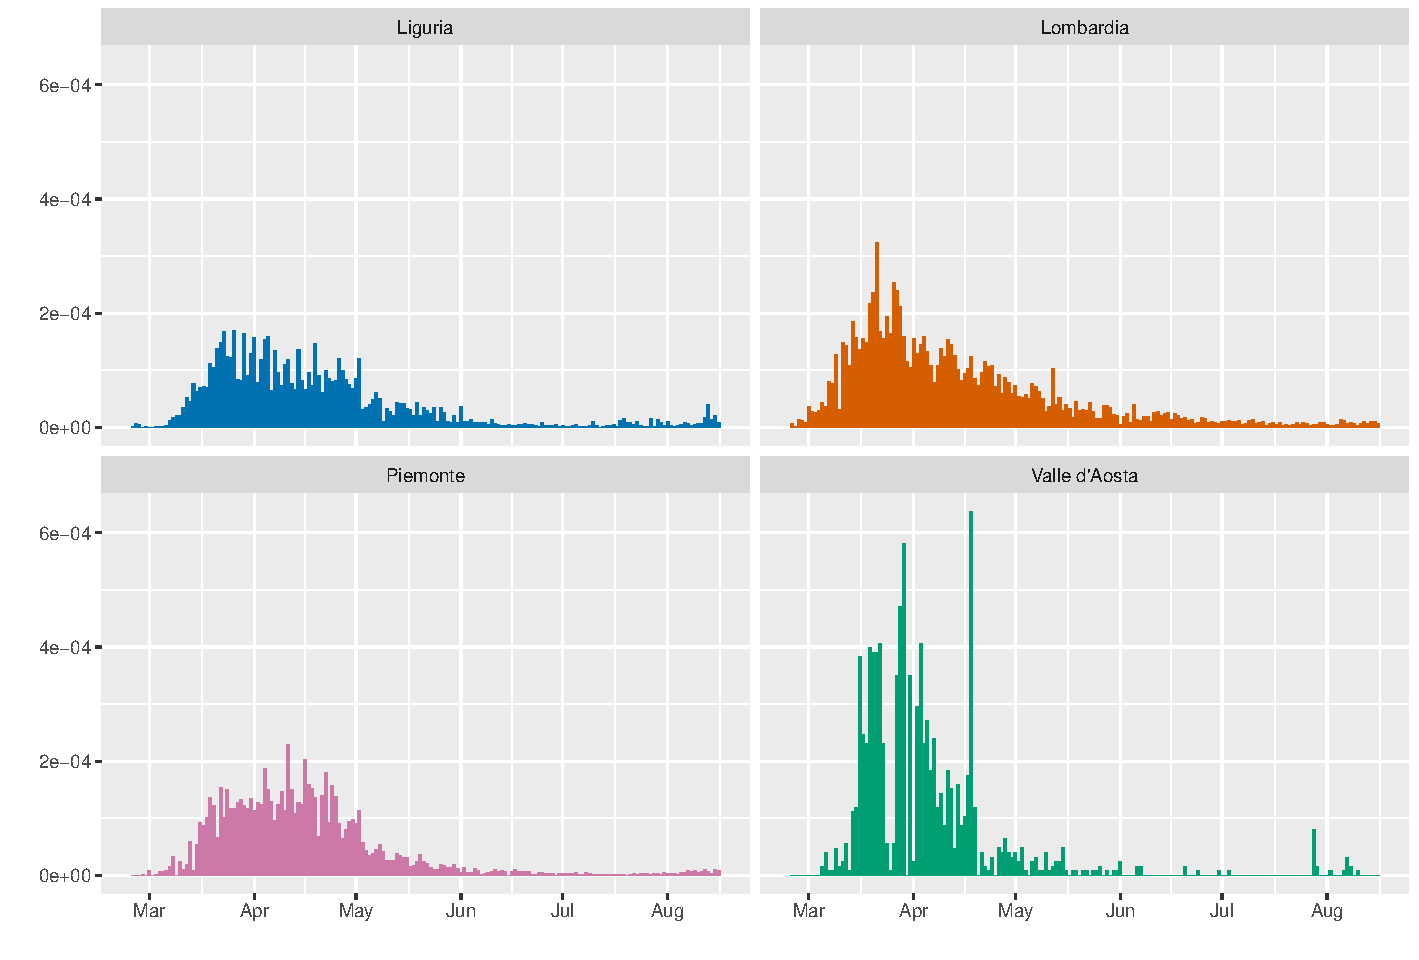
\includegraphics[width=\textwidth]{output/infective_rates_Nord-Ovest.pdf}
    	    \caption{Incidence rate per region for the \textit{Nord-Ovest} (North-West) NUTS 1 region}
    	    \label{fig:incidence_nordovest}
    	\end{figure}
    	
    	\begin{figure}[H]
    	    \centering
    	    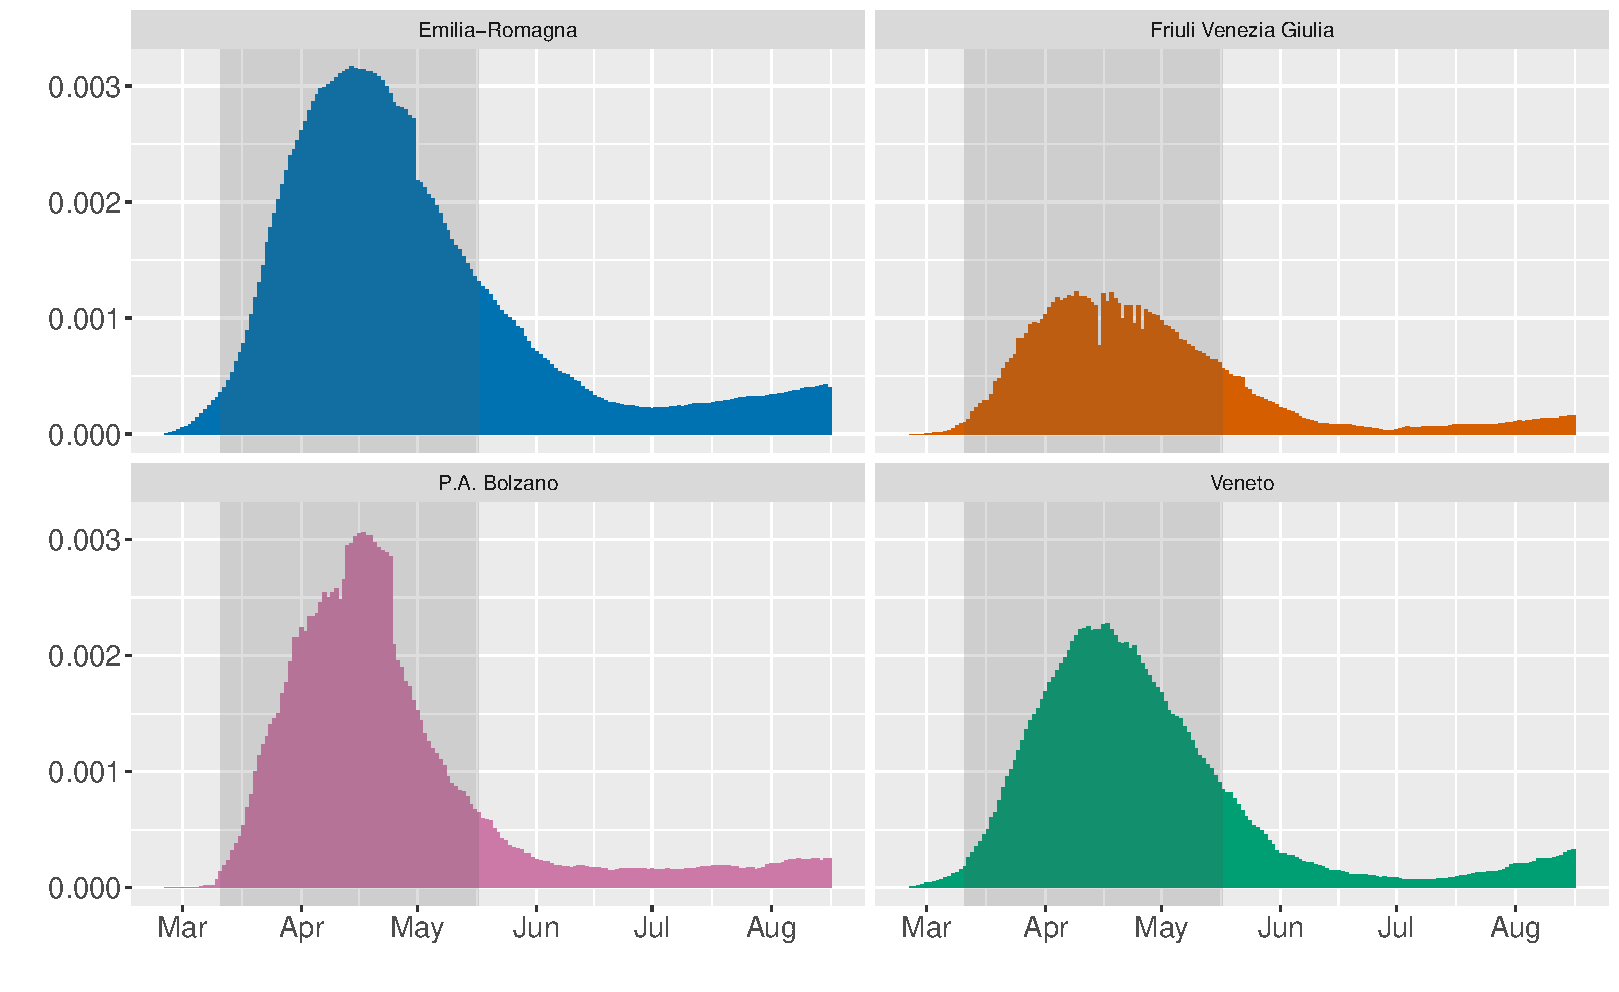
\includegraphics[width=\textwidth]{output/infective_rates_Nord-Est.pdf}
    	    \caption{Incidence rate per region for the \textit{Nord-Est} (North-East) NUTS 1 region}
    	    \label{fig:incidence_nordest}
    	\end{figure}
    	
    	\begin{figure}[H]
    	    \centering
    	    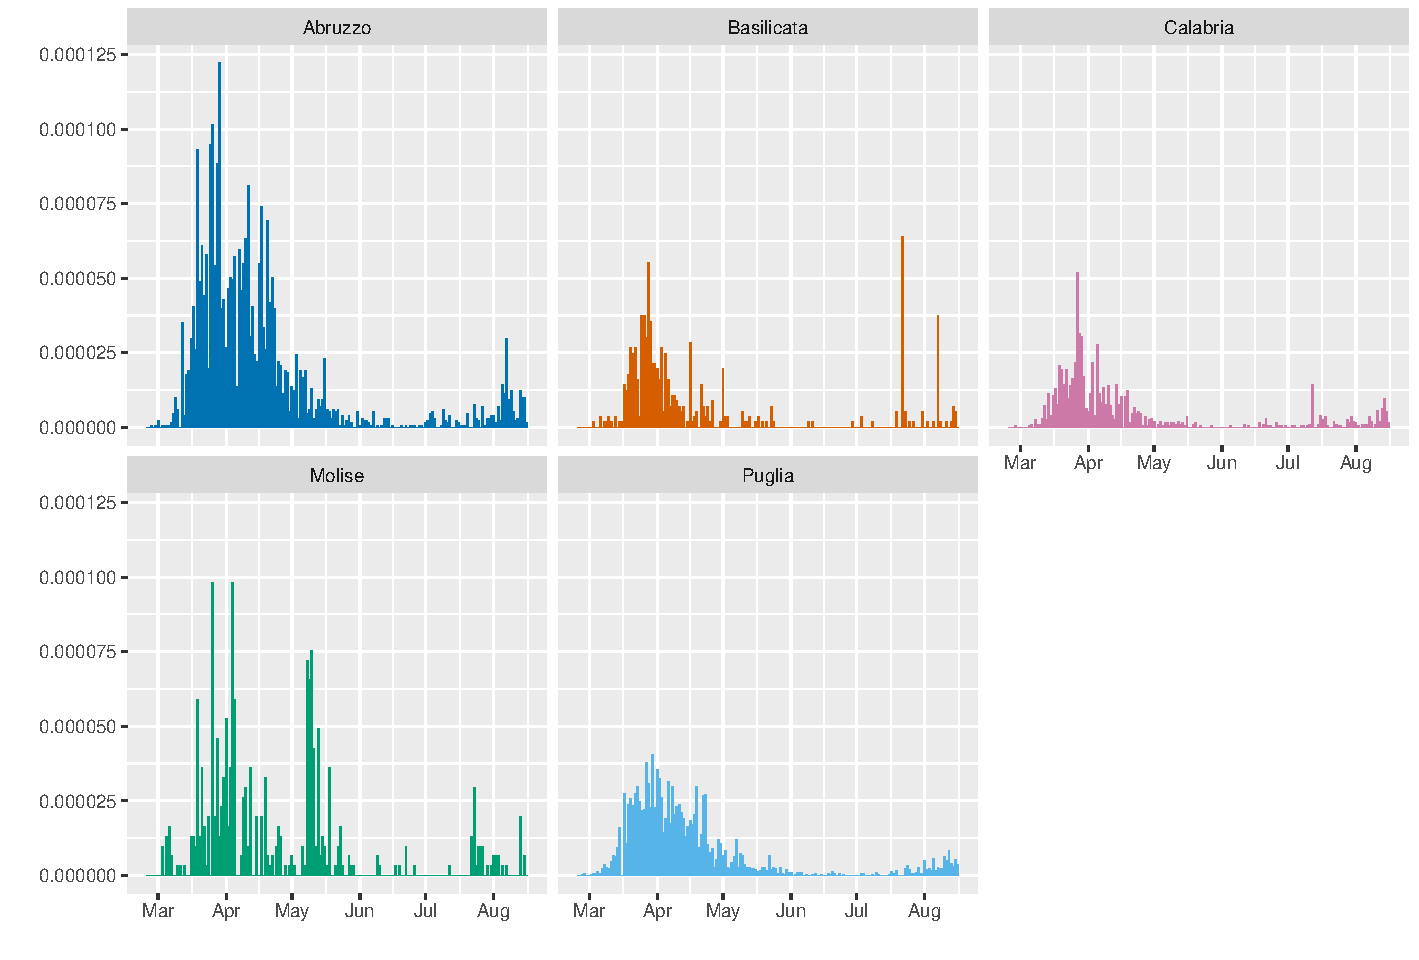
\includegraphics[width=\textwidth]{output/infective_rates_Sud.pdf}
    	    \caption{Incidence rate per region for the \textit{Sud} (South) NUTS 1 region}
    	    \label{fig:incidence_sud}
    	\end{figure}
    	
    	\begin{figure}[H]
    	    \centering
    	    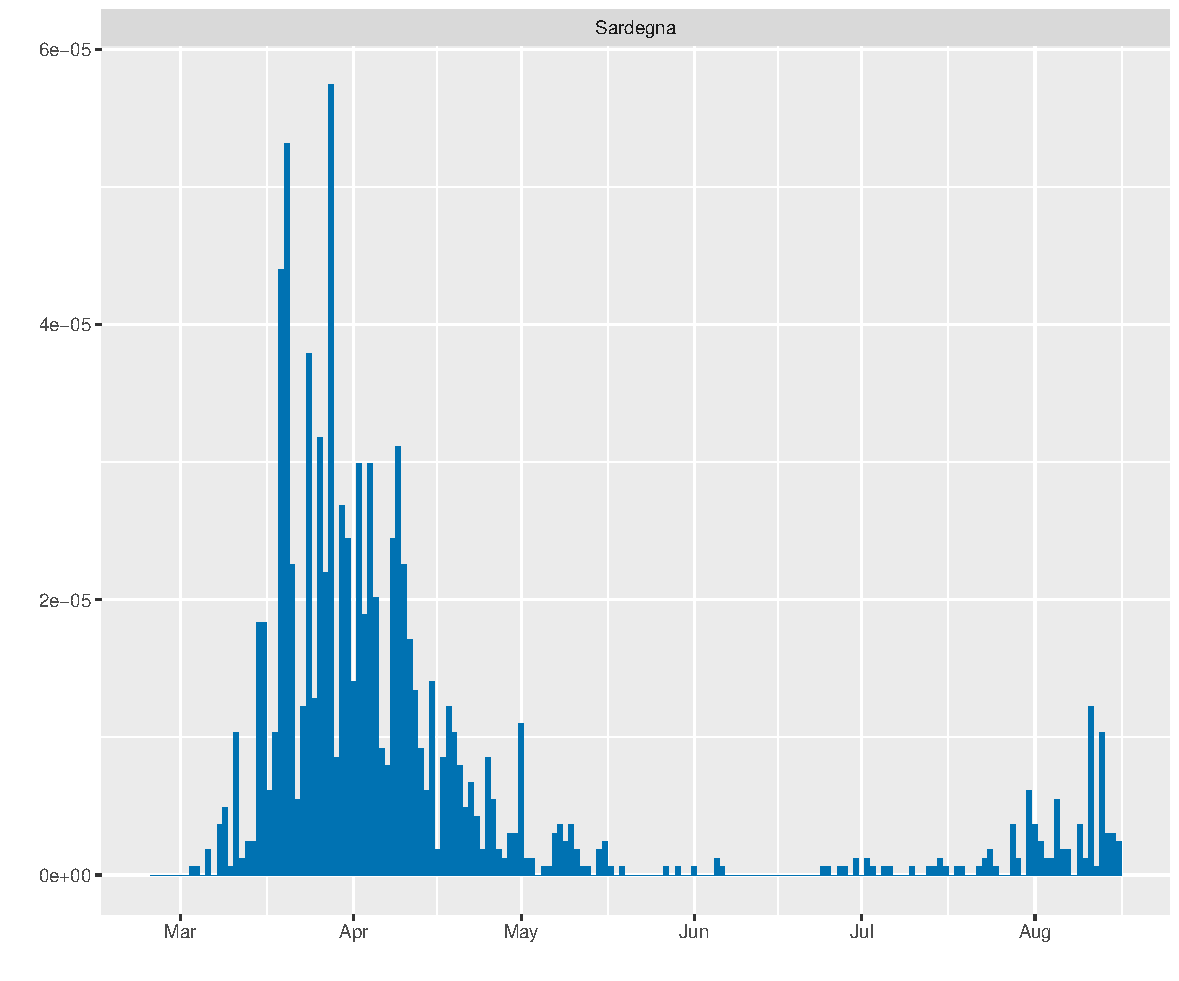
\includegraphics[width=\textwidth]{output/infective_rates_Isole.pdf}
    	    \caption{Incidence rate per region for the \textit{Isole} (Islands) NUTS 1 region}
    	    \label{fig:incidence_isole}
    	\end{figure}
		
		\subsection{Figures for Section \ref{sec:dataset}: \nameref{sec:dataset}} \label{sapp:figures_dataset}
		
		\begin{figure}[H]
    	    \centering
    	    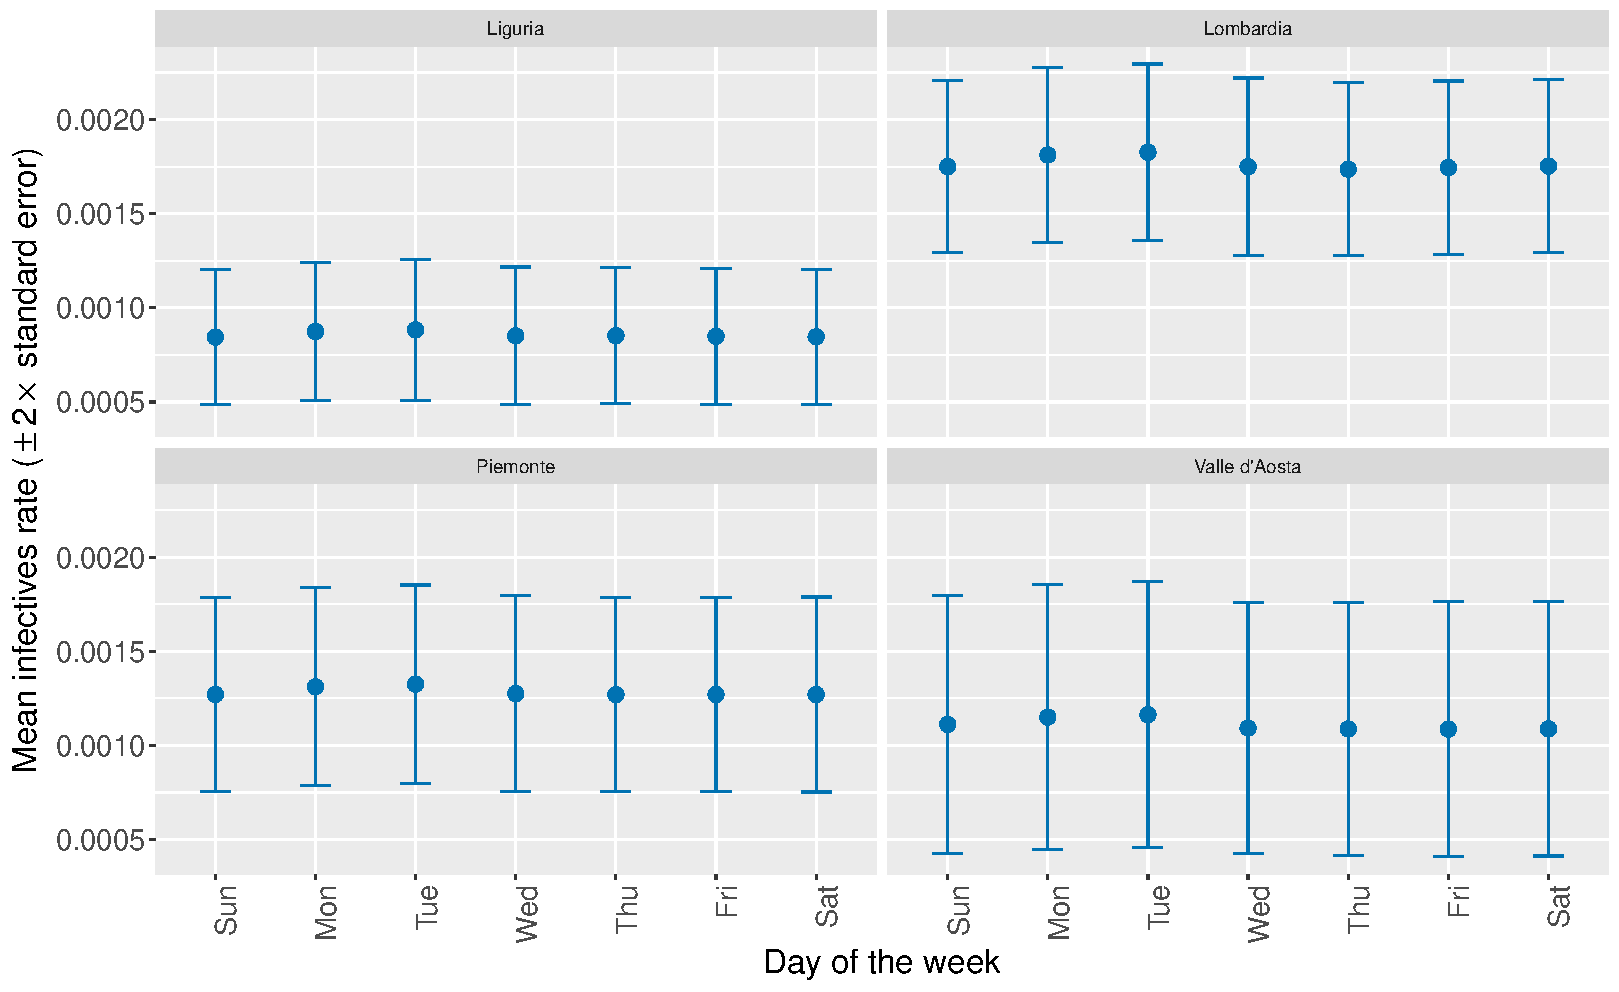
\includegraphics[width=\textwidth]{output/infective_rates_weekday_Nord-Ovest.pdf}
    	    \caption{Incidence rate per NUTS 2 region per day of the week for the \textit{Nord-Ovest} (North-West) NUTS 1 region}
    	    \label{fig:incidence_nordovest_weekday}
    	\end{figure}
		
		\begin{figure}[H]
    	    \centering
    	    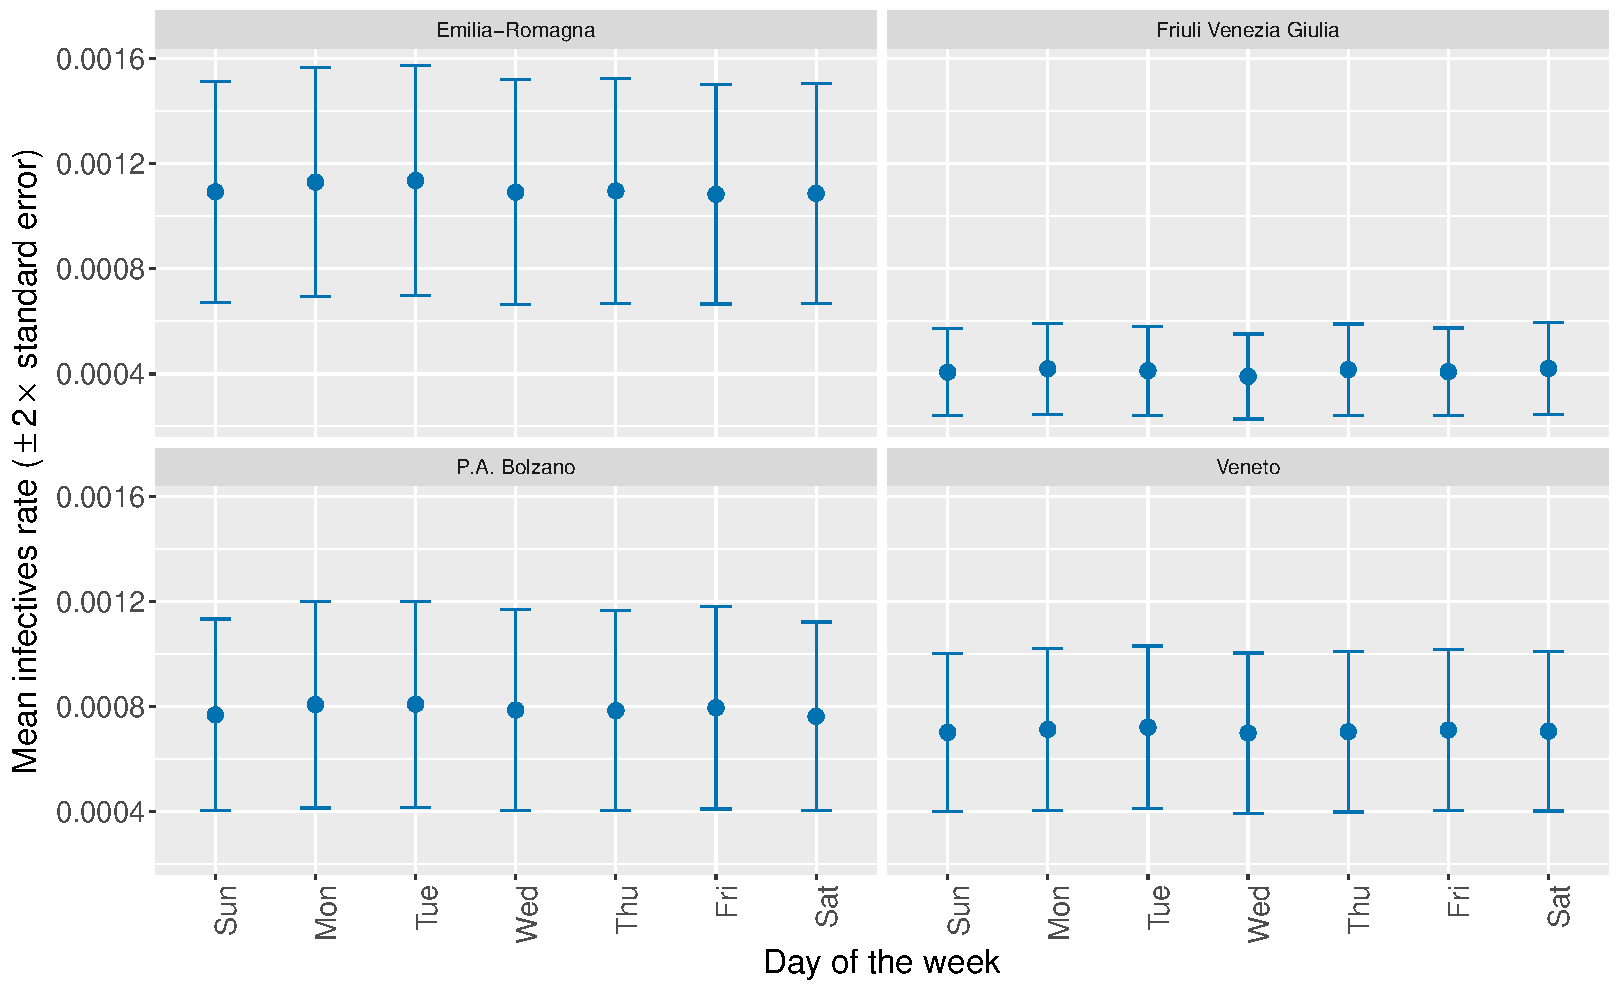
\includegraphics[width=\textwidth]{output/infective_rates_weekday_Nord-Est.pdf}
    	    \caption{Incidence rate per NUTS 2 region per day of the week for the \textit{Nord-Est} (North-East) NUTS 1 region}
    	    \label{fig:incidence_nordest_weekday}
    	\end{figure}
    	
    	\begin{figure}[H]
    	    \centering
    	    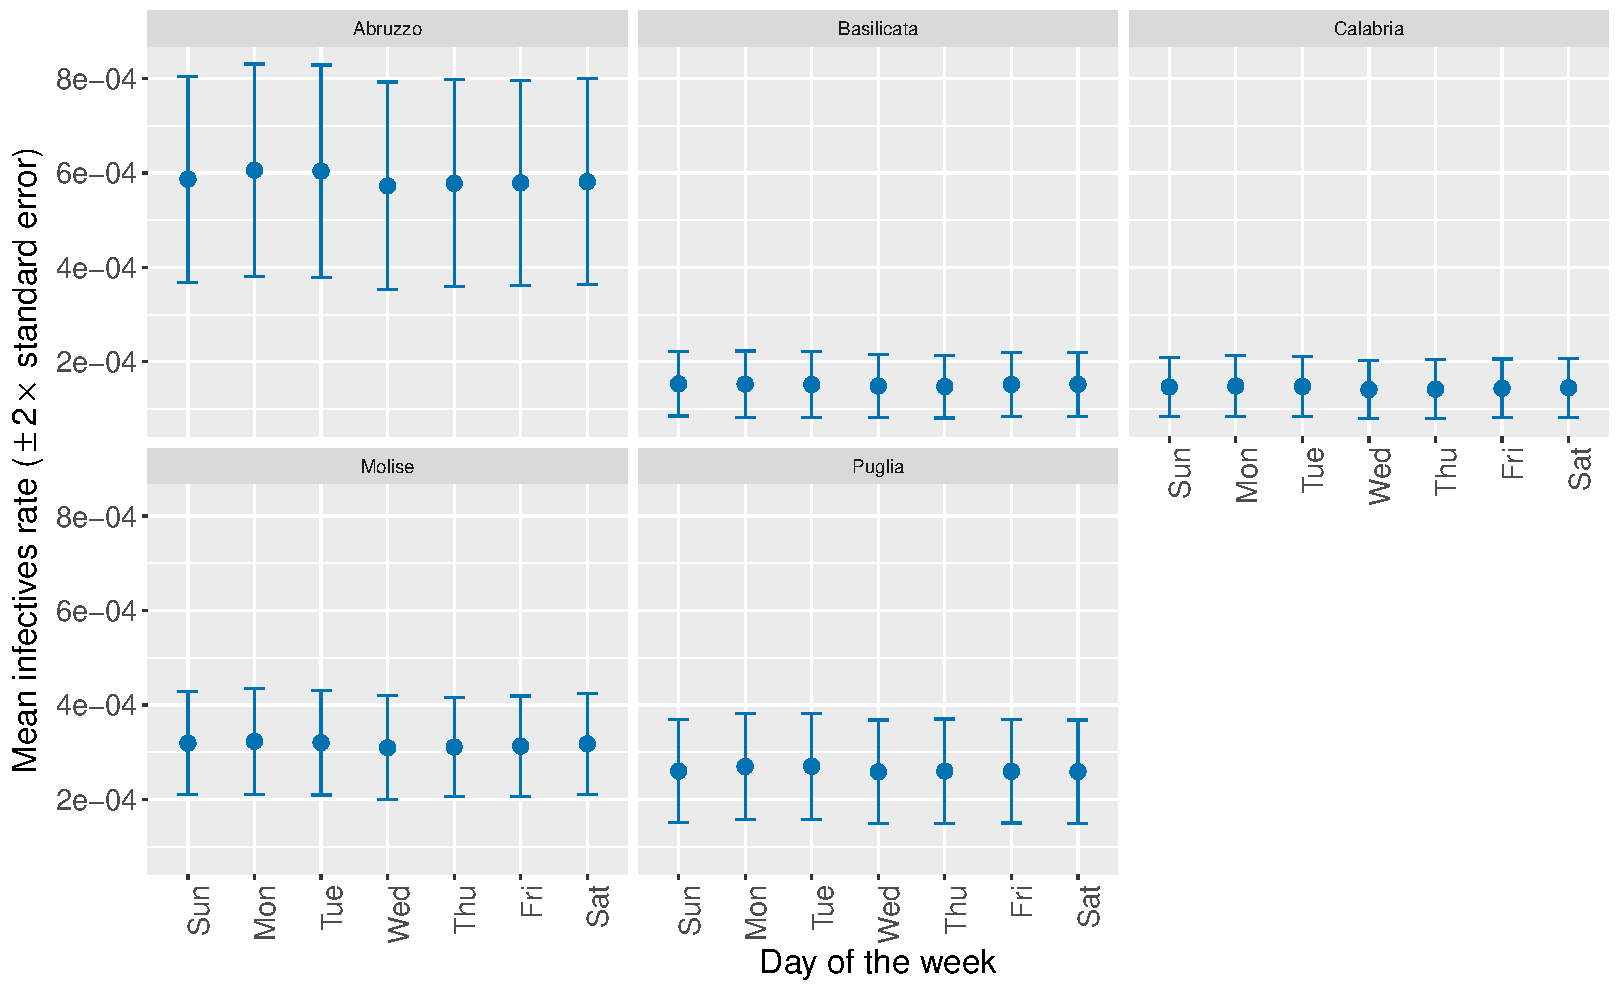
\includegraphics[width=\textwidth]{output/infective_rates_weekday_Sud.pdf}
    	    \caption{Incidence rate per NUTS 2 region per day of the week for the \textit{Sud} (South) NUTS 1 region}
    	    \label{fig:incidence_sud_weekday}
    	\end{figure}
		
		\begin{figure}[H]
    	    \centering
    	    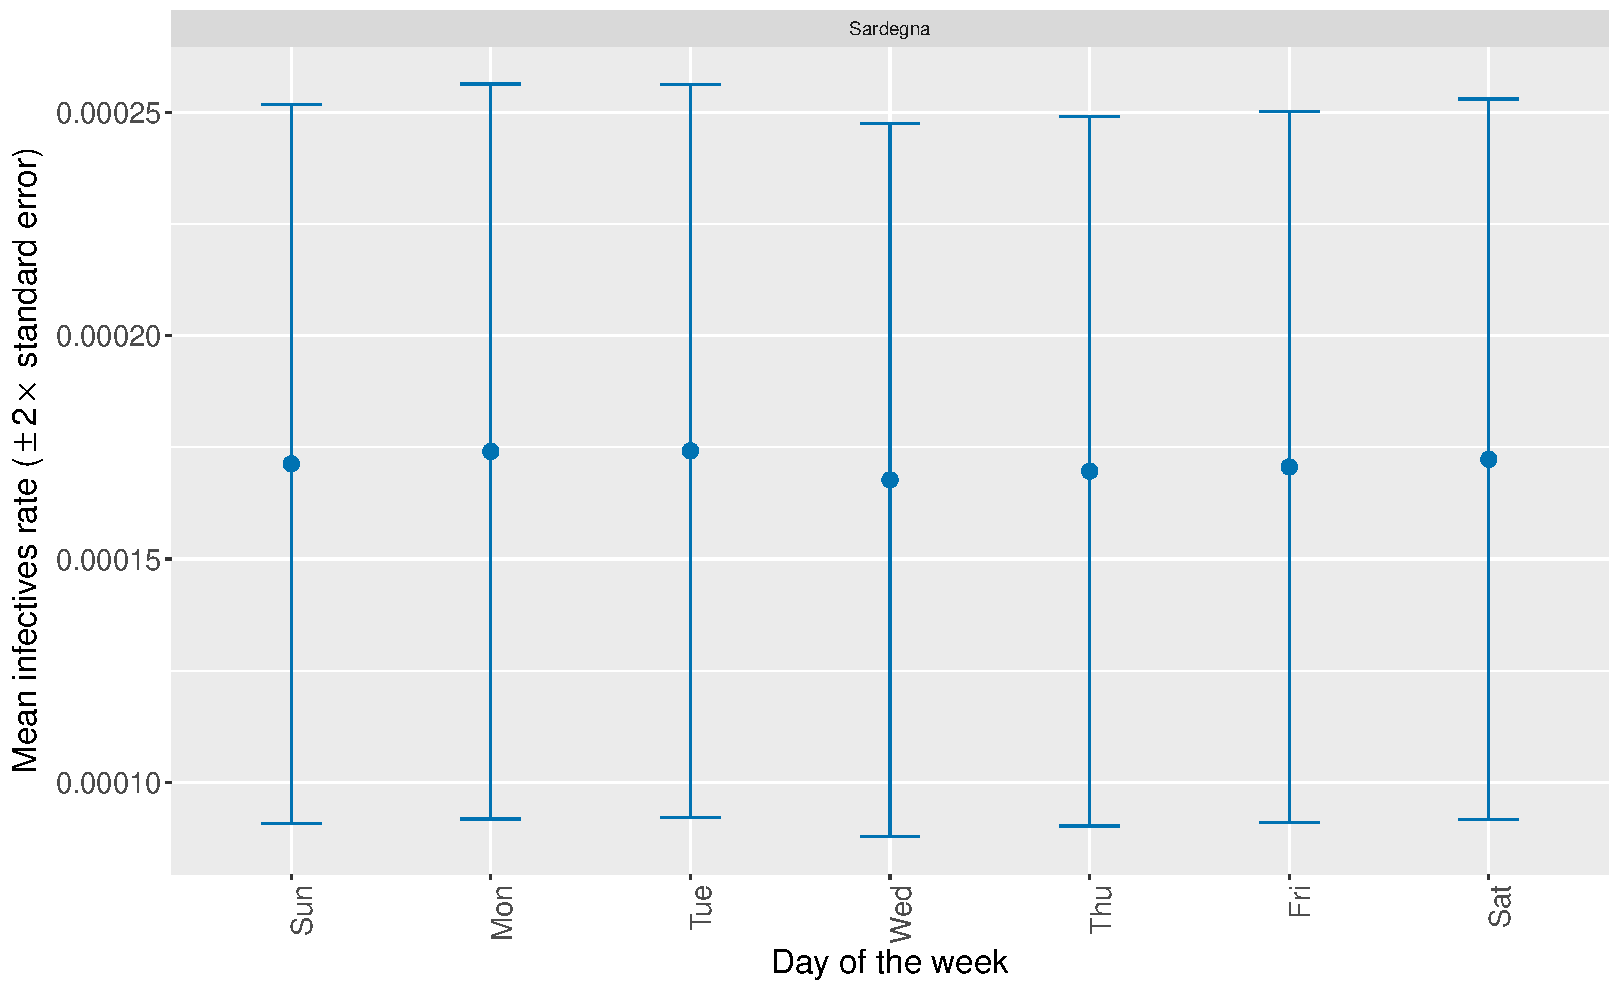
\includegraphics[width=\textwidth]{output/infective_rates_weekday_Isole.pdf}
    	    \caption{Incidence rate per NUTS 2 region per day of the week for the \textit{Isole} (Islands) NUTS 1 region}
    	    \label{fig:incidence_sud_weekday}
    	\end{figure}
		
		\subsection{Plots of $\beta_{within}$ over time} \label{sapp:model1_plots}
		In Section \ref{subsec:results_within} we presented the plots of $\beta_{within}$ over time for the \textit{Nord-Est} (North-East) NUTS 1 region for Within-Region Spread Model. In this section, we present the plots for the other NUTS 1 regions. As is the case for Section \ref{subsec:results_within}, we use the last 100 observations. \\
		
		\begin{figure}[H]
    	    \centering
    	    \begin{subfigure}{\textwidth}
    	      \centering
    	      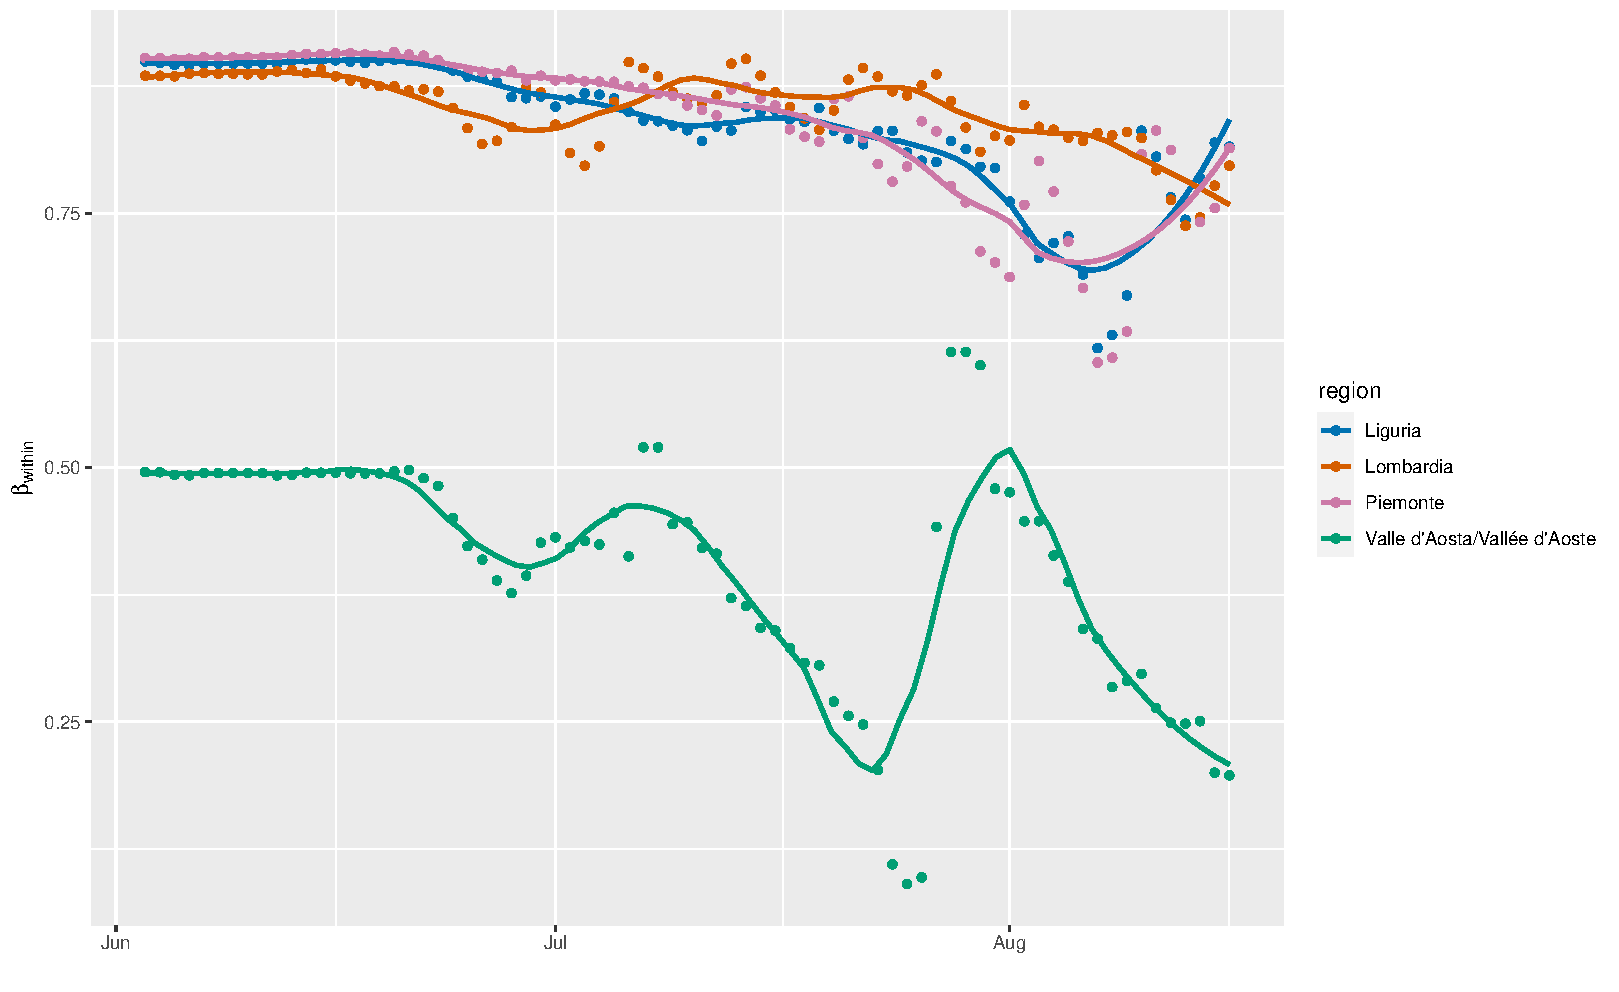
\includegraphics[width=0.95\linewidth]{output/model1_lag3_betawithin_Nord-Ovest_rolling.pdf}
    	      \caption{Without model selection}
    	      \label{fig:beta_within_over_time_northwest_regular}
    	    \end{subfigure}\newline
    	    \begin{subfigure}{\textwidth}
    	      \centering
    	      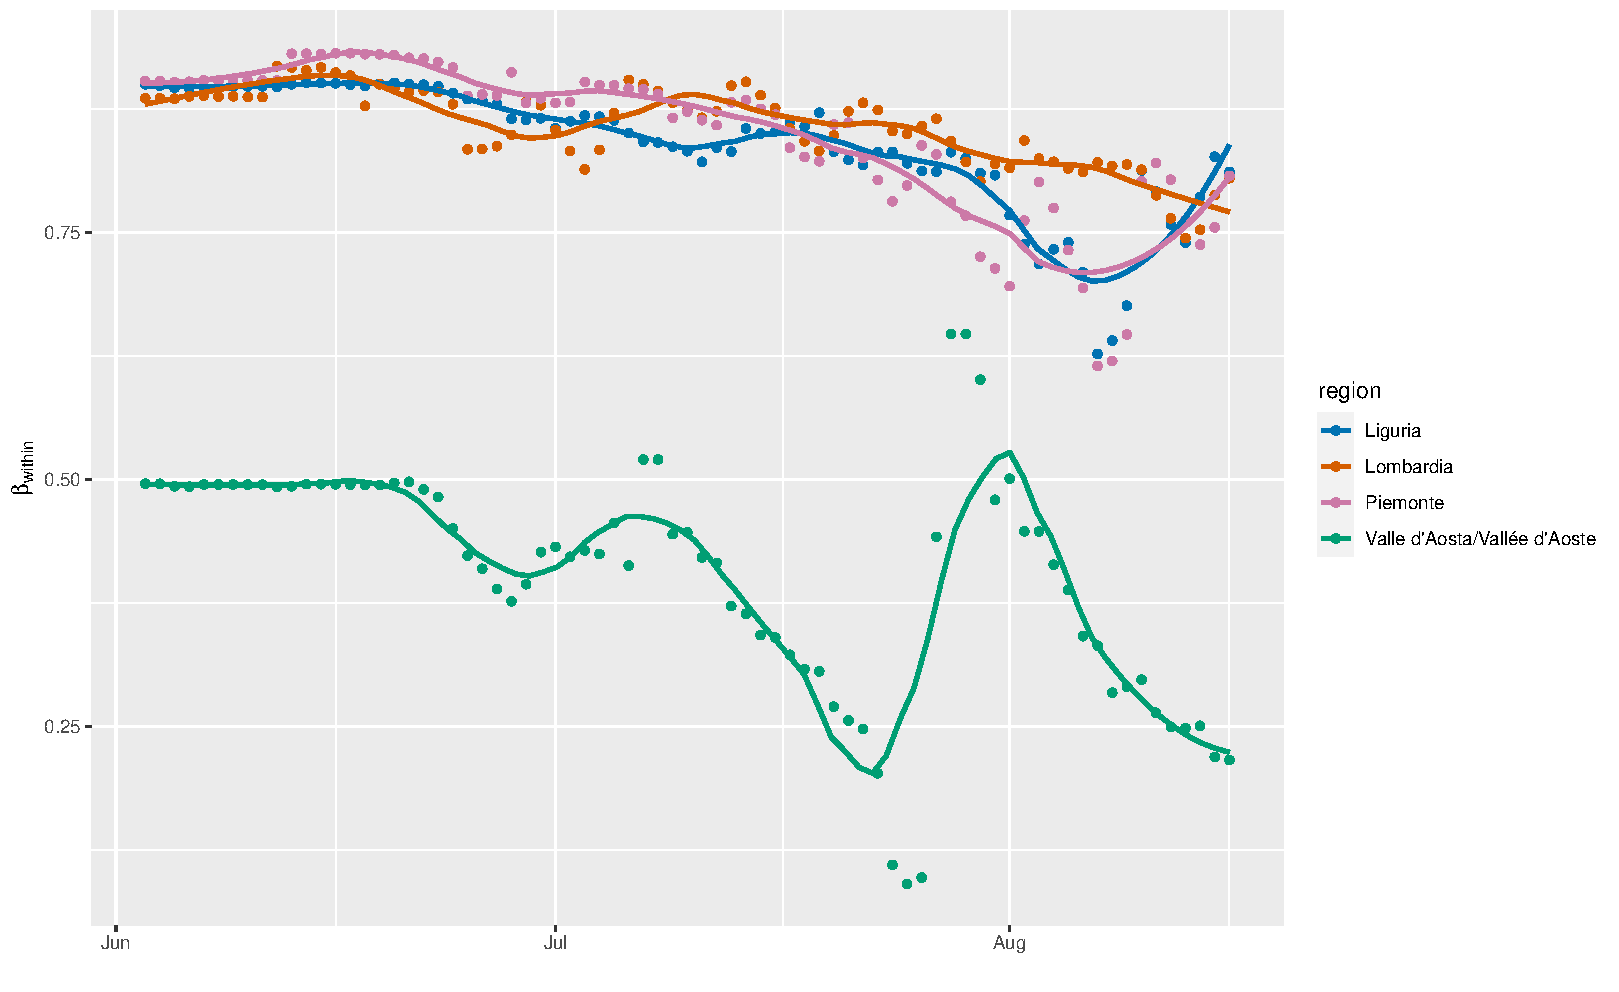
\includegraphics[width=0.95\linewidth]{output/model1_lag3_betawithin_Nord-Ovest_aic_rolling.pdf}
    	      \caption{With model selection by AIC}
    	      \label{fig:beta_within_over_time_northwest_aic}
    	    \end{subfigure}
        \end{figure}
        \begin{figure}[H]\ContinuedFloat
    	    \begin{subfigure}{\textwidth}
    	      \centering
    	      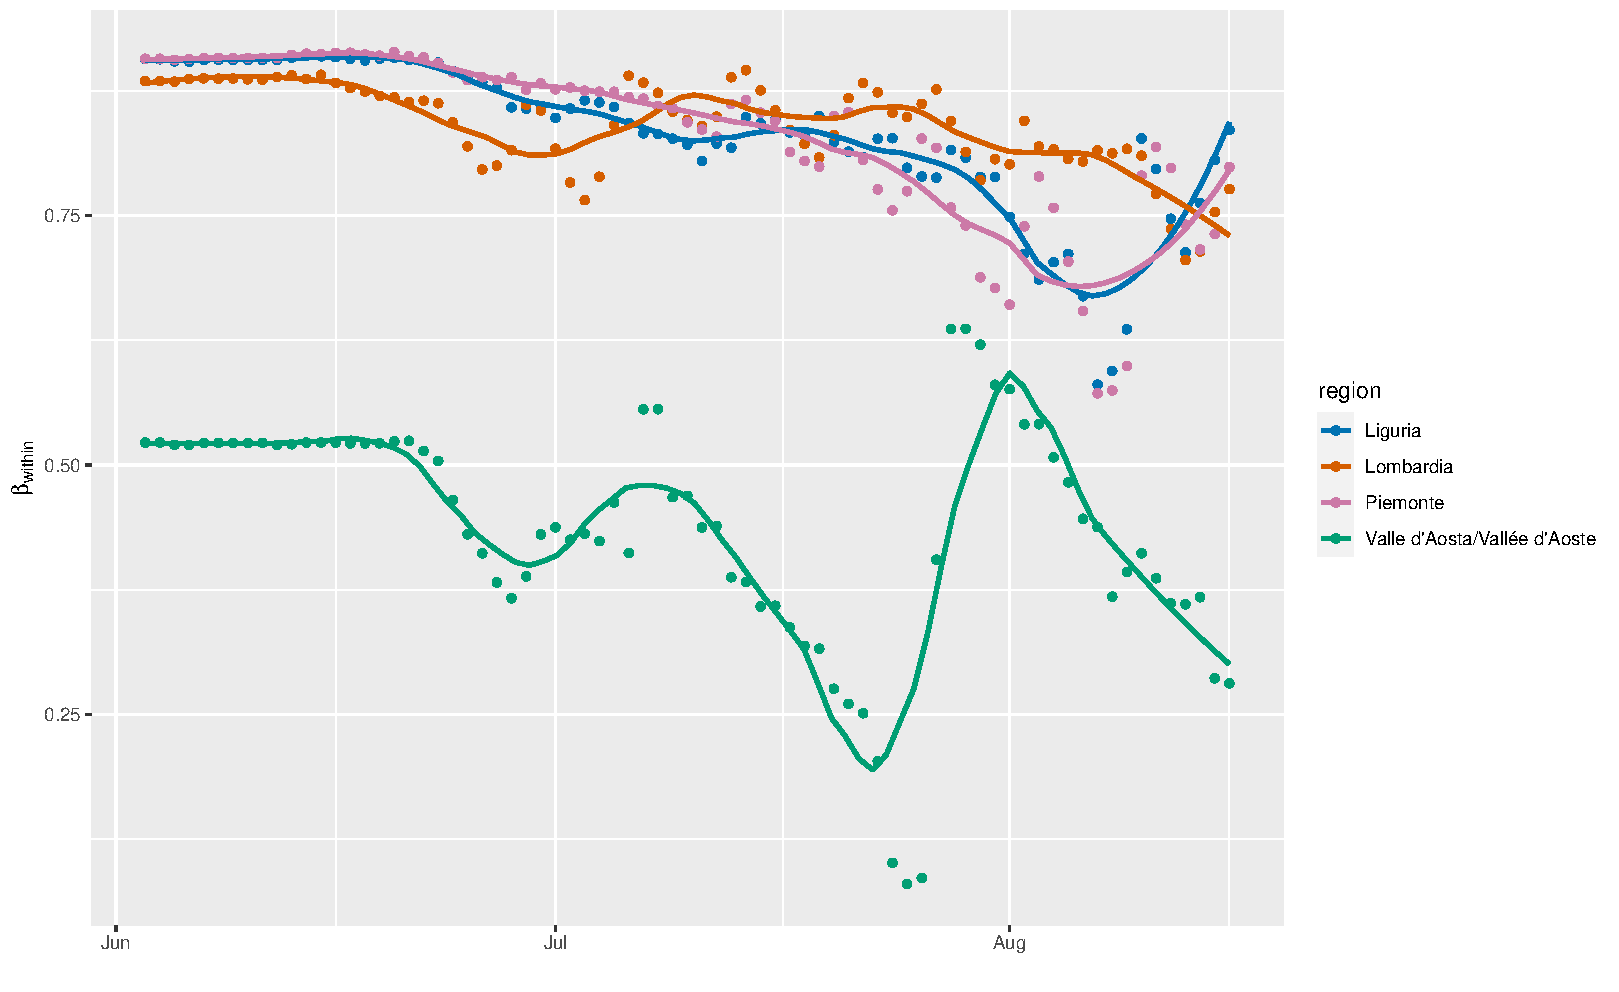
\includegraphics[width=0.95\linewidth]{output/model1_lag3_betawithin_Nord-Ovest_UndocQuadratic_rolling.pdf}
    	      \caption{Without model selection; \\ including undocumented infectives}
    	      \label{fig:beta_within_over_time_northwest_regular_undoc}
    	    \end{subfigure}\newline
    	    \begin{subfigure}{\textwidth}
    	      \centering
    	      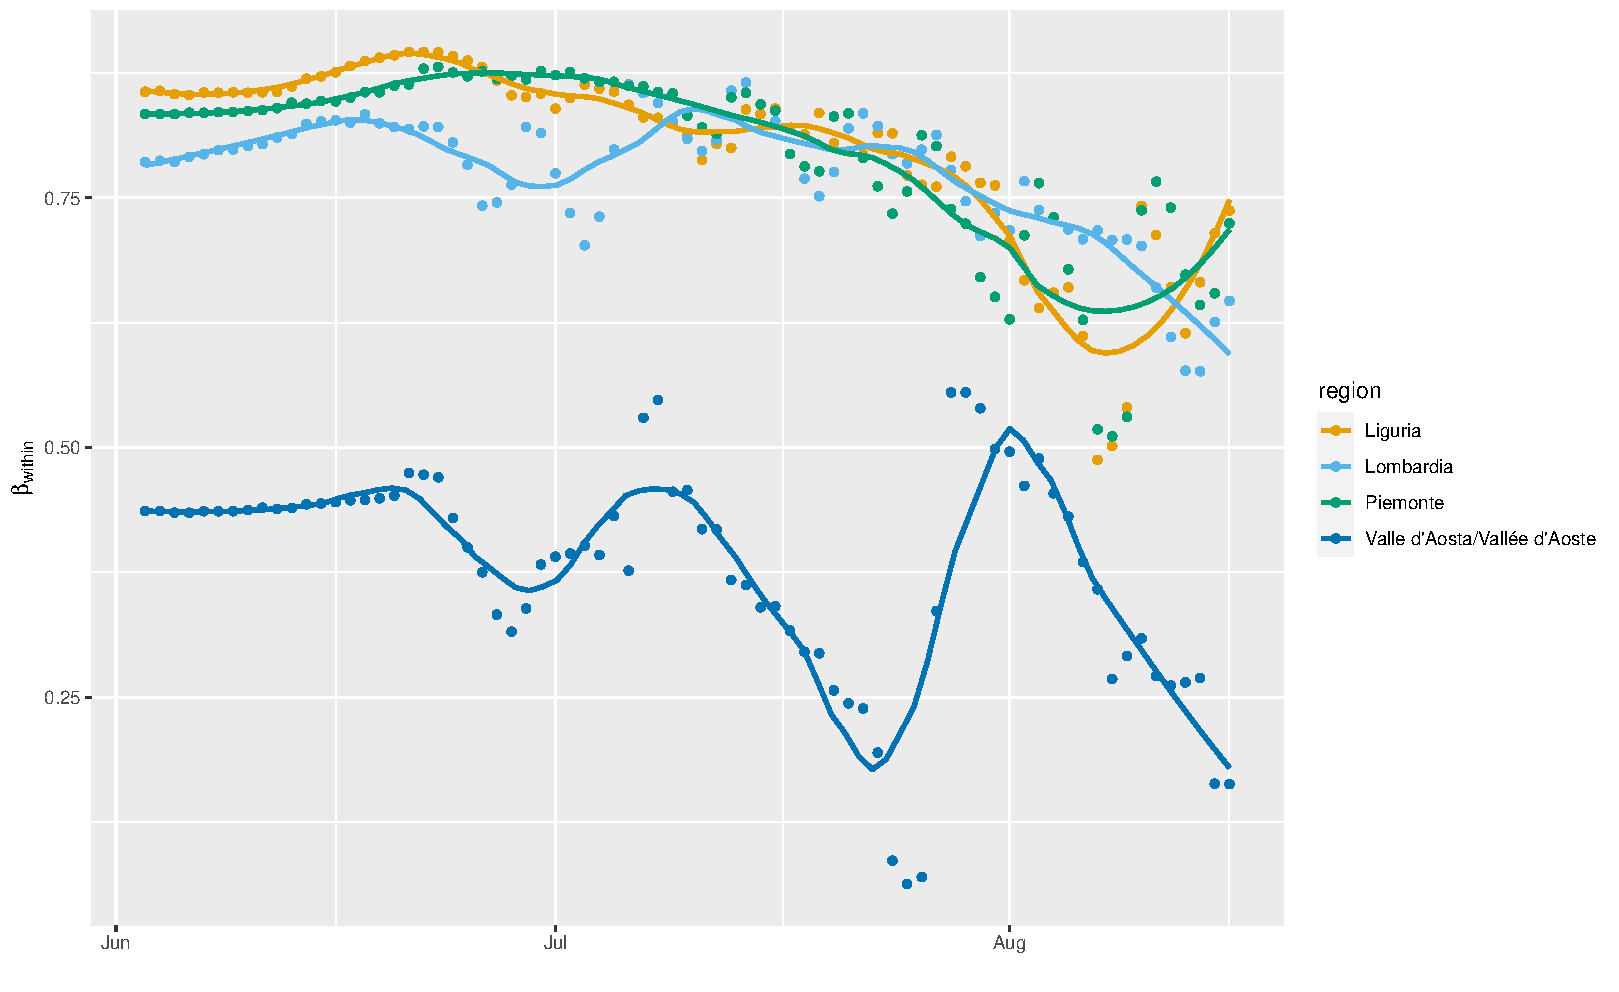
\includegraphics[width=0.95\linewidth]{output/model1_lag3_betawithin_Nord-Ovest_aic_UndocQuadratic_rolling.pdf}
    	      \caption{With model selection by AIC; \\ including undocumented infectives}
    	      \label{fig:beta_within_over_time_northwest_aic_undoc}
    	    \end{subfigure}
    	    \caption{Progression of $\beta_{within}$ over time for the \textit{Nord-Ovest} (North-West) NUTS 1 region}
    	    \label{fig:beta_within_over_time_northwest}
    	\end{figure}
		
		\begin{figure}[H]
    	    \centering
    	    \begin{subfigure}{\textwidth}
    	      \centering
    	      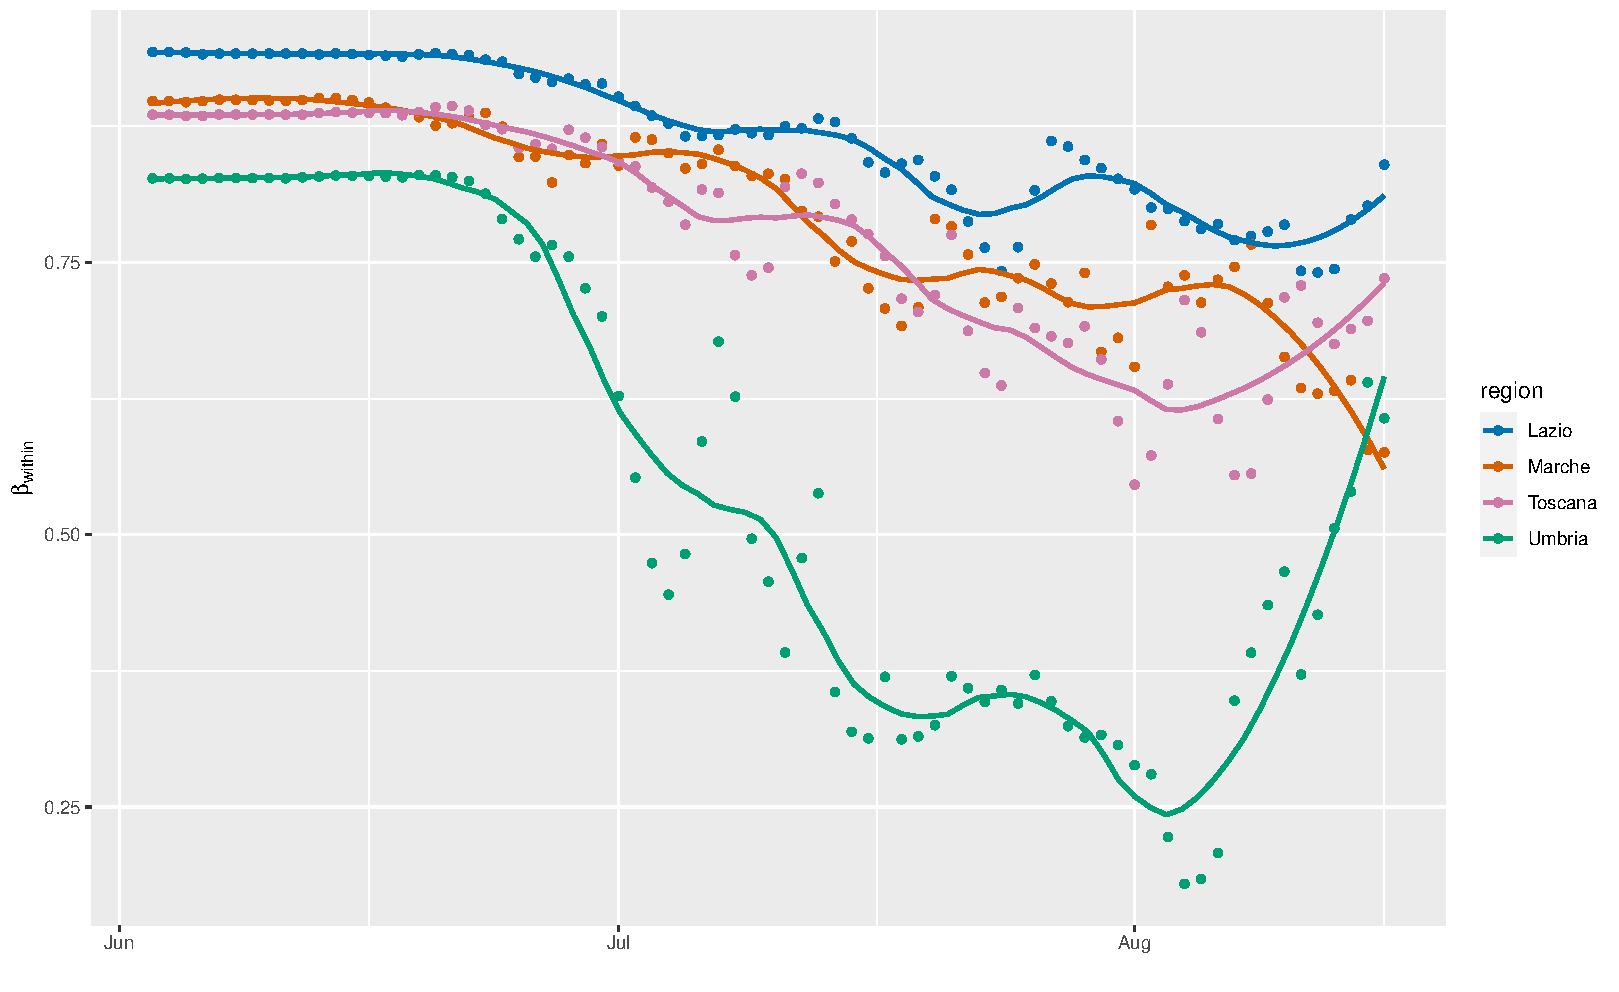
\includegraphics[width=0.95\linewidth]{output/model1_lag3_betawithin_Centro (IT)_rolling.pdf}
    	      \caption{Without model selection}
    	      \label{fig:beta_within_over_time_centro_regular}
    	    \end{subfigure}\newline
    	    \begin{subfigure}{\textwidth}
    	      \centering
    	      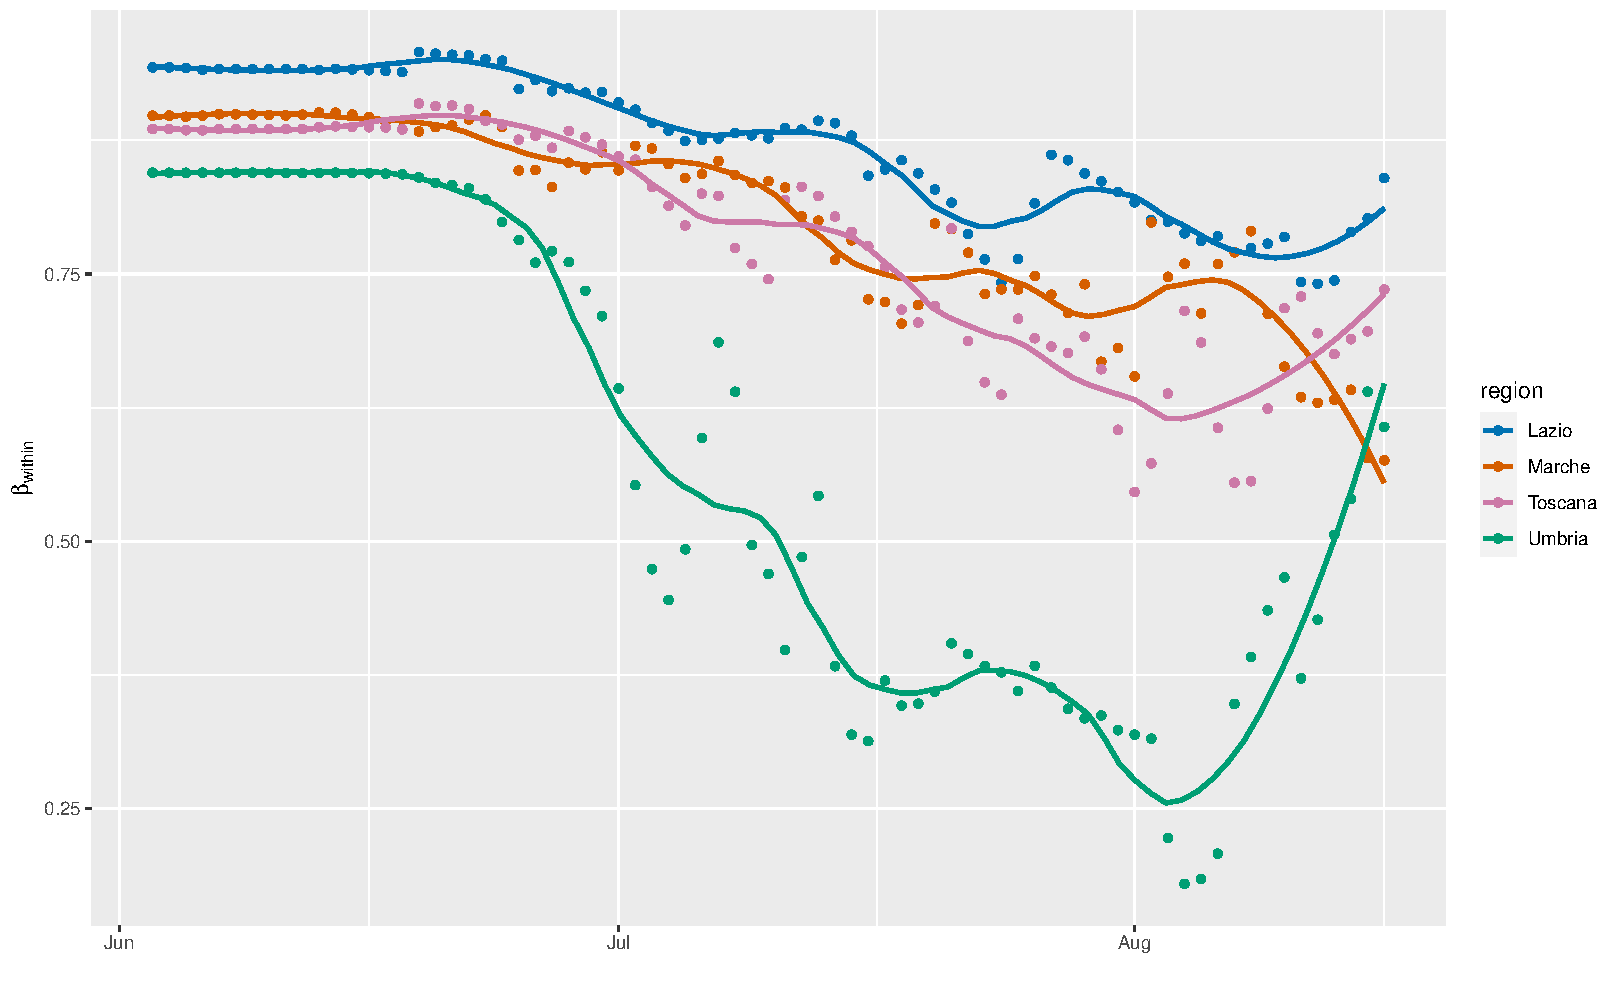
\includegraphics[width=0.95\linewidth]{output/model1_lag3_betawithin_Centro (IT)_aic_rolling.pdf}
    	      \caption{With model selection by AIC}
    	      \label{fig:beta_within_over_time_centro_aic}
    	    \end{subfigure}
    	\end{figure}
        \begin{figure}[H]\ContinuedFloat
    	    \begin{subfigure}{\textwidth}
    	      \centering
    	      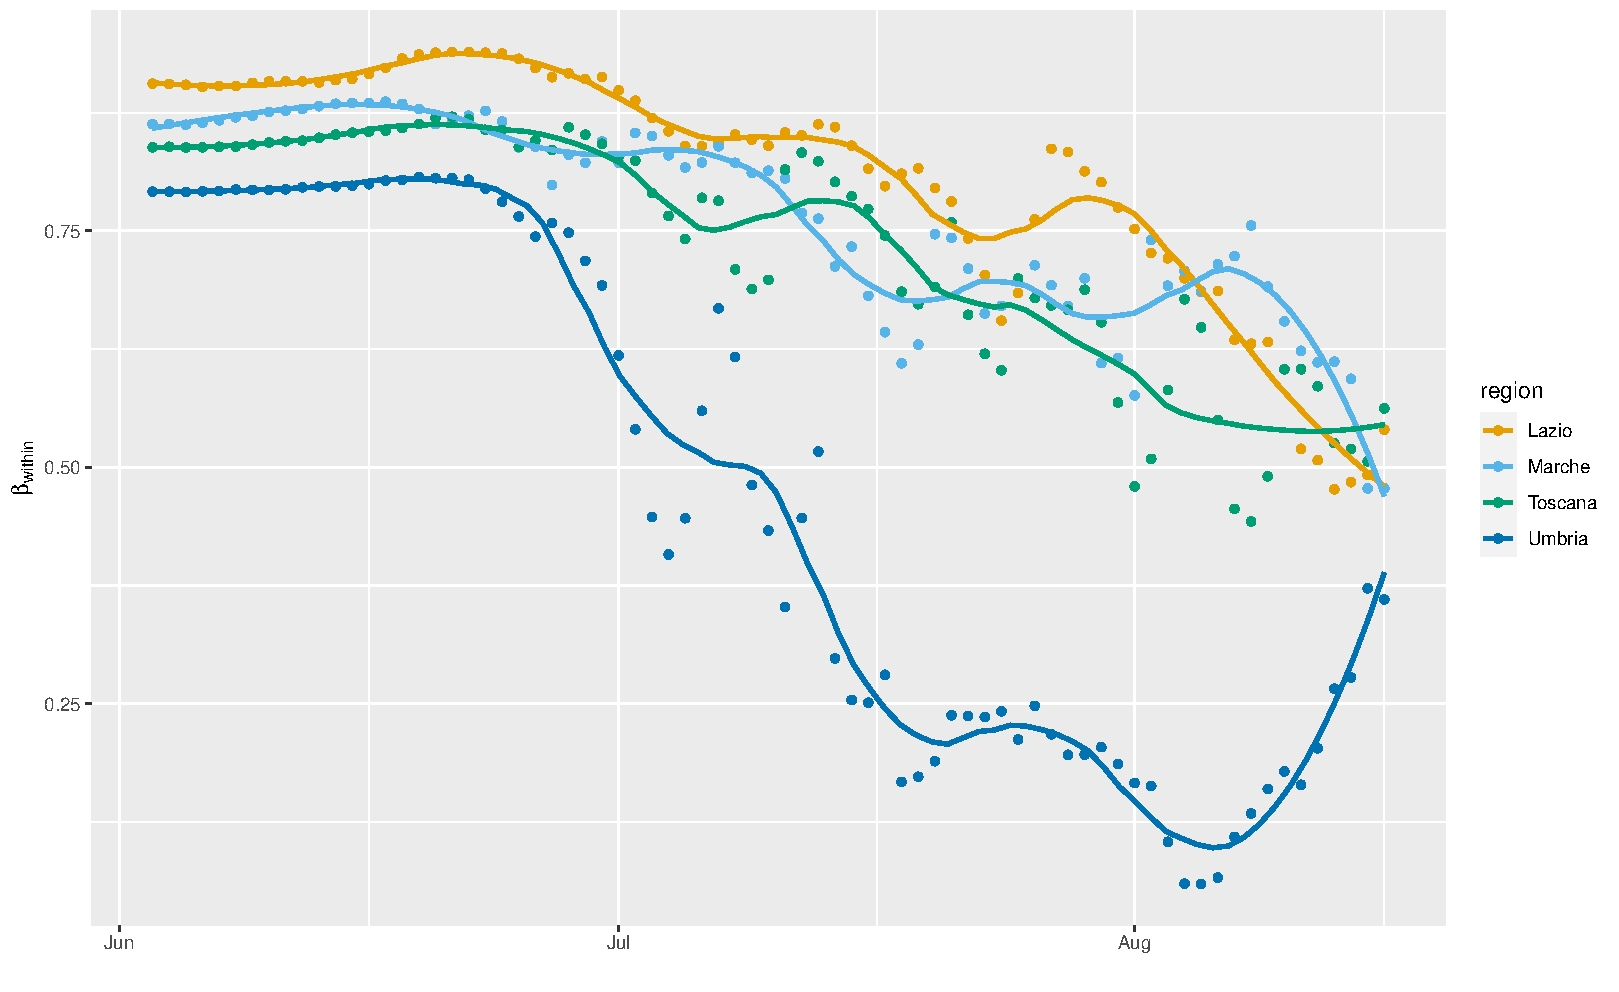
\includegraphics[width=0.95\linewidth]{output/model1_lag3_betawithin_Centro (IT)_UndocQuadratic_rolling.pdf}
    	      \caption{Without model selection; \\ including undocumented infectives}
    	      \label{fig:beta_within_over_time_centro_regular_undoc}
    	    \end{subfigure}\newline
    	    \begin{subfigure}{\textwidth}
    	      \centering
    	      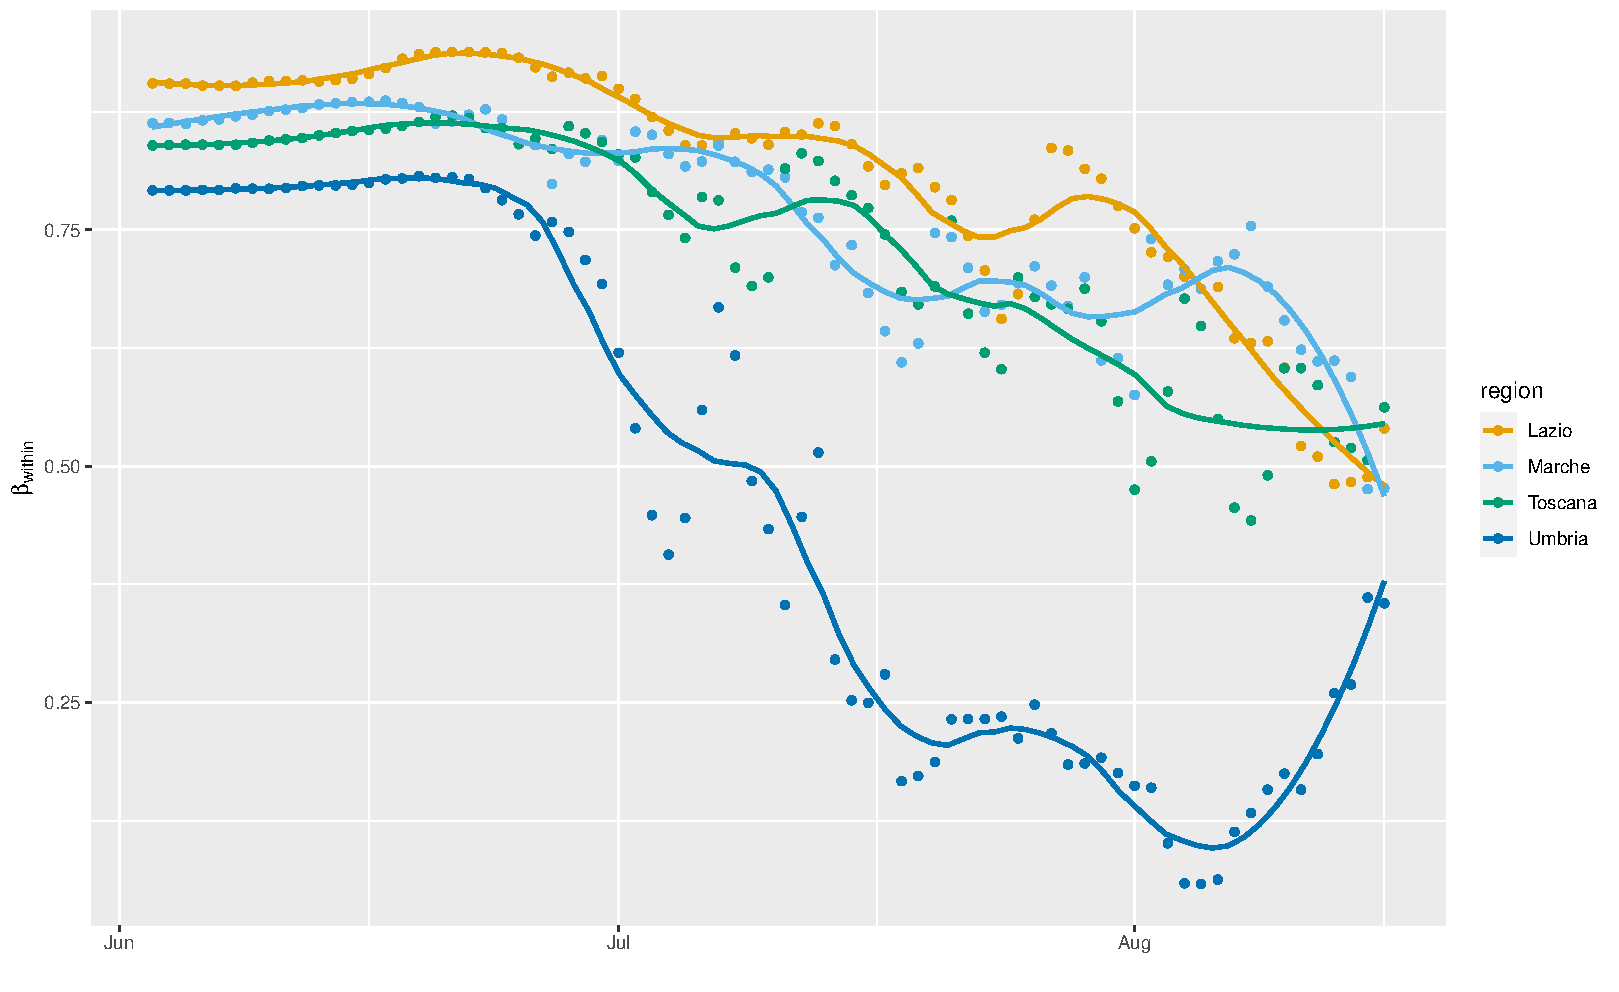
\includegraphics[width=0.95\linewidth]{output/model1_lag3_betawithin_Centro (IT)_aic_UndocQuadratic_rolling.pdf}
    	      \caption{With model selection by AIC; \\ including undocumented infectives}
    	      \label{fig:beta_within_over_time_centro_aic_undoc}
    	    \end{subfigure}
    	    \caption{Progression of $\beta_{within}$ over time for the \textit{Centro (IT)} (Centre) NUTS 1 region}
    	    \label{fig:beta_within_over_time_centro}
	    \end{figure}
		
		\begin{figure}[H]
    	    \centering
    	    \begin{subfigure}{\textwidth}
    	      \centering
    	      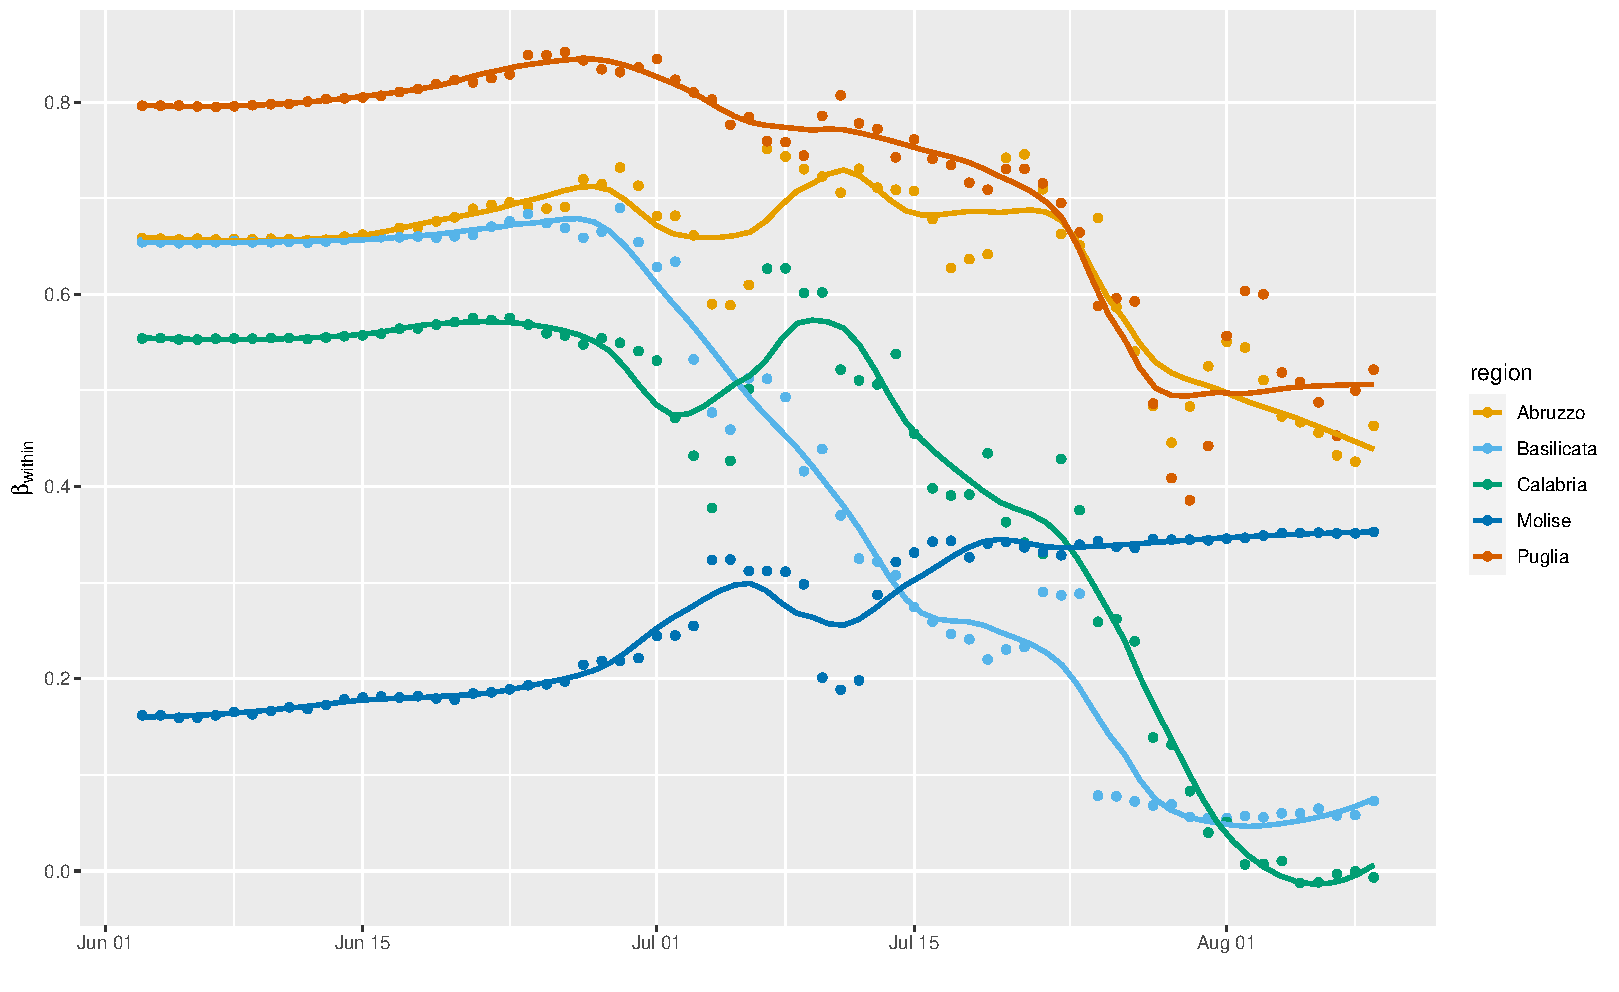
\includegraphics[width=0.95\linewidth]{output/model1_lag3_betawithin_Sud_rolling.pdf}
    	      \caption{Without model selection}
    	      \label{fig:beta_within_over_time_sud_regular}
    	    \end{subfigure}\newline
    	    \begin{subfigure}{\textwidth}
    	      \centering
    	      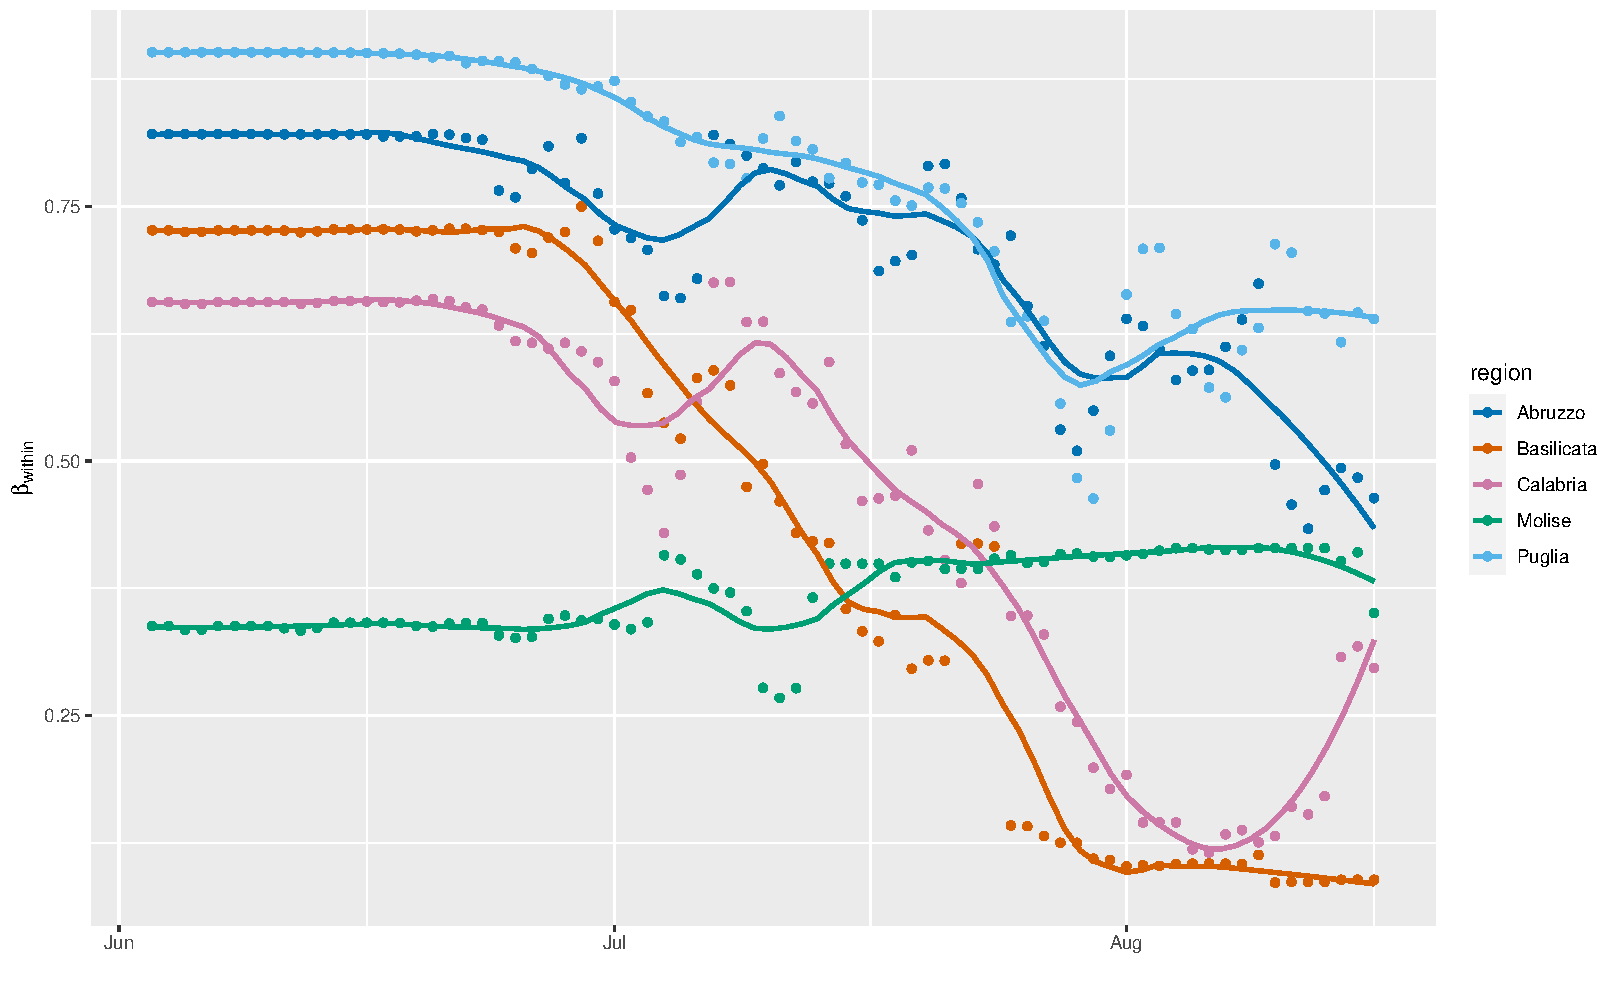
\includegraphics[width=0.95\linewidth]{output/model1_lag3_betawithin_Sud_aic_rolling.pdf}
    	      \caption{With model selection by AIC}
    	      \label{fig:beta_within_over_time_sud_aic}
    	    \end{subfigure}
    	\end{figure}
        \begin{figure}[H]\ContinuedFloat
    	    \begin{subfigure}{\textwidth}
    	      \centering
    	      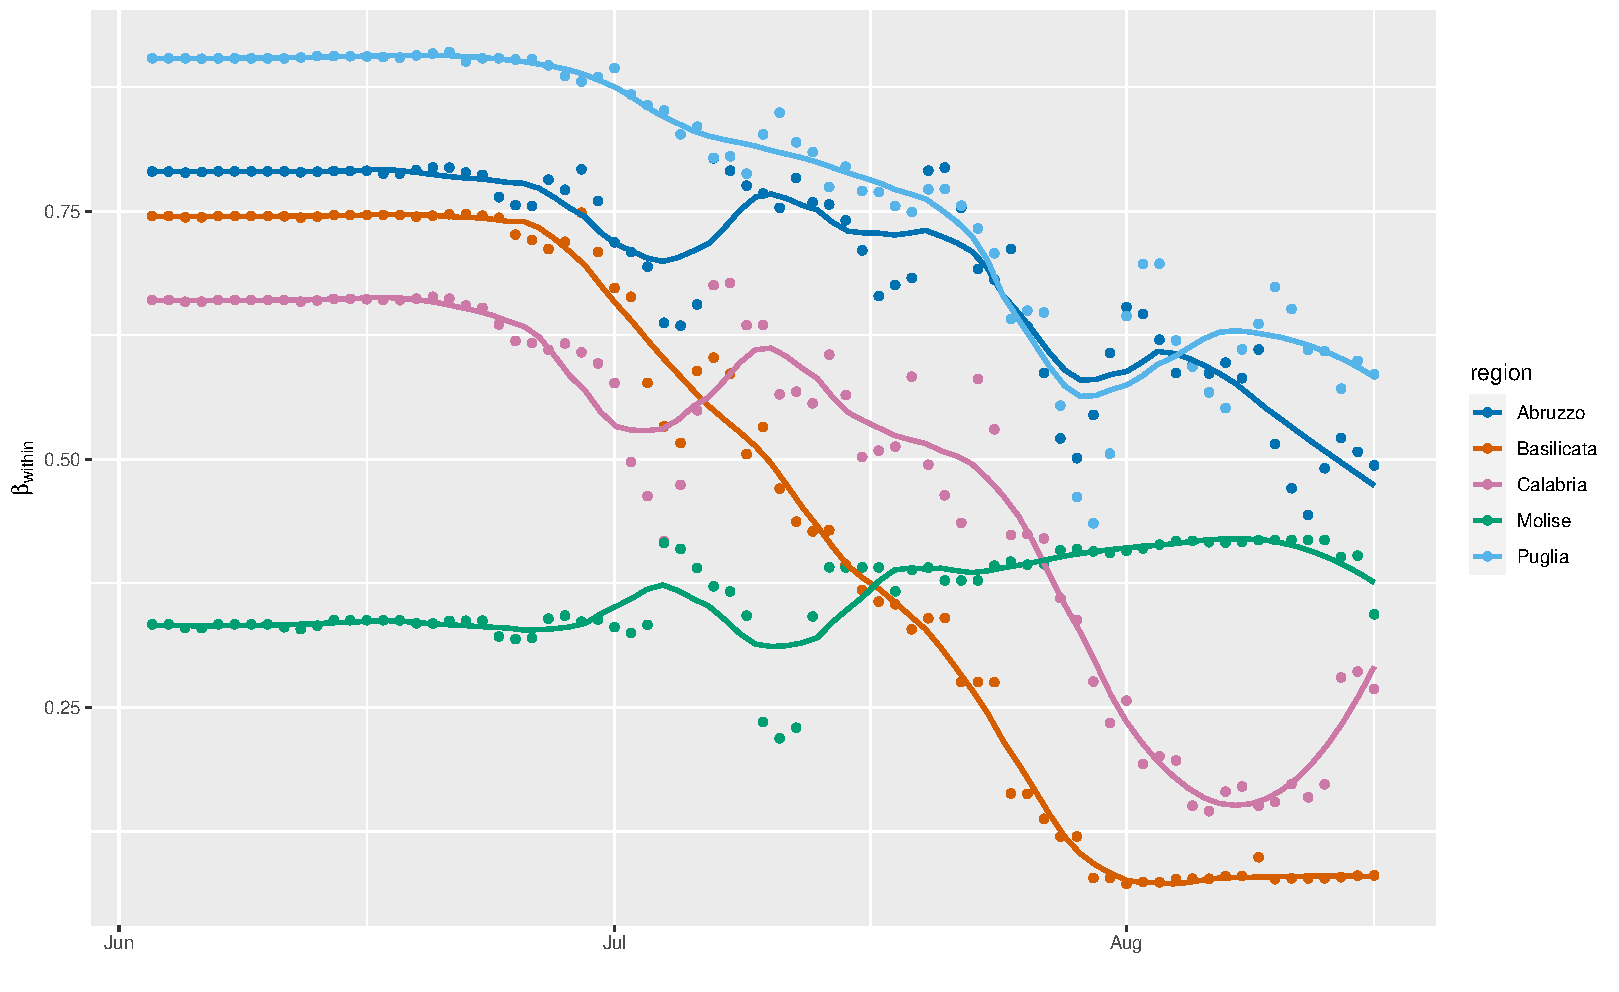
\includegraphics[width=0.95\linewidth]{output/model1_lag3_betawithin_Sud_UndocQuadratic_rolling.pdf}
    	      \caption{Without model selection; \\ including undocumented infectives}
    	      \label{fig:beta_within_over_time_sud_regular_undoc}
    	    \end{subfigure}\newline
    	    \begin{subfigure}{\textwidth}
    	      \centering
    	      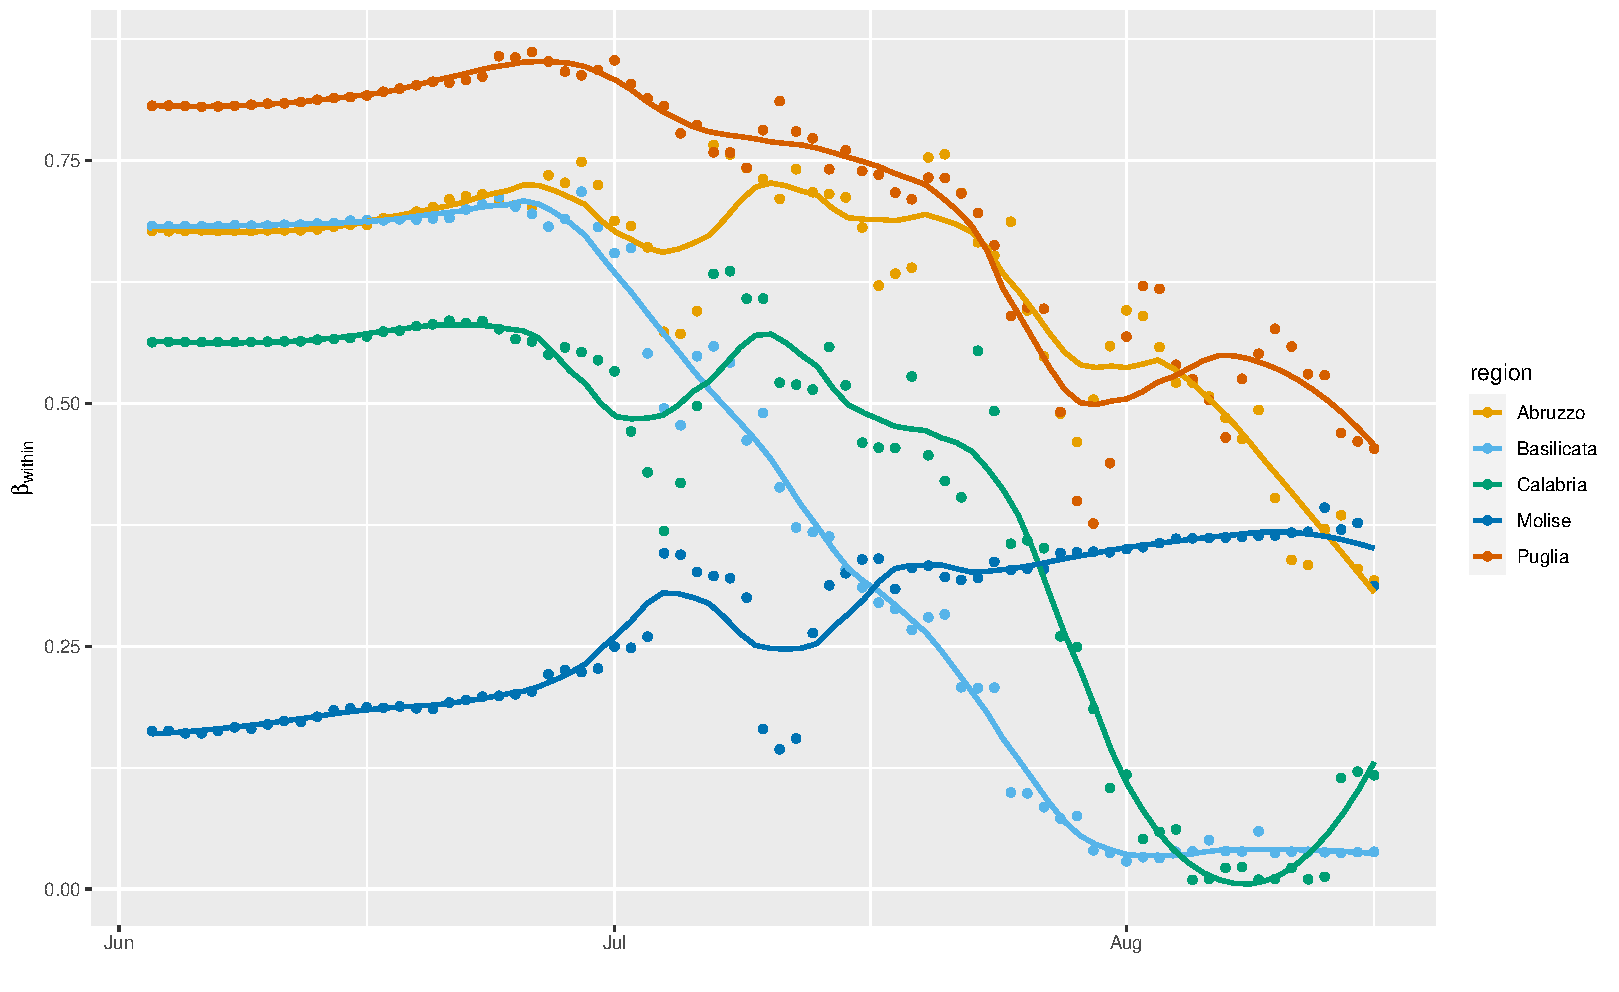
\includegraphics[width=0.95\linewidth]{output/model1_lag3_betawithin_Sud_aic_UndocQuadratic_rolling.pdf}
    	      \caption{With model selection by AIC; \\ including undocumented infectives}
    	      \label{fig:beta_within_over_time_sud_aic_undoc}
    	    \end{subfigure}
    	    \caption{Progression of $\beta_{within}$ over time for the \textit{Sud} (South) NUTS 1 region}
    	    \label{fig:beta_within_over_time_sud}
	    \end{figure}
		
		\begin{figure}[H]
    	    \centering
    	    \begin{subfigure}{\textwidth}
    	      \centering
    	      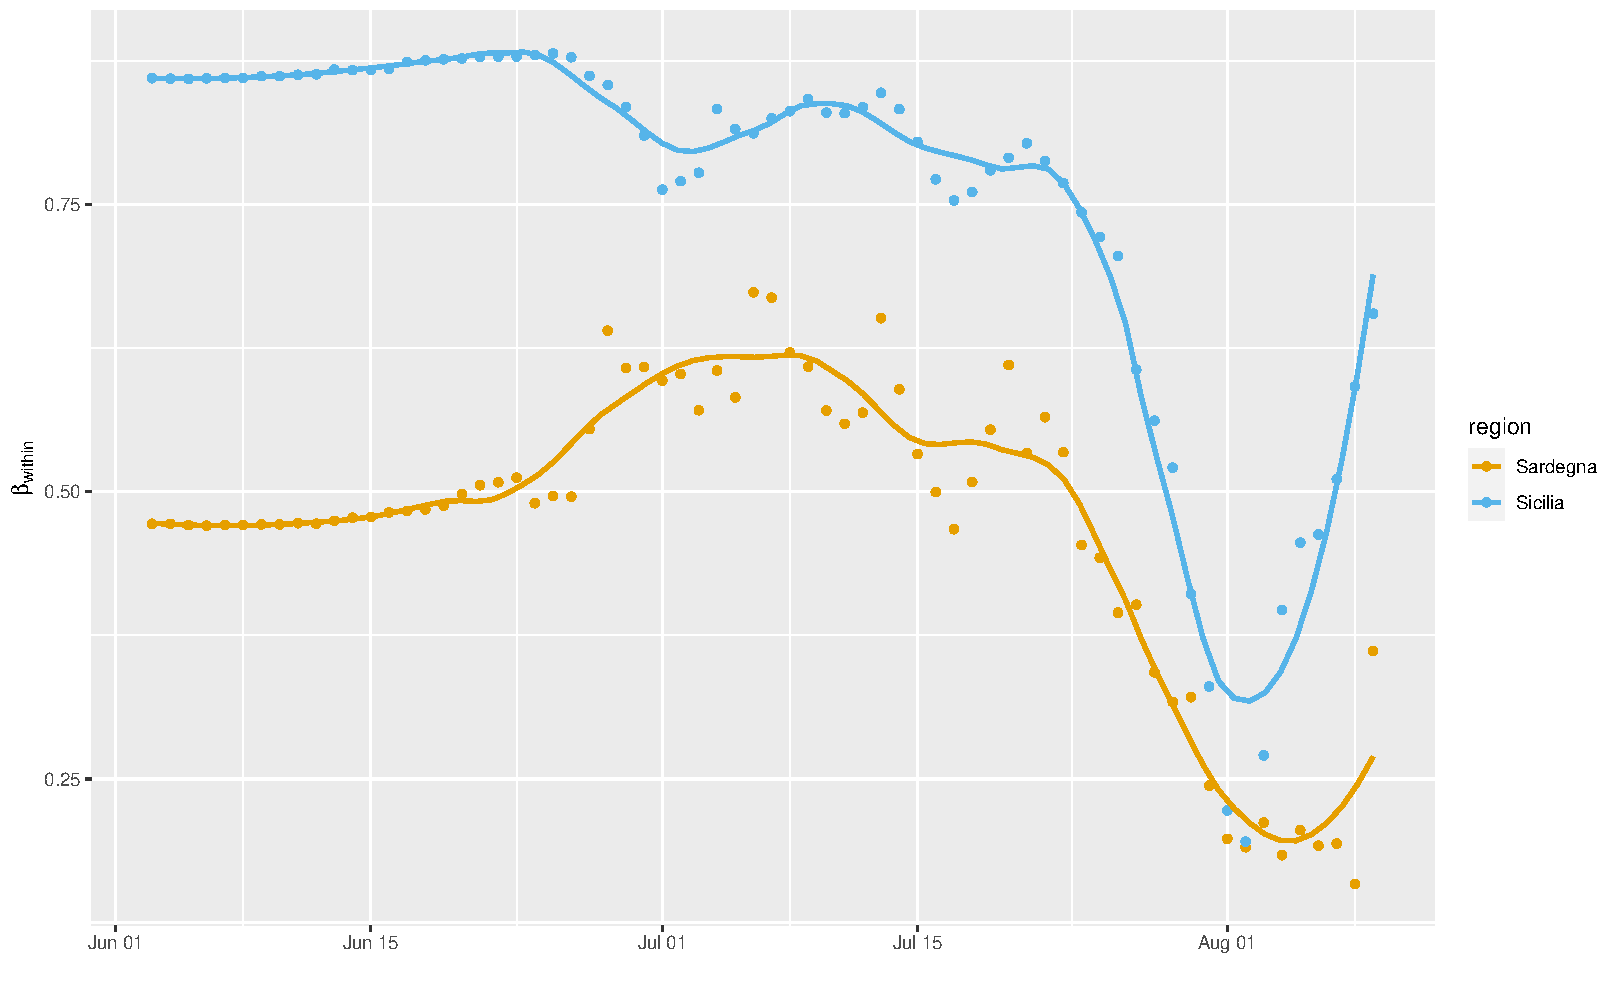
\includegraphics[width=0.95\linewidth]{output/model1_lag3_betawithin_Isole_rolling.pdf}
    	      \caption{Without model selection}
    	      \label{fig:beta_within_over_time_isole_regular}
    	    \end{subfigure}\newline
    	    \begin{subfigure}{\textwidth}
    	      \centering
    	      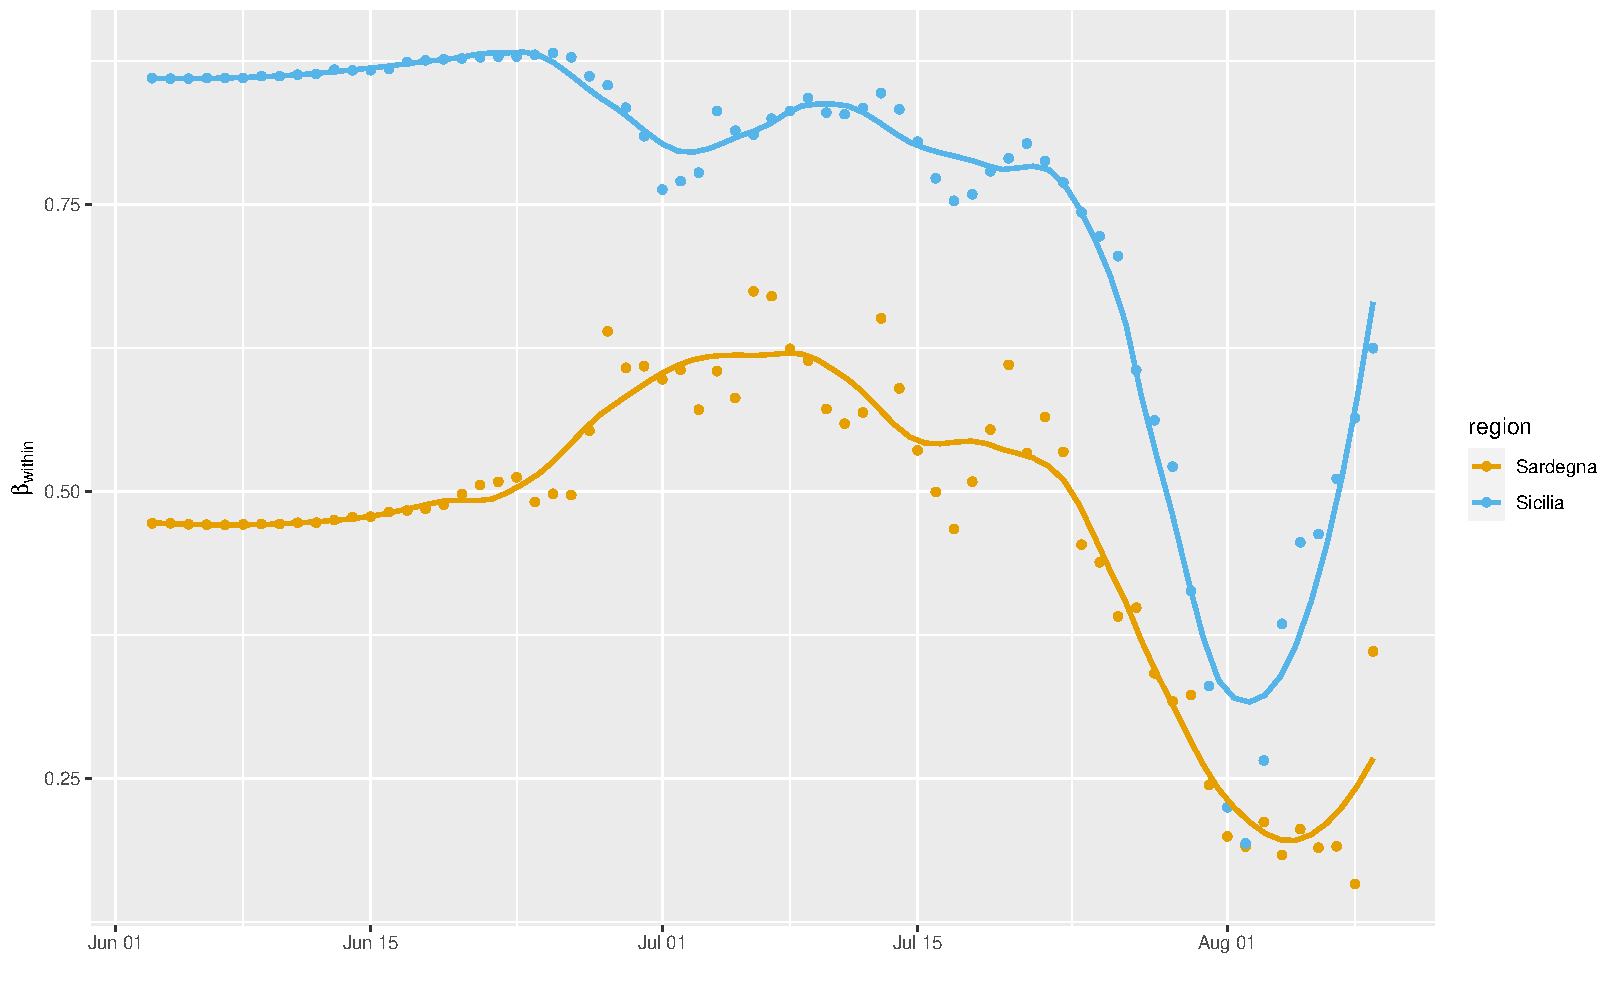
\includegraphics[width=0.95\linewidth]{output/model1_lag3_betawithin_Isole_aic_rolling.pdf}
    	      \caption{With model selection by AIC}
    	      \label{fig:beta_within_over_time_isole_aic}
    	    \end{subfigure}
    	\end{figure}
        \begin{figure}[H]\ContinuedFloat
    	    \begin{subfigure}{\textwidth}
    	      \centering
    	      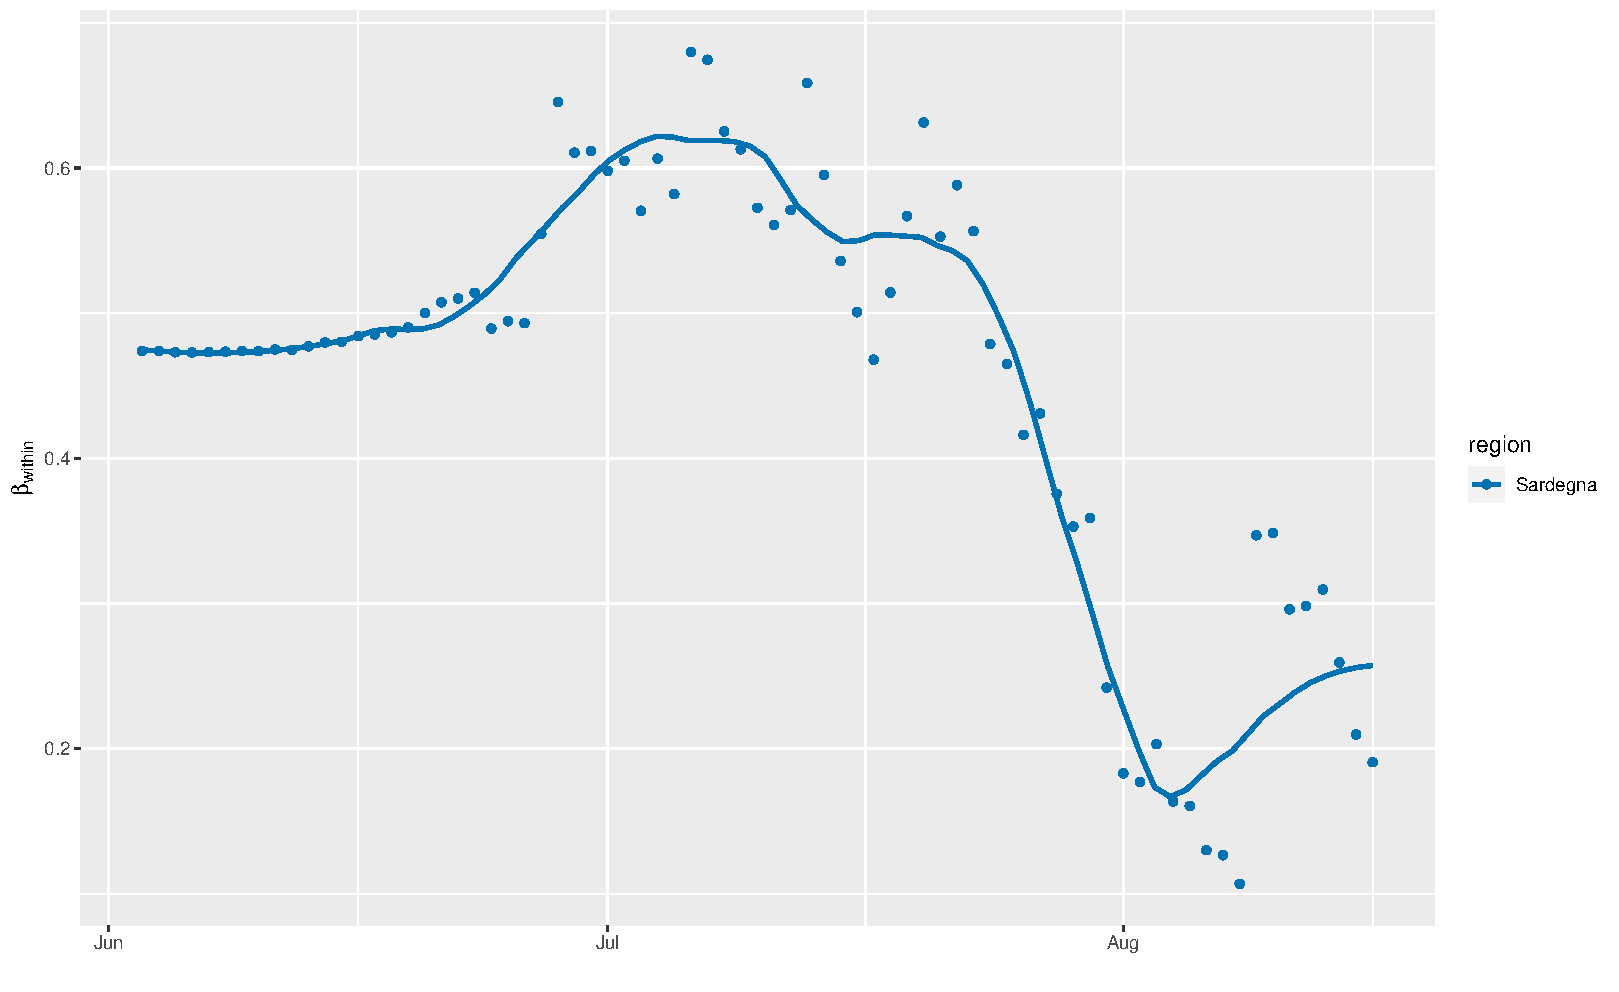
\includegraphics[width=0.95\linewidth]{output/model1_lag3_betawithin_Isole_UndocQuadratic_rolling.pdf}
    	      \caption{Without model selection; \\ including undocumented infectives}
    	      \label{fig:beta_within_over_time_isole_regular_undoc}
    	    \end{subfigure}\newline
    	    \begin{subfigure}{\textwidth}
    	      \centering
    	      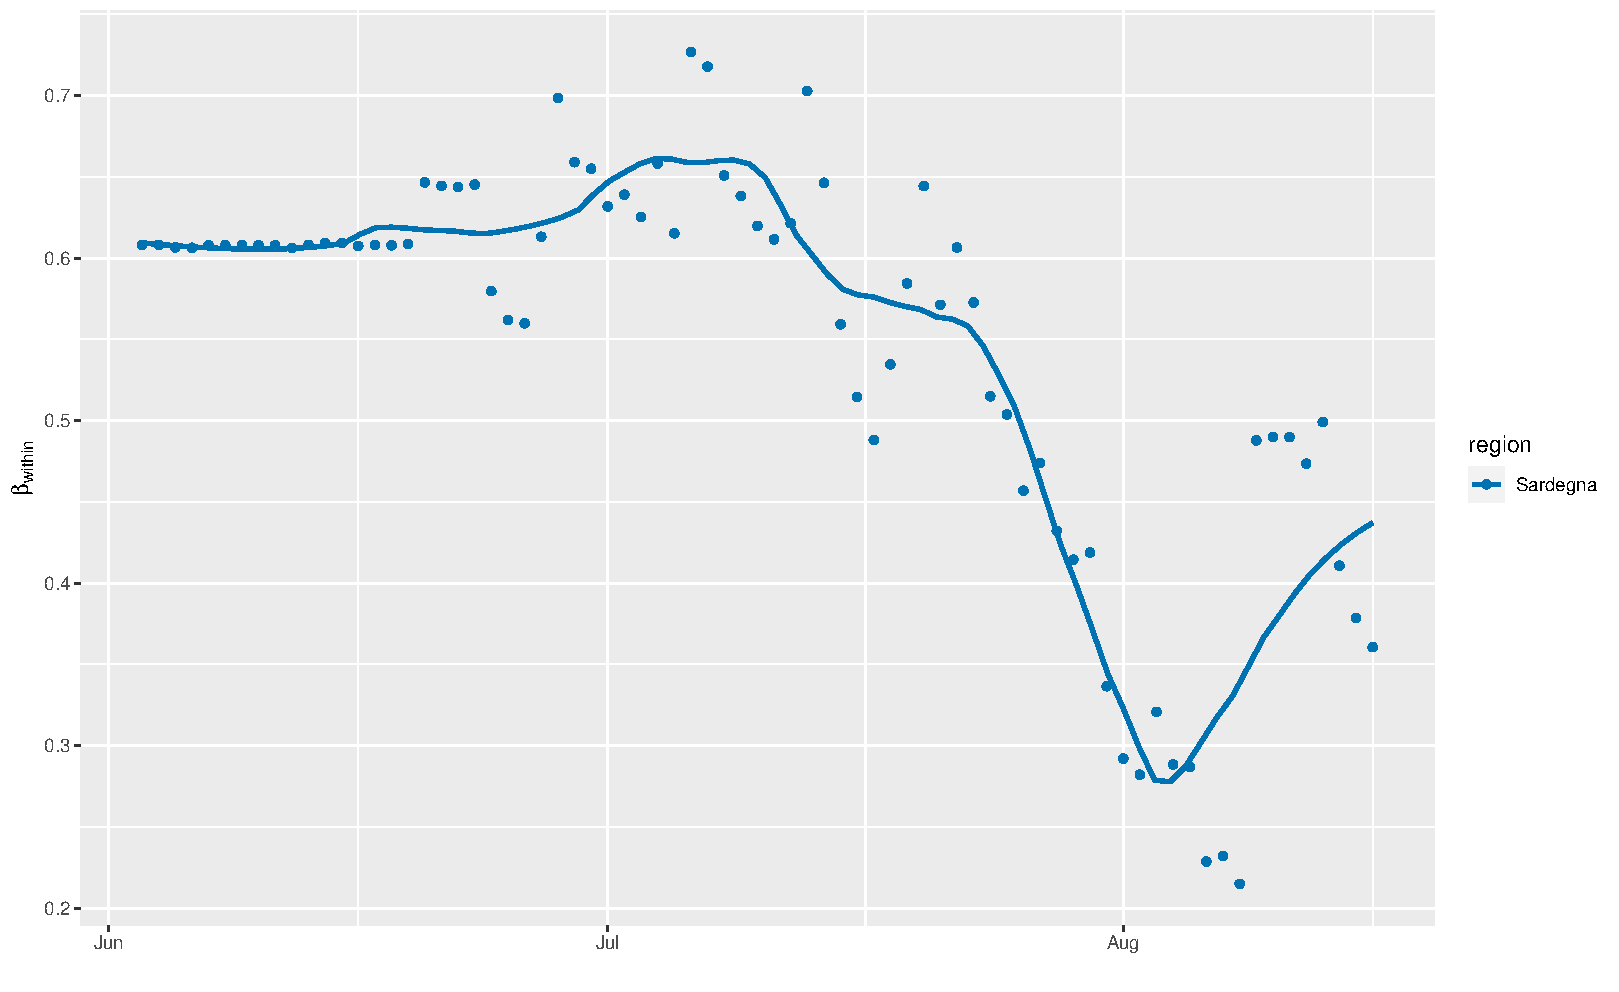
\includegraphics[width=0.95\linewidth]{output/model1_lag3_betawithin_Isole_aic_UndocQuadratic_rolling.pdf}
    	      \caption{With model selection by AIC; \\ including undocumented infectives}
    	      \label{fig:beta_within_over_time_isole_aic_undoc}
    	    \end{subfigure}
    	    \caption{Progression of $\beta_{within}$ over time for the \textit{Isole} (Islands) NUTS 1 region}
    	    \label{fig:beta_within_over_time_isole}
	    \end{figure}
		
		\subsection{Plots for Within and Between-Region Spread Model} \label{sapp:model3_plots}
		In Section \ref{subsec:results_within_between} we presented the plots of $\beta_{within}$ and $\beta_{between}$ over time for the \textit{Nord-Est} (North-East) NUTS 1 region for Within and Between-Region Spread Model. In this section, we present the plots for the other NUTS 1 regions. As is the case for Section \ref{subsec:results_within_between}, we use the last 100 observations.
		
		\begin{figure}[H]
    	    \centering
    	    \begin{subfigure}{\textwidth}
    	      \centering
    	      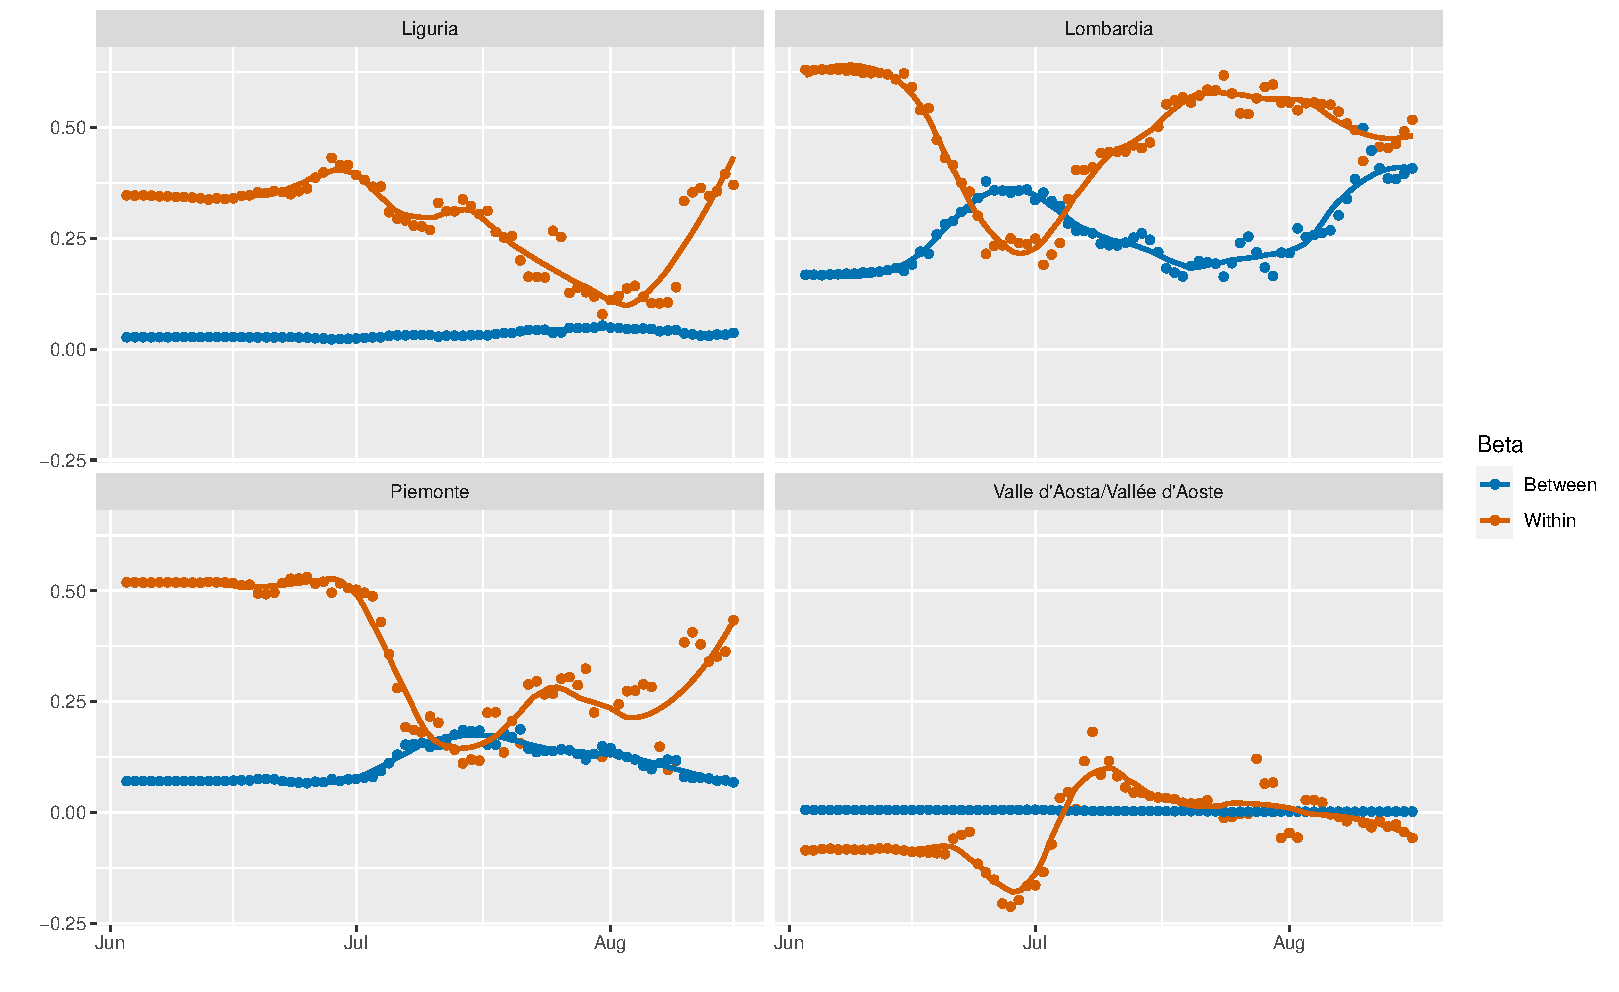
\includegraphics[width=0.95\linewidth]{output/model3_lag3_betas_Nord-Ovest_rolling.pdf}
    	      \caption{Without model selection}
    	      \label{fig:beta_within_between_over_time_nordovest_regular}
    	    \end{subfigure}\newline
    	    \begin{subfigure}{\textwidth}
    	      \centering
    	      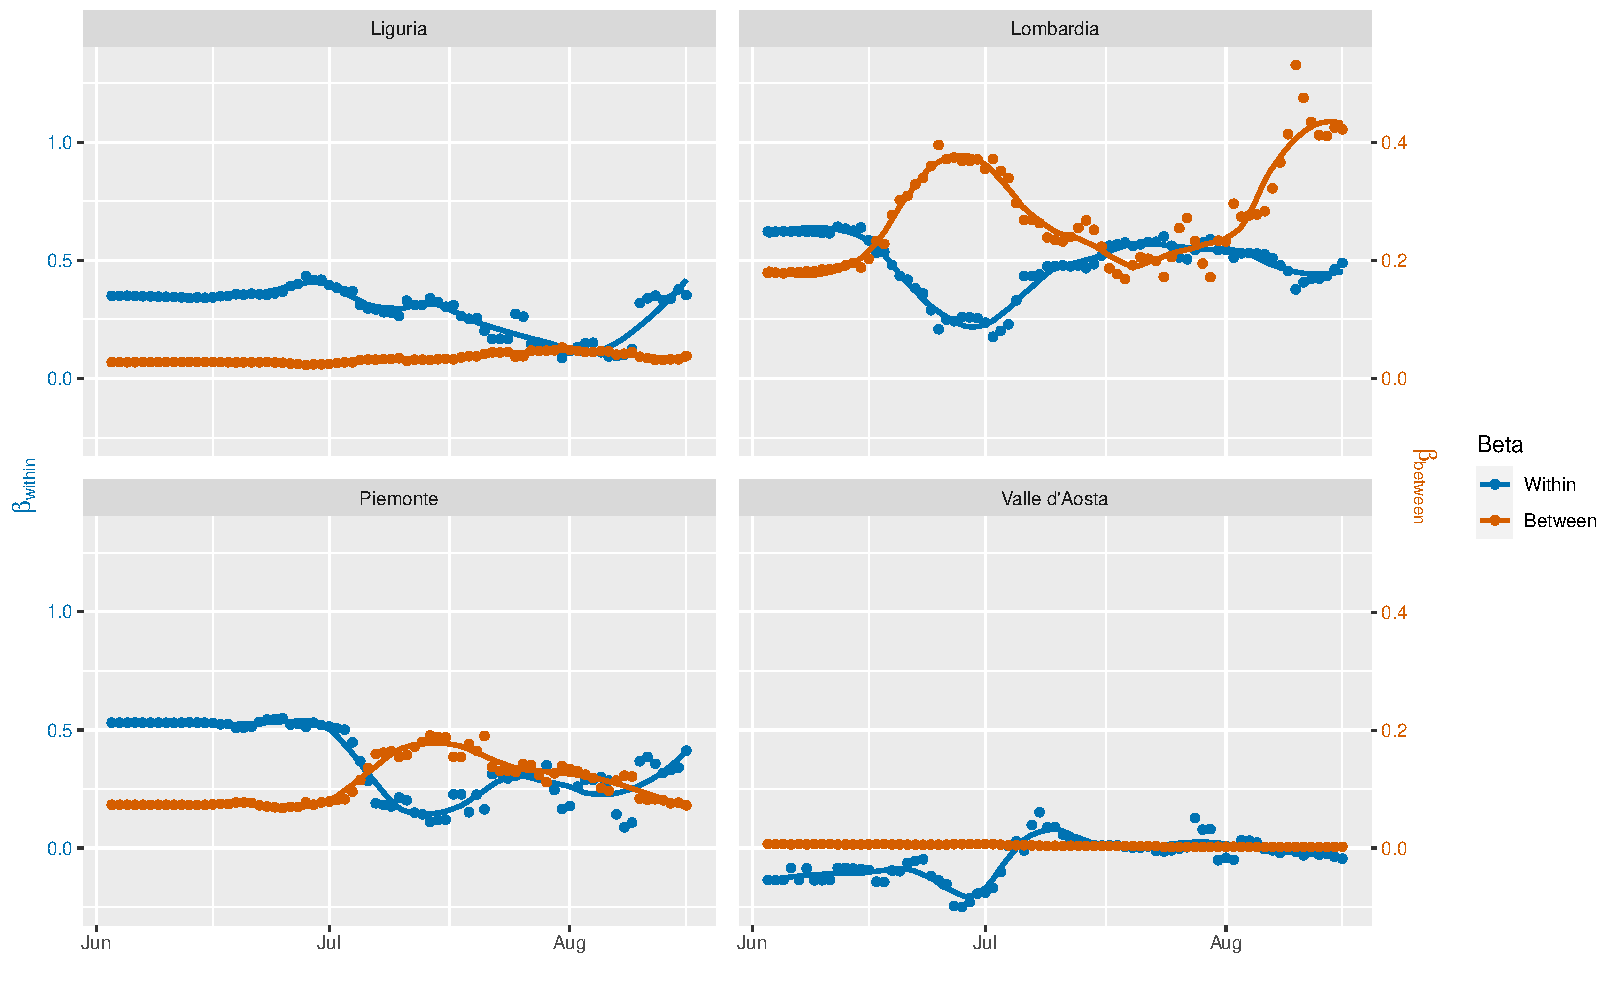
\includegraphics[width=0.95\linewidth]{output/model3_lag3_betas_Nord-Ovest_aic_rolling.pdf}
    	      \caption{With model selection by AIC}
    	      \label{fig:beta_within_between_over_time_nordovest_aic}
    	    \end{subfigure}
    	\end{figure}
        \begin{figure}[H]\ContinuedFloat
    	    \begin{subfigure}{\textwidth}
    	      \centering
    	      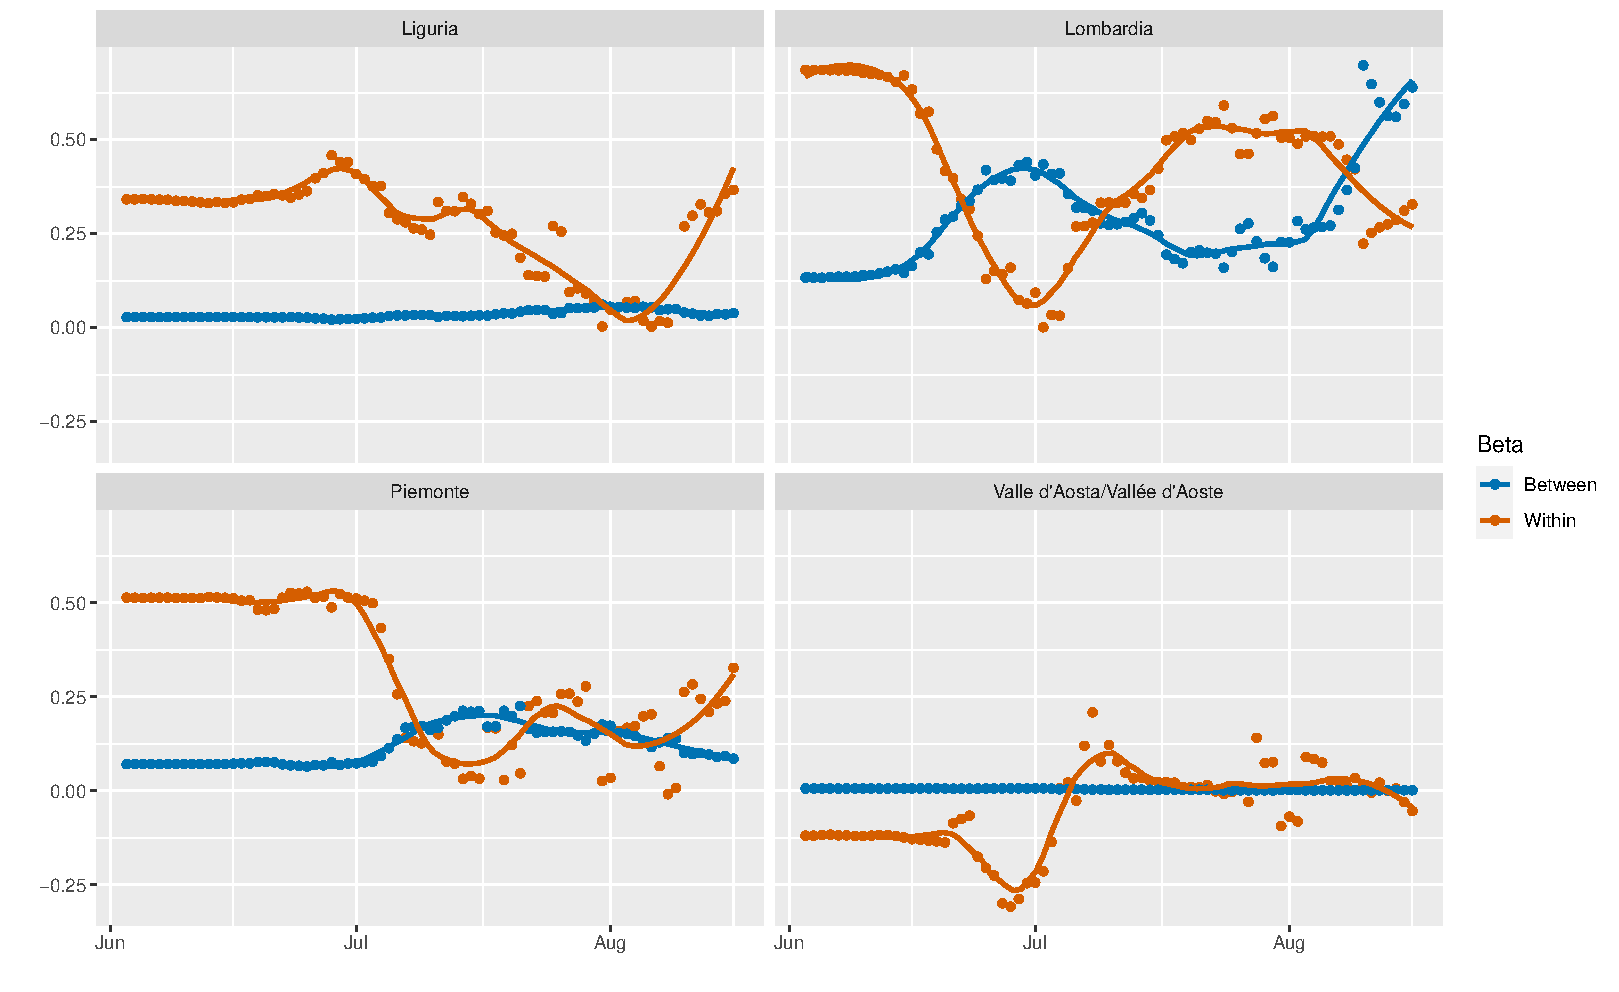
\includegraphics[width=0.95\linewidth]{output/model3_lag3_betas_Nord-Ovest_UndocQuadratic_rolling.pdf}
    	      \caption{Without model selection; \\ including undocumented infectives}
    	      \label{fig:beta_within_between_over_time_nordovest_regular_undoc}
    	    \end{subfigure}\newline
    	    \begin{subfigure}{\textwidth}
    	      \centering
    	      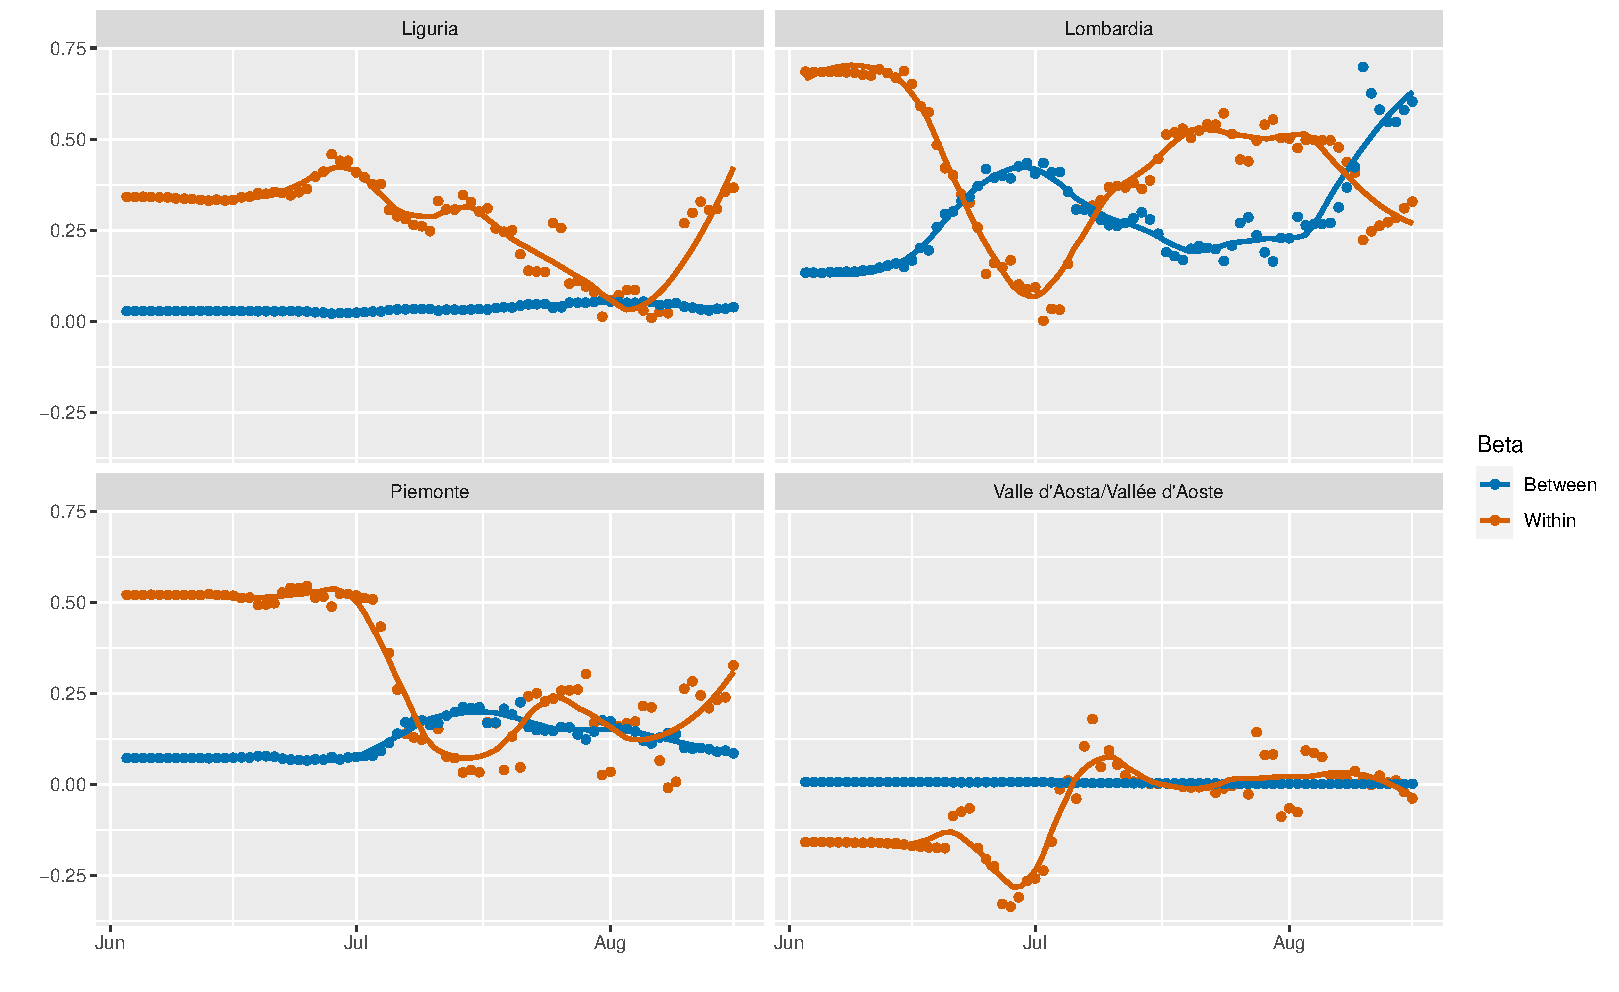
\includegraphics[width=0.95\linewidth]{output/model3_lag3_betas_Nord-Ovest_aic_UndocQuadratic_rolling.pdf}
    	      \caption{With model selection by AIC; \\ including undocumented infectives}
    	      \label{fig:beta_within_between_over_time_nordovest_aic_undoc}
    	    \end{subfigure}
    	    \caption{Progression of $\beta_{within}$ and $\beta_{between}$ over time for the \textit{Nord-Ovest} (North-West) NUTS 1 region}
    	    \label{fig:beta_within_between_over_time_nordovest}
        \end{figure}
		
		\begin{figure}[H]
    	    \centering
    	    \begin{subfigure}{\textwidth}
    	      \centering
    	      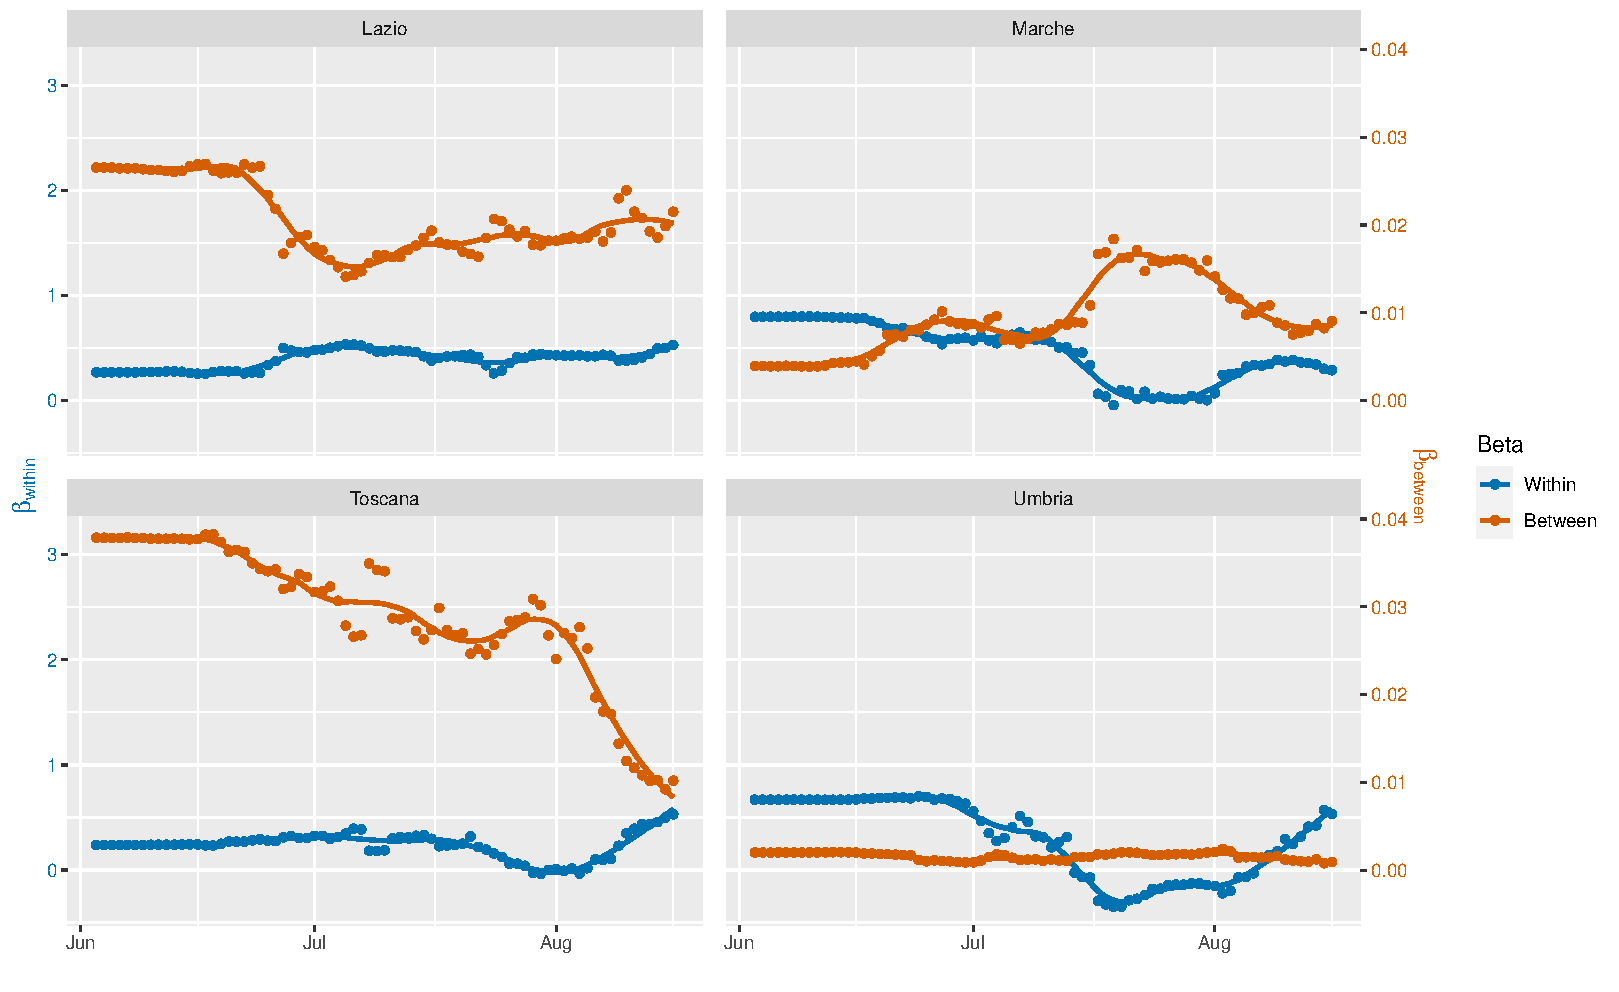
\includegraphics[width=0.95\linewidth]{output/model3_lag3_betas_Centro (IT)_rolling.pdf}
    	      \caption{Without model selection}
    	      \label{fig:beta_within_between_over_time_centro_regular}
    	    \end{subfigure}\newline
    	    \begin{subfigure}{\textwidth}
    	      \centering
    	      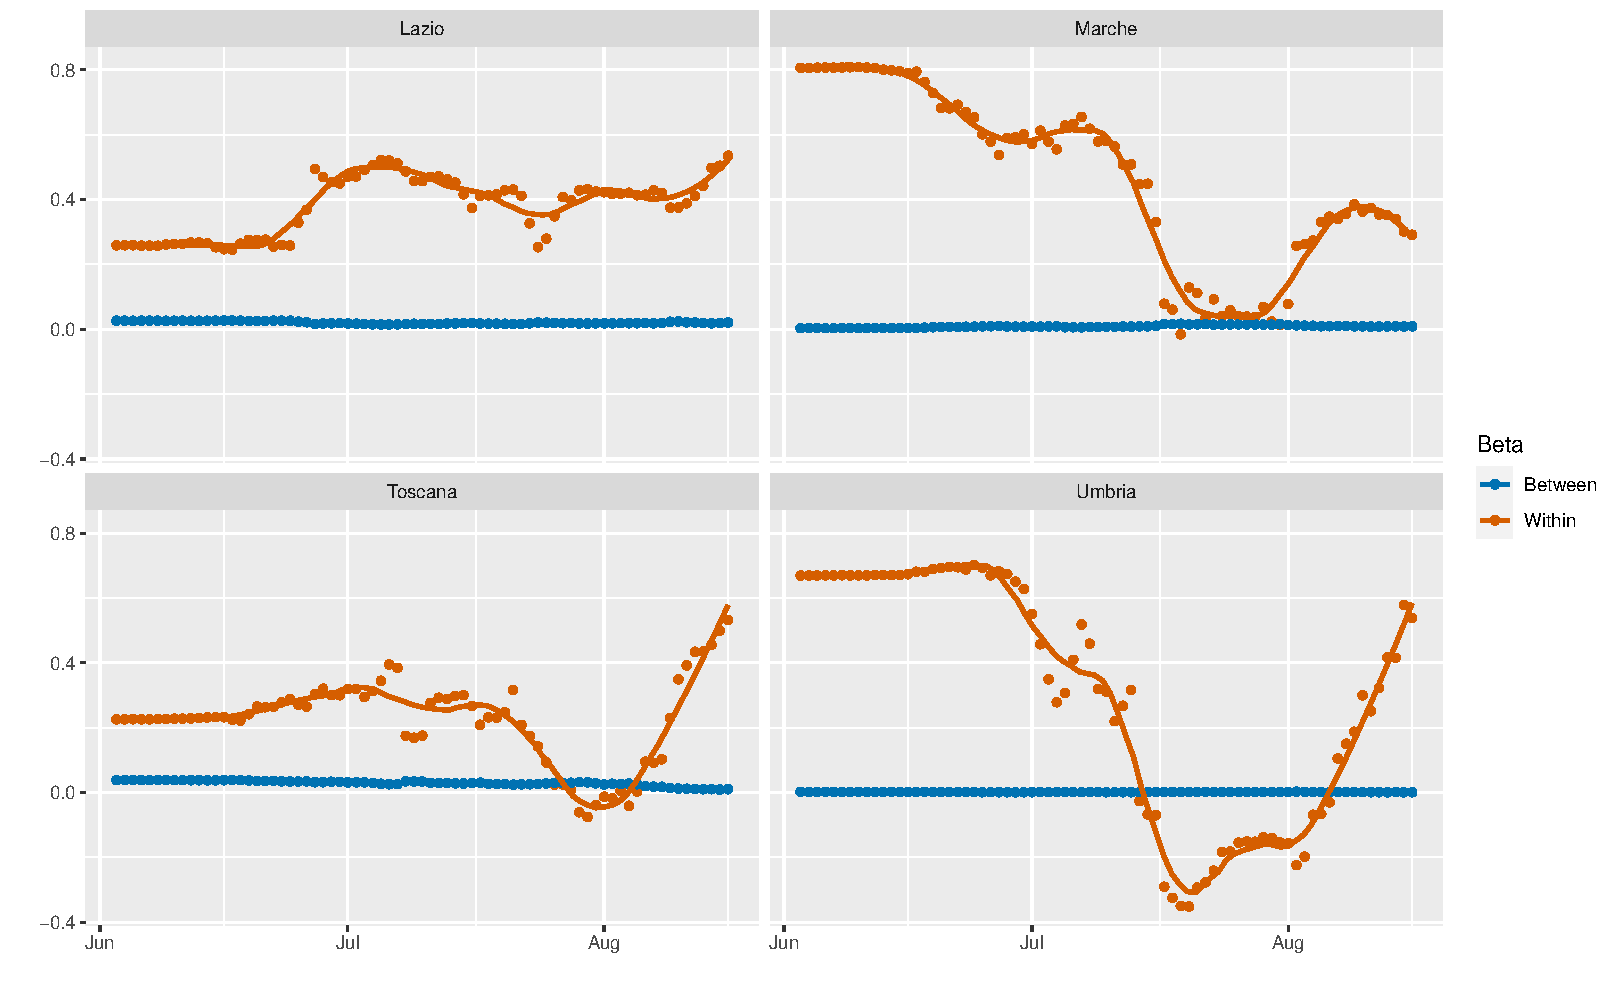
\includegraphics[width=0.95\linewidth]{output/model3_lag3_betas_Centro (IT)_aic_rolling.pdf}
    	      \caption{With model selection by AIC}
    	      \label{fig:beta_within_between_over_time_centro_aic}
    	    \end{subfigure}
    	\end{figure}
        \begin{figure}[H]\ContinuedFloat
    	    \begin{subfigure}{\textwidth}
    	      \centering
    	      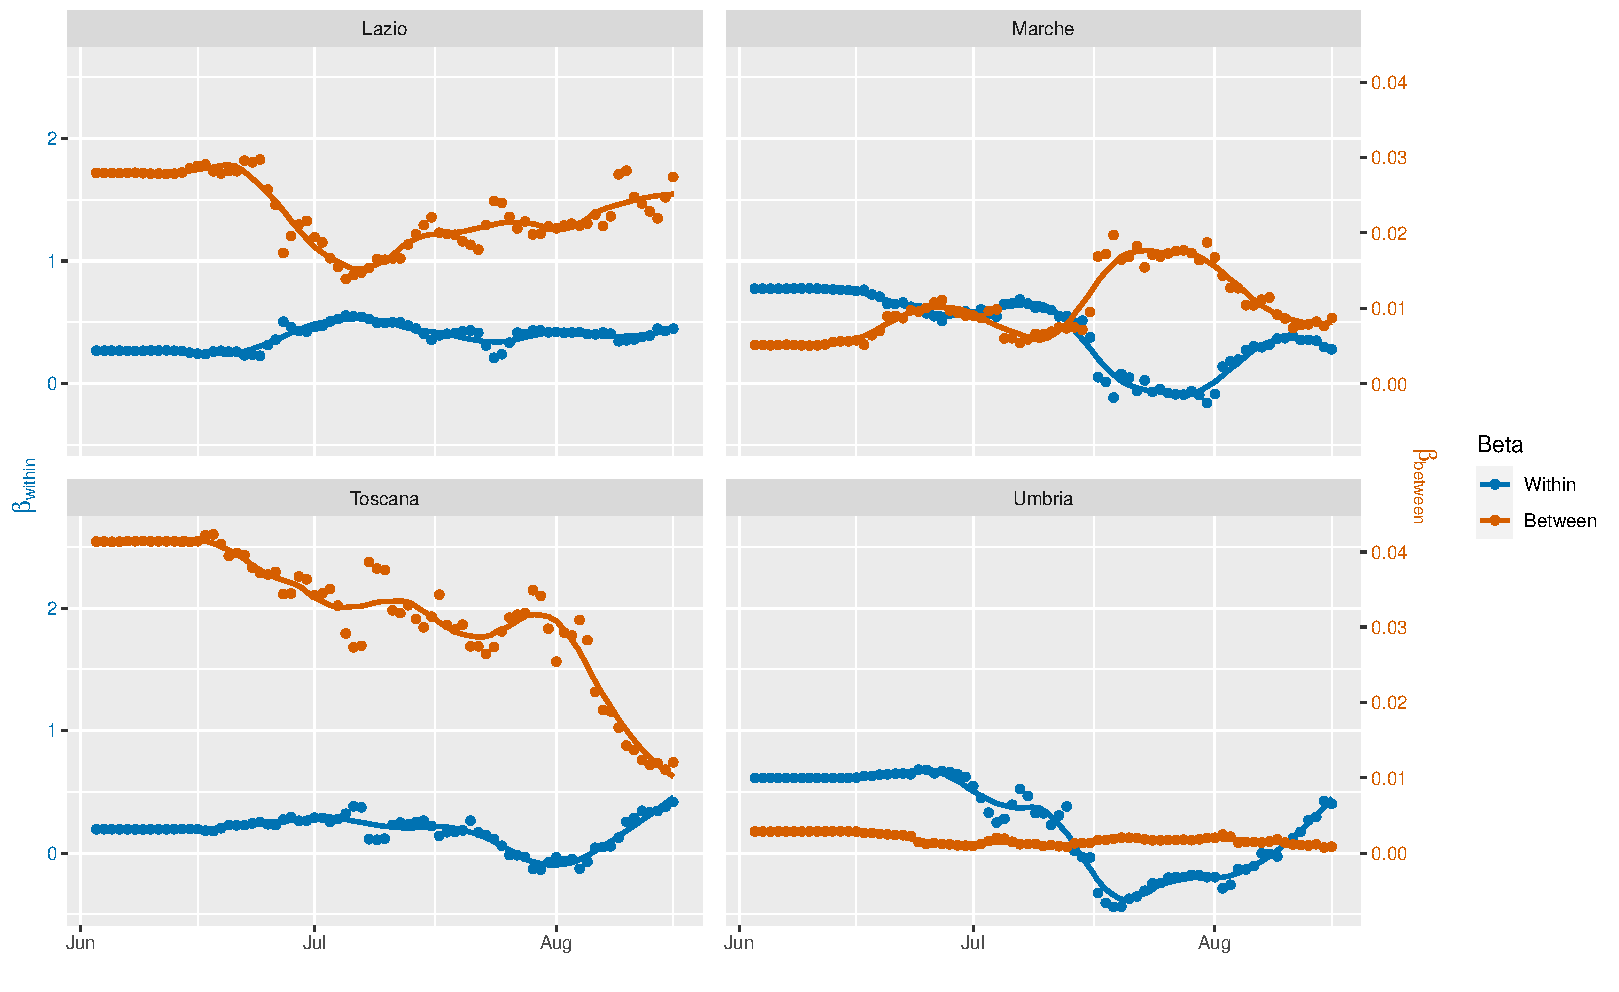
\includegraphics[width=0.95\linewidth]{output/model3_lag3_betas_Centro (IT)_UndocQuadratic_rolling.pdf}
    	      \caption{Without model selection; \\ including undocumented infectives}
    	      \label{fig:beta_within_between_over_time_centro_regular_undoc}
    	    \end{subfigure}\newline
    	    \begin{subfigure}{\textwidth}
    	      \centering
    	      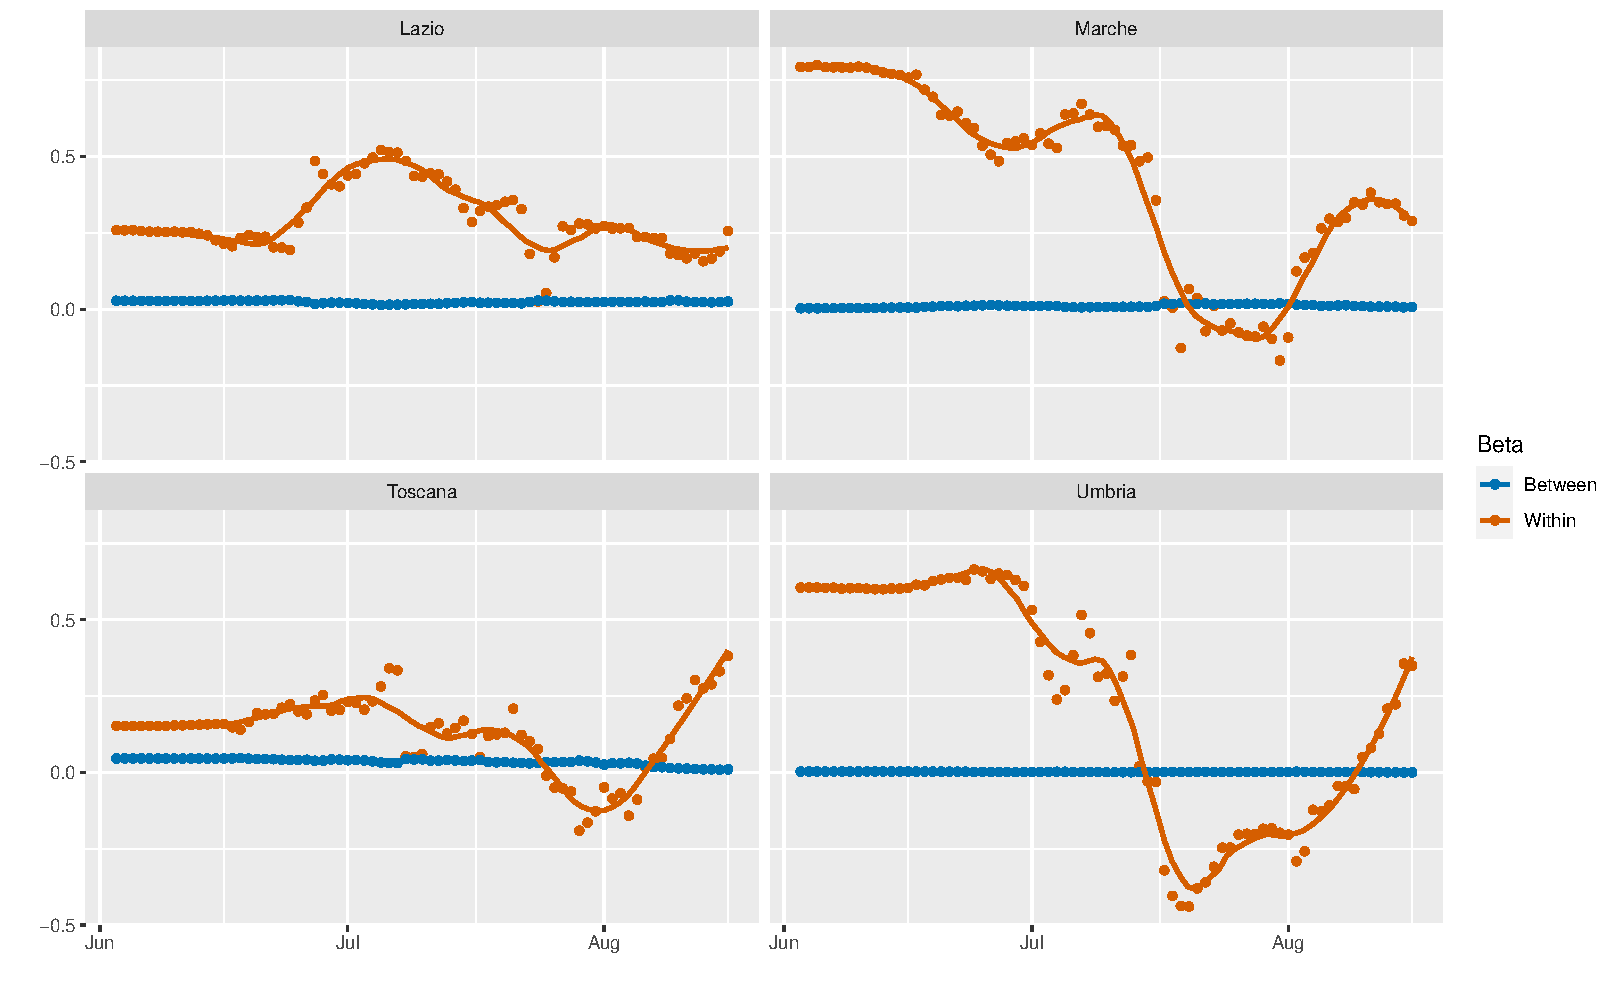
\includegraphics[width=0.95\linewidth]{output/model3_lag3_betas_Centro (IT)_aic_UndocQuadratic_rolling.pdf}
    	      \caption{With model selection by AIC; \\ including undocumented infectives}
    	      \label{fig:beta_within_between_over_time_centro_aic_undoc}
    	    \end{subfigure}
    	    \caption{Progression of $\beta_{within}$ and $\beta_{between}$ over time for the \textit{Centro (IT)} (Centre) NUTS 1 region}
    	    \label{fig:beta_within_between_over_time_centro}
        \end{figure}
		
		\begin{figure}[H]
    	    \centering
    	    \begin{subfigure}{\textwidth}
    	      \centering
    	      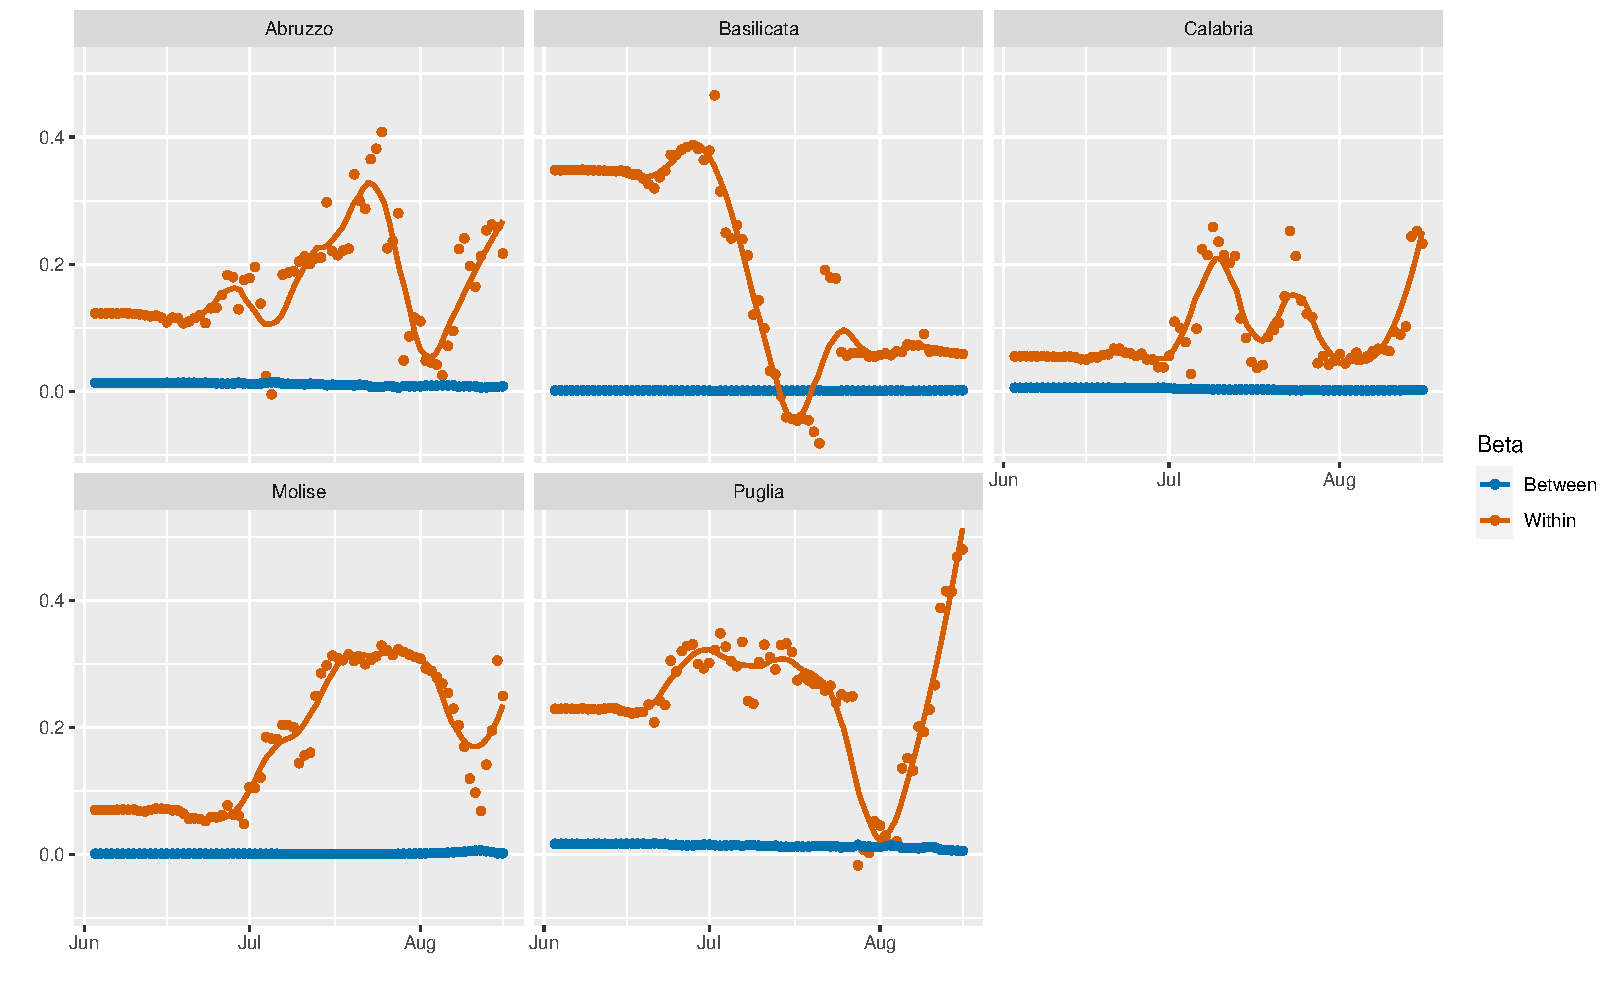
\includegraphics[width=0.95\linewidth]{output/model3_lag3_betas_Sud_rolling.pdf}
    	      \caption{Without model selection}
    	      \label{fig:beta_within_between_over_time_sud_regular}
    	    \end{subfigure}\newline
    	    \begin{subfigure}{\textwidth}
    	      \centering
    	      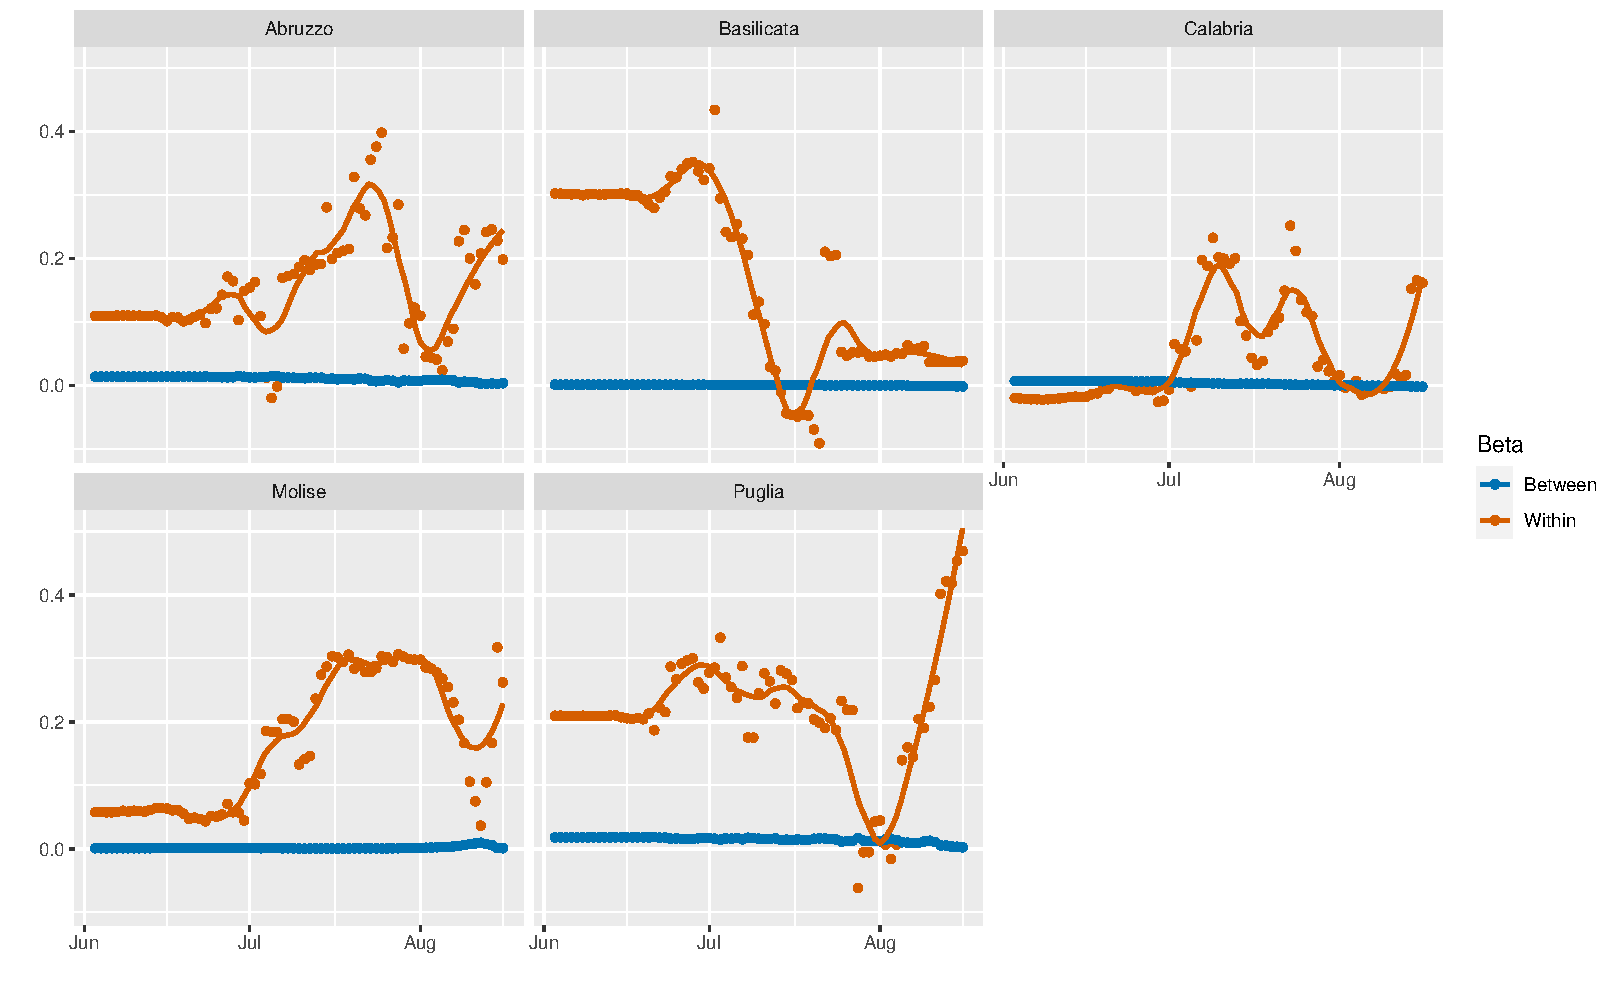
\includegraphics[width=0.95\linewidth]{output/model3_lag3_betas_Sud_aic_rolling.pdf}
    	      \caption{With model selection by AIC}
    	      \label{fig:beta_within_between_over_time_sud_aic}
    	    \end{subfigure}
    	\end{figure}
        \begin{figure}[H]\ContinuedFloat
    	    \begin{subfigure}{\textwidth}
    	      \centering
    	      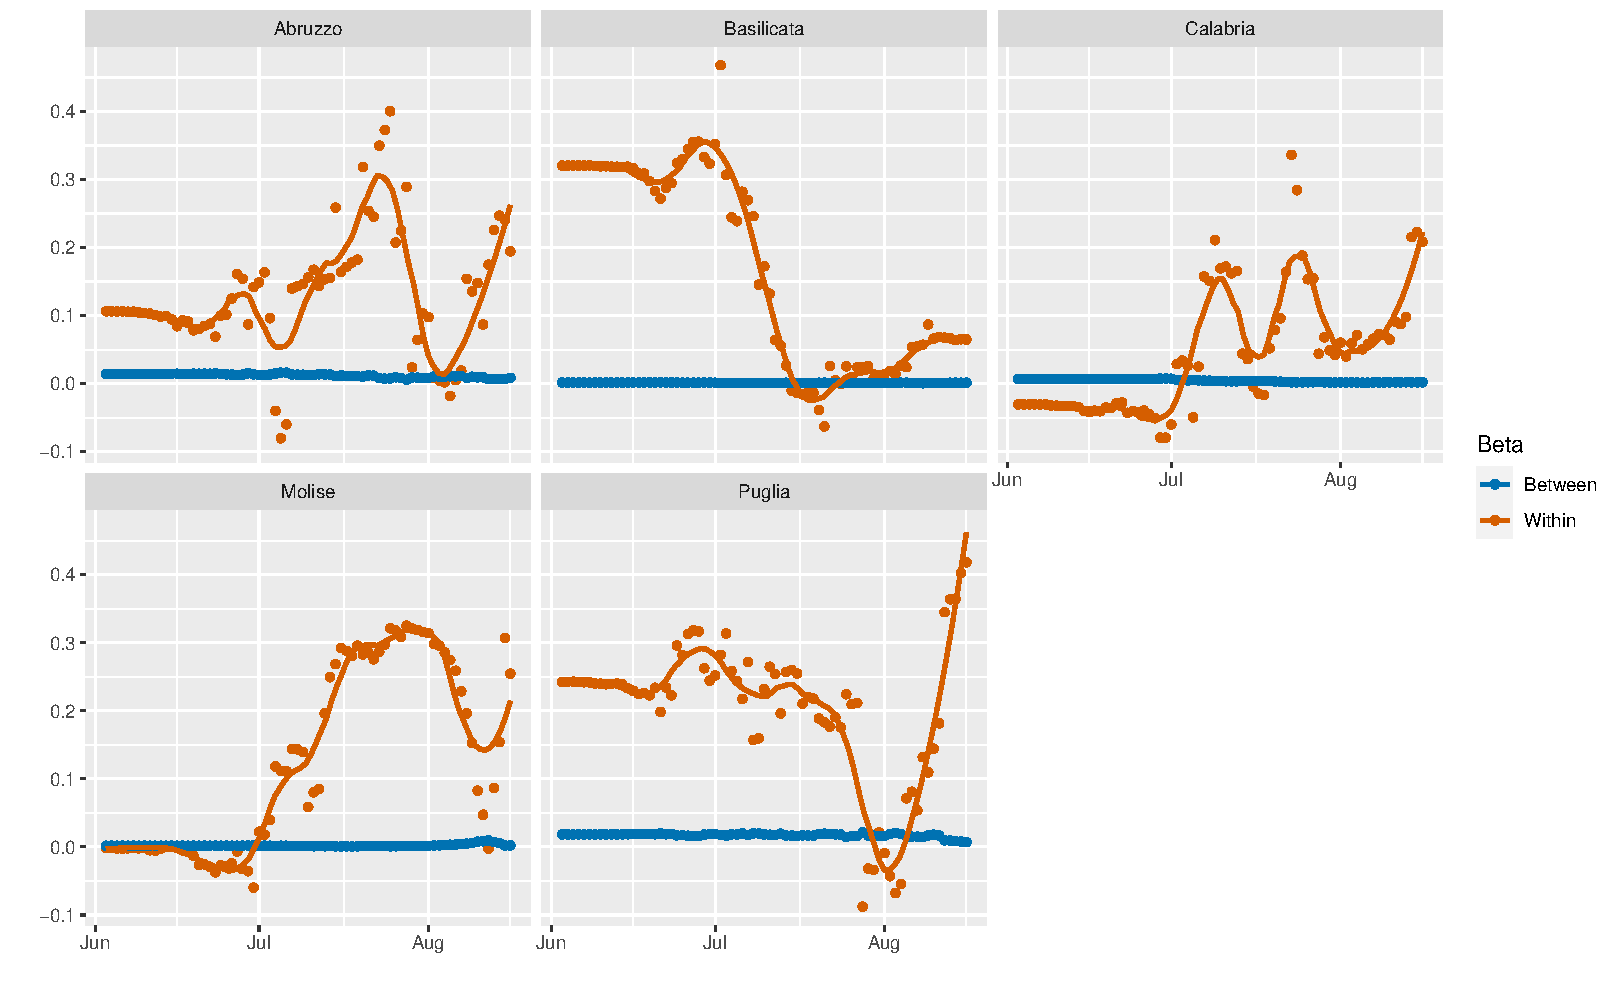
\includegraphics[width=0.95\linewidth]{output/model3_lag3_betas_Sud_UndocQuadratic_rolling.pdf}
    	      \caption{Without model selection; \\ including undocumented infectives}
    	      \label{fig:beta_within_between_over_time_sud_regular_undoc}
    	    \end{subfigure}\newline
    	    \begin{subfigure}{\textwidth}
    	      \centering
    	      \includegraphics[width=0.95\linewidth]{output/model3_lag3_betas_Sud_aic_UndocQuadratic_rolling.pdf}
    	      \caption{With model selection by AIC; \\ including undocumented infectives}
    	      \label{fig:beta_within_between_over_time_sud_aic_undoc}
    	    \end{subfigure}
    	    \caption{Progression of $\beta_{within}$ and $\beta_{between}$ over time for the \textit{Centro (IT)} (Centre) NUTS 1 region}
    	    \label{fig:beta_within_between_over_time_sud}
        \end{figure}
		
		\newpage
		\section{Derivations} \label{app:derivations}
		
		\subsection{Calculation of population variables}\label{sapp:derivation_population_variables}
		In this appendix, we will explain how the susceptible population and total population are calculated. Unfortunately, we do not have data on the total population per day. For this reason, we retrieve the latest population numbers per region from \textcite{eurostatDatabase}, which are from January 1, 2019, and the yearly population growth rates for 2019 and 2020 from \textcite{worldometer2020italypopulation}. For 2019, growth rate was equal to -0.13\% and for 2020, excluding the deaths due to the pandemic, it was estimated to be equal to -0.15\%. We only have the population growth rates available for the whole of Italy, not per region, unfortunately. As such, we assume that the growth rates are uniformly applicable to all regions. Of course, this is likely to introduce a small error since these growth rates differ over the regions. We assume that this error is negligible. \\
		
		We denote the population of region $r$ at time $t$ by $N_{r,t}$. We denote the yearly population growth rates for 2019 and 2020 by $g_{2019}$ and $g_{2020}$, respectively. Lastly, recall that the data for the pandemic starts at February 25, 2020. This is the 54\textsuperscript{th} day of 2020, a leap year. As such, the population of region $r$ on February 25, 2020 is calculated as:
		\begin{equation}\label{eq:calc_total_population}
		    N_{r, 2020\shortminus02\shortminus25} = (1+g_{2019})(1+g_{2020})^{\frac{54}{366}}N_{r, 2019\shortminus01\shortminus01} - D_{r, 2020\shortminus02\shortminus25}
		\end{equation}
		where $D_{r,t}$ denotes the number of deaths in region $r$ at time $t$. \\
		
		Recall that the data reported at time $t$ is reported with respect to the last 24 hours. As such, the susceptible population at time $t$ can be calculated with the data at that same time. The susceptible population of region $r$ at time $t$, denoted by $X_{r,t}$, is therefore calculated as follows:
		\begin{equation}\label{eq:calc_susceptible_population}
		    X_{r,t} = N_{r,t} - Y_{r,t} - Z_{r,t}
		\end{equation}
		where $Y_{r,t}$ denotes the number of infectives and $Z_{r,t}$ denotes the number of removed individuals. Recall that $r$ is made up by adding the recovered individuals and the deceased individuals. Because we use the calculation of $N_{r,t}$ as in the previous paragraph, the error discussed propagates into the calculation of $X_{r,t}$. However, as before, we assume that this error is negligible.
		
		\subsection{Functional forms for modelling undocumented infectives}\label{sapp:derivation_undocumented_infectives}
		In this appendix, we give the derivations for the functional forms for modelling undocumented infectives as discussed in Section \ref{sec:undocumented_modelling}.
		
		\subsubsection{Linear function} \label{ssapp:linear_derivation}
		For modelling the undocumented infectives, we want to construct a formula for a linear function that obeys the following assumptions:
		\begin{enumerate}[label=(\Roman*)]
		    \item\label{ass:linear_formula} $f(TC_t) = aTC_t + b$  for some $a, b \in \R$,
		    \item\label{ass:linear_0} $f(0) = f^{min}$ for some $f^{min} \in [0,1]$,
		    \item\label{ass:linear_N} $f(N_t) = 1$
		\end{enumerate}
		
		From assumption \ref{ass:linear_0}, we obtain that $b = f^{min}$. From assumption \ref{ass:linear_N}, we can then derive the value of $a$. The equation that we need to solve is:
		    \[aN_t + f^{min} = 1.\]
		    
		This is readily solved as $a = \frac{1-f^{min}}{N_t}$. As such, we have derived that
		    \[f(TC_t) = \frac{1-f^{min}}{N_t}TC_t + f^{min}.\]
		
		\subsubsection{General quadratic function} \label{ssapp:quadratic_derivation}
		For modelling the undocumented infectives, we want to construct a general formula for a quadratic function that obeys the following assumptions:
		\begin{enumerate}[label=(\Roman*)]
		    \item\label{ass:parabola_formula} $f(TC_t) = aTC_t^2 + bTC_t + c$ for some $a, b, c \in \R$,
		    \item\label{ass:parabola_0} $f(0) = f^{min}$ for some $f^{min} \in [0,1]$,
		    \item\label{ass:parabola_N} $f(N_t) = 1$,
		    \item\label{ass:parabola_betaN} $f(\beta N_t) = \gamma$ for some $\beta, \gamma \in (0,1)$,
		    \item\label{ass:parabola_vertex} The vertex of the parabola should be to the right of $N_t$ in the case of a downwards opening parabola and to the left of the origin in the case of an upwards opening parabola.
		\end{enumerate}
		
		From assumption \ref{ass:parabola_0}, we obtain that $c = f^{min}$. From assumptions \ref{ass:parabola_N} and \ref{ass:parabola_betaN}, we can then derive the values of $a$ and $b$ in terms of $\beta$, $\gamma$ and $N_t$. The set of equations that we need to solve are:
		
		\begin{equation} \label{eq:set_parabola}
		    \begin{cases}
		        aN_t^2 + bN_t + f^{min} &= 1 \text{ (from assumption \ref{ass:parabola_N})}\\
		        a\beta^2 N_t^2 + b\beta N_t + f^{min} &= \gamma \text{ (from assumption \ref{ass:parabola_betaN})}
		    \end{cases}
		\end{equation}
		
		To solve \eqref{eq:set_parabola}, we can apply row reduction as follows:
		
		\begin{alignat*}{2}
            \begin{sysmatrix}{cc|c}
            N_t^2 & N_t & 1 - f^{min} \\
            \beta^2 N_t^2 & \beta N_t & \gamma - f^{min} \\
            \end{sysmatrix}
            &\!\begin{aligned}
            &\ro{r_2 - \beta^2 r_1}
            \end{aligned}
            \begin{sysmatrix}{cc|c}
            N_t^2 & N_t & 1 - f^{min} \\
            0 & \beta(1-\beta) N_t & \gamma - f^{min} - \beta^2 + \beta^2 f^{min} \\
            \end{sysmatrix}
            \\
            &\!\begin{aligned}
            &\ro{r_2 \div \beta(1-\beta)}
            \end{aligned}
            \begin{sysmatrix}{cc|c}
            N_t^2 & N_t & 1 - f^{min} \\
            0 & N_t & \frac{\gamma - f^{min} - \beta^2 + \beta^2 f^{min}}{\beta(1-\beta)} \\
            \end{sysmatrix}
            \\
            &\!\begin{aligned}
            &\ro{r_1 - r_2}
            \end{aligned}
            \begin{sysmatrix}{cc|c}
            N_t^2 & 0 & \frac{\beta - \gamma + (1-\beta)f^{min}}{\beta(1-\beta)} \\
            0 & N_t & \frac{\gamma - f^{min} - \beta^2 + \beta^2 f^{min}}{\beta(1-\beta)} \\
            \end{sysmatrix}
            \\
            &\!\begin{aligned}
            &\ro{r_1 \div N_t^2}\\
            &\ro{r_2 \div N_t}
            \end{aligned}
            \begin{sysmatrix}{cc|c}
            1 & 0 & \frac{\beta - \gamma + (1-\beta)f^{min}}{\beta(1-\beta)N_t^2} \\
            0 & 1 & \frac{\gamma - f^{min} - \beta^2 + \beta^2 f^{min}}{\beta(1-\beta)N_t} \\
            \end{sysmatrix}
        \end{alignat*}
        
        As such, we have derived that
        \begin{equation} \label{eq:parabola_a_b}
		    \begin{cases}
		        a &= \frac{\beta - \gamma + (1-\beta)f^{min}}{\beta(1-\beta)N_t^2} \\
		        b &= \frac{\gamma - f^{min} - \beta^2 + \beta^2 f^{min}}{\beta(1-\beta)N_t} \\
		        c &= f^{min}.
		    \end{cases}
		\end{equation}
        
        Firstly, note that this function is an upwards opening parabola if $a>0$ and a downwards opening parabola if $a<0$. For instance, we have that:
        \begin{align*}
            & a > 0 \\
            \iff & \frac{\beta - \gamma + (1-\beta)f^{min}}{\beta(1-\beta)N_t^2} > 0 \\
            \iff & \beta - \gamma + (1-\beta)f^{min} > 0 \\
            \iff & \gamma < \beta + (1-\beta)f^{min}
        \end{align*}
        where we use that $\beta(1-\beta)N_t^2 > 0$. Similarly, we have that $a < 0$ if $\gamma > \beta + (1-\beta)f^{min}$. \\
        
        Now note that our function is continuous. As such, we assume without loss of generality that $\beta = \frac{1}{2}$ and do the following derivations to deduce the values of $\gamma$ for which assumption \ref{ass:parabola_vertex} holds. That is, we want to find the values of $\gamma$ for which
        \begin{equation*}
            f'(TC_t) = 0 \iff 
		    \begin{cases}
		        TC_t &\geq N_t \text{ for } \gamma > \frac{1}{2} + \frac{1}{2}f^{min} \\
		        TC_t &\leq 0 \text{ for } \gamma < \frac{1}{2} + \frac{1}{2}f^{min}.
		    \end{cases}
		\end{equation*}
		
		Firstly, assuming $\beta = \frac{1}{2}$, the expressions for $a$ and $b$ as in \eqref{eq:parabola_a_b} reduce to:
		\begin{equation} \label{eq:parabola_a_b_reduced}
		    \begin{cases}
		        a &= \frac{\frac{1}{2} - \gamma + \frac{1}{2}f^{min}}{\frac{1}{4}N_t^2} \\
		        &= \frac{2 - 4\gamma + 2f^{min}}{N_t^2} \\
		        b &= \frac{\gamma - f^{min} - \left(\frac{1}{2}\right)^2 + \left(\frac{1}{2}\right)^2 f}{\frac{1}{4}N_t} \\
		        &= \frac{4\gamma - 1 - 3f^{min}}{N_t}.
		    \end{cases}
		\end{equation}
		
		We now need to derive the values of $\gamma$ such that assumption \ref{ass:parabola_vertex} holds. That is:
		    \begin{align*}
		        & f'(TC_t) = 0 \\
		        \iff & \frac{\partial aTC_t^2 + bTC_t + c}{\partial TC_t} = 0 \\
		        \iff & 2aTC_t + b = 0 \\
		        \iff & TC_t = -\frac{b}{2a}.
		    \end{align*}
		    
	    Using \eqref{eq:parabola_a_b_reduced}, we can fill out $a$ and $b$ to obtain:
		    \[TC_t = \frac{1 - 4\gamma + 3f^{min}}{4 - 8\gamma + 4f^{min}}N_t.\]
		
		Let $\gamma > \frac{1}{2} + \frac{1}{2}f^{min}$. Then, we need to derive $\gamma$ such that
		    \begin{align*}
	            & \frac{1-4\gamma + 3f^{min}}{4-8\gamma + 4f^{min}}N_t \geq N_t \\
	            \iff & \frac{1-4\gamma + 3f^{min}}{4-8\gamma + 4f^{min}} \geq 1.
	        \end{align*}
	    
	    Note that this is only the case if two conditions are satisfied:
            \begin{subnumcases}{}
                sign(1-4\gamma + 3f^{min}) & $= sign(4-8\gamma + 4f^{min})$ \label{cond_quadratic:sign} \\
                \vert 1-4\gamma + 3f^{min}\vert & $\geq \vert 4-8\gamma + 4f^{min} \vert$ \label{cond_quadratic:value}
            \end{subnumcases}
		
		Note that our assumption that $\gamma > \frac{1}{2} + \frac{1}{2}f^{min}$ is equivalent to $\gamma > \frac{2 + 2f^{min}}{4}$ which, in turn, is equivalent to $4-8\gamma + 4f^{min} < 0$. As such, \eqref{cond_quadratic:sign} tells us that both the numerator and denominator of the fraction are negative. Therefore, to satisfy \eqref{cond_quadratic:sign}, we need that
		    \begin{align*}
		        & 1-4\gamma + 3f^{min} < 0 \\
		        \iff & \gamma > \frac{1+3f^{min}}{4}
		    \end{align*}
		
		Since we assumed that $\gamma > 2 + 2f^{min}$, this is always satisfied because $f^{min} \in [0,1]$ so that $1+3f^{min} < 2 + 2f^{min} < \gamma$. That brings us to the second condition \eqref{cond_quadratic:value}. Because we know that both parts of the fractions are negative, we can now solve for $\gamma$ as follows: 
		    \begin{align*}
	            & \frac{1-4\gamma + 3f^{min}}{4-8\gamma + 4f^{min}}N_t \geq N_t \\
	            \iff & 1-4\gamma + 3f^{min} \leq 4-8\gamma + 4f^{min} \\
	            \iff & \gamma \leq \frac{3 + f^{min}}{4} = \frac{3}{4} + \frac{1}{4}f^{min}.
	        \end{align*}
		
		 Let $\gamma < \frac{1}{2} + \frac{1}{2}f^{min}$. Then, we need to derive $\gamma$ such that
		    \begin{align*}
	            & \frac{1-4\gamma + 3f^{min}}{4-8\gamma + 4f^{min}}N_t \leq 0 \\
	            \iff & \frac{1-4\gamma + 3f^{min}}{4-8\gamma + 4f^{min}} \leq 0.
	        \end{align*}
	    
	    Note that this is only the case if one of the following two conditions is satisfied:
            \begin{subnumcases}{}
                1-4\gamma + 3f^{min} \leq 0 & and $4-8\gamma + 4f^{min} > 0$ \label{cond_quadratic:option1} \\
                1-4\gamma + 3f^{min} \geq 0 & and $4-8\gamma + 4f^{min} < 0$ \label{cond_quadratic:option2}
            \end{subnumcases}
        
        As before, note that our assumption that $\gamma > \frac{1}{2} + \frac{1}{2}f^{min}$ is equivalent to $4-8\gamma + 4f^{min} > 0$. As such, we know that the only condition that can be satisfied is \eqref{cond_quadratic:option1}. Therefore, we need that
            \begin{align*}
                & 1-4\gamma + 3f^{min} \leq 0 \\
                & \gamma \geq \frac{1 + 3f^{min}}{4} = \frac{1}{4} + \frac{3}{4}f^{min}.
            \end{align*}
            
		As such, we should have that $\gamma \in \left[\frac{1}{4} + \frac{3}{4}f^{min}, \frac{3}{4} + \frac{1}{4}f^{min}\right]$. When $\gamma \in \left[\frac{1}{4} + \frac{3}{4}f^{min}, \frac{1}{2} + \frac{1}{2}f^{min}\right)$, the parabola we receive is upwards opening. On the other hand, when $\gamma \in \left(\frac{1}{2}, \frac{3}{4} + \frac{1}{4}f^{min}\right]$, the parabola we receive is downwards opening. When $\gamma = \frac{1}{2} + \frac{1}{2}f^{min}$, the function we receive is linear, since $a = \frac{2 - 4\gamma + 2f^{min}}{N_t^2} = 0$. \\
		
		Conclusively, we have derived that
		\[f(TC_t) = \frac{2 - 4\gamma + 2f^{min}}{N_t^2}TC_t^2 + \frac{4\gamma - 1 - 3f^{min}}{N_t}TC_t + f^{min},\]
		under the assumption that $\beta = \frac{1}{2}$, with $\gamma \in \left[\frac{1}{4} + \frac{3}{4}f^{min}, \frac{3}{4} + \frac{1}{4}f^{min}\right]$.
		
		\subsubsection{Special case quadratic formula: downwards opening} \label{ssapp:downwards_derivation_vertex}
		For modelling the undocumented infectives, we want to construct a formula for a downwards opening quadratic function that obeys the following assumptions:
		\begin{enumerate}[label=(\Roman*)]
		    \item\label{ass:downwards_formula} $f(x) = ax^2 + bx + c$  for some $a, b, c \in \R$,
		    \item\label{ass:downwards_0} $f(0) = f^{min}$ for some $f^{min} \in [0,1]$,
		    \item\label{ass:downwards_N} $f(N_t) = 1$,
		    \item\label{ass:downwards_vertex} $f'(N_t) = 0$, i.e. the vertex of the parabola is found at $TC_t = N_t$.
		\end{enumerate}
		
		Consider that any quadratic formula can be written as $f(TC_t) = a(TC_t - h)^2 + k$, which is called the vertex form, where the vertex (i.e. the extremum) of the function is $(h, k)$. By assumptions \ref{ass:downwards_N} and \ref{ass:downwards_vertex}, $h=N_t$ and $k=1$. Therefore,
		    \[f(TC_t) = a(TC_t - N_t)^2 + 1.\]
		    
		Using assumption \ref{ass:downwards_0}, we can solve this equation for $a$:
		    \begin{align*}
		        & a(0 - N_t)^2 + 1 = f^{min}\\
		        \iff & aN_t^2 = f^{min} - 1\\
		        \iff & a = \frac{f^{min} - 1}{N_t^2}
		    \end{align*}
		    
		Therefore, the formula becomes:
		    \begin{align*}
		        f(TC_t) &= \frac{f^{min} - 1}{N_t^2}(TC_t - N_t)^2 + 1 \\
		        &= \frac{f^{min} - 1}{N_t^2}(TC_t^2 + N_t^2 -2N_tTC_t) + 1 \\
		        &= \frac{(f^{min} - 1)(TC_t^2 + N_t^2 -2N_tTC_t) + N_t^2}{N_t^2}\\
                &= \frac{f^{min} - 1}{N_t^2}TC_t^2 - \frac{2(f^{min} - 1)}{N_t}TC_t + f^{min}.
		    \end{align*}
		
		\subsubsection{Special case quadratic formula: upwards opening} \label{ssapp:upwards_derivation_vertex}
		For modelling the undocumented infectives, we want to construct a formula for an upwards opening quadratic function that obeys the following assumptions:
		\begin{enumerate}[label=(\Roman*)]
		    \item\label{ass:upwards_formula} $f(x) = ax^2 + bx + c$  for some $a, b, c \in \R$,
		    \item\label{ass:upwards_0} $f(0) = f^{min}$ for some $f^{min} \in [0,1]$,
		    \item\label{ass:upwards_N} $f(N_t) = 1$,
		    \item\label{ass:upwards_vertex} $f'(0) = 0$, i.e. the vertex of the parabola is found at $TC_t = 0$.
		\end{enumerate}
		
		Just as in appendix \ref{ssapp:upwards_derivation_vertex}, we use the vertex form $f(TC_t) = a(TC_t - h)^2 + k$. By assumptions \ref{ass:upwards_N} and \ref{ass:upwards_vertex}, $h=0$ and $k=f^{min}$. Therefore,
		    \[f(TC_t) = a(TC_t - 0)^2 + f^{min} = aTC_t^2 + f^{min}.\]
		    
		Using assumption \ref{ass:upwards_0}, we can solve this equation for $a$:
		    \begin{align*}
		             & aN_t^2 + f^{min} = 1\\
		        \iff & a = \frac{1 - f^{min}}{N_t^2}
		    \end{align*}
		    
		Therefore, the formula becomes:
		    \[f(TC_t) = \frac{1 - f^{min}}{N_t^2}TC_t^2 + f^{min},\]
		which is already in the form as in assumption \ref{ass:upwards_formula}.
		
		\subsubsection{Cubic function} \label{ssapp:cubic_derivation}
		For modelling the undocumented infectives, we want to construct a general formula for a cubic function that obeys the following assumptions:
		\begin{enumerate}[label=(\Roman*)]
		    \item\label{ass:cubic_formula} $f(x) = ax^3 + bx^2 + cx + d$  for some $a, b, c, d \in \R$,
		    \item\label{ass:cubic_0} $f(0) = f^{min}$ for some $f^{min} \in [0,1]$,
		    \item\label{ass:cubic_N} $f(N_t) = 1$,
		    \item\label{ass:cubic_betaN} $f(\beta_1 N_t) = \gamma_1$ and $f(\beta_2 N_t) = \gamma_2$ for some $\beta_1, \beta_2, \gamma_1, \gamma_2 \in [0,1]$ and $\beta_1 < \beta_2, \gamma_1 < \gamma_2$.
		\end{enumerate}
		
		From assumption \ref{ass:cubic_0}, we obtain that $d = f^{min}$. From assumptions \ref{ass:cubic_N} and \ref{ass:cubic_betaN}, we can then derive the values of $a$, $b$, and $c$ in terms of the $\beta$s, $\gamma$s, and $N_t$. The set of equations that we need to solve are:
		
		\begin{equation} \label{eq:set_cubic}
		    \begin{cases}
		        aN_t^3 + bN_t^2 + cN_t + f^{min} &= 1 \text{ (from assumption \ref{ass:cubic_N})}\\
		        a\beta_1^3 N_t^3 + b\beta_1^2 N_t^2 + c\beta_1N_t + f^{min} &= \gamma_1 \text{ (from assumption \ref{ass:cubic_betaN})} \\
		        a\beta_2^3 N_t^3 + b\beta_2^2 N_t^2 + c\beta_2 N_t + f^{min} &= \gamma_2 \text{ (from assumption \ref{ass:cubic_betaN})}
		    \end{cases}
		\end{equation}
		
		In appendix \ref{ssapp:quadratic_derivation}, we first solved these equations and then assumed a value for $\beta$ afterwards, without loss of generality. In this case, the equations would become immensely populated if we were to keep the derivation general. As such, we first assume without loss of generality that $\beta_1 = \frac{1}{4}$ and $\beta_2 = \frac{1}{2}$. To solve \eqref{eq:set_cubic}, we can then apply row reduction as follows:
		
		\begin{alignat*}{2}
            \begin{sysmatrix}{ccc|c}
            N_t^3 & N_t^2 & N_t & 1 - f^{min} \\
            \beta_1^3 N_t^3 & \beta_1^2 N_t^2 & \beta_1 N_t & \gamma_1 - f^{min} \\
            \beta_2^3 N_t^3 & \beta_2^2 N_t^2 & \beta_2 N_t & \gamma_2 - f^{min} \\
            \end{sysmatrix}
            &=
            \begin{sysmatrix}{ccc|c}
            N_t^3 & N_t^2 & N_t & 1 - f^{min} \\
            \frac{1}{64} N_t^3 & \frac{1}{16} N_t^2 & \frac{1}{4} N_t & \gamma_1 - f^{min} \\
            \frac{1}{8} N_t^3 & \frac{1}{4} N_t^2 & \frac{1}{2} N_t & \gamma_2 - f^{min} \\
            \end{sysmatrix}\\
            &\!\begin{aligned}
            &\ro{r_2 \times 64}\\
            &\ro{r_3 \times 8}
            \end{aligned}
            \begin{sysmatrix}{ccc|c}
            N_t^3 & N_t^2 & N_t & 1 - f^{min} \\
            N_t^3 & 4N_t^2 & 16N_t & 64\gamma_1 - 64f^{min} \\
            N_t^3 & 2N_t^2 & 4N_t & 16\gamma_2 - 64f^{min} \\
            \end{sysmatrix}\\
            &\!\begin{aligned}
            &\ro{r_2 - r_1}\\
            &\ro{r_3 - r_1}
            \end{aligned}
            \begin{sysmatrix}{ccc|c}
            N_t^3 & N_t^2 & N_t & 1 - f^{min} \\
            0 & 3N_t^2 & 15N_t & -1 + 64\gamma_1 - 63f^{min} \\
            0 & N_t^2 & 3N_t & -1 + 8\gamma_2 - 7f^{min} \\
            \end{sysmatrix}\\
            &\!\begin{aligned}
            &\ro{r_2 \leftrightarrow r_3}\\
            \end{aligned}
            \begin{sysmatrix}{ccc|c}
            N_t^3 & N_t^2 & N_t & 1 - f^{min} \\
            0 & N_t^2 & 3N_t & -1 + 8\gamma_2 - 7f^{min} \\
            0 & 3N_t^2 & 15N_t & -1 + 64\gamma_1 - 63f^{min} \\
            \end{sysmatrix}\\
            &\!\begin{aligned}
            &\ro{r_1 - r_2}\\
            &\ro{r_3 - 3r_2}
            \end{aligned}
            \begin{sysmatrix}{ccc|c}
            N_t^3 & 0 & -2N_t & 2 - 8\gamma_2 + 6f^{min} \\
            0 & N_t^2 & 3N_t & -1 + 8\gamma_2 \\
            0 & 0 & 6N_t & 2 + 64\gamma_1 - 24\gamma_2 - 42f^{min} \\
            \end{sysmatrix}\\
            &\!\begin{aligned}
            &\ro{r_1 + \frac{1}{3}r_3}\\
            &\ro{r_2 - \frac{1}{2} r_3}
            \end{aligned}
            \begin{sysmatrix}{ccc|c}
            N_t^3 & 0 & 0 & \frac{8 + 64\gamma_1 - 48\gamma_2 -24f^{min}}{3} \\
            0 & N_t^2 & 0 & -2 - 32\gamma_1 + 20\gamma_2 + 14f^{min} \\
            0 & 0 & 6N_t & 2 + 64\gamma_1 - 24\gamma_2 - 42f^{min} \\
            \end{sysmatrix}\\
            &\!\begin{aligned}
            &\ro{r_1 \div N_t^3}\\
            &\ro{r_2 \div N_t^2}\\
            &\ro{r_3 \div 6N_t}
            \end{aligned}
            \begin{sysmatrix}{ccc|c}
            1 & 0 & 0 & \frac{8 + 64\gamma_1 - 48\gamma_2 -24f^{min}}{3N_t^3} \\
            0 & 1 & 0 & \frac{-2 - 32\gamma_1 + 20\gamma_2 + 14f^{min}}{N_t^2} \\
            0 & 0 & 1 & \frac{2 + 64\gamma_1 - 24\gamma_2 - 42f^{min}}{6N_t} \\
            \end{sysmatrix}
        \end{alignat*}
		
		Conclusively, we have derived that
        \begin{equation} \label{eq:cubic_a_b_c}
		    \begin{cases}
		        a &= \frac{8 + 64\gamma_1 - 48\gamma_2 -24f^{min}}{3N_t^3} \\
		        b &= \frac{-2 - 32\gamma_1 + 20\gamma_2 + 14f^{min}}{N_t^2} \\
		        c &= \frac{2 + 64\gamma_1 - 24\gamma_2 - 42f^{min}}{6N_t} = \frac{1 + 32\gamma_1 - 12\gamma_2 - 21f^{min}}{3N_t} \\
		        d &= f^{min}
		    \end{cases}
		\end{equation}
		so that
		\begin{align*}
		f(TC_t) &= \frac{8 + 64\gamma_1 - 48\gamma_2 -24f^{min}}{3N_t^3}TC_t^3 + \frac{-2 - 32\gamma_1 + 20\gamma_2 + 14f^{min}}{N_t^2}TC_t^2 \\
		&+ \frac{1 + 32\gamma_1 - 12\gamma_2 - 21f^{min}}{3N_t}TC_t + f^{min},
		\end{align*}
		under the assumption that $\beta_1 = \frac{1}{4}$ and $\beta_2 = \frac{1}{2}$.
	
	\end{appendices}
	
\end{document}
